% **************************************************************************************************************
% A Classic Thesis Style
% An Homage to The Elements of Typographic Style
%
% Copyright (C) 2015 André Miede http://www.miede.de
%
% If you like the style then I would appreciate a postcard. My address 
% can be found in the file ClassicThesis.pdf. A collection of the 
% postcards I received so far is available online at 
% http://postcards.miede.de
%
% License:
% This program is free software; you can redistribute it and/or modify
% it under the terms of the GNU General Public License as published by
% the Free Software Foundation; either version 2 of the License, or
% (at your option) any later version.
%
% This program is distributed in the hope that it will be useful,
% but WITHOUT ANY WARRANTY; without even the implied warranty of
% MERCHANTABILITY or FITNESS FOR A PARTICULAR PURPOSE.  See the
% GNU General Public License for more details.
%
% You should have received a copy of the GNU General Public License
% along with this program; see the file COPYING.  If not, write to
% the Free Software Foundation, Inc., 59 Temple Place - Suite 330,
% Boston, MA 02111-1307, USA.
%
% **************************************************************************************************************
% arara: pdflatex
% arara: bibtex
% arara: bibtex: { files: [ JDHV ] }
% arara: pdflatex
% arara: pdflatex
\RequirePackage{fix-cm} % fix some latex issues see: http://texdoc.net/texmf-dist/doc/latex/base/fixltx2e.pdf
\documentclass[ oneside,openright,titlepage,numbers=noenddot,headinclude,%1headlines,% letterpaper a4paper
                footinclude=false,cleardoublepage=empty,abstractoff, % <---
                % obsolete, remove (todo)
                BCOR=5mm,paper=a4,fontsize=11pt,%11pt,a4paper,%
                ngerman,american,%
                ]{scrreprt}

%********************************************************************
% Note: Make all your adjustments in here
%*******************************************************
% ****************************************************************************************************
% classicthesis-config.tex 
% formerly known as loadpackages.sty, classicthesis-ldpkg.sty, and classicthesis-preamble.sty 
% Use it at the beginning of your ClassicThesis.tex, or as a LaTeX Preamble 
% in your ClassicThesis.{tex,lyx} with % ****************************************************************************************************
% classicthesis-config.tex 
% formerly known as loadpackages.sty, classicthesis-ldpkg.sty, and classicthesis-preamble.sty 
% Use it at the beginning of your ClassicThesis.tex, or as a LaTeX Preamble 
% in your ClassicThesis.{tex,lyx} with % ****************************************************************************************************
% classicthesis-config.tex 
% formerly known as loadpackages.sty, classicthesis-ldpkg.sty, and classicthesis-preamble.sty 
% Use it at the beginning of your ClassicThesis.tex, or as a LaTeX Preamble 
% in your ClassicThesis.{tex,lyx} with \input{classicthesis-config}
% ****************************************************************************************************  
% If you like the classicthesis, then I would appreciate a postcard. 
% My address can be found in the file ClassicThesis.pdf. A collection 
% of the postcards I received so far is available online at 
% http://postcards.miede.de
% ****************************************************************************************************
\usepackage{color}
\usepackage{soul}
\usepackage{paralist}
\usepackage{makecell}
\usepackage[ruled,vlined,linesnumbered]{algorithm2e}
\renewcommand{\algorithmcfname}{Algorithm}
\usepackage{pdflscape}
% \usepackage[resetlabels,labeled]{multibib}
% \newcites{JDHV}{References2}
% ****************************************************************************************************
% 0. Set the encoding of your files. UTF-8 is the only sensible encoding nowadays. If you can't read
% äöüßáéçèê∂åëæƒÏ€ then change the encoding setting in your editor, not the line below. If your editor
% does not support utf8 use another editor!
% ****************************************************************************************************
\PassOptionsToPackage{utf8}{inputenc}
	\usepackage{inputenc}
	
% ****************************************************************************************************
% 1. Configure classicthesis for your needs here, e.g., remove "drafting" below 
% in order to deactivate the time-stamp on the pages
% ****************************************************************************************************
\PassOptionsToPackage{eulerchapternumbers,listings,drafting,%
					 pdfspacing,%floatperchapter,%linedheaders,%
					 subfig,beramono,eulermath,parts,dottedtoc}{classicthesis}                                        
% ********************************************************************
% Available options for classicthesis.sty 
% (see ClassicThesis.pdf for more information):
% drafting
% parts nochapters linedheaders
% eulerchapternumbers beramono eulermath pdfspacing minionprospacing
% tocaligned dottedtoc manychapters
% listings floatperchapter subfig
% ********************************************************************


% ****************************************************************************************************
% 2. Personal data and user ad-hoc commands
% ****************************************************************************************************
\newcommand{\myTitle}{Word-Metric-based Greedy Routing\break for Cayley Graphs\xspace}
\newcommand{\mySubtitle}{An Homage to The Elements of Typographic Style\xspace}
\newcommand{\myDegree}{\textit{Doctoral Thesis}\xspace}
\newcommand{\myName}{Daniela Aguirre Guerrero\xspace}
\newcommand{\myProf}{Put name here\xspace}
\newcommand{\myOtherProf}{Put name here\xspace}
\newcommand{\mySupervisor}{Dr. Pere Vilà Talleda\xspace}
\newcommand{\myOtherSupervisor}{Dr. Lluís Fàbrega Soler\xspace}
\newcommand{\myFaculty}{Put data here\xspace}
\newcommand{\myDepartment}{Put data here\xspace}
\newcommand{\myUni}{Put data here\xspace}
\newcommand{\myLocation}{Saarbrücken\xspace}
\newcommand{\myTime}{2018\xspace}
\newcommand{\myVersion}{version 4.2\xspace}
% ********************************************************************
% Setup, finetuning, and useful commands
% ********************************************************************
\newcounter{dummy} % necessary for correct hyperlinks (to index, bib, etc.)
\newlength{\abcd} % for ab..z string length calculation
\providecommand{\mLyX}{L\kern-.1667em\lower.25em\hbox{Y}\kern-.125emX\@}
\newcommand{\ie}{i.e.,~}
\newcommand{\Ie}{I.\,e.}
\newcommand{\eg}{e.g.,~}
\newcommand{\Eg}{E.\,g.}
\newcommand{\etal}{et~al.~}
% ****************************************************************************************************


% ****************************************************************************************************
% 3. Loading some handy packages
% ****************************************************************************************************
% ******************************************************************** 
% Packages with options that might require adjustments
% ******************************************************************** 
%To enumerate My Publications
\usepackage[shortlabels]{enumitem}
%\PassOptionsToPackage{ngerman,american}{babel}   % change this to your language(s)
% Spanish languages need extra options in order to work with this template
%\PassOptionsToPackage{spanish,es-lcroman}{babel}
	\usepackage{babel}                  

\usepackage{csquotes}
\PassOptionsToPackage{%
    %backend=biber, %instead of bibtex
	backend=bibtex8,bibencoding=ascii,%
	language=auto,%
	style=numeric-comp,% authoryear, numeric-comp
    %style=authoryear-comp, % Author 1999, 2010
    %bibstyle=authoryear,dashed=false, % dashed: substitute rep. author with ---
    sorting=nyt, % name, year, title
    maxbibnames=10, % default: 3, et al.
    %backref=true,%
    natbib=true % natbib compatibility mode (\citep and \citet still work)
}{biblatex}
    \usepackage{biblatex}
    
% \usepackage[giveninits=true, isbn=false, url=false, doi=false,
% style=ieee, defernumbers=true, sorting=ydnt, bibstyle=ieee,
% maxnames=5, backend=biber]{biblatex}
    



\PassOptionsToPackage{fleqn}{amsmath}       % math environments and more by the AMS 
    \usepackage{amsmath}

% ******************************************************************** 
% General useful packages
% ******************************************************************** 
\PassOptionsToPackage{T1}{fontenc} % T2A for cyrillics
    \usepackage{fontenc}     
\usepackage{textcomp} % fix warning with missing font shapes
\usepackage{scrhack} % fix warnings when using KOMA with listings package          
\usepackage{xspace} % to get the spacing after macros right  
\usepackage{mparhack} % get marginpar right
\usepackage{fixltx2e} % fixes some LaTeX stuff --> since 2015 in the LaTeX kernel (see below)
%\usepackage[latest]{latexrelease} % will be used once available in more distributions (ISSUE #107)
\PassOptionsToPackage{printonlyused,smaller}{acronym} 
    \usepackage{acronym} % nice macros for handling all acronyms in the thesis
    %\renewcommand{\bflabel}[1]{{#1}\hfill} % fix the list of acronyms --> no longer working
    %\renewcommand*{\acsfont}[1]{\textsc{#1}} 
    \renewcommand*{\aclabelfont}[1]{\acsfont{#1}}
% ****************************************************************************************************


% ****************************************************************************************************
% 4. Setup floats: tables, (sub)figures, and captions
% ****************************************************************************************************
\usepackage{tabularx} % better tables
    \setlength{\extrarowheight}{3pt} % increase table row height
\newcommand{\tableheadline}[1]{\multicolumn{1}{c}{\spacedlowsmallcaps{#1}}}
\newcommand{\myfloatalign}{\centering} % to be used with each float for alignment
\usepackage{caption}
% Thanks to cgnieder and Claus Lahiri
% http://tex.stackexchange.com/questions/69349/spacedlowsmallcaps-in-caption-label
% [REMOVED DUE TO OTHER PROBLEMS, SEE ISSUE #82]    
%\DeclareCaptionLabelFormat{smallcaps}{\bothIfFirst{#1}{~}\MakeTextLowercase{\textsc{#2}}}
%\captionsetup{font=small,labelformat=smallcaps} % format=hang,
\captionsetup{font=small} % format=hang,
\usepackage{subfig}  
% ****************************************************************************************************


% ****************************************************************************************************
% 5. Setup code listings
% ****************************************************************************************************
\usepackage{listings} 
%\lstset{emph={trueIndex,root},emphstyle=\color{BlueViolet}}%\underbar} % for special keywords
\lstset{language=[LaTeX]Tex,%C++,
    morekeywords={PassOptionsToPackage,selectlanguage},
    keywordstyle=\color{RoyalBlue},%\bfseries,
    basicstyle=\small\ttfamily,
    %identifierstyle=\color{NavyBlue},
    commentstyle=\color{Green}\ttfamily,
    stringstyle=\rmfamily,
    numbers=none,%left,%
    numberstyle=\scriptsize,%\tiny
    stepnumber=5,
    numbersep=8pt,
    showstringspaces=false,
    breaklines=true,
    %frameround=ftff,
    %frame=single,
    belowcaptionskip=.75\baselineskip
    %frame=L
} 
% ****************************************************************************************************             


% ****************************************************************************************************
% 6. PDFLaTeX, hyperreferences and citation backreferences
% ****************************************************************************************************
% ********************************************************************
% Using PDFLaTeX
% ********************************************************************
\PassOptionsToPackage{pdftex,hyperfootnotes=false,pdfpagelabels}{hyperref}
    \usepackage{hyperref}  % backref linktocpage pagebackref
\pdfcompresslevel=9
\pdfadjustspacing=1 
\PassOptionsToPackage{pdftex}{graphicx}
    \usepackage{graphicx} 
 

% ********************************************************************
% Hyperreferences
% ********************************************************************
\hypersetup{%
    %draft, % = no hyperlinking at all (useful in b/w printouts)
    colorlinks=true, linktocpage=true, pdfstartpage=3, pdfstartview=FitV,%
    % uncomment the following line if you want to have black links (e.g., for printing)
    %colorlinks=false, linktocpage=false, pdfstartpage=3, pdfstartview=FitV, pdfborder={0 0 0},%
    breaklinks=true, pdfpagemode=UseNone, pageanchor=true, pdfpagemode=UseOutlines,%
    plainpages=false, bookmarksnumbered, bookmarksopen=true, bookmarksopenlevel=1,%
    hypertexnames=true, pdfhighlight=/O,%nesting=true,%frenchlinks,%
    urlcolor=webbrown, linkcolor=RoyalBlue, citecolor=webgreen, %pagecolor=RoyalBlue,%
    %urlcolor=Black, linkcolor=Black, citecolor=Black, %pagecolor=Black,%
    pdftitle={\myTitle},%
    pdfauthor={\textcopyright\ \myName, \myUni, \myFaculty},%
    pdfsubject={},%
    pdfkeywords={},%
    pdfcreator={pdfLaTeX},%
    pdfproducer={LaTeX with hyperref and classicthesis}%
}   

% ********************************************************************
% Setup autoreferences
% ********************************************************************
% There are some issues regarding autorefnames
% http://www.ureader.de/msg/136221647.aspx
% http://www.tex.ac.uk/cgi-bin/texfaq2html?label=latexwords
% you have to redefine the makros for the 
% language you use, e.g., american, ngerman
% (as chosen when loading babel/AtBeginDocument)
% ********************************************************************
\makeatletter
\@ifpackageloaded{babel}%
    {%
       \addto\extrasamerican{%
			\renewcommand*{\figureautorefname}{Figure}%
			\renewcommand*{\tableautorefname}{Table}%
			\renewcommand*{\partautorefname}{Part}%
			\renewcommand*{\chapterautorefname}{Chapter}%
			\renewcommand*{\sectionautorefname}{Section}%
			\renewcommand*{\subsectionautorefname}{Section}%
			\renewcommand*{\subsubsectionautorefname}{Section}%     
                }%
       \addto\extrasngerman{% 
			\renewcommand*{\paragraphautorefname}{Absatz}%
			\renewcommand*{\subparagraphautorefname}{Unterabsatz}%
			\renewcommand*{\footnoteautorefname}{Fu\"snote}%
			\renewcommand*{\FancyVerbLineautorefname}{Zeile}%
			\renewcommand*{\theoremautorefname}{Theorem}%
			\renewcommand*{\appendixautorefname}{Anhang}%
			\renewcommand*{\equationautorefname}{Gleichung}%        
			\renewcommand*{\itemautorefname}{Punkt}%
                }%  
            % Fix to getting autorefs for subfigures right (thanks to Belinda Vogt for changing the definition)
            \providecommand{\subfigureautorefname}{\figureautorefname}%             
    }{\relax}
\makeatother


% ****************************************************************************************************
% 7. Last calls before the bar closes
% ****************************************************************************************************
% ********************************************************************
% Development Stuff
% ********************************************************************
\listfiles
%\PassOptionsToPackage{l2tabu,orthodox,abort}{nag}
%   \usepackage{nag}
%\PassOptionsToPackage{warning, all}{onlyamsmath}
%   \usepackage{onlyamsmath}

% ********************************************************************
% Last, but not least...
% ********************************************************************
\usepackage{classicthesis} 
% ****************************************************************************************************


% ****************************************************************************************************
% 8. Further adjustments (experimental)
% ****************************************************************************************************
% ********************************************************************
% Changing the text area
% ********************************************************************
%\linespread{1.05} % a bit more for Palatino
\areaset[current]{360pt}{750pt} % 686 (factor 2.2) + 33 head + 42 head \the\footskip
\setlength{\marginparwidth}{7em}%
\setlength{\marginparsep}{2em}%

\usepackage{etoolbox}

\makeatletter
\patchcmd{\ttlh@hang}{\parindent\z@}{\parindent\z@\leavevmode}{}{}
\patchcmd{\ttlh@hang}{\noindent}{}{}{}
\makeatother

% ********************************************************************
% Using different fonts
% ********************************************************************
%\usepackage[oldstylenums]{kpfonts} % oldstyle notextcomp
%\usepackage[osf]{libertine}
%\usepackage[light,condensed,math]{iwona}
%\renewcommand{\sfdefault}{iwona}
%\usepackage{lmodern} % <-- no osf support :-(
%\usepackage{cfr-lm} % 
%\usepackage[urw-garamond]{mathdesign} <-- no osf support :-(
%\usepackage[default,osfigures]{opensans} % scale=0.95 
%\usepackage[sfdefault]{FiraSans}
% ****************************************************************************************************

% ****************************************************************************************************  
% If you like the classicthesis, then I would appreciate a postcard. 
% My address can be found in the file ClassicThesis.pdf. A collection 
% of the postcards I received so far is available online at 
% http://postcards.miede.de
% ****************************************************************************************************
\usepackage{color}
\usepackage{soul}
\usepackage{paralist}
\usepackage{makecell}
\usepackage[ruled,vlined,linesnumbered]{algorithm2e}
\renewcommand{\algorithmcfname}{Algorithm}
\usepackage{pdflscape}
% \usepackage[resetlabels,labeled]{multibib}
% \newcites{JDHV}{References2}
% ****************************************************************************************************
% 0. Set the encoding of your files. UTF-8 is the only sensible encoding nowadays. If you can't read
% äöüßáéçèê∂åëæƒÏ€ then change the encoding setting in your editor, not the line below. If your editor
% does not support utf8 use another editor!
% ****************************************************************************************************
\PassOptionsToPackage{utf8}{inputenc}
	\usepackage{inputenc}
	
% ****************************************************************************************************
% 1. Configure classicthesis for your needs here, e.g., remove "drafting" below 
% in order to deactivate the time-stamp on the pages
% ****************************************************************************************************
\PassOptionsToPackage{eulerchapternumbers,listings,drafting,%
					 pdfspacing,%floatperchapter,%linedheaders,%
					 subfig,beramono,eulermath,parts,dottedtoc}{classicthesis}                                        
% ********************************************************************
% Available options for classicthesis.sty 
% (see ClassicThesis.pdf for more information):
% drafting
% parts nochapters linedheaders
% eulerchapternumbers beramono eulermath pdfspacing minionprospacing
% tocaligned dottedtoc manychapters
% listings floatperchapter subfig
% ********************************************************************


% ****************************************************************************************************
% 2. Personal data and user ad-hoc commands
% ****************************************************************************************************
\newcommand{\myTitle}{Word-Metric-based Greedy Routing\break for Cayley Graphs\xspace}
\newcommand{\mySubtitle}{An Homage to The Elements of Typographic Style\xspace}
\newcommand{\myDegree}{\textit{Doctoral Thesis}\xspace}
\newcommand{\myName}{Daniela Aguirre Guerrero\xspace}
\newcommand{\myProf}{Put name here\xspace}
\newcommand{\myOtherProf}{Put name here\xspace}
\newcommand{\mySupervisor}{Dr. Pere Vilà Talleda\xspace}
\newcommand{\myOtherSupervisor}{Dr. Lluís Fàbrega Soler\xspace}
\newcommand{\myFaculty}{Put data here\xspace}
\newcommand{\myDepartment}{Put data here\xspace}
\newcommand{\myUni}{Put data here\xspace}
\newcommand{\myLocation}{Saarbrücken\xspace}
\newcommand{\myTime}{2018\xspace}
\newcommand{\myVersion}{version 4.2\xspace}
% ********************************************************************
% Setup, finetuning, and useful commands
% ********************************************************************
\newcounter{dummy} % necessary for correct hyperlinks (to index, bib, etc.)
\newlength{\abcd} % for ab..z string length calculation
\providecommand{\mLyX}{L\kern-.1667em\lower.25em\hbox{Y}\kern-.125emX\@}
\newcommand{\ie}{i.e.,~}
\newcommand{\Ie}{I.\,e.}
\newcommand{\eg}{e.g.,~}
\newcommand{\Eg}{E.\,g.}
\newcommand{\etal}{et~al.~}
% ****************************************************************************************************


% ****************************************************************************************************
% 3. Loading some handy packages
% ****************************************************************************************************
% ******************************************************************** 
% Packages with options that might require adjustments
% ******************************************************************** 
%To enumerate My Publications
\usepackage[shortlabels]{enumitem}
%\PassOptionsToPackage{ngerman,american}{babel}   % change this to your language(s)
% Spanish languages need extra options in order to work with this template
%\PassOptionsToPackage{spanish,es-lcroman}{babel}
	\usepackage{babel}                  

\usepackage{csquotes}
\PassOptionsToPackage{%
    %backend=biber, %instead of bibtex
	backend=bibtex8,bibencoding=ascii,%
	language=auto,%
	style=numeric-comp,% authoryear, numeric-comp
    %style=authoryear-comp, % Author 1999, 2010
    %bibstyle=authoryear,dashed=false, % dashed: substitute rep. author with ---
    sorting=nyt, % name, year, title
    maxbibnames=10, % default: 3, et al.
    %backref=true,%
    natbib=true % natbib compatibility mode (\citep and \citet still work)
}{biblatex}
    \usepackage{biblatex}
    
% \usepackage[giveninits=true, isbn=false, url=false, doi=false,
% style=ieee, defernumbers=true, sorting=ydnt, bibstyle=ieee,
% maxnames=5, backend=biber]{biblatex}
    



\PassOptionsToPackage{fleqn}{amsmath}       % math environments and more by the AMS 
    \usepackage{amsmath}

% ******************************************************************** 
% General useful packages
% ******************************************************************** 
\PassOptionsToPackage{T1}{fontenc} % T2A for cyrillics
    \usepackage{fontenc}     
\usepackage{textcomp} % fix warning with missing font shapes
\usepackage{scrhack} % fix warnings when using KOMA with listings package          
\usepackage{xspace} % to get the spacing after macros right  
\usepackage{mparhack} % get marginpar right
\usepackage{fixltx2e} % fixes some LaTeX stuff --> since 2015 in the LaTeX kernel (see below)
%\usepackage[latest]{latexrelease} % will be used once available in more distributions (ISSUE #107)
\PassOptionsToPackage{printonlyused,smaller}{acronym} 
    \usepackage{acronym} % nice macros for handling all acronyms in the thesis
    %\renewcommand{\bflabel}[1]{{#1}\hfill} % fix the list of acronyms --> no longer working
    %\renewcommand*{\acsfont}[1]{\textsc{#1}} 
    \renewcommand*{\aclabelfont}[1]{\acsfont{#1}}
% ****************************************************************************************************


% ****************************************************************************************************
% 4. Setup floats: tables, (sub)figures, and captions
% ****************************************************************************************************
\usepackage{tabularx} % better tables
    \setlength{\extrarowheight}{3pt} % increase table row height
\newcommand{\tableheadline}[1]{\multicolumn{1}{c}{\spacedlowsmallcaps{#1}}}
\newcommand{\myfloatalign}{\centering} % to be used with each float for alignment
\usepackage{caption}
% Thanks to cgnieder and Claus Lahiri
% http://tex.stackexchange.com/questions/69349/spacedlowsmallcaps-in-caption-label
% [REMOVED DUE TO OTHER PROBLEMS, SEE ISSUE #82]    
%\DeclareCaptionLabelFormat{smallcaps}{\bothIfFirst{#1}{~}\MakeTextLowercase{\textsc{#2}}}
%\captionsetup{font=small,labelformat=smallcaps} % format=hang,
\captionsetup{font=small} % format=hang,
\usepackage{subfig}  
% ****************************************************************************************************


% ****************************************************************************************************
% 5. Setup code listings
% ****************************************************************************************************
\usepackage{listings} 
%\lstset{emph={trueIndex,root},emphstyle=\color{BlueViolet}}%\underbar} % for special keywords
\lstset{language=[LaTeX]Tex,%C++,
    morekeywords={PassOptionsToPackage,selectlanguage},
    keywordstyle=\color{RoyalBlue},%\bfseries,
    basicstyle=\small\ttfamily,
    %identifierstyle=\color{NavyBlue},
    commentstyle=\color{Green}\ttfamily,
    stringstyle=\rmfamily,
    numbers=none,%left,%
    numberstyle=\scriptsize,%\tiny
    stepnumber=5,
    numbersep=8pt,
    showstringspaces=false,
    breaklines=true,
    %frameround=ftff,
    %frame=single,
    belowcaptionskip=.75\baselineskip
    %frame=L
} 
% ****************************************************************************************************             


% ****************************************************************************************************
% 6. PDFLaTeX, hyperreferences and citation backreferences
% ****************************************************************************************************
% ********************************************************************
% Using PDFLaTeX
% ********************************************************************
\PassOptionsToPackage{pdftex,hyperfootnotes=false,pdfpagelabels}{hyperref}
    \usepackage{hyperref}  % backref linktocpage pagebackref
\pdfcompresslevel=9
\pdfadjustspacing=1 
\PassOptionsToPackage{pdftex}{graphicx}
    \usepackage{graphicx} 
 

% ********************************************************************
% Hyperreferences
% ********************************************************************
\hypersetup{%
    %draft, % = no hyperlinking at all (useful in b/w printouts)
    colorlinks=true, linktocpage=true, pdfstartpage=3, pdfstartview=FitV,%
    % uncomment the following line if you want to have black links (e.g., for printing)
    %colorlinks=false, linktocpage=false, pdfstartpage=3, pdfstartview=FitV, pdfborder={0 0 0},%
    breaklinks=true, pdfpagemode=UseNone, pageanchor=true, pdfpagemode=UseOutlines,%
    plainpages=false, bookmarksnumbered, bookmarksopen=true, bookmarksopenlevel=1,%
    hypertexnames=true, pdfhighlight=/O,%nesting=true,%frenchlinks,%
    urlcolor=webbrown, linkcolor=RoyalBlue, citecolor=webgreen, %pagecolor=RoyalBlue,%
    %urlcolor=Black, linkcolor=Black, citecolor=Black, %pagecolor=Black,%
    pdftitle={\myTitle},%
    pdfauthor={\textcopyright\ \myName, \myUni, \myFaculty},%
    pdfsubject={},%
    pdfkeywords={},%
    pdfcreator={pdfLaTeX},%
    pdfproducer={LaTeX with hyperref and classicthesis}%
}   

% ********************************************************************
% Setup autoreferences
% ********************************************************************
% There are some issues regarding autorefnames
% http://www.ureader.de/msg/136221647.aspx
% http://www.tex.ac.uk/cgi-bin/texfaq2html?label=latexwords
% you have to redefine the makros for the 
% language you use, e.g., american, ngerman
% (as chosen when loading babel/AtBeginDocument)
% ********************************************************************
\makeatletter
\@ifpackageloaded{babel}%
    {%
       \addto\extrasamerican{%
			\renewcommand*{\figureautorefname}{Figure}%
			\renewcommand*{\tableautorefname}{Table}%
			\renewcommand*{\partautorefname}{Part}%
			\renewcommand*{\chapterautorefname}{Chapter}%
			\renewcommand*{\sectionautorefname}{Section}%
			\renewcommand*{\subsectionautorefname}{Section}%
			\renewcommand*{\subsubsectionautorefname}{Section}%     
                }%
       \addto\extrasngerman{% 
			\renewcommand*{\paragraphautorefname}{Absatz}%
			\renewcommand*{\subparagraphautorefname}{Unterabsatz}%
			\renewcommand*{\footnoteautorefname}{Fu\"snote}%
			\renewcommand*{\FancyVerbLineautorefname}{Zeile}%
			\renewcommand*{\theoremautorefname}{Theorem}%
			\renewcommand*{\appendixautorefname}{Anhang}%
			\renewcommand*{\equationautorefname}{Gleichung}%        
			\renewcommand*{\itemautorefname}{Punkt}%
                }%  
            % Fix to getting autorefs for subfigures right (thanks to Belinda Vogt for changing the definition)
            \providecommand{\subfigureautorefname}{\figureautorefname}%             
    }{\relax}
\makeatother


% ****************************************************************************************************
% 7. Last calls before the bar closes
% ****************************************************************************************************
% ********************************************************************
% Development Stuff
% ********************************************************************
\listfiles
%\PassOptionsToPackage{l2tabu,orthodox,abort}{nag}
%   \usepackage{nag}
%\PassOptionsToPackage{warning, all}{onlyamsmath}
%   \usepackage{onlyamsmath}

% ********************************************************************
% Last, but not least...
% ********************************************************************
\usepackage{classicthesis} 
% ****************************************************************************************************


% ****************************************************************************************************
% 8. Further adjustments (experimental)
% ****************************************************************************************************
% ********************************************************************
% Changing the text area
% ********************************************************************
%\linespread{1.05} % a bit more for Palatino
\areaset[current]{360pt}{750pt} % 686 (factor 2.2) + 33 head + 42 head \the\footskip
\setlength{\marginparwidth}{7em}%
\setlength{\marginparsep}{2em}%

\usepackage{etoolbox}

\makeatletter
\patchcmd{\ttlh@hang}{\parindent\z@}{\parindent\z@\leavevmode}{}{}
\patchcmd{\ttlh@hang}{\noindent}{}{}{}
\makeatother

% ********************************************************************
% Using different fonts
% ********************************************************************
%\usepackage[oldstylenums]{kpfonts} % oldstyle notextcomp
%\usepackage[osf]{libertine}
%\usepackage[light,condensed,math]{iwona}
%\renewcommand{\sfdefault}{iwona}
%\usepackage{lmodern} % <-- no osf support :-(
%\usepackage{cfr-lm} % 
%\usepackage[urw-garamond]{mathdesign} <-- no osf support :-(
%\usepackage[default,osfigures]{opensans} % scale=0.95 
%\usepackage[sfdefault]{FiraSans}
% ****************************************************************************************************

% ****************************************************************************************************  
% If you like the classicthesis, then I would appreciate a postcard. 
% My address can be found in the file ClassicThesis.pdf. A collection 
% of the postcards I received so far is available online at 
% http://postcards.miede.de
% ****************************************************************************************************
\usepackage{color}
\usepackage{soul}
\usepackage{paralist}
\usepackage{makecell}
\usepackage[ruled,vlined,linesnumbered]{algorithm2e}
\renewcommand{\algorithmcfname}{Algorithm}
\usepackage{pdflscape}
% \usepackage[resetlabels,labeled]{multibib}
% \newcites{JDHV}{References2}
% ****************************************************************************************************
% 0. Set the encoding of your files. UTF-8 is the only sensible encoding nowadays. If you can't read
% äöüßáéçèê∂åëæƒÏ€ then change the encoding setting in your editor, not the line below. If your editor
% does not support utf8 use another editor!
% ****************************************************************************************************
\PassOptionsToPackage{utf8}{inputenc}
	\usepackage{inputenc}
	
% ****************************************************************************************************
% 1. Configure classicthesis for your needs here, e.g., remove "drafting" below 
% in order to deactivate the time-stamp on the pages
% ****************************************************************************************************
\PassOptionsToPackage{eulerchapternumbers,listings,drafting,%
					 pdfspacing,%floatperchapter,%linedheaders,%
					 subfig,beramono,eulermath,parts,dottedtoc}{classicthesis}                                        
% ********************************************************************
% Available options for classicthesis.sty 
% (see ClassicThesis.pdf for more information):
% drafting
% parts nochapters linedheaders
% eulerchapternumbers beramono eulermath pdfspacing minionprospacing
% tocaligned dottedtoc manychapters
% listings floatperchapter subfig
% ********************************************************************


% ****************************************************************************************************
% 2. Personal data and user ad-hoc commands
% ****************************************************************************************************
\newcommand{\myTitle}{Word-Metric-based Greedy Routing\break for Cayley Graphs\xspace}
\newcommand{\mySubtitle}{An Homage to The Elements of Typographic Style\xspace}
\newcommand{\myDegree}{\textit{Doctoral Thesis}\xspace}
\newcommand{\myName}{Daniela Aguirre Guerrero\xspace}
\newcommand{\myProf}{Put name here\xspace}
\newcommand{\myOtherProf}{Put name here\xspace}
\newcommand{\mySupervisor}{Dr. Pere Vilà Talleda\xspace}
\newcommand{\myOtherSupervisor}{Dr. Lluís Fàbrega Soler\xspace}
\newcommand{\myFaculty}{Put data here\xspace}
\newcommand{\myDepartment}{Put data here\xspace}
\newcommand{\myUni}{Put data here\xspace}
\newcommand{\myLocation}{Saarbrücken\xspace}
\newcommand{\myTime}{2018\xspace}
\newcommand{\myVersion}{version 4.2\xspace}
% ********************************************************************
% Setup, finetuning, and useful commands
% ********************************************************************
\newcounter{dummy} % necessary for correct hyperlinks (to index, bib, etc.)
\newlength{\abcd} % for ab..z string length calculation
\providecommand{\mLyX}{L\kern-.1667em\lower.25em\hbox{Y}\kern-.125emX\@}
\newcommand{\ie}{i.e.,~}
\newcommand{\Ie}{I.\,e.}
\newcommand{\eg}{e.g.,~}
\newcommand{\Eg}{E.\,g.}
\newcommand{\etal}{et~al.~}
% ****************************************************************************************************


% ****************************************************************************************************
% 3. Loading some handy packages
% ****************************************************************************************************
% ******************************************************************** 
% Packages with options that might require adjustments
% ******************************************************************** 
%To enumerate My Publications
\usepackage[shortlabels]{enumitem}
%\PassOptionsToPackage{ngerman,american}{babel}   % change this to your language(s)
% Spanish languages need extra options in order to work with this template
%\PassOptionsToPackage{spanish,es-lcroman}{babel}
	\usepackage{babel}                  

\usepackage{csquotes}
\PassOptionsToPackage{%
    %backend=biber, %instead of bibtex
	backend=bibtex8,bibencoding=ascii,%
	language=auto,%
	style=numeric-comp,% authoryear, numeric-comp
    %style=authoryear-comp, % Author 1999, 2010
    %bibstyle=authoryear,dashed=false, % dashed: substitute rep. author with ---
    sorting=nyt, % name, year, title
    maxbibnames=10, % default: 3, et al.
    %backref=true,%
    natbib=true % natbib compatibility mode (\citep and \citet still work)
}{biblatex}
    \usepackage{biblatex}
    
% \usepackage[giveninits=true, isbn=false, url=false, doi=false,
% style=ieee, defernumbers=true, sorting=ydnt, bibstyle=ieee,
% maxnames=5, backend=biber]{biblatex}
    



\PassOptionsToPackage{fleqn}{amsmath}       % math environments and more by the AMS 
    \usepackage{amsmath}

% ******************************************************************** 
% General useful packages
% ******************************************************************** 
\PassOptionsToPackage{T1}{fontenc} % T2A for cyrillics
    \usepackage{fontenc}     
\usepackage{textcomp} % fix warning with missing font shapes
\usepackage{scrhack} % fix warnings when using KOMA with listings package          
\usepackage{xspace} % to get the spacing after macros right  
\usepackage{mparhack} % get marginpar right
\usepackage{fixltx2e} % fixes some LaTeX stuff --> since 2015 in the LaTeX kernel (see below)
%\usepackage[latest]{latexrelease} % will be used once available in more distributions (ISSUE #107)
\PassOptionsToPackage{printonlyused,smaller}{acronym} 
    \usepackage{acronym} % nice macros for handling all acronyms in the thesis
    %\renewcommand{\bflabel}[1]{{#1}\hfill} % fix the list of acronyms --> no longer working
    %\renewcommand*{\acsfont}[1]{\textsc{#1}} 
    \renewcommand*{\aclabelfont}[1]{\acsfont{#1}}
% ****************************************************************************************************


% ****************************************************************************************************
% 4. Setup floats: tables, (sub)figures, and captions
% ****************************************************************************************************
\usepackage{tabularx} % better tables
    \setlength{\extrarowheight}{3pt} % increase table row height
\newcommand{\tableheadline}[1]{\multicolumn{1}{c}{\spacedlowsmallcaps{#1}}}
\newcommand{\myfloatalign}{\centering} % to be used with each float for alignment
\usepackage{caption}
% Thanks to cgnieder and Claus Lahiri
% http://tex.stackexchange.com/questions/69349/spacedlowsmallcaps-in-caption-label
% [REMOVED DUE TO OTHER PROBLEMS, SEE ISSUE #82]    
%\DeclareCaptionLabelFormat{smallcaps}{\bothIfFirst{#1}{~}\MakeTextLowercase{\textsc{#2}}}
%\captionsetup{font=small,labelformat=smallcaps} % format=hang,
\captionsetup{font=small} % format=hang,
\usepackage{subfig}  
% ****************************************************************************************************


% ****************************************************************************************************
% 5. Setup code listings
% ****************************************************************************************************
\usepackage{listings} 
%\lstset{emph={trueIndex,root},emphstyle=\color{BlueViolet}}%\underbar} % for special keywords
\lstset{language=[LaTeX]Tex,%C++,
    morekeywords={PassOptionsToPackage,selectlanguage},
    keywordstyle=\color{RoyalBlue},%\bfseries,
    basicstyle=\small\ttfamily,
    %identifierstyle=\color{NavyBlue},
    commentstyle=\color{Green}\ttfamily,
    stringstyle=\rmfamily,
    numbers=none,%left,%
    numberstyle=\scriptsize,%\tiny
    stepnumber=5,
    numbersep=8pt,
    showstringspaces=false,
    breaklines=true,
    %frameround=ftff,
    %frame=single,
    belowcaptionskip=.75\baselineskip
    %frame=L
} 
% ****************************************************************************************************             


% ****************************************************************************************************
% 6. PDFLaTeX, hyperreferences and citation backreferences
% ****************************************************************************************************
% ********************************************************************
% Using PDFLaTeX
% ********************************************************************
\PassOptionsToPackage{pdftex,hyperfootnotes=false,pdfpagelabels}{hyperref}
    \usepackage{hyperref}  % backref linktocpage pagebackref
\pdfcompresslevel=9
\pdfadjustspacing=1 
\PassOptionsToPackage{pdftex}{graphicx}
    \usepackage{graphicx} 
 

% ********************************************************************
% Hyperreferences
% ********************************************************************
\hypersetup{%
    %draft, % = no hyperlinking at all (useful in b/w printouts)
    colorlinks=true, linktocpage=true, pdfstartpage=3, pdfstartview=FitV,%
    % uncomment the following line if you want to have black links (e.g., for printing)
    %colorlinks=false, linktocpage=false, pdfstartpage=3, pdfstartview=FitV, pdfborder={0 0 0},%
    breaklinks=true, pdfpagemode=UseNone, pageanchor=true, pdfpagemode=UseOutlines,%
    plainpages=false, bookmarksnumbered, bookmarksopen=true, bookmarksopenlevel=1,%
    hypertexnames=true, pdfhighlight=/O,%nesting=true,%frenchlinks,%
    urlcolor=webbrown, linkcolor=RoyalBlue, citecolor=webgreen, %pagecolor=RoyalBlue,%
    %urlcolor=Black, linkcolor=Black, citecolor=Black, %pagecolor=Black,%
    pdftitle={\myTitle},%
    pdfauthor={\textcopyright\ \myName, \myUni, \myFaculty},%
    pdfsubject={},%
    pdfkeywords={},%
    pdfcreator={pdfLaTeX},%
    pdfproducer={LaTeX with hyperref and classicthesis}%
}   

% ********************************************************************
% Setup autoreferences
% ********************************************************************
% There are some issues regarding autorefnames
% http://www.ureader.de/msg/136221647.aspx
% http://www.tex.ac.uk/cgi-bin/texfaq2html?label=latexwords
% you have to redefine the makros for the 
% language you use, e.g., american, ngerman
% (as chosen when loading babel/AtBeginDocument)
% ********************************************************************
\makeatletter
\@ifpackageloaded{babel}%
    {%
       \addto\extrasamerican{%
			\renewcommand*{\figureautorefname}{Figure}%
			\renewcommand*{\tableautorefname}{Table}%
			\renewcommand*{\partautorefname}{Part}%
			\renewcommand*{\chapterautorefname}{Chapter}%
			\renewcommand*{\sectionautorefname}{Section}%
			\renewcommand*{\subsectionautorefname}{Section}%
			\renewcommand*{\subsubsectionautorefname}{Section}%     
                }%
       \addto\extrasngerman{% 
			\renewcommand*{\paragraphautorefname}{Absatz}%
			\renewcommand*{\subparagraphautorefname}{Unterabsatz}%
			\renewcommand*{\footnoteautorefname}{Fu\"snote}%
			\renewcommand*{\FancyVerbLineautorefname}{Zeile}%
			\renewcommand*{\theoremautorefname}{Theorem}%
			\renewcommand*{\appendixautorefname}{Anhang}%
			\renewcommand*{\equationautorefname}{Gleichung}%        
			\renewcommand*{\itemautorefname}{Punkt}%
                }%  
            % Fix to getting autorefs for subfigures right (thanks to Belinda Vogt for changing the definition)
            \providecommand{\subfigureautorefname}{\figureautorefname}%             
    }{\relax}
\makeatother


% ****************************************************************************************************
% 7. Last calls before the bar closes
% ****************************************************************************************************
% ********************************************************************
% Development Stuff
% ********************************************************************
\listfiles
%\PassOptionsToPackage{l2tabu,orthodox,abort}{nag}
%   \usepackage{nag}
%\PassOptionsToPackage{warning, all}{onlyamsmath}
%   \usepackage{onlyamsmath}

% ********************************************************************
% Last, but not least...
% ********************************************************************
\usepackage{classicthesis} 
% ****************************************************************************************************


% ****************************************************************************************************
% 8. Further adjustments (experimental)
% ****************************************************************************************************
% ********************************************************************
% Changing the text area
% ********************************************************************
%\linespread{1.05} % a bit more for Palatino
\areaset[current]{360pt}{750pt} % 686 (factor 2.2) + 33 head + 42 head \the\footskip
\setlength{\marginparwidth}{7em}%
\setlength{\marginparsep}{2em}%

\usepackage{etoolbox}

\makeatletter
\patchcmd{\ttlh@hang}{\parindent\z@}{\parindent\z@\leavevmode}{}{}
\patchcmd{\ttlh@hang}{\noindent}{}{}{}
\makeatother

% ********************************************************************
% Using different fonts
% ********************************************************************
%\usepackage[oldstylenums]{kpfonts} % oldstyle notextcomp
%\usepackage[osf]{libertine}
%\usepackage[light,condensed,math]{iwona}
%\renewcommand{\sfdefault}{iwona}
%\usepackage{lmodern} % <-- no osf support :-(
%\usepackage{cfr-lm} % 
%\usepackage[urw-garamond]{mathdesign} <-- no osf support :-(
%\usepackage[default,osfigures]{opensans} % scale=0.95 
%\usepackage[sfdefault]{FiraSans}
% ****************************************************************************************************


%********************************************************************
% Bibliographies
%*******************************************************
% \addbibresource{0_frontmatter/PhDThesis.bib}
% \addbibresource[label=ownpubs]{0_frontmatter/JDHVPublications.bib}
%\addsectionbib{0_frontmatter/JDHVPublications.bib}
\addbibresource{0_frontmatter/DAGPublications.bib}
\addbibresource{0_frontmatter/PhDThesis.bib}


%********************************************************************
% Hyphenation
%*******************************************************
%\hyphenation{put special hyphenation here}

% ********************************************************************
% GO!GO!GO! MOVE IT!
%*******************************************************
\DeclareMathOperator*{\argmin}{arg\,min}
\DeclareMathOperator*{\argmax}{arg\,max}
% \newcommand*{\argminl}{\argmin\limits}
% \newcommand*{\argmaxl}{\argmax\limits}

%\includeonly{1_introduction/introduction}
%\includeonly{2_state_of_the_art/state_of_the_art}
%\includeonly{3_motion_constraints/planning_motion_constraints}
%\includeonly{4_planning_3D/planning_3D}
%\includeonly{5_planning_online/planning_online}
%\includeonly{6_applications/applications}
%\includeonly{7_conclusions/conclusions}
%\includeonly{A_experimental_platform/experimental_platform}
%\includeonly{B_path_track_control/path_track_control}

\begin{document}
\frenchspacing
\raggedbottom
\selectlanguage{american} % american ngerman
%\renewcommand*{\bibname}{new name}
%\setbibpreamble{}
\pagenumbering{roman}
\pagestyle{plain}
%********************************************************************
% Frontmatter
%*******************************************************
%%*******************************************************
% Little Dirty Titlepage
%*******************************************************
\thispagestyle{empty}
%\pdfbookmark[1]{Titel}{title}
%*******************************************************
\begin{center}
    \spacedlowsmallcaps{\myName} \\ \medskip                        

    \begingroup
        \color{Maroon}\spacedallcaps{\myTitle}
    \endgroup
\end{center}        

%*******************************************************
% Titlepage
%*******************************************************
\begin{titlepage}
    % if you want the titlepage to be centered, uncomment and fine-tune the line below (KOMA classes environment)
    %\begin{addmargin}[-1cm]{-3cm}
    \begin{center}
        \large  

        \hfill

        \vfill

        
\includegraphics[width=10cm]{0_frontmatter/figures/udg_logo} \\ \medskip
        
        %\vfill
        \myDegree \\ \bigskip

        \begingroup
            \spacedallcaps{\myTitle} \\ \bigskip
        \endgroup

        \spacedlowsmallcaps{\myName} \\ \bigskip

        %\mySubtitle \\ \medskip   
        %\myDepartment \\                            
        %\myFaculty \\
        %\myUni \\ \bigskip

        \myTime%\ -- \myVersion

        \vfill                      

    \end{center}  
  %\end{addmargin}       
\end{titlepage}   
\thispagestyle{empty}

\hfill

\vfill

% \noindent\myName: \textit{\myTitle,} \mySubtitle, %\myDegree, 
% \textcopyright\ \myTime

%\bigskip
%
%\noindent\spacedlowsmallcaps{Supervisors}: \\
%\myProf \\
%\myOtherProf \\ 
%\mySupervisor
%
%\medskip
%
%\noindent\spacedlowsmallcaps{Location}: \\
%\myLocation
%
%\medskip
%
%\noindent\spacedlowsmallcaps{Time Frame}: \\
%\myTime

%*******************************************************
% Titlepage
%*******************************************************
\begin{titlepage}
    % if you want the titlepage to be centered, uncomment and fine-tune the line below (KOMA classes environment)
    %\begin{addmargin}[-1cm]{-3cm}
    \begin{center}
        \large  

		\hfill
		\vfill
		
		
\includegraphics[width=10cm]{0_frontmatter/figures/udg_logo} \\ \medskip
	
        \hfill

        %\vfill

		\myDegree \\ \bigskip
		
        \begingroup
            \color{Maroon}\spacedallcaps{\myTitle} \\ \bigskip
        \endgroup

        \spacedlowsmallcaps{\myName}

        \vfill

        \myTime \\ \medskip
        Doctoral Program in Technology\\ \bigskip
        \textit{Supervised by:}\\
        
        \mySupervisor \\ \bigskip
        
        Thesis submitted to the University of Girona in fulfillment of the
        requirements for the degree of Doctor of Philosophy

        %\mySubtitle \\ \medskip   
        %\myDegree \\
        %\myDepartment \\                            
        %\myFaculty \\
        %\myUni \\ \bigskip

        \vfill                      

    \end{center}  
  %\end{addmargin}       
\end{titlepage}   
\thispagestyle{empty}

\hfill

\vfill

% \noindent\myName: \textit{\myTitle,} \mySubtitle, %\myDegree, 
% \textcopyright\ \myTime

%\bigskip
%
%\noindent\spacedlowsmallcaps{Supervisors}: \\
%\myProf \\
%\myOtherProf \\ 
%\mySupervisor
%
%\medskip
%
%\noindent\spacedlowsmallcaps{Location}: \\
%\myLocation
%
%\medskip
%
%\noindent\spacedlowsmallcaps{Time Frame}: \\
%\myTime

%\cleardoublepage\include{FrontBackmatter/Dedication}
%\cleardoublepage\include{FrontBackmatter/Foreword} NO***********
\cleardoublepage
%*******************************************************
% Declaration
%*******************************************************
\refstepcounter{dummy}
\pdfbookmark[0]{CERTIFICAT DE DIRECCIO DE TESI}{Certificat de Direccio de Tesi}
\chapter*{Certificat de Direcció de Tesi}
\thispagestyle{empty}

Dr. Pere Vilà Talleda and Dr. Lluís Fàbrega Soler, del Departament 
d’Arqui-tectura i Tecnologia de Computadors de la Universitat de Girona,

\bigskip

DECLAREM:

\bigskip

\noindent Que el treball titulat \textit{Word-Metric-based Greedy Routing for Cayley Graphs}, que presenta \myName per a l’obtenció
del títol de doctor, ha estat realitzat sota la nostra direcció i que compleix els requisits
per poder optar a Menció Internacional.

\bigskip

I, perquè així consti i tingui els efectes oportuns, signem aquest
document.

\bigskip
 
\noindent\textit{Girona, Juliol 2018}

\smallskip

\begin{flushright}
    \begin{tabular}{m{5cm} m{1.5cm} m{5cm}}
        \\ \cline{1-1} \cline{3-3}
        \centering\mySupervisor& &\centering\myOtherSupervisor \\
    \end{tabular}
\end{flushright}

\thispagestyle{empty}

\hfill

\vfill

% \noindent\myName: \textit{\myTitle,} \mySubtitle, %\myDegree, 
% \textcopyright\ \myTime

%\bigskip
%
%\noindent\spacedlowsmallcaps{Supervisors}: \\
%\myProf \\
%\myOtherProf \\ 
%\mySupervisor
%
%\medskip
%
%\noindent\spacedlowsmallcaps{Location}: \\
%\myLocation
%
%\medskip
%
%\noindent\spacedlowsmallcaps{Time Frame}: \\
%\myTime

%%*******************************************************
% Acknowledgments
%*******************************************************
\pdfbookmark[1]{Acknowledgments}{acknowledgments}

\bigskip

\begingroup
\let\clearpage\relax
\let\cleardoublepage\relax
\let\cleardoublepage\relax
\chapter*{Acknowledgments}


\endgroup




\thispagestyle{empty}

\hfill

\vfill

% \noindent\myName: \textit{\myTitle,} \mySubtitle, %\myDegree, 
% \textcopyright\ \myTime

%\bigskip
%
%\noindent\spacedlowsmallcaps{Supervisors}: \\
%\myProf \\
%\myOtherProf \\ 
%\mySupervisor
%
%\medskip
%
%\noindent\spacedlowsmallcaps{Location}: \\
%\myLocation
%
%\medskip
%
%\noindent\spacedlowsmallcaps{Time Frame}: \\
%\myTime

%*******************************************************
% Publications
%*******************************************************
\pdfbookmark[1]{Publications}{publications}
\chapter*{Publications}%\graffito{This is just an early --~and currently ugly~--
% test!}
\label{sec:publications}

The work developed in this thesis led to the following publications:

%\noindent Put your publications from the thesis here. The packages
% \texttt{multibib} or \texttt{bibtopic} etc. can be used to handle multiple different bibliographies in your document.

% \begin{refsection}[ownpubs]
%     \small
%     \nocite{*} % is local to to the enclosing refsection
%     \printbibliography[heading=none]
% \end{refsection}
% 
% \emph{Attention}: This requires a separate run of \texttt{bibtex} for your \texttt{refsection}, \eg, \texttt{ClassicThesis1-blx} for this file. You might also use \texttt{biber} as the backend for \texttt{biblatex}. See also \url{http://tex.stackexchange.com/questions/128196/problem-with-refsection}.


% \bibliographystyleJDHV{alpha}
% \bibliographyJDHV{0_frontmatter/PhDThesis.bib}

\section*{JOURNAL ARTICLES}

\begin{itemize}
  \item[] [JFR'17] \textbf{J. D. Hern\'andez}, E. Vidal, K. Isteni\v{c}, M.
  Moll, M. Carreras, and L. E. Kavraki, ``Online Path Planning for Unexplored
  Underwater Environments using AUVs that Operate under Motion Constraints,''
  Journal of Field Robotics, (in preparation) 2017.
  \item[] [SENSORS'16] \textbf{J. D. Hern\'andez}, K. Isteni\v{c}, N. Gracias,
  N.Palomeras, R. Campos, E. Vidal, R. Garc\'ia, and M. Carreras, ``Autonomous
  Underwater Navigation and Optical Mapping in Unknown Natural Environments,''
  Sensors, vol. 16, no. 8, p. 1174. July 2016.
\end{itemize}

\section*{PEER-REVIEWED CONFERENCES AND WORKSHOPS}

\begin{itemize}
  \item[] [IROS'16] \textbf{J. D. Hern\'andez}, M. Moll, E. Vidal, M. Carreras
  and L. E. Kavraki, ``Planning Feasible and Safe Paths Online for Autonomous
  Underwater Vehicles in Unknown Environments,'' IEEE/RSJ International
  Conference on Intelligent Robots and Systems (IROS), (Daejeon, Korea), pp.
  1313–1320. October 2016.
  \item[] [ROBOT'15] \textbf{J. D. Hern\'andez}, K. Isteni\v{c}, N. Gracias, R.
  Garc\'ia, P. Ridao, and M. Carreras, ``Autonomous Seabed Inspection for
  Environmental Monitoring,'' ROBOT2015: Second Iberian Robotics Conference,
  (Lisbon, Portugal). Springer International Publishing, pp. 27–39. November
  2015.
  \item[] [ICRA'15] \textbf{J. D. Hern\'andez}, E. Vidal, G. Vallicrosa, E.
  Galceran and M. Carreras, ``Online Path Planning for Autonomous Underwater
  Vehicles in Unknown Environments,'' IEEE International Conference on Robotics
  and Automation (ICRA), (Seattle, USA), pp. 1152-1157. May 2015.
  \item[] [NGCUV'15] \textbf{J. D. Hern\'andez}, G. Vallicrosa, E. Vidal, E.
  Pairet, M. Carreras, and P. Ridao. ``Online 3D Path Planning for
  Close-proximity Surveying with AUVs,'' IFAC Workshop on Navigation, Guidance
  and Control of Underwater Vehicles (NGCUV), Girona. April 2015.
\end{itemize}

\section*{OTHER CONFERENCES AND WORKSHOPS}

\begin{itemize}
  \item[] [OCEANS'17] \textbf{J. D. Hern\'andez}, E. Vidal, J. Greer, R. Piasco,
  P. Jaussaud, M. Carreras, and R. Garc\'ia, ``AUV Online Mission Replanning for
  Gap Filling and Target Inspection,'' MTS/IEEE OCEANS, (Aberdeen, Scotland).
  (to appear, 2017).
  \item[] [AUV'16] M. Carreras, \textbf{J. D. Hern\'andez}, E. Vidal, N.
  Palomeras, and P. Ridao, ``Online Motion Planning for Underwater
  Inspection,'' IEEE/OES Autonomous Underwater Vehicles (AUV), (Tokyo, Japan),
  pp. 336-341. November 2016.
  \item[] [OCEANS'15] \textbf{J. D. Hern\'andez}, E. Vidal, G. Vallicrosa, E.
  Pairet, and M. Carreras. ``Simultaneous Mapping and Planning for Autonomous
  Underwater Vehicles in Unknown Environments,'' IEEE OCEANS, (Genova,
  Italy). May 2015.
\end{itemize}

\section*{CONTRIBUTIONS TO OTHER WORKS}

\begin{itemize}
  \item[] [RA-LETTERS'17] E. Vidal, \textbf{J. D. Hern\'andez}, K. Isteni\v{c},
  and M. Carreras, ``Online View Planning for Inspecting Unexplored Underwater
  Structures,'' IEEE Robotics and Automation Letters, vol. 2, no. 3, p. 1436 -
  1443. February 2017.
  \item[] [ICRA'18] E. Pairet, \textbf{J. D. Hern\'andez}, M. Lahijanian, and M.
  Carreras, ``Uncertainty-based Online Mapping and Motion Planning for Marine
  Robotics Guidance,'' IEEE International Conference on Robotics and Automation
  (ICRA), (in preparation) 2018.
\end{itemize}
\pagestyle{scrheadings}
\cleardoublepage

%*******************************************************
% List of Figures and of the Tables
%*******************************************************
\clearpage

\begingroup 
    \let\clearpage\relax
    \let\cleardoublepage\relax
    \let\cleardoublepage\relax
    %*******************************************************
    % List of Figures
    %*******************************************************    
    %\phantomsection 
    \refstepcounter{dummy}
    %\addcontentsline{toc}{chapter}{\listfigurename}
    \pdfbookmark[1]{\listfigurename}{lof}
    \listoffigures

    \vspace{8ex}

    %*******************************************************
    % List of Tables
    %*******************************************************
    %\phantomsection 
    \refstepcounter{dummy}
    %\addcontentsline{toc}{chapter}{\listtablename}
    \pdfbookmark[1]{\listtablename}{lot}
    \listoftables
        
    \vspace{8ex}
%   \newpage
    
     %*******************************************************
     % List of Listings
     %*******************************************************      
     %\phantomsection 
     %\refstepcounter{dummy}
     %\addcontentsline{toc}{chapter}{\lstlistlistingname}
     %\pdfbookmark[1]{\lstlistlistingname}{lol}
     %\lstlistoflistings 
 
     %\vspace{8ex}
    
    %*******************************************************
    % List of Algorithms
    %*******************************************************      
    %\phantomsection 
    \refstepcounter{dummy}
    %\addcontentsline{toc}{chapter}{\lstlistlistingname}
    \renewcommand{\listalgorithmcfname}{List of Algorithms}
    \pdfbookmark[1]{\listalgorithmcfname}{loa}
    \listofalgorithms

    \vspace{8ex}
    
    \newpage
    %*******************************************************
	% Acronyms
	%*******************************************************
	%\phantomsection 
	\refstepcounter{dummy}
	\pdfbookmark[1]{Acronyms}{acronyms}
	\markboth{\spacedlowsmallcaps{Acronyms}}{\spacedlowsmallcaps{Acronyms}}
	\chapter*{Acronyms}
	\begin{acronym}[UMLX]

%%%%%%%%%%%%%%% WMGR %%%%%%%%%%%%%%%
\acro{WMGR}{word-metric based greedy routing}
\acro{CG}{Cayley graph}

\acro{2D}{2-dimensional}
\acro{3D}{3-dimensional}
%%%%%%%%%%%%%%% Graphs and trees %%%%%%%%%%%%%%%
\acro{BFS}{breadth-first search}

%%%%%%%%%%%%%%% Routing %%%%%%%%%%%%%%%
\acro{CR}{compact routing}
\acro{GR}{greedy routing}
\acro{GGR}{greedy geometric routing}

%%%%%%%%%%%%%%% INSTITUTIONS %%%%%%%%%%%%%%%
\acro{INRIA}{French Institute for Research in Computer Science and Automation}
\acro{UdG}{Univerisity of Girona}
\acro{CONACyT}{Mexican Council for Science and Technology}
\acro{UAM}{Autonomous Metropolitan University of Mexico}
\acro{BCDS}{Broadband Communications and Distributed Systems}

\end{acronym}

\endgroup

%*******************************************************
% Table of Contents
%*******************************************************
%\phantomsection
\refstepcounter{dummy}
\pdfbookmark[1]{\contentsname}{tableofcontents}
\setcounter{tocdepth}{2} % <-- 2 includes up to subsections in the ToC
\setcounter{secnumdepth}{3} % <-- 3 numbers up to subsubsections
\manualmark
\markboth{\spacedlowsmallcaps{\contentsname}}{\spacedlowsmallcaps{\contentsname}}
\tableofcontents 
\automark[section]{chapter}
\renewcommand{\chaptermark}[1]{\markboth{\spacedlowsmallcaps{#1}}{\spacedlowsmallcaps{#1}}}
\renewcommand{\sectionmark}[1]{\markright{\thesection\enspace\spacedlowsmallcaps{#1}}}
\thispagestyle{empty}

\hfill

\vfill

% \noindent\myName: \textit{\myTitle,} \mySubtitle, %\myDegree, 
% \textcopyright\ \myTime

%\bigskip
%
%\noindent\spacedlowsmallcaps{Supervisors}: \\
%\myProf \\
%\myOtherProf \\ 
%\mySupervisor
%
%\medskip
%
%\noindent\spacedlowsmallcaps{Location}: \\
%\myLocation
%
%\medskip
%
%\noindent\spacedlowsmallcaps{Time Frame}: \\
%\myTime

%*******************************************************
% Abstract
%*******************************************************
%\renewcommand{\abstractname}{Abstract}
\pdfbookmark[1]{Abstract}{Abstract}
\begingroup
\let\clearpage\relax
\let\cleardoublepage\relax
\let\cleardoublepage\relax

\chapter*{Abstract}

Since their beginning in the late 1950s, the capabilities and applications of
\acp{AUV} have continuously evolved. Their most common applications include
imaging and inspecting different kinds of structures on the sea floor as well as
collecting oceanographic information: biological, chemical, and even
archaeological data.

Most of these applications require \textit{a priori} information of the area or
structure to be inspected, either to navigate at a safe and conservative
altitude or to pre-calculate a survey path. However there are other applications
where it's unlikely that such information is available (\eg exploring confined
natural environments like underwater caves). In these scenarios, \acp{AUV} must
operate in unexplored and cluttered environments, and therefore are more exposed
to collisions.

Although these \ac{AUV} applications share some common requirements with other
aerial and terrestrial robots (\eg localization, mapping, vision, etc.), they
are also different in significant ways. Navigating autonomously while conducting
these type of tasks in underwater environments demands taking into account
factors such as: the presence of external disturbances (currents), low-range
visibility and limited navigation accuracy. Dealing with such constraints
requires a path planner with online capabilities that can overcome the lack of
environment information and the global position inaccuracy, especially when
navigating in close proximity to nearby obstacles.

In this respect, this thesis presents an approach that endows an \ac{AUV} with the
capabilities to move through unexplored environments. To do so, it
proposes a computational framework for planning feasible and safe paths
online. This approach allows the vehicle to incrementally build a map of
the surroundings, while simultaneously (re)plan a feasible path to a
specified goal. To accomplish this, the framework takes into account motion constraints
in planning feasible 2D and 3D paths, \ie those that meet the vehicle's motion
capabilities. It also incorporates a risk function to avoid navigating close to
nearby obstacles.

To evaluate the proposed approach in different real-world scenarios, a series of
trials were conducted with the Sparus~II and the AsterX \acp{AUV},
torpedo-shaped vehicles that performed autonomous missions. These experiments
include simulated and in-water trials in different environments, such as
artificial marine structures, natural marine structures, and confined natural
environments.

\vfill

% \begin{otherlanguage}{ngerman}
% \pdfbookmark[1]{Zusammenfassung}{Zusammenfassung}
% \chapter*{Zusammenfassung}
% Kurze Zusammenfassung des Inhaltes in deutscher Sprache\dots 
% \end{otherlanguage}

\endgroup			

\vfill
\thispagestyle{empty}

\hfill

\vfill

% \noindent\myName: \textit{\myTitle,} \mySubtitle, %\myDegree, 
% \textcopyright\ \myTime

%\bigskip
%
%\noindent\spacedlowsmallcaps{Supervisors}: \\
%\myProf \\
%\myOtherProf \\ 
%\mySupervisor
%
%\medskip
%
%\noindent\spacedlowsmallcaps{Location}: \\
%\myLocation
%
%\medskip
%
%\noindent\spacedlowsmallcaps{Time Frame}: \\
%\myTime

%*******************************************************
% Abstract
%*******************************************************
%\renewcommand{\abstractname}{Abstract}
\pdfbookmark[1]{Resumen}{Resumen}
\begingroup
\let\clearpage\relax
\let\cleardoublepage\relax
\let\cleardoublepage\relax

\chapter*{Resumen}

Desde 

\vfill


\endgroup			

\vfill

\thispagestyle{empty}

\hfill

\vfill

% \noindent\myName: \textit{\myTitle,} \mySubtitle, %\myDegree, 
% \textcopyright\ \myTime

%\bigskip
%
%\noindent\spacedlowsmallcaps{Supervisors}: \\
%\myProf \\
%\myOtherProf \\ 
%\mySupervisor
%
%\medskip
%
%\noindent\spacedlowsmallcaps{Location}: \\
%\myLocation
%
%\medskip
%
%\noindent\spacedlowsmallcaps{Time Frame}: \\
%\myTime

%*******************************************************
% Abstract
%*******************************************************
%\renewcommand{\abstractname}{Abstract}
\pdfbookmark[1]{Resum}{Resum}
\begingroup
\let\clearpage\relax
\let\cleardoublepage\relax
\let\cleardoublepage\relax

\chapter*{Resum}

Des

\vfill

\endgroup			

\vfill

\thispagestyle{empty}

\hfill

\vfill

% \noindent\myName: \textit{\myTitle,} \mySubtitle, %\myDegree, 
% \textcopyright\ \myTime

%\bigskip
%
%\noindent\spacedlowsmallcaps{Supervisors}: \\
%\myProf \\
%\myOtherProf \\ 
%\mySupervisor
%
%\medskip
%
%\noindent\spacedlowsmallcaps{Location}: \\
%\myLocation
%
%\medskip
%
%\noindent\spacedlowsmallcaps{Time Frame}: \\
%\myTime

%********************************************************************
% Mainmatter
%*******************************************************
\cleardoublepage\pagenumbering{arabic}
%\setcounter{page}{90}
% use \cleardoublepage here to avoid problems with pdfbookmark
\cleardoublepage
\acresetall

%
% this file is called up by thesis.tex
% content in this file will be fed into the main document

%: ----------------------- introduction file header -----------------------
%************************************************
\chapter{Introduction}\label{ch:introduction}
%************************************************

% the code below specifies where the figures are stored
\ifpdf
    \graphicspath{{1_introduction/figures/PNG/}{1_introduction/figures/PDF/}{1_introduction/figures/}}
\else
    \graphicspath{{1_introduction/figures/EPS/}{1_introduction/figures/}}
\fi

% ----------------------------------------------------------------------
%: ----------------------- introduction content ----------------------- 
% ----------------------------------------------------------------------



%: ----------------------- HELP: latex document organisation
% the commands below help you to subdivide and organise your thesis
%    \chapter{}       = level 1, top level
%    \section{}       = level 2
%    \subsection{}    = level 3
%    \subsubsection{} = level 4
% note that everything after the percentage sign is hidden from output

\section{Motivation}

The need to use robotic systems in order to overcome human beings' limitations
has been a topic of an ever increasing interest in the last decades. Manipulator
arms, for instance, were introduced in the industry to optimize production lines
by systematically executing tasks with a bounded margin of error and high
repeatability during long working hours. Recently, such an interest in robots
has veered towards autonomous vehicles that conduct missions in complex and
undiscovered environments, such as deep oceans, volcanoes and even other
planets. Consequently, various sectors of the scientific community started to
research this area, especially focused on developing robotic vehicles that are
capable of conducting tasks where data is gathered autonomously in different
environmental media, such as air, soil and water~\cite{Dunbabin2012}.

Marine scientists were probably the first ones capitalizing on the use of
robotic vehicles in exploring unknown environments. Oceanographers, for
instance, started using \acp{UUV} to study deep marine environments and the
seafloor~\cite{Whitcomb2000}. Nowadays, \acp{UUV} are separated into two
categories according to the level of human intervention required for their
operation. A first group includes the so-called \acp{ROV} which, despite being
unmanned, have to be tethered to a support surface vessel from which they are
powered and controlled by a human operator. Although \acp{ROV} are commonly
associated with their use in inspecting and maintaining offshore oil and gas
platforms~\cite{Khan2002}, they have also contributed to different scientific
applications such as environmental monitoring~\cite{Lam2006} and marine
archeology~\cite{Forney2011}. Figure~\ref{fig:rov} shows the widely-known VICTOR
6000 \ac{ROV} in a typical deployment maneuver from the mother ship, where the
umbilical cable used to operate the vehicle can be clearly observed.

\begin{figure}[htbp]
\centering
	\subfloat[]{
		\label{fig:victor6000-rov}
        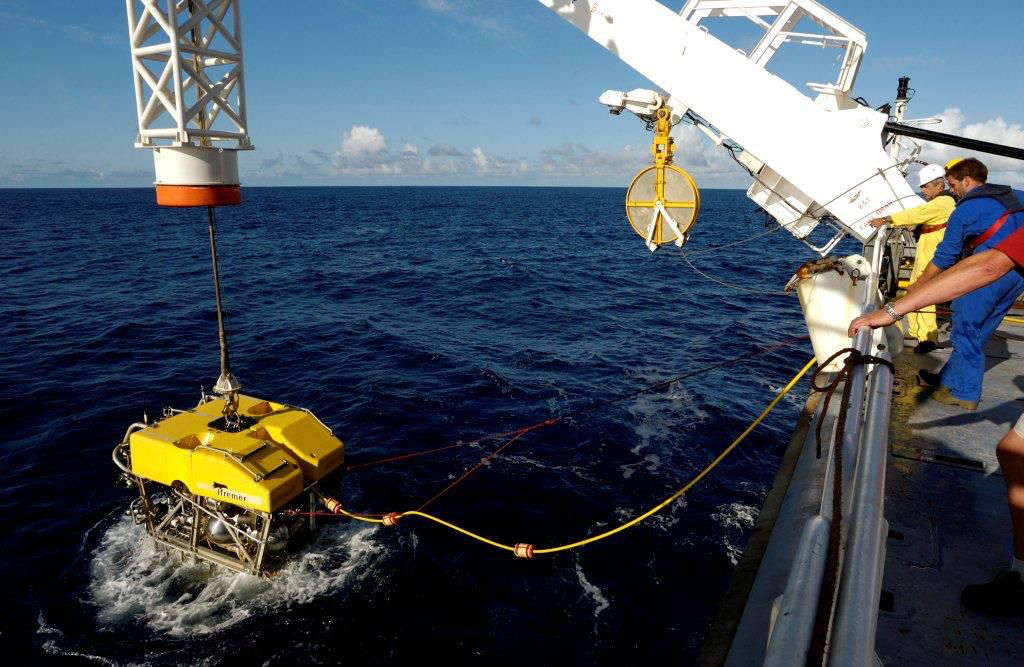
\includegraphics[width=.45\linewidth]{Victor6000-ROV}} \quad
	\subfloat[]{
		\label{fig:Victor6000-ROV-Ship}
		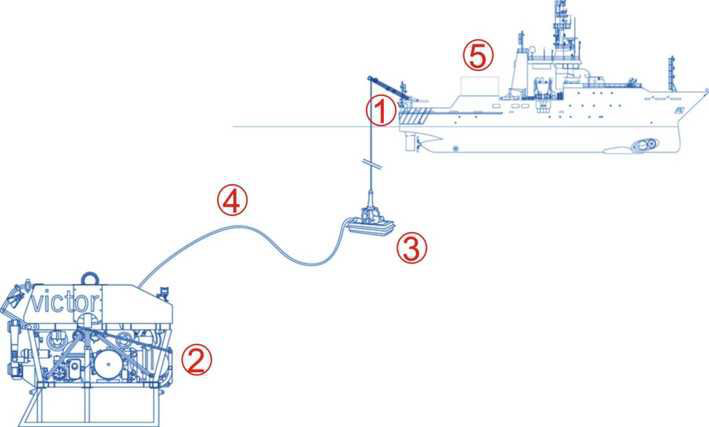
\includegraphics[width=.45\linewidth]{Victor6000-ROV-Ship}}
\caption[VICTOR 6000: a remotely operated vehicle (ROV) and its surface vessel.]
{\subref{fig:victor6000-rov} The VICTOR 6000 ROV.
\subref{fig:Victor6000-ROV-Ship} The ROV-vessel system: 1) a direct-winding
winch, 2) the ROV, 3) the hard ballast, 4) the tether
cable, and 5) the power/hydraulic units and control room. Image
credit: Ifremer.
%\url{http://flotte.ifremer.fr/fleet/Presentation-of-the-fleet/Underwater-systems/VICTOR-6000}
}
\label{fig:rov}
\end{figure}

The second group gathers the \acp{AUV}, or \acp{UUV} that do not require being
controlled by a human operator. This characteristic eliminates the need of
continuously being in contact with a surface mother ship, thus permitting to
overcome some major drawbacks of the former group, such as their high operative
cost and limited working area. In most of the \ac{AUV} applications, the vehicle
follows a sequence of pre-calculated waypoints and uses its onboard sensors to
gather oceanographic information of biological nature~\cite{Grasmueck2006},
chemical composition~\cite{WeiLi2006}, and even archaeological
data~\cite{Bingham2010}. Often, they are also equipped with multibeam and
imaging sonars that collect data that is used to build bathymetric maps
(\ie elevation maps of the seabed). These underwater surveys are normally
conducted in a previously explored area so that the vehicle navigates at a
constant and safe altitude from the seafloor.

Furthermore, \acp{AUV} can also be divided into two main subcategories:
buoyancy-driven and propeller-driven. The former category corresponds to the
underwater gliders, or \acp{AUV} that are capable of modifying its buoyancy in
order to generate sinusoidal-like vertical motion that, together with their
wings, also permit horizontal (forward and lateral) motion. The trajectories
followed by these vehicles also include periodic ascents to the surface to
obtain GPS fixes, thus improving its navigation estimation (see
Fig.~\ref{fig:GliderAUV}). This propulsion technique results in a
low-consumption but also less maneuverable approach. This is commonly used in
long-term studies over open sea areas, in which a single mission can last from
days to weeks.

\begin{figure}[htbp]
	\centering
	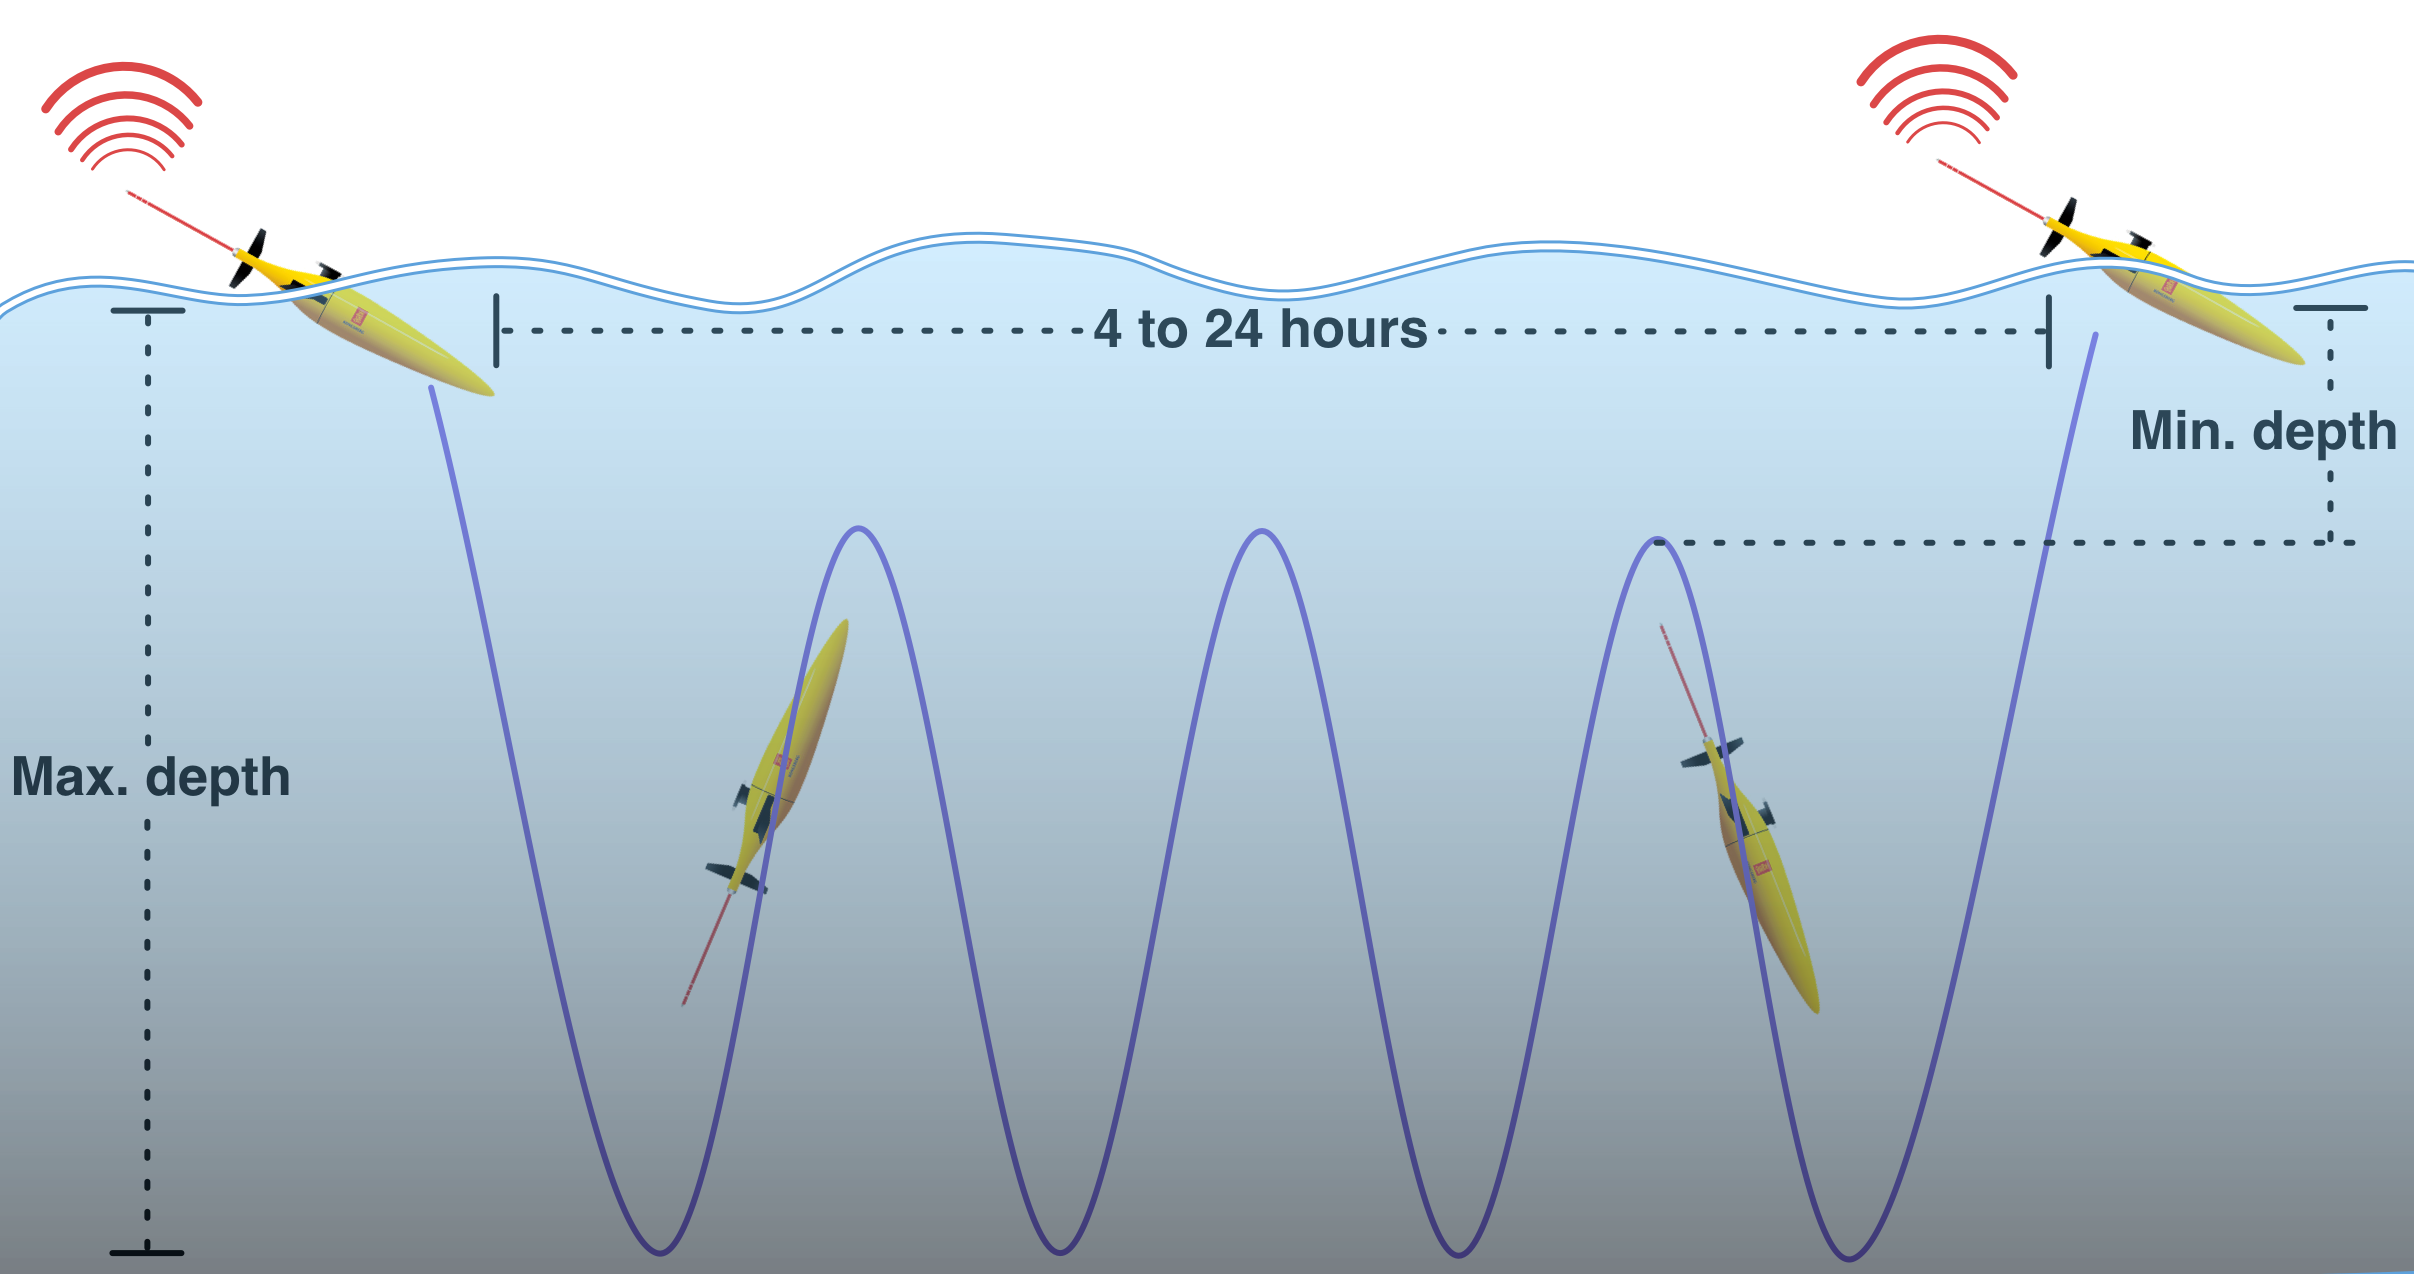
\includegraphics[width=.8\linewidth]{SeagliderAUV} \quad
\caption[Underwater glider and its sinusoidal-like vertical motion.]
{Underwater glider, or AUV with the capability of modifying its buoyancy to
generate sinusoidal-like vertical motion. The vehicle dives for several hours to
gather data, and surfaces periodically to obtain GPS fixes thus improving its
own navigation estimation.}
\label{fig:GliderAUV}
\end{figure}

The propeller-driven \acp{AUV}, on the other hand, correspond to those that use
propellers or thrusters to generate \ac{3D} motions. The work presented
throughout this thesis is dedicated to this latter kind of vehicles.
Furthermore, it has been mainly validated with the Sparus~II, a torpedo-shaped
\ac{AUV} (see Fig.~\ref{fig:Sparus2}).

\begin{figure}[htbp]
	\centering
	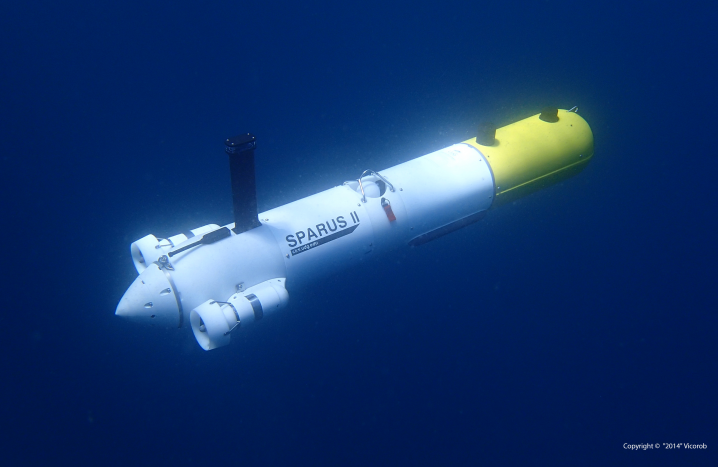
\includegraphics[width=.6\linewidth]{Sparus2} \quad
\caption[Sparus~II: a torpedo-shaped and propeller-driven autonomous underwater
vehicle (AUV).]
{Sparus~II AUV, a torpedo-shaped and propeller-driven underwater vehicle, which
is equipped with two back thrusters for horizontal motion, and one independent
thruster for vertical motion.}
\label{fig:Sparus2}
\end{figure}

% \begin{figure}[bth]
%         \myfloatalign
%         \subfloat[Asia personas duo.]
%         {\includegraphics[width=.45\linewidth]{gfx/example_1}} \quad
%         \subfloat[Pan ma signo.]
%         {\label{fig:example-b}%
%          \includegraphics[width=.45\linewidth]{gfx/example_2}} \\
%         \subfloat[Methodicamente o uno.]
%         {\includegraphics[width=.45\linewidth]{gfx/example_3}} \quad
%         \subfloat[Titulo debitas.]
%         {\includegraphics[width=.45\linewidth]{gfx/example_4}}
%         \caption[Tu duo titulo debitas latente]{Tu duo titulo debitas
%         latente. \ac{DRY}}\label{fig:example}
% \end{figure}

\section{Problem Statement}

Recent \ac{AUV} applications include imaging and inspecting different kinds of
structures such as in-water ship hulls~\cite{Hover2012,Hurtos2015} and natural
structures on the sea floor~\cite{Galceran2014b}. These applications share a
common characteristic: they require \textit{a priori} information of the area or
structure to be inspected. Therefore it is needed to either navigate at a safe
and conservative altitude~\cite{Grasmueck2006,Bingham2010} or to pre-calculate a
survey path that may be corrected or reshaped
online~\cite{Hover2012,Galceran2014b}. However, there are similar or even
potentially new applications, such as exploring confined natural environments
(\eg underwater caves)~\cite{Mallios2015}, where such information might not be
available. In these scenarios, the \ac{AUV} must operate in unexplored
(unknown), cluttered and dynamic environments, and therefore are more exposed to
collisions.

Although the aforementioned \ac{AUV} applications share some common requirements
with aerial and terrestrial robots (\eg localization, mapping, vision, etc.),
navigating autonomously while conducting such type of tasks in an underwater
environment presents different challenges. These are caused by factors specific
to this environment, such as the presence of external disturbances (currents),
low-range visibility and limited navigation accuracy. Dealing with such
constraints requires a path planner with online computation capabilities, which
contribute in overcoming the lack of surroundings information and the global
position inaccuracy, especially when navigating in close proximity to nearby
obstacles.

\subsection{Navigating in Unexplored Environments with AUVs}

Even with the most recent technological advances, conducting both teleoperated
and autonomous missions in underwater environments still represents a challenge
with different scientific aspects to be solved. One important restriction faced
by \acp{UUV} is that they operate in GPS-denied environments, which limits their
capability to accurately calculate their position with respect to an inertial
reference frame. In order to cope with this, \ac{DR} techniques are used to
estimate the relative position with respect to an initial position, which is
normally defined from GPS fixes obtained when the vehicle is at surface. This
approach suffices in many survey \ac{AUV} applications. However, its limitations
rely on highly precise odometry and low-level or negligible disturbances. When
these conditions are not met, it can rapidly lead to errors in distance
estimation, which make this approach an unsafe alternative when navigating and
exploring surroundings in close proximity to nearby obstacles, even when the
environment is known and a map is available.

Another alternative is the of use of an \ac{USBL}, which is a method of
underwater acoustic positioning. An \ac{USBL} system is composed of a
transceiver mounted on a surface vessel and a transponder mounted on the
\ac{AUV}. This system permits calculating the range (distance) and the angle of
the subsea vehicle with respect to the surface vehicle. Furthermore, given that
the transceiver is at surface (\ie it can get GPS fixes), it is possible to
calculate a more accurate absolute position of the \ac{AUV}. The major drawback
of this alternative is the mobility constraint imposed by the transceiver,
similar to what occurs with a \ac{ROV} and its mother ship. This also prevents
its use in confined natural environments such as an underwater caves complex,
which results in a critical limitation for the new applications intended for
\acp{AUV}.

Therefore, when planning collision-free \ac{AUV} paths, the difficulty to
pre-explore and build a map of the area or structure of interest is an
additional challenge to be considered together with the navigation inaccuracy.
In order to tackle these problems, this thesis proposes a framework that endows
an \ac{AUV} with the capability to map an undiscovered environment, while
planning collision-free paths to navigate throughout it. Furthermore, although
the framework considers specific characteristics of the motion planning problem
for \acp{AUV}, the proposed approach may also be applied for other types of
autonomous vehicles.

\subsection{Path/Motion Planning Problem for AUVs}

\subsubsection{Overview of the Basic Robot Path/Motion Planning}

In general, path/motion planning methods can be divided into two categories
according to their application: coverage planning and start-to-goal planning.
The former category, commonly referred to as \ac{CPP}, gathers those methods
that seek to determine a collision-free path that a robot must follow in order to
pass over all points of an area or volume of interest. A detailed review of
available techniques that address this problem can be found
in~\cite{Galceran2013a}.

The second category, \ie start-to-goal motion planning, consists in finding
valid (collision-free) paths from a start configuration to a goal configuration
in the \ac{C-Space}, which is the space of all the possible robot
configurations~\cite{Lozano-Perez1983}. There are different computational
algorithms that attempt to solve this task. Some of them find an analytic
solution, but their applicability is limited to simple problems. Another group
of algorithms, such as Dijkstra's~\cite{Dijkstra1959}, A*~\cite{Hart1968} and
D*~\cite{Stentz1994}, search throughout discretization of the \ac{C-Space}.
However, in problems involving high-dimensional \acp{C-Space}, these exhaustive
search methods suffer from scalability issues.

One alternative in dealing with this is to use the so-called sampling-based
methods. These latter ones construct a partial representation by taking samples
at random from the \ac{C-Space} and checking them for
collisions~\cite{Choset2005,LaValle2006}, instead of fully describing the
\ac{C-Space}. In contrast with exhaustive search methods, these are not complete
(\ie they can not report whether a solution exists), but often find a
solution for complex problems where other algorithms fail.

There are additional characteristics or capabilities that should be considered
when solving path/motion planning tasks for \acp{AUV}. Some of which will be
mentioned in the following sections.

\subsubsection{Planning under Geometric and Differential (Motion) Constraints}
\label{sec:PlannUnderConst}

When calculating a valid path, the planner must deal with different types of
constraints, some of which may be related only to the \ac{C-Space}, while others
may also include the vehicle motion capabilities. Depending on which constraints
are considered, the planning problem was categorized in one of two possible
groups: geometric path planning and motion planning ~\cite{Choset2005}. The
former group assumes that the robotic system can move instantaneously in any
direction (\ie system kinematics and dynamics are negligible), thus reducing the
problem to geometric constraints that are solved by checking for collisions over
the \ac{C-Space}.

However, the motion constraints associated with the vehicle are often
significant, and therefore the robot is not capable of following a simple
geometric path. This means that, when calculating collision-free paths, it is
necessary to use a vehicle motion model that includes differential constraints,
also called kinodynamic constraints. Such a group of planning problems is
commonly called motion planning or \textit{kinodynamic motion planning} (this
latter term was introduced by Donald \etal in 1993~\cite{Donald1993}). An
example of such planning problems is the one related to a non-holonomic
torpedo-shaped \ac{AUV}, as the ones used in this thesis (see
Figure~\ref{fig:Sparus2}).

As recently the terms path planning and motion planning are used
interchangeably~\cite{Sucan2011},~\cite{LaValle2006}, throughout this thesis, we
refer to the either problem as path/motion planning

\subsubsection{3D Path/Motion Planning}

In some \ac{AUV} applications the vehicle either navigates at constant depth or
attempts to keep reference values of altitude. In those cases, and specially in
areas with no or little relief, it is possible to simplify the motion model to
one that assumes the vertical position variation as constant or negligible.
Nonetheless, when such conditions are not met, it is required to use more
complete motion equations, which in the simplest case implies adding an
additional state variable for the vertical motion, or in more complex scenarios
may require to use a \ac{6D} state space, \ie one that incorporates the position
and the orientation of the vehicle in a \ac{3D} workspace, where each state or
configuration is $q = [x,y,z, \phi, \theta, \psi]$.
 
\subsubsection{Online Path/Motion Planning}

Another important aspect to be considered when planning motions for \acp{AUV},
especially when navigating in unexplored environments, is the necessity of
calculating the paths (motions) online. To deal with such computation
constraints, the planner must be capable of providing a solution at \textit{any
time} and of correcting (reshaping) it according to the updated environment
information gathered along the mission execution. This characteristic implies
that although it is possible that the solution provided at \textit{any time} may
not be the most optimal one, any available time left will be spent on improving
the existing solution path. This means that the next delivered solution is
better than the previous one or at least equally good. Finally, it is also
important to correctly balance the computation load to coexist with other
functional modules of the \ac{AUV} such as navigation, control, etc.

\section{Objectives of the Thesis}

Once the motivation and the most relevant aspects of the problem addressed in
this thesis have been established, the main objective of this work can be stated
as follows:

\bigskip

\noindent \textit{To endow an \acf{AUV} with the capability to incrementally map
an unexplored environment, while planning online collision-free paths; such paths
should be \acf{3D}, safe, and feasible (doable) according to the vehicle's
motion constraints. This will contribute a further step towards better and more
reliable \acp{AUV} for the new and potential applications.}

\bigskip

This objective can be separated into the following specific
objectives:

\bigskip

\noindent\textbf{Review of the Path/Motion Planning Literature:} To conduct a
review of the most relevant path/motion planning methods, which have been used
for different robotic systems including terrestrial, aerial, and, especially,
marine vehicles. This will allow identifying the most appropriate approaches for
meeting the aforementioned constraints for the intended applications.

\bigskip

\noindent\textbf{Planning Feasible Motions for AUVs:} To propose a motion
planning method that takes into account the \ac{AUV}'s motion constraints for
both 2D and 3D movements. This will permit generating more feasible motions
according to the \ac{AUV}'s capabilities. Furthermore, such motions will be more
likely to be followed by the vehicle, thus minimizing unexpected maneuvers.

\bigskip

\noindent\textbf{Online Mapping and Path/Motion Planning for AUVs:} To propose a
framework that allows an \ac{AUV} to safely navigate through initially
unexplored environments. This implies that the vehicle must be capable of
incrementally mapping the surroundings while, simultaneously and online,
planning safe and feasible paths.

\bigskip

\noindent\textbf{Simulation and In-water Validation:} To extensively test and
validate the proposed approach in different simulated and real-world scenarios.

\section{Thesis Outline and Contributions}

This manuscript is organized in a way that presents the incremental and
progressive development of this thesis. In order to contextualize and better
understand the real impact of such developments,
Chapter~\ref{ch:state_of_the_art} firstly makes a review of the most relevant
methods, techniques, and applications that compose the state of the art, not
only in what has to do with path/motion planning, but also in relation with the
approaches currently applied with \acp{AUV}. Then, based on the new and
potential applications intended for \acp{AUV} that were mentioned above, and
considering their requirements, the main contributions of this thesis are
gathered and distributed throughout this document as follows:

\begin{inparaenum}[1)]

\item The incorporation of motion constraints into the \ac{AUV} path planner,
which acts as a mechanism to avoid generating unfeasible paths, thus reducing
the number of unexpected maneuvers. This includes those constraints required for
constant depth missions that only take into account \ac{2D} horizontal motions,
which are discussed in Chapter~\ref{ch:motion_constratins}. But it includes as
well more challenging and variable depth missions that require analysing and
combining the vehicle turning and ascending/descending limitations, which are
addressed in Chapter~\ref{ch:planning_3D}.

\item An efficient approach for approximating the risk associated with a path.
There are situations in which considering the vehicle motion constraints does
not avoid risky maneuvers, especially when navigating in close proximity to
nearby obstacles. In such cases, the \ac{AUV} path/motion planner must lead the
vehicle to navigate at a safe and conservative distance from its surroundings,
yet without discarding any possible solution. Different strategies to estimate
the risk associated with a vehicle configuration, and therefore with a path, are
presented and compared in Chapter~\ref{ch:plann_online}.

\item The capability of an \ac{AUV} to efficiently (re)plan feasible and safe
paths, \ie under motion constraints and taking into consideration the associated
risk, in scenarios where the environment is incrementally discovered.
This clearly means that the path/motion planner has to operate under online
computation constraints, which can only be done by combining existing approaches
and newly proposed strategies, such as \textit{opportunistic state checking}
and \textit{reuse of the last best known solution}. The complete online
planning approach will be presented in Chapter~\ref{ch:plann_online}.

\item A framework that allows an \ac{AUV} to incrementally map an environment
undiscovered previously, while simultaneously (re)planning a path that must be
followed by the vehicle to safely cross and explore the surroundings. This
framework integrates all previous stages and characteristics, in order to
finally endow the \ac{AUV} with the required capabilities for the intended
applications, and will also be presented in Chapter~\ref{ch:plann_online}.

\item An extensive validation of the proposed framework is presented in
Chapter~\ref{ch:applications}. This includes simulated and in-water trials in
different real-world scenarios, where an \ac{AUV} had to navigate through
initially unexplored environments, while gathering different kind of information
such as acoustic and optical data. These tests were conducted with two different
\acp{AUV}: the Sparus~II from the University of Girona, and the AsterX from the
\ac{Ifremer}\footnote{Technical details about both vehicles can be found in
Appendix~\ref{appx:exp_platform}.}. The results include planning safe and
feasible paths to move through both artificial and natural marine structures, as
well as the autonomous survey replanning for gap filling and target inspection.

\end{inparaenum}

Finally, concluding remarks and directions for further research are given and
discussed in Chapter~\ref{ch:conclusions}.

% intro
% Write your text without any further commands, like this:.... Any organised
% system requires energy, be it a machine of some kind or a live organism. Energy
% is needed to win the uphill battle against entropy and pull together lifeless
% molecules to be able to do something in this world, like complete a PhD.


%: ----------------------- HELP: lists
% This is how you generate lists in LaTeX.
% If you replace {itemize} by {enumerate} you get a numbered list.

% \subsection{Name your subsection} % subsection headings are again smaller than section names
% lead
% Different organised systems have different energy currencies. The machines that
% enable us to do science like sizzling electricity but at a controlled voltage.
% Earth's living beings are no different, except that they have developed another
% preference. They thrive on various chemicals.
% 
% % dextran, starch, glycogen
% Most organisms use polymers of glucose units for energy storage and differ only
% slightly in the way they link together monomers to sometimes gigantic
% macromolecules. Dextran of bacteria is made from long chains of
% $\alpha$-1,6-linked glucose units.

%: ----------------------- HELP: special characters
% above you can see how special characters are coded; e.g. $\alpha$
% below are the most frequently used codes:
%$\alpha$  $\beta$  $\gamma$  $\delta$

%$^{chars to be superscripted}$  OR $^x$ (for a single character)
%$_{chars to be suberscripted}$  OR $_x$

%>  $>$  greater,  <  $<$  less
%≥  $\ge$  greater than or equal, ≤  $\ge$  lesser than or equal
%~  $\sim$  similar to

%$^{\circ}$C   ° as in degree C
%±  \pm     plus/minus sign

%$\AA$     produces  Å (Angstrom)




% % dextran, starch, glycogen continued
% Starch of plants and glycogen of animals consists of $\alpha$-1,4-glycosidic
% glucose polymers \cite{lastname07}. See figure \ref{largepotato} for a
% comparison of glucose polymer structure and chemistry.
% 
% Two references can be placed separated by a comma \cite{lastname07,name06}.

%: ----------------------- HELP: references
% References can be links to figures, tables, sections, or references.
% For figures, tables, and text you define the target of the link with \label{XYZ}. Then you call cross-link with the command \ref{XYZ}, as above
% Citations are bound in a very similar way with \cite{XYZ}. You store your references in a BibTex file with a programme like BibDesk.





% \figuremacro{MorphProject}
% {A common glucose polymers}
% {The figure shows starch granules in potato cells, taken from
% \href{http://molecularexpressions.com/micro/gallery/burgersnfries/burgersnfries4.html}{Molecular
% Expressions}.}

%: ----------------------- HELP: adding figures with macros
% This template provides a very convenient way to add figures with minimal code.
% \figuremacro{1}{2}{3}{4} calls up a series of commands formating your image.
% 1 = name of the file without extension; PNG, JPEG is ok; GIF doesn't work
% 2 = title of the figure AND the name of the label for cross-linking
% 3 = caption text for the figure

%: ----------------------- HELP: www links
% You can also see above how, www links are placed
% \href{http://www.something.net}{link text}

% \figuremacroW{largepotato}{Title}{Caption}{0.8}
% variation of the above macro with a width setting
% \figuremacroW{1}{2}{3}{4}
% 1-3 as above
% 4 = size relative to text width which is 1; use this to reduce figures




% Insulin stimulates the following processes:
% 
% \begin{itemize}
% \item muscle and fat cells remove glucose from the blood,
% \item cells breakdown glucose via glycolysis and the citrate cycle, storing its energy in the form of ATP,
% \item liver and muscle store glucose as glycogen as a short-term energy reserve,
% \item adipose tissue stores glucose as fat for long-term energy reserve, and
% \item cells use glucose for protein synthesis.
% \end{itemize}

%: ----------------------- HELP: lists
% This is how you generate lists in LaTeX.
% If you replace {itemize} by {enumerate} you get a numbered list.


 


%: ----------------------- HELP: tables
% Directly coding tables in latex is tiresome. See below.
% I would recommend using a converter macro that allows you to make the table in Excel and convert them into latex code which you can then paste into your doc.
% This is the link: http://www.softpedia.com/get/Office-tools/Other-Office-Tools/Excel2Latex.shtml
% It's a Excel template file containing a macro for the conversion.

% \begin{table}[htdp]
% \centering
% \begin{tabular}{ccc} % ccc means 3 columns, all centered; alternatives are l, r
% 
% {\bf Gene} & {\bf GeneID} & {\bf Length} \\ 
% % & denotes the end of a cell/column, \\ changes to next table row
% \hline % draws a line under the column headers
% 
% human latexin & 1234 & 14.9 kbps \\
% mouse latexin & 2345 & 10.1 kbps \\
% rat latexin   & 3456 & 9.6 kbps \\
% % Watch out. Every line must have 3 columns = 2x &. 
% % Otherwise you will get an error.
% 
% \end{tabular}
% \caption[title of table]{\textbf{title of table} - Overview of latexin genes.}
% % You only need to write the title twice if you don't want it to appear in bold in the list of tables.
% \label{latexin_genes} % label for cross-links with \ref{latexin_genes}
% \end{table}



% There you go. You already know the most important things.


% ----------------------------------------------------------------------




%\cleardoublepage
%% this file is called up by thesis.tex
% content in this file will be fed into the main document

\chapter{State of the Art} % top level followed by section, subsection
\label{ch:state_of_the_art}
%************************************************

% the code below specifies where the figures are stored
\ifpdf
    \graphicspath{{2_state_of_the_art/figures/PNG/}{2_state_of_the_art/figures/PDF/}{2_state_of_the_art/figures/}}
\else
    \graphicspath{{2_state_of_the_art/figures/EPS/}{2_state_of_the_art/figures/}}
\fi

% ----------------------- contents from here ------------------------

Although the major research efforts in this thesis were focused on developing,
extending and using path/motion planning methods for \ac{AUV} applications,
their validation with an \ac{AUV} in real-world scenarios involved other fields
of study. These included but were not limited to: navigation, perception,
mapping and control. An extensive presentation of the state-of-the-art
background of all these areas would not only prove to be lengthy and diffuse,
but would also be out of the scope of this work. Nonetheless, this chapter is
dedicated to contextualizing the contribution of this thesis. In order to do so,
it firstly provides a survey of the techniques available for solving
specifically path/motion planning problems. Secondly, it discusses the most
common extensions used when the vehicle motion capabilities have to be taken
into consideration or when dealing with online computation constraints.
Finally, it presents a review of the algorithms and extensions that have been
used with \acp{AUV} particularly.

\section{Planning Collision-free Paths over the C-Space}

Even though first works on path/motion planning appeared in the late
60's~\cite{Nilsson1969}, it was only until the 80's, when Lozano-Perez
introduced the concept of the \textit{configuration
space}~\cite{Lozano-Perez1983,Lozano-Perez1984,Lozano-Perez1987}, that this
field of study became active. The configuration space (or \ac{C-Space})
establishes the set of all possible \textit{configurations} that a robot can
adopt when executing tasks in the workspace. While the workspace, $\mathcal{W}$,
is typically defined as $\mathbb{R}^n$ (where $n=2,3$ for \ac{2D} and \ac{3D}
motion, respectively), the \ac{C-Space}, $\mathcal{C}$, depends on the robot
motion capabilities. For example, a robot considered to be a point that moves in
a plane (\ie $\mathcal{W}=\mathbb{R}^2$) requires two coordinates in order to
specify its \textit{configuration}, $q$,  which is equal to $[x,y]^T$, thus $q
\in \mathcal{C}=\mathbb{R}^2$. 

However, if the robot is considered to be a rigid body that moves in a plane
(\ie in the same $\mathcal{W}$), it requires three coordinates; these would
describe not only its position, but also its orientation, therefore its
\textit{configuration} is now $q=[x,y,\psi]^T$, which is commonly expressed as
$q \in \mathcal{C} = SE(2) = \mathbb{R}^2 \times SO(2) = \mathbb{R}^2 \times
\mathcal{S}$. A similar scenario occurs with a single rigid-body robot that
operates in \ac{3D} workspaces, in which $q = [x,y,z]$, so that $q \in
\mathcal{C}=\mathbb{R}^3$ when only the robot´s position is considered, or $q =
[x,y,z, \phi, \theta, \psi]$, so that $q \in \mathcal{C} = SE(3) = \mathbb{R}^3
\times SO(3)$ when considering both position and orientation. Finally, when the
robot is an articulated rigid body system, for instance a manipulator arm, a
given \textit{configuration} is described by the values of a set of $n$
generalized coordinates $q = q_1, \ldots , q_n$, corresponding to each of the
robotic arm \acp{DOF}.

The solution to a simple path/motion planning problem, which requires connecting
a start and a goal configuration, $q_{start}$ and $q_{goal}$, is a continuous
path $p:[0,1] \rightarrow \mathcal{C}$, such that $p(0)=q_{start}$ and
$p(1)=q_{goal}$. However, a robot generally conducts tasks in environments that
contain obstacles, which normally are to be avoided. For this reason, the
\ac{C-Space} is subdivided into \textit{free space} ($\mathcal{C}_{free}$) and
the \textit{obstacle region} ($\mathcal{C}_{obs}$), meaning that $\mathcal{C} =
\mathcal{C}_{free} \cup \mathcal{C}_{obs}$. Therefore, a collision-free path is
defined as a continuous path $p:[0,1] \rightarrow \mathcal{C}_{free}$. This
concept is illustrated in Figure~\ref{fig:collision-free-path}.

\begin{figure}[htbp]
	\centering
	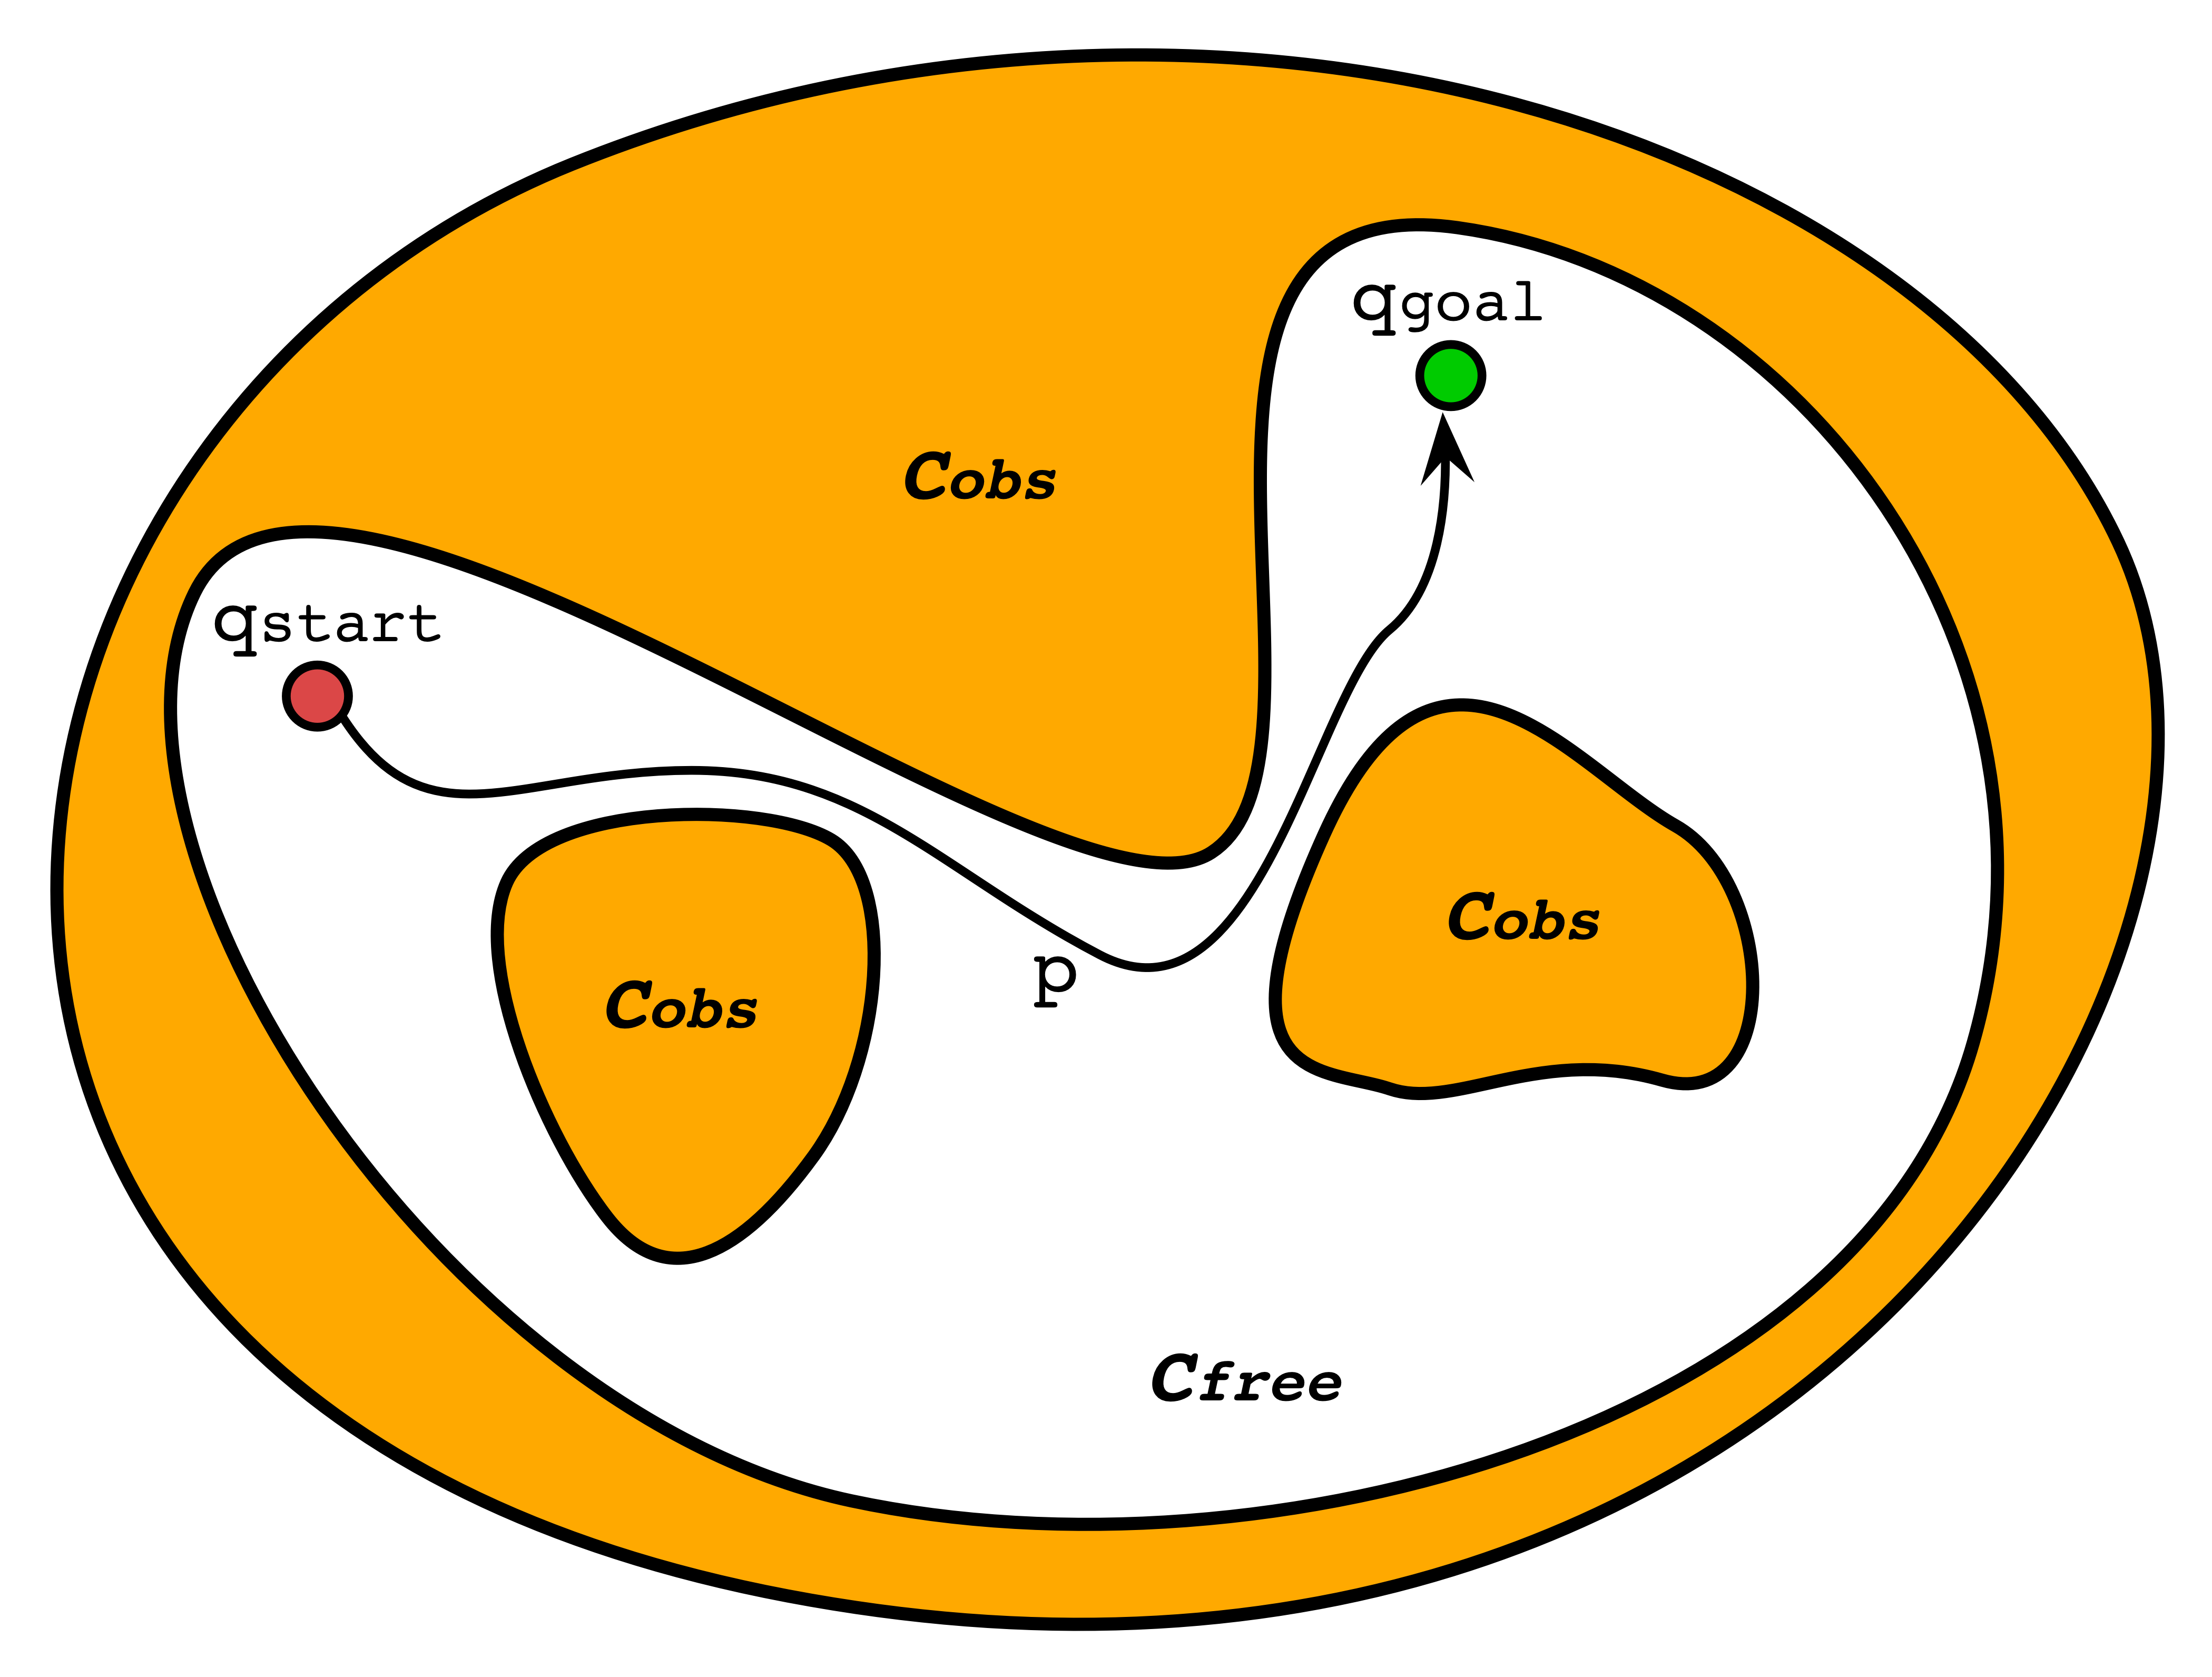
\includegraphics[width=.75\linewidth]{collision-free-path}
\caption[The basic path/motion planning problem and the C-Space concept.]
{The basic path/motion planning problem seeks to connect a start configuration
($q_{start}$) and goal configuration ($q_{goal}$) with a continuous
collision-free path $p:[0,1] \rightarrow \mathcal{C}_{free}$.}
\label{fig:collision-free-path}
\end{figure}

% ----------------------- another section  ------------------------
\section{Bug-based Methods}

Bug-based methods represent one of the earliest reactive and sensor-based path
planning approaches, in which a mobile robot moves in the plane towards a global
goal, while having a limited (local) knowledge of the environment. The
algorithms included in this group are based on two basic behaviors: go straight
towards the goal and follow the obstacles' boundary. Lumelsky and Stepanov
presented the first of these algorithms, known as Bug1 and Bug2, that mainly
rely on tactile or zero range sensors to perceive the
obstacles~\cite{Lumelsky1987}. Later, Kamon \etal introduced the Tangent Bug
algorithm, which is an extension that uses non-zero range
sensors~\cite{Kamon1996}. All of them are classified as complete algorithms,
which means that they find a solution when one is possible or, otherwise, they
report when there is no solution. Furthermore, they assume the robot is a point
that moves in a \ac{2D} workspace, and that it is capable of knowing its
position and calculating its distance to the goal.

Bug1~\cite{Lumelsky1987} is the most basic algorithm that uses the
aforementioned behaviors. With this method, the robot moves from the start
position ($q_{start}$) towards the desired goal position ($q_{goal}$) until it
reaches the goal or until it finds an obstacle (detected with its tactile
sensors). When the latter situation occurs, the robot stores its current
position and marks it as the \textit{hit point} ($H_i$). Then it changes its
motion mode (behavior) to completely circumnavigate the obstacle. While the
vehicle follows the obstacle boundary, it continuously calculates the distance
to the goal in order to determine the position that corresponds to the minimum
possible distance. This is marked as the \textit{leave point} ($L_i$). Once the
robot reaches the \textit{hit point} again (\ie after it has traveled all the
obstacle contour), it goes back to the \textit{leave point} and there changes
its behavior, once again, in order to move towards the goal. This procedure is
repeated until reaching the specified goal. Figure~\ref{fig:Bug1} depicts an
example of this algorithm solving a start-to-goal query.

\begin{figure}[htbp]
	\centering
	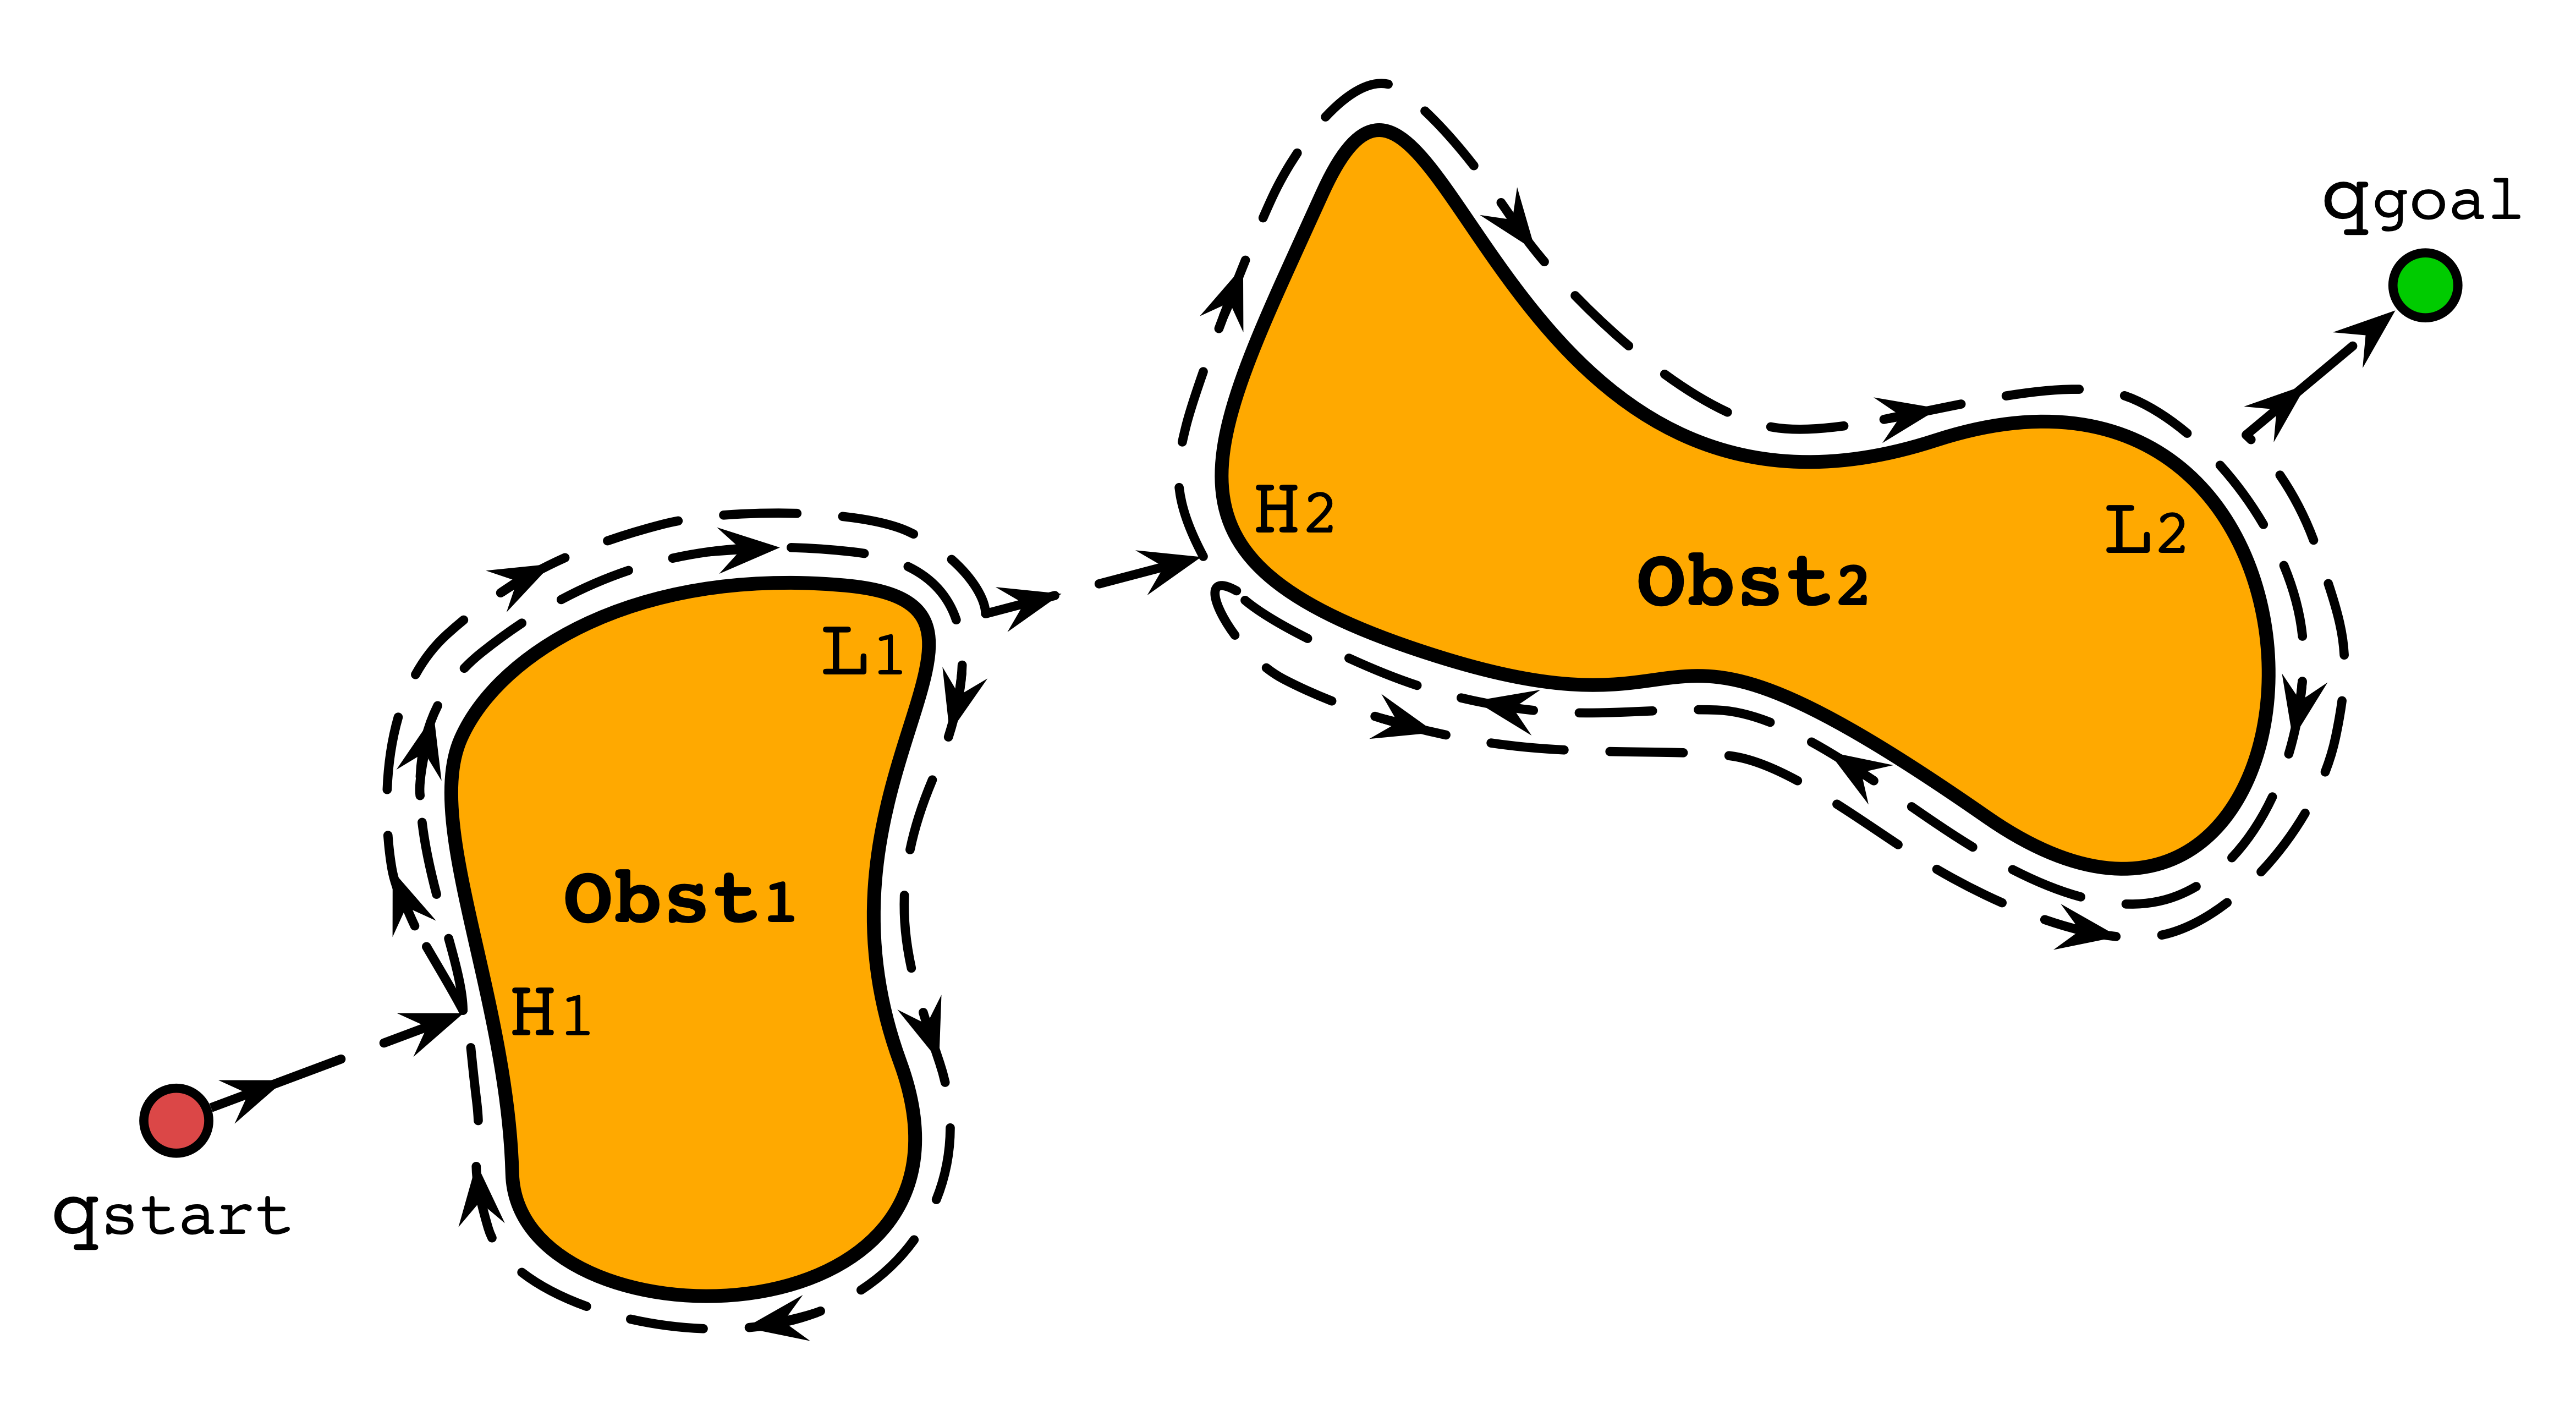
\includegraphics[width=.75\linewidth]{Bug1} \quad
\caption[Reactive and sensor-based method Bug1.]
{Reactive and sensor-based method Bug1}
\label{fig:Bug1}
\end{figure}

Bug2~\cite{Lumelsky1987} attempts to be an improved version of the previously
explained algorithm. It establishes a straight line, sometimes referred as the
\textit{m-line}~\cite{Choset2005}, which connects the start and goal positions.
With this algorithm, the robot starts moving towards the desired goal by
following the \textit{m-line} until it reaches the goal or finds an obstacle. As
occurs with Bug1, if the robot is dealing with an obstacle, it first marks that
position as the \textit{hit point} ($H_i$) and then changes its behavior to
circumnavigate the obstacle. However, with Bug2 the robot does not necessarily
travel the entire obstacle boundary, but instead stops when reaching another
point in the \textit{m-line}; if such a point is closer to the goal than the
previous \textit{hit point}, the robot marks this position as \textit{leave
point} ($L_i$) and, from there, continues following the \textit{m-line} towards
the goal. This procedure is repeated until reaching the specified goal. Even
though Bug2 does not require to completely circumnavigate the obstacles, there
are environments where the robots do require to travel the entire boundary; in
these cases Bug2 may generate longer paths than those calculated by Bug1, and
therefore is less efficient. Figure~\ref{fig:Bug2} depicts an example of Bug2
solving start-to-goal queries in both simple and complex scenarios.

\begin{figure}[htbp]
    \myfloatalign
    \subfloat[Bug2 simple scenario]
    {\label{fig:Bug2-simple}
    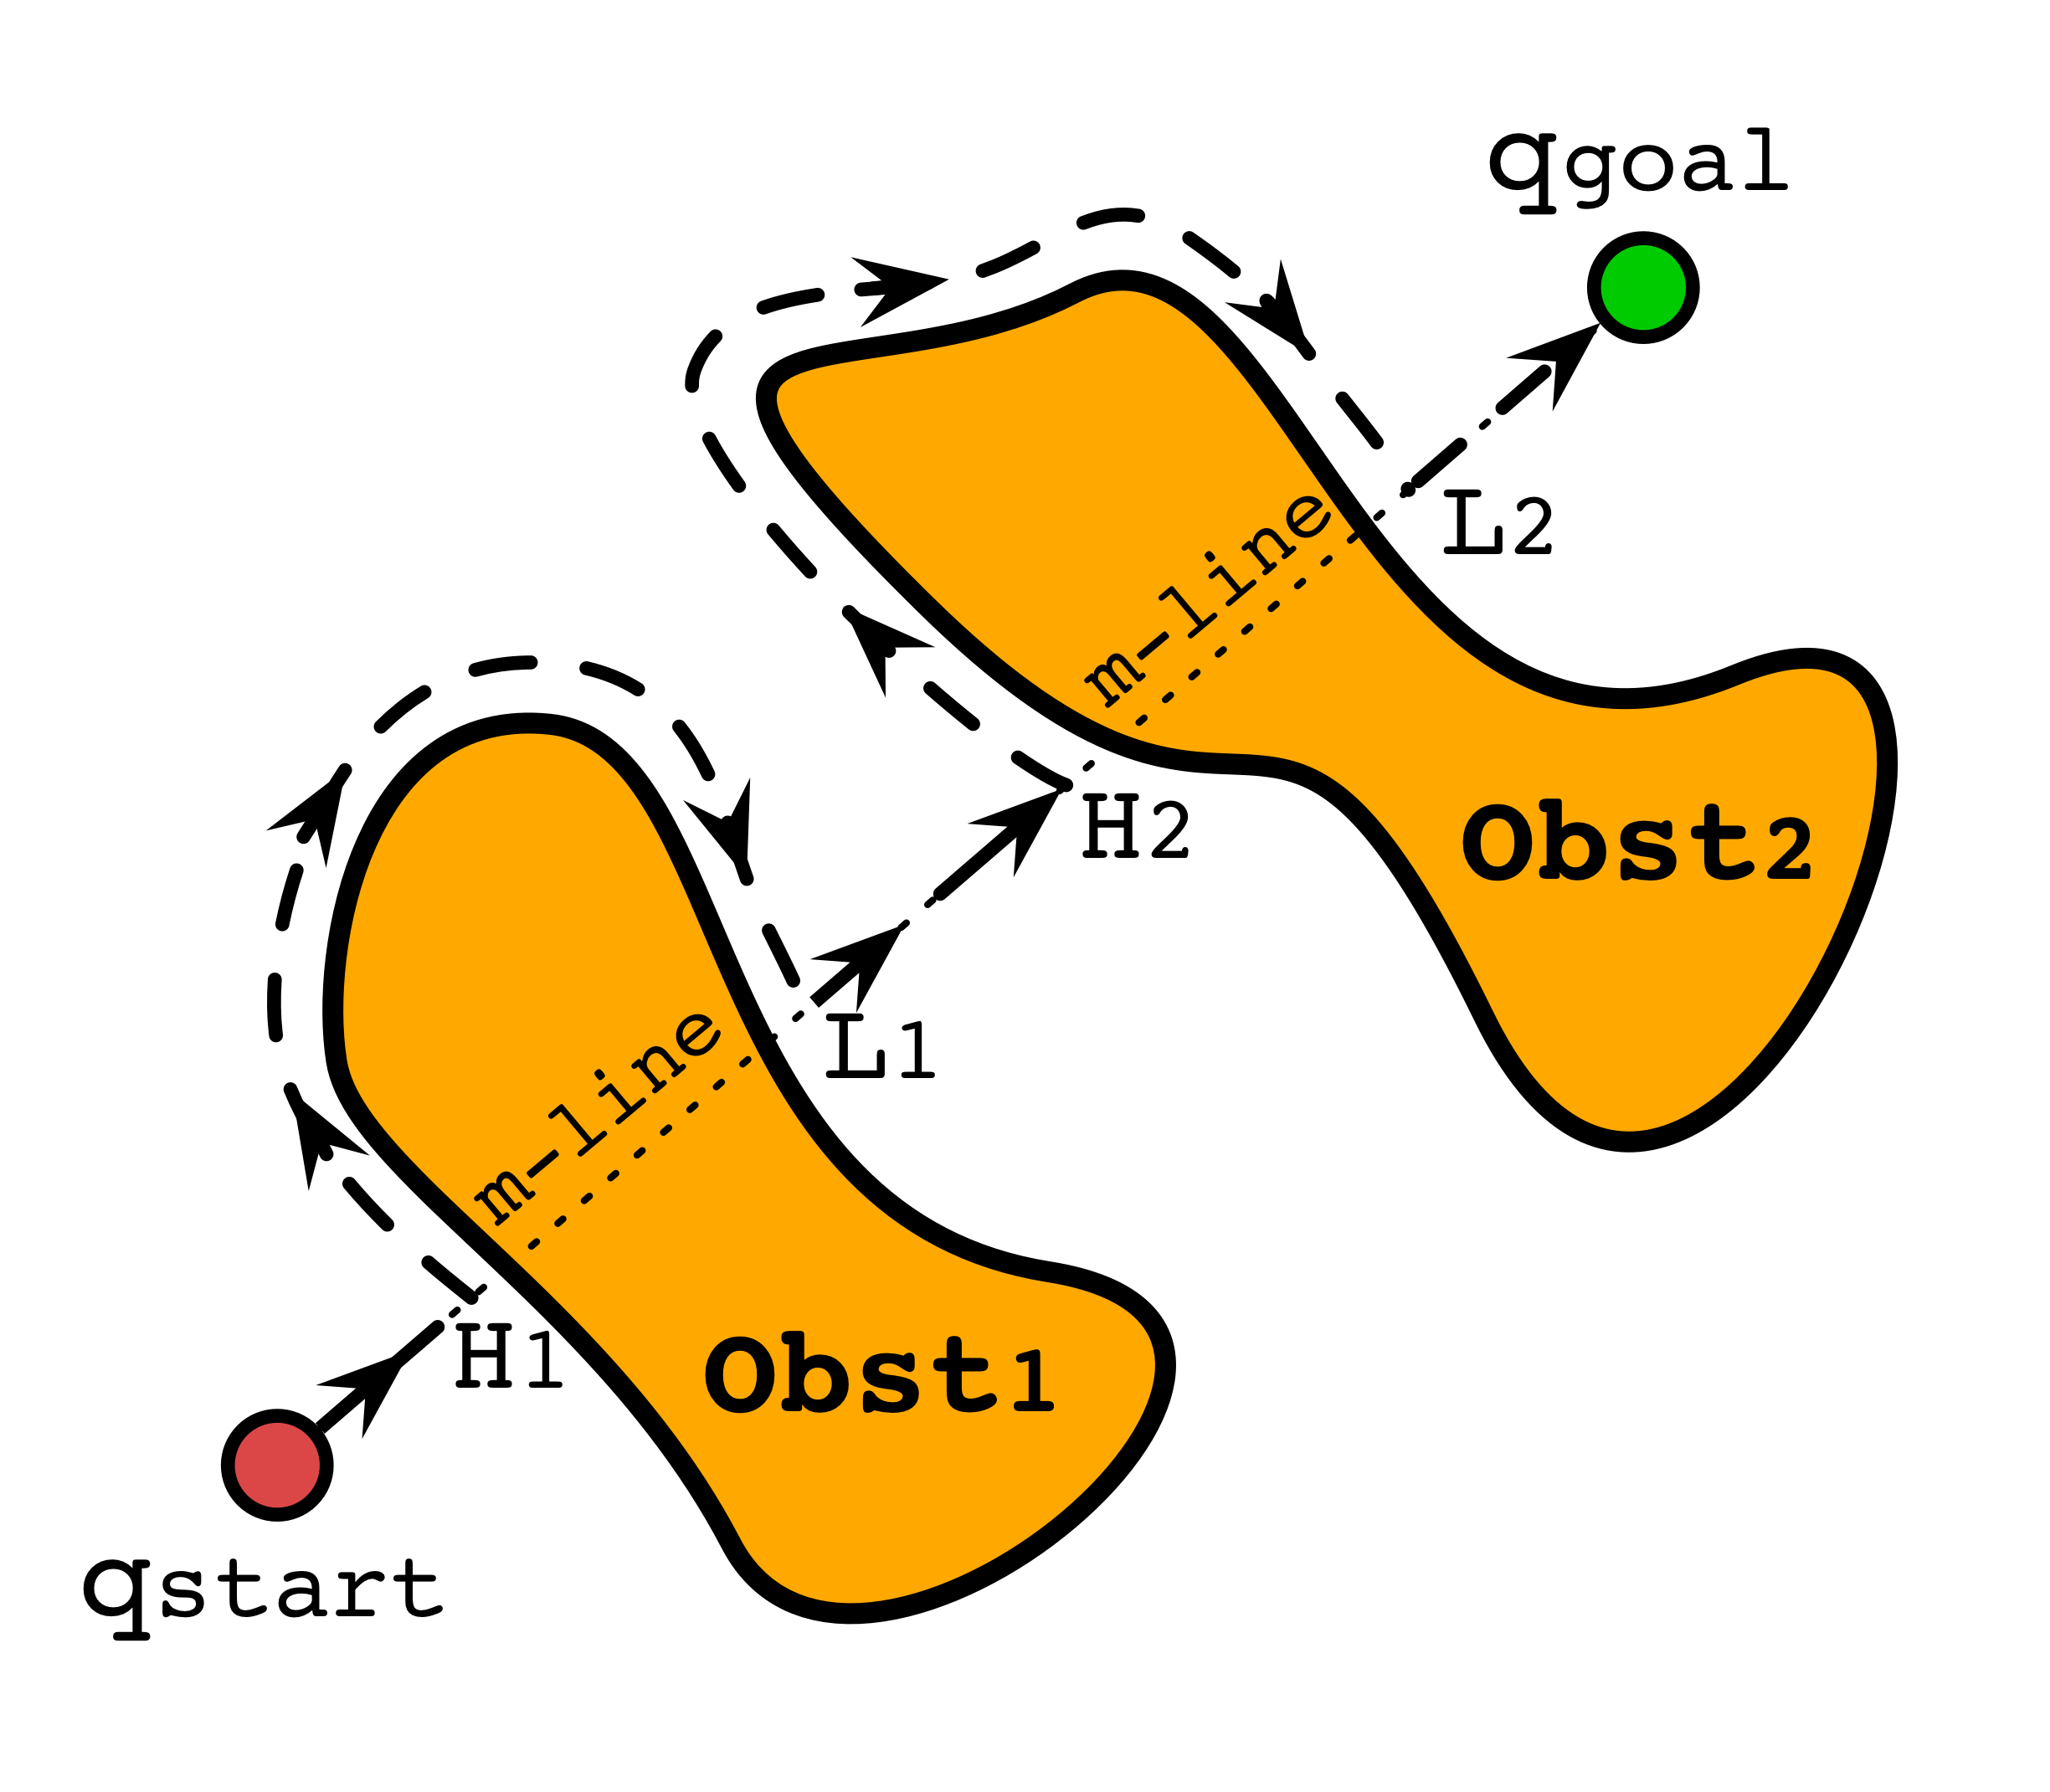
\includegraphics[width=.48\linewidth]{Bug2}} \quad
    \subfloat[Bug2 complex scenario]
    {\label{fig:Bug2-complex}%
     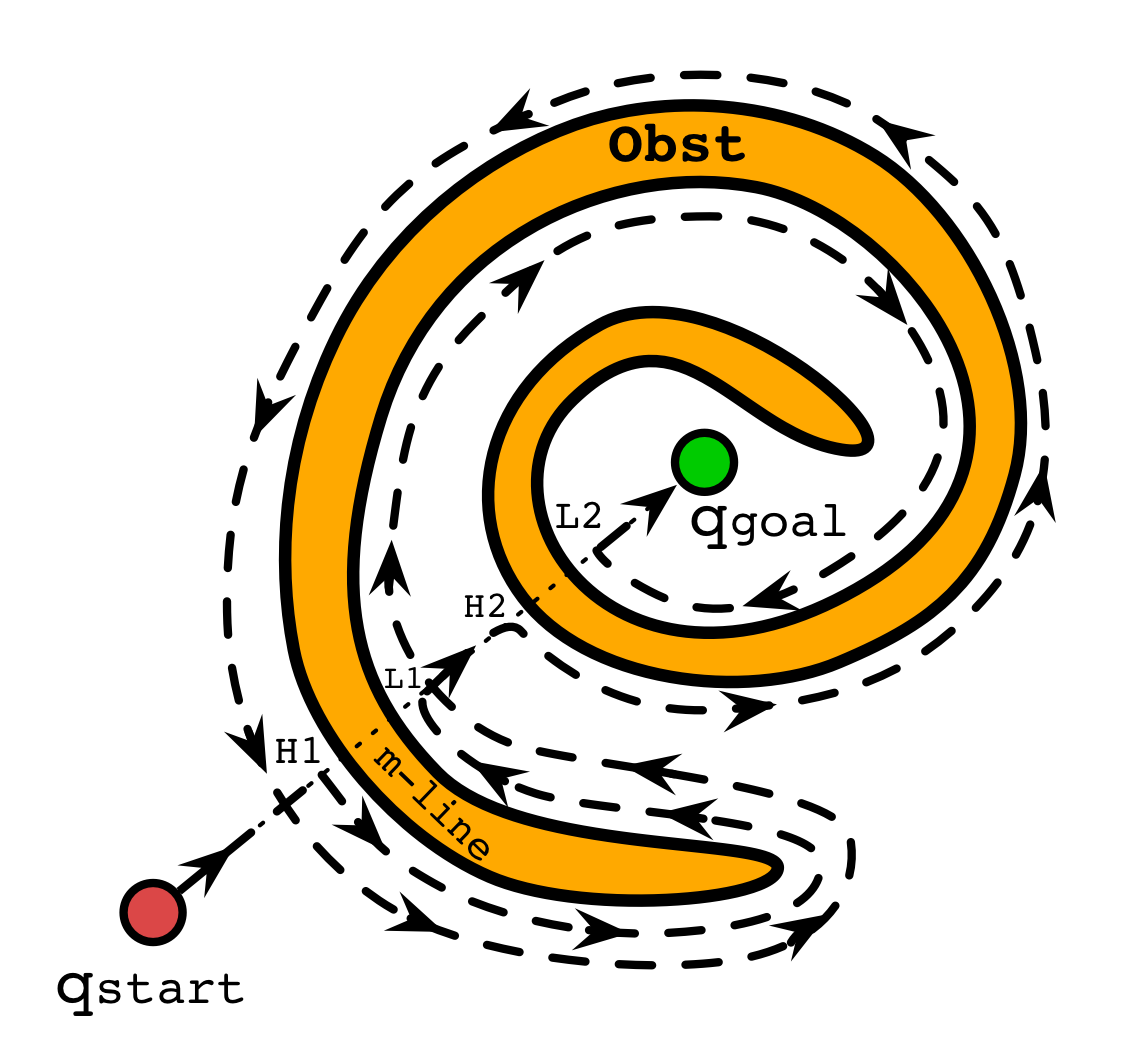
\includegraphics[width=.48\linewidth]{Bug2-complex}}
\caption[Reactive and sensor-based method Bug2.]
{Reactive and sensor-based method Bug2}
\label{fig:Bug2}
\end{figure}
 
Finally, the Tangent Bug algorithm~\cite{Kamon1996} was proposed as an improved
alternative for Bug1 and Bug2. In this version, the robot is assumed to be
equipped with a non-zero range sensor, which permits detecting in advance not
only the obstacles, but also their continuous boundaries. This way, when the
robot is navigating towards the goal and faces an obstacle, it can determine the
discontinuities in the boundaries or the limits of the perceived area, which are
marked as \textit{endpoints}. Then, in order to avoid the obstacle, the robot
checks which of the \textit{endpoints} minimizes the distance to the goal and
starts moving towards it. The procedure is repeated until the obstacle is no
longer perceived, at which point the robot can continue moving towards the goal
following a straight line. Figure~\ref{fig:TangentBug} depicts an example of
Tangent Bug solving a start-to-goal query.
 
\begin{figure}[htbp]
    \myfloatalign
    \subfloat[Boundaries detection]
    {\label{fig:TangentBug-Boundaries}
    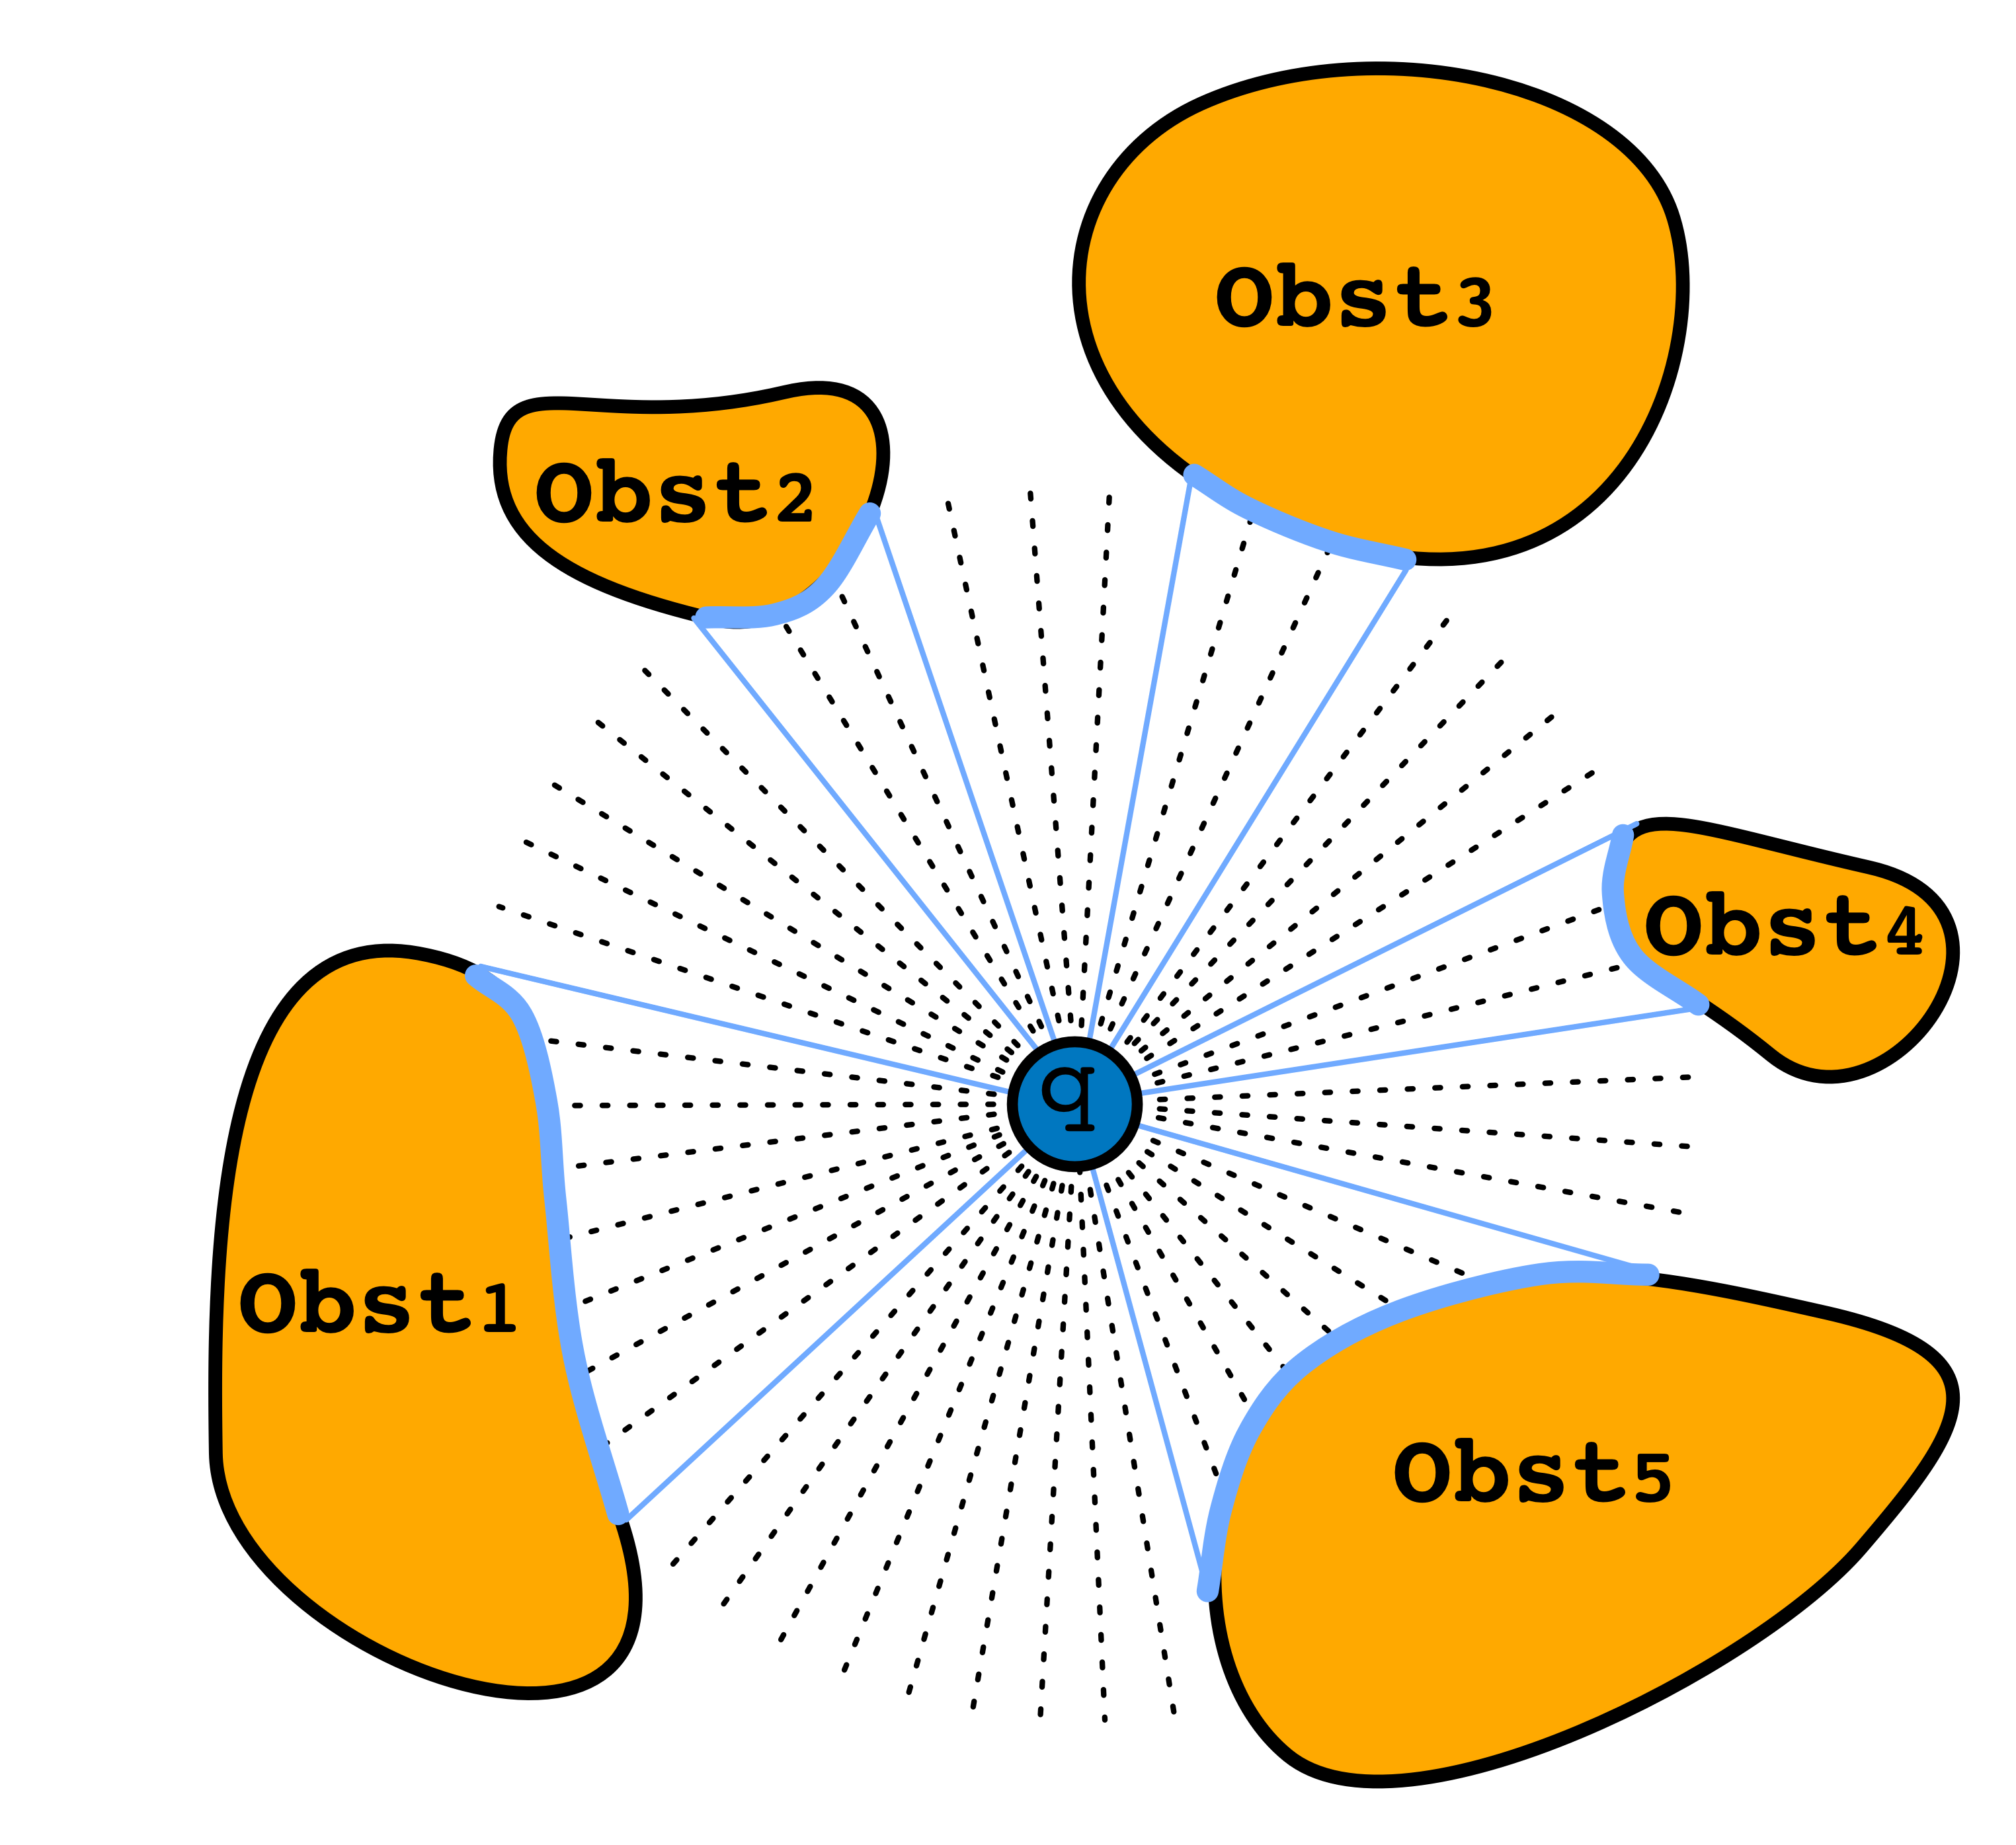
\includegraphics[width=.48\linewidth]{TangentBug-Boundaries}} \quad
    \subfloat[Execution]
    {\label{fig:TangentBug-Execution}%
     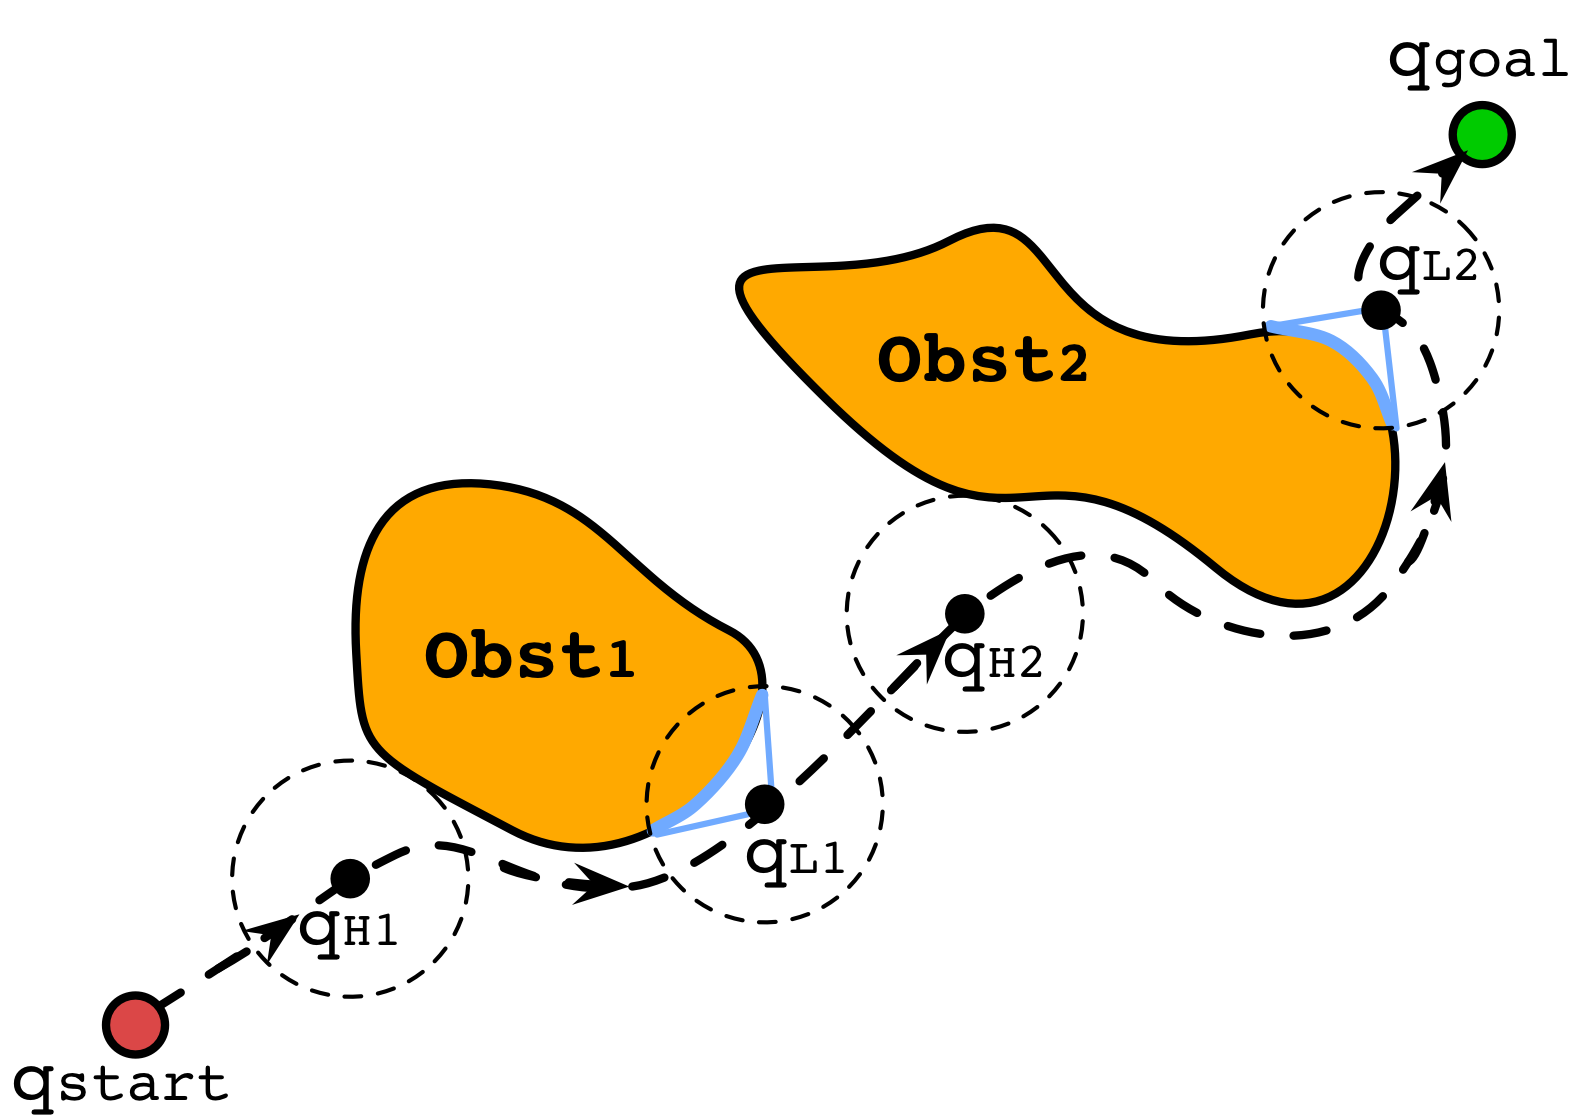
\includegraphics[width=.48\linewidth]{TangentBug-Execution}}
\caption[Reactive and sensor-based method Tangent Bug.]
{Reactive and sensor-based method Tangent Bug}
\label{fig:TangentBug}
\end{figure}

% ----------------------- another section  ------------------------=
\section{Search-based (Grid-based) Path/Motion Planning}
\label{sec:SearchBased}

Search-based planning is a path/motion planning approach that utilizes graph
search methods to find collision-free paths over a discrete version of $\mathcal{C}$.
For doing so, these methods overlay a grid on $\mathcal{C}$ and assume that each
collision-free configuration corresponds to a point on the grid, which is why
they are also called grid-based methods. Over that grid, the robot is allowed to
move from one point to any other adjacent point as long as the line between them
is proved to be collision-free (\ie is contained within $\mathcal{C}_{free}$).
Hence, using this approach to solve, for instance, a start-to-goal query
requires coping with two problems: how to correctly discretize $\mathcal{C}$ to
establish the grid, and how to search a path from the start point to the goal
point (configuration) over such a grid.

For the first problem, it is important to correctly define the grid resolution,
which mainly depends on the environment and the problem's requirements. Coarser
grids, for example, will permit faster searches, but may fail to find paths when
dealing with narrow passages in $\mathcal{C}_{free}$ (see
Figure~\ref{fig:Grid-based}). Finner grids, on the other hand, will allow
solving queries in more complex scenarios, but may be computationally too
expensive for online applications. Once the grid is established, there are
different methods to calculate an optimal path, some of which are described in
this section.

\begin{figure}[htbp]
    \myfloatalign
    \subfloat[Coarse grid]
    {\label{fig:Grid-BasedNarrowPassagesNoValid}%
     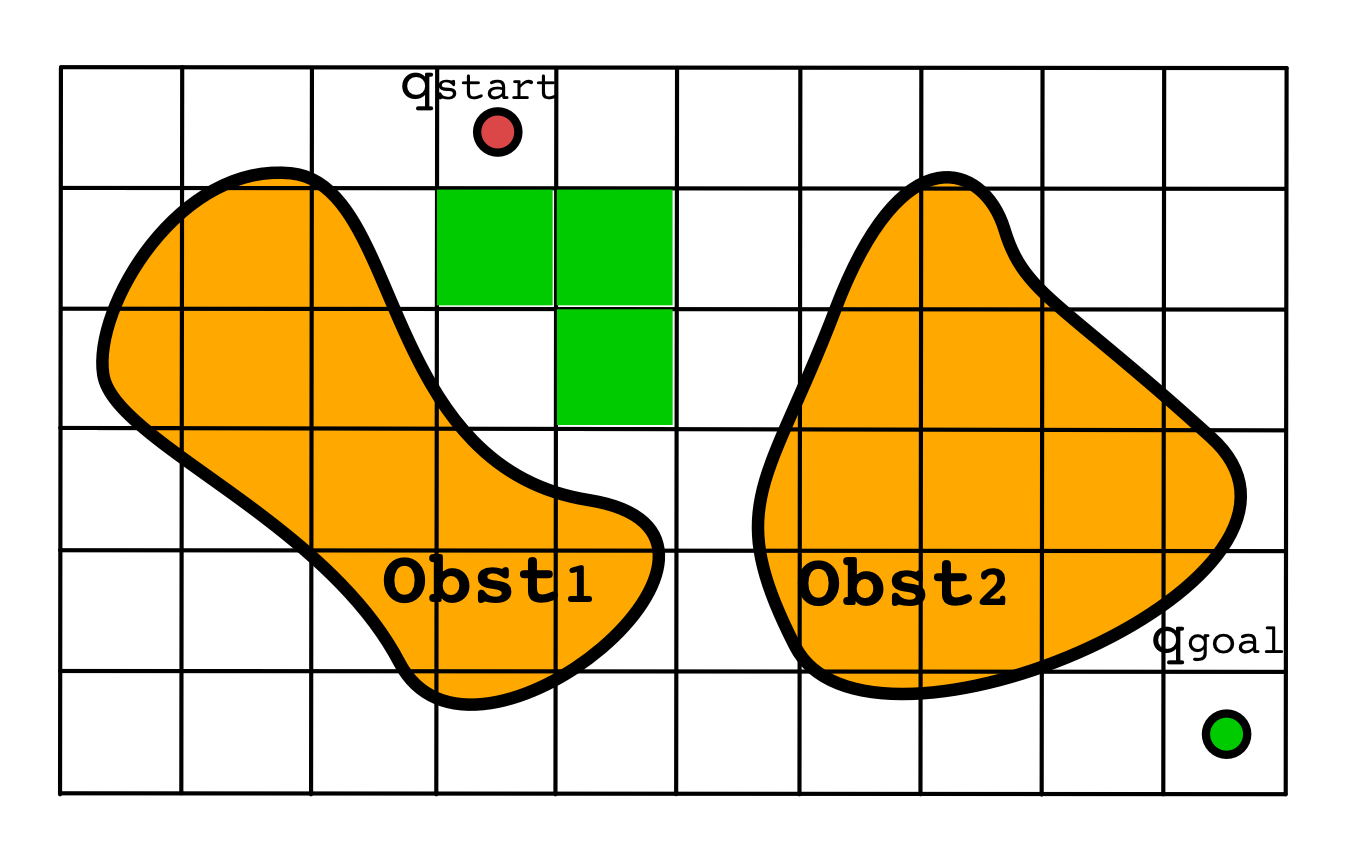
\includegraphics[width=.48\linewidth]{Grid-BasedNarrowPassagesNoValid}} \quad
    \subfloat[Fine grid]
    {\label{fig:Grid-BasedNarrowPassagesValid}
    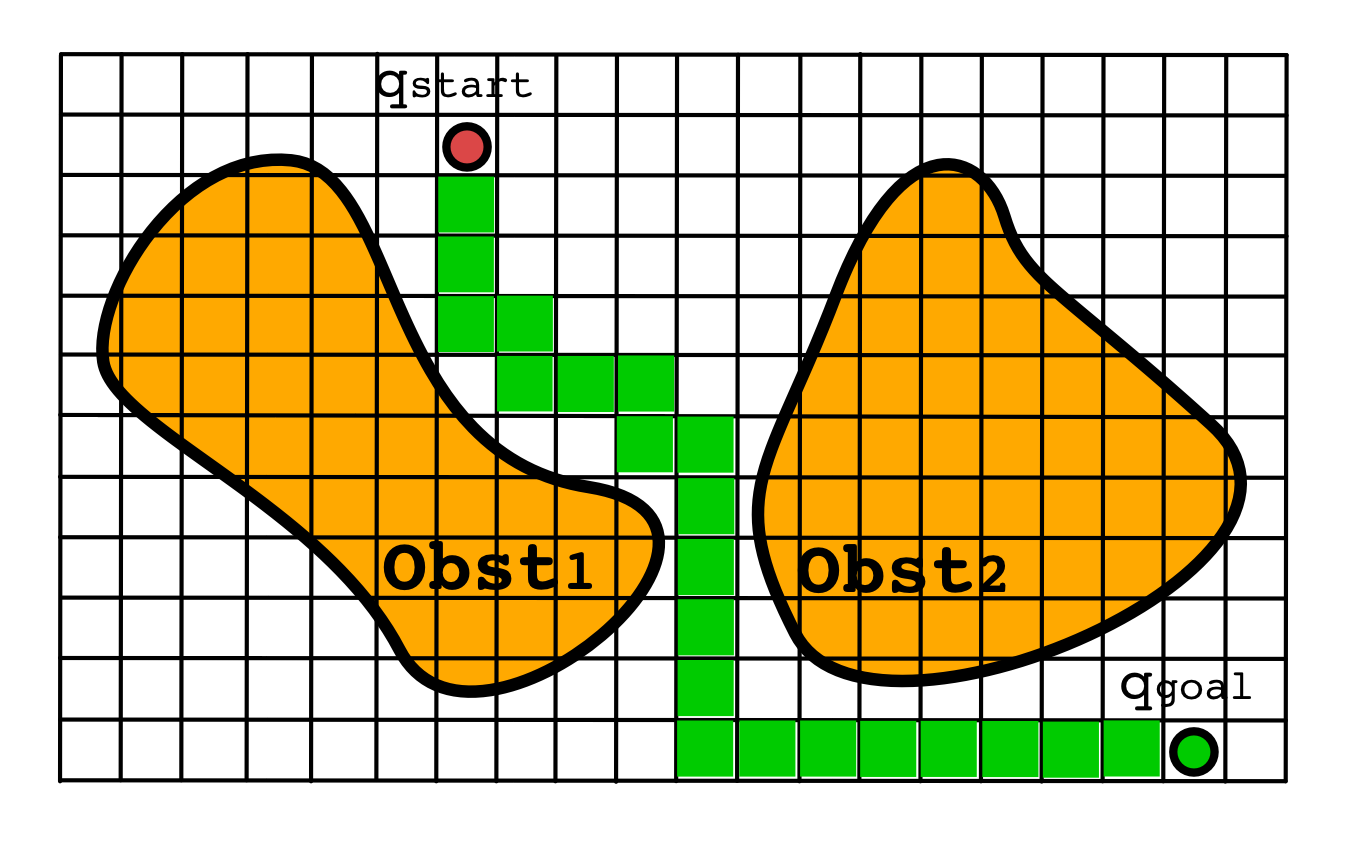
\includegraphics[width=.48\linewidth]{Grid-BasedNarrowPassagesValid}}
\caption[Grid-based method: coarse and fine grid.]
{Grid-based method solving a start-to-goal query.
\protect \subref{fig:Grid-BasedNarrowPassagesNoValid} Although coarser grids
decrease the computing time, they may fail when dealing with narrow passages
where finer grids could succeed \protect
\subref{fig:Grid-BasedNarrowPassagesValid}.}
\label{fig:Grid-based}
\end{figure}

\subsection{Dijkstra's Algorithm}

Presented in 1959, Dijkstra's algorithm~\cite{Dijkstra1959} is one of the first
widely known methods used to find a path in a graph from one node to another.
The algorithm uses a weighted graph $\mathcal{Q}$\footnote{A weighted graph is
one in which numerical values, or weights, are assigned to its nodes and edges.}
to determine which path that connects two nodes has of the lowest cost. While
this method has been used in different areas and applications such as network
routing protocols, in robotics it has been applied to path/motion planning
problems.
There, the associated edge cost may correspond to different optimization metrics
such as distance, energy, time, etc., that can be considered when calculating
the optimal path for a start-to-goal query.

In order to find the optimal path, the algorithm iteratively executes the
following steps until reaching the goal ($q_{goal}$):
\begin{inparaenum}[1)] \item Setting an initial cost to all nodes, specifically
zero to the initial one ($q_{start}$) and infinity to all others.
\item Establishing $q_{start}$ as the current node and marking the rest as
unvisited.
\item Calculating the cost for the current node's unvisited neighbors (equal to
the current node's cost plus the edge to the neighbor cost), as well as updating
any previously calculated node cost if the new value is lower.
For example, if node $B$ cost was $x$ when current node was $A$, but the new
cost is $y$ when current node is $C$, and $y<x$, then node $B$ cost will be now
$y$.
\item After calculating the cost of all its unvisited neighbors, current
node is marked as visited.
\item If the $q_{goal}$ has been marked as visited, the algorithm has finished,
otherwise, the new current node will be the unvisited node with the lowest
cost, and will be processed as indicated from step 3).
\end{inparaenum}
Finally, the least cost path can be obtained with backtracking.
Figure~\ref{fig:Dijkstra} presents an example of executing this method.

\subsection{A*}

In 1968, Peter Hart \etal described an extension of Dijkstra's algorithm called
A*~\cite{Hart1968}, which incorporates a heuristic that permits estimating the
cost of paths from any node of the graph to the goal. Because of this
characteristic, A* is considered an informed search algorithm; this means that
it always attempts to find the path by firstly evaluating those nodes with the
minimum estimated cost according to the heuristic. As occurs with Dijkstra's
algorithm, A* starts from a weighted graph $\mathcal{Q}$, in which each node
represents a different configuration contained in $\mathcal{C}_{free}$ and the
edges correspond to collision-free paths between configurations. Then, it builds
a search tree, rooted at $q_{start}$, by expanding different paths, one step at
a time, until one of them ends at the desired $q_{goal}$. The main difference
with respect to Dijkstra's algorithm is the order in which each partial path is
expanded. In the case of A*, it expands the node $q_i$ that minimizes the total
cost $f(q_i) = g(q_i) + h(q_i)$, which combines the cost required to reach the
node from the start configuration $g(q_i)$ with the estimated heuristic cost
from the node to the goal $h(q_i)$.

While both Dijkstra's algorithm and A* can generate optimal solutions, the
latter can result in a more efficient search by reducing the number of nodes
required to be visited in order to determine the solution path (see
Figure~\ref{fig:Astar}). However, it is important to know that an
incorrect heuristic will also provide a valid solution, but it may be
suboptimal. For this reason and in order to produce an optimal path, the
heuristic has to be optimistic, or admissible, which means that the estimated
cost to the goal has to be lower or equal to the real cost~\cite{Choset2005}.
Finally, it is also important to note that in case no heuristic is provided, \ie
$h(q_i)=0$, A* behaves as Dijkstra's algorithm. Algorithm~\ref{alg:A-star}
presents the pseudocode for A* and also provides a general idea for Dijkstra's
algorithm explained in the previous section.

\begin{figure}[htbp]
    \myfloatalign
    \subfloat[Dijkstra algorithm]
    {\label{fig:Dijkstra}%
     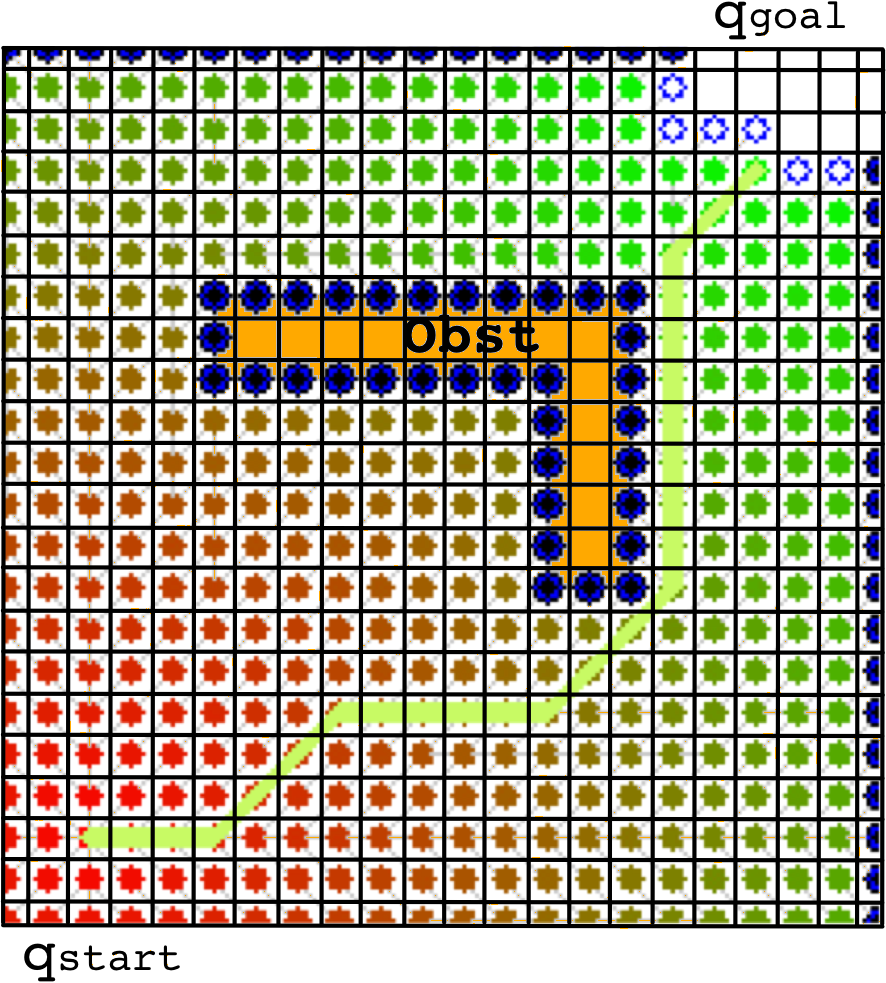
\includegraphics[width=.48\linewidth]{Dijkstra}} \quad
    \subfloat[A*]
    {\label{fig:Astar}
    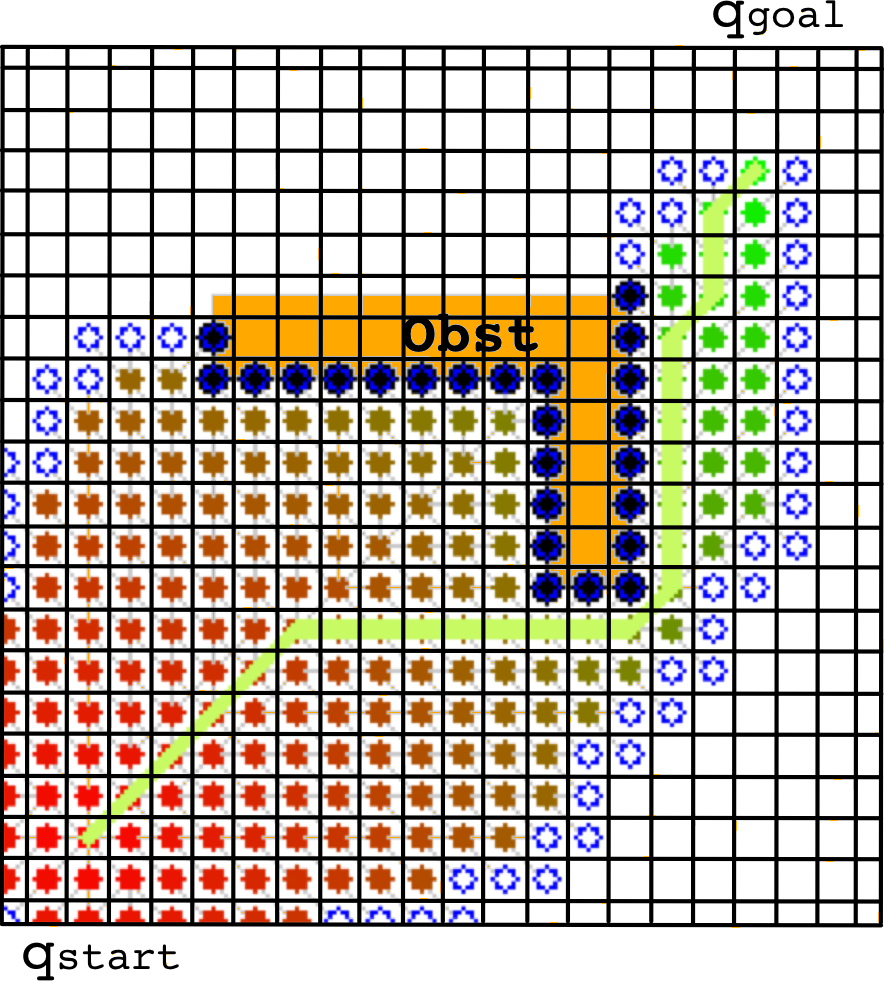
\includegraphics[width=.48\linewidth]{Astar}}
\caption[Comparison between Dijkstra's algorithm and A*.]
{Grid-based methods solving a start-to-goal query.
\protect \subref{fig:Dijkstra} Dijkstra's algorithm requires an exhaustive
search to determine the shortest path to the goal.
\protect \subref{fig:Astar} A* requires exploring less cells since it uses a
heuristic to guide the search. Image credit: modified from Wikipedia.}
\label{fig:Dijkstra-Astar}
\end{figure}

\begin{algorithm}[htbp]
	\DontPrintSemicolon
	\SetKwFunction{popWithMinCost}{popWithMinCost}
	\SetKwFunction{PriorityQueue}{PriorityQueue}
	\SetKwFunction{insertQ}{insert}
	\SetKwFunction{Neighbors}{Neighbors}

	\KwIn{\\ 
	$q_{start}$: Start configuration.\\
	$q_{goal}$: Goal configuration.\\
	$\mathcal{Q}$: Graph of configurations $q$, such that $q \in \mathcal{C}_{free}$}

 	\Begin{
 		\ForAll{$q \in \mathcal{Q}$}{
 			$g(q) = \infty$\;
 		}
 		$g(q_{start}) = 0$\\
 		UNVISITED = \PriorityQueue{}\\
 		UNVISITED.\insertQ{$q_{start}$, $g(q_{start})+h(q_{start}, q_{goal})$}\\
 		\While{$\argmin\limits_{q \in UNVISITED} (g(q)+h(q, q_{goal})) \neq
 		q_{goal}$}{
 			$q \leftarrow$UNVISITED.\popWithMinCost{}\\
 			\ForAll{$q' \in \mathcal{Q}.\Neighbors{q}$}{
	 			\If{$g(q')>g(q)+c(q,q')$}{
	 				$g(q') = g(q) + c(q,q')$\\
	 				UNVISITED.\insertQ{$q'$, $g(q')+h(q', q_{goal})$}\\
 				}
	 		}
 		}
 	}
 \caption{A*}
 \label{alg:A-star}
\end{algorithm}

\subsection{Dynamic A* (D*)}
\label{sec:D-star}

The aforementioned search-based algorithms, at least in their original versions,
are intended for planning paths in static environments. Nonetheless, there are
situations, especially in mobile robotics applications, in which elements of the
environment may change. For those cases, Anthony Stentz proposed the
\ac{D*}~\cite{Stentz1994,Stentz1995}, an incremental search-based algorithm that
plans collision-free paths using a similar strategy as A*. The difference is
that it also allows to replan according to changes observed in the surroundings
while the robot follows the path to the goal. Its most important characteristic
is that it locally repairs the path, which is more efficient that invoking
multiple times A* to find a new valid path. Contrary to Dijkstra's algorithm and
A*, that both search paths from the start to the goal configuration, \ac{D*}
expands nodes by searching backwards from the goal until the node to be expanded
coincides with the start configuration, at which time the search is concluded.
At the moment, \ac{D*} and some of its variants are probably the most used
search-based methods in mobile robotics. Some of those extensions and
applications will be presented in Section~\ref{sec:ExtensionsApplications}.

% ----------------------- another section  ------------------------
\section{Potential Fields}
\label{sec:PotenFields}

Even though search-based methods have proved to be successful in \ac{2D} and
\ac{3D} workspaces for some terrestrial, aerial and even aquatic robotic
applications, those exhaustive methods suffer from scalability issues in
problems involving high-dimensional configuration spaces. Another important
drawback is the necessity of establishing a grid over $\mathcal{C}_{free}$,
which means discretizing the \ac{C-Space}, thus limiting the possible and
available solutions according to the chosen resolution. An alternative approach
is the use of potential functions.

Originally proposed by Oussama Khatib in 1985~\cite{Khatib1985,Khatib1986},
potential functions, also known as \textit{potential fields}, constitute a
reactive approach for path/motion planning, which attempts to guide a robot from
an initial configuration to a goal configuration while avoiding obstacles. A
\textit{potential field} basically defines a real-valued function $U:
\mathbb{R}^m \rightarrow \mathbb{R}$, which is composed of an attractive
component $U_a(q)$ that pulls the robot towards the goal, and a repulsive
component $U_r(q)$ that pushes the robot away from the obstacles. This function
can be viewed as the total energy $U(q) = U_a(q) + U_r(q)$, which means that the
total force applied by the potential field to the robot is defined as the
negative of the vector gradient, \ie $f(q) = -\nabla U(q)$, where $\nabla U(q) =
DU(q)^T = \left[ \frac{\partial U}{\partial q_1}(q), \ldots, \frac{\partial
U}{\partial q_m}(q) \right]^T$. In other words, the gradient $\nabla U(q)$
establishes the force required at any $q \in \mathcal{C}$, in order to guide the
robot throughout a collision-free path towards the goal.
Figure~\ref{fig:potential-field} presents an example of the two components of a
potential field and the total potential field.


\begin{figure}[htbp]
    \myfloatalign
    \subfloat[Top view]
    {\label{fig:PotentialFieldTop}%
     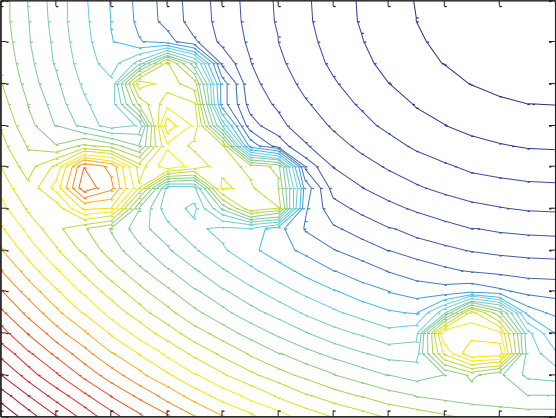
\includegraphics[width=.48\linewidth]{PotentialFieldTop}} \quad
    \subfloat[Perspective view]
    {\label{fig:PotentialFieldPerspective}
    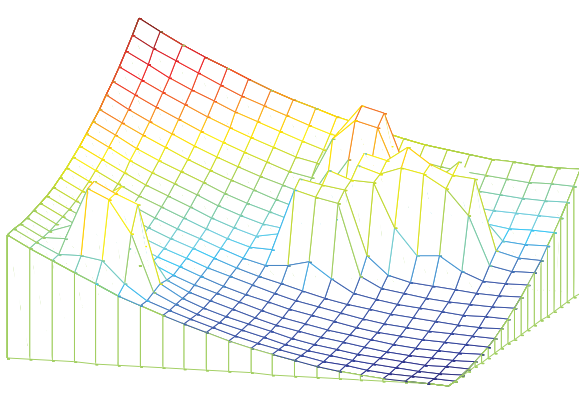
\includegraphics[width=.48\linewidth]{PotentialFieldPerspective}}
\caption[Example of potential field.]
{Example of potential field. The obstacles can be observed as a repulsive
component of the whole potential. Image credit: Liu \etal\cite{Liu2016}.}
\label{fig:potential-field}
\end{figure}

Once the potential function and the corresponding gradient have been
established, the solution path to a start-to-goal query can be incrementally
obtained by using the gradient descent, which is a widely-known algorithm in
solving optimization problems. Having $q_{start}$ as the initial configuration,
the algorithm iteratively calculates a new configuration by moving in the
direction opposite to the gradient until the gradient is zero. The pseudocode
for this method is presented in Algorithm~\ref{alg:Gradient-descent}.

\begin{algorithm}[htbp]
	\DontPrintSemicolon

	\KwIn{\\ 
	$q_{start}$: Start configuration.\\
	$\nabla U(q)$: Gradient of the potential field.}

 	\Begin{
 		$q(0) = q_{start}$\\
 		$i = 0$\\
 		\While{$\nabla U(q(i)) \neq 0$}{
 			$q(i + 1) = q(i) - \nabla U(q(i))$\\
 			$i = i + 1$
 		}
 	}
 \caption{Gradient Descent}
 \label{alg:Gradient-descent}
\end{algorithm}

However, the gradient descent algorithm using potential functions as explained
above does not guarantee finding or converging to a solution for a start-to-goal
query. This happens because it may reach a local minimum of $U(q)$ that may not
correspond to $q_{goal}$. To deal with such situations, Barraquand and Latombe
proposed the \ac{RPP}~\cite{Barraquand1990, Barraquand1991}, which is an
algorithm that makes use of the gradient descent together with random walks and
backtracking in order to avoid issues related to local minima. However, it is
important to note that \ac{RPP} effectiveness is highly dependent on parameter
tuning. Another important aspect to highlight is that \ac{RPP} was one of the
first methods to use a stochastic or random approach for path/motion planning;
algorithms with this characteristic will be discussed more in detail in
Section~\ref{sec:SamplingBasedAlg}.

% ----------------------- another section  ------------------------
\section{Roadmaps}
\label{sec:Roadmaps}

So far, the methods and algorithms presented above attempt to solve a single
start-to-goal query, which means they calculate a path that connects a start
configuration and a goal configuration. For doing so, they incrementally search
a path towards the goal while avoiding, at the same time, collisions with the
obstacles. Nonetheless, there are some applications in which the path/motion
planner is intended to solve more that one query. For those cases, it makes
sense to have a map that contains the information about all feasible routes, and
that can also be used more than once to solve multiple start-to-goal queries.
There are different alternatives to define a map that can be used for
path/motion planning, including topological, geometric, and grid-based
representations.

This section reviews methods that use a class of topological maps called
\textit{roadmaps}~\cite{Canny1993, Latombe1991}. A \ac{RM} is defined as
a subset of the \ac{C-Space} that results from the union of curves, in which any
$q_{start}$ and $q_{goal}$ contained in $\mathcal{C}_{free}$ can be connected by
a path that meets the following properties~\cite{Choset2005}:
\begin{inparaenum}[1)] \item \textbf{Accessibility} - there is a path from
$q_{start}\in\mathcal{C}_{free}$ to some $q'_{start}\in\mathcal{RM}$.
\item \textbf{Departability} - there is a path from some
$q'_{goal}\in\mathcal{RM}$ to $q_{goal}\in\mathcal{C}_{free}$.
\item \textbf{Connectivity} - there is a path in $\mathcal{RM}$ that
connects $q'_{start}$ and $q'_{goal}$.
\end{inparaenum}

\subsection{Visibility Graphs}

Visibility graphs are one of the alternatives in defining a roadmap. Assuming a
\ac{2D} \ac{C-Space} with polygonal obstacles, the set of the visibility graph
nodes ($v_i$) is composed of $q_{start}$, $q_{goal}$, and all the vertices of
the obstacles. Its edges, $e_{ij}$, are straight-line segments that can connect
any possible combination of two nodes $v_i$ and $v_j$, without colliding with
the obstacles ($e_{ij}\in\mathcal{C}_{free}$). Once the visibility graph is
fully defined, the solution path can be obtained by conducting any graph-based
search method, such as those explained in Section~\ref{sec:SearchBased}.
While Figure~\ref{fig:Visibility-Graph} depicts an example of a visibility graph
and a start-to-goal query solution over it, Algorithm~\ref{alg:Visibility-Graph}
presents the pseudocode to build a visibility graph.

\begin{figure}[htbp]
    \myfloatalign
    \subfloat[]
    {\label{fig:VisibilityGraph1}
    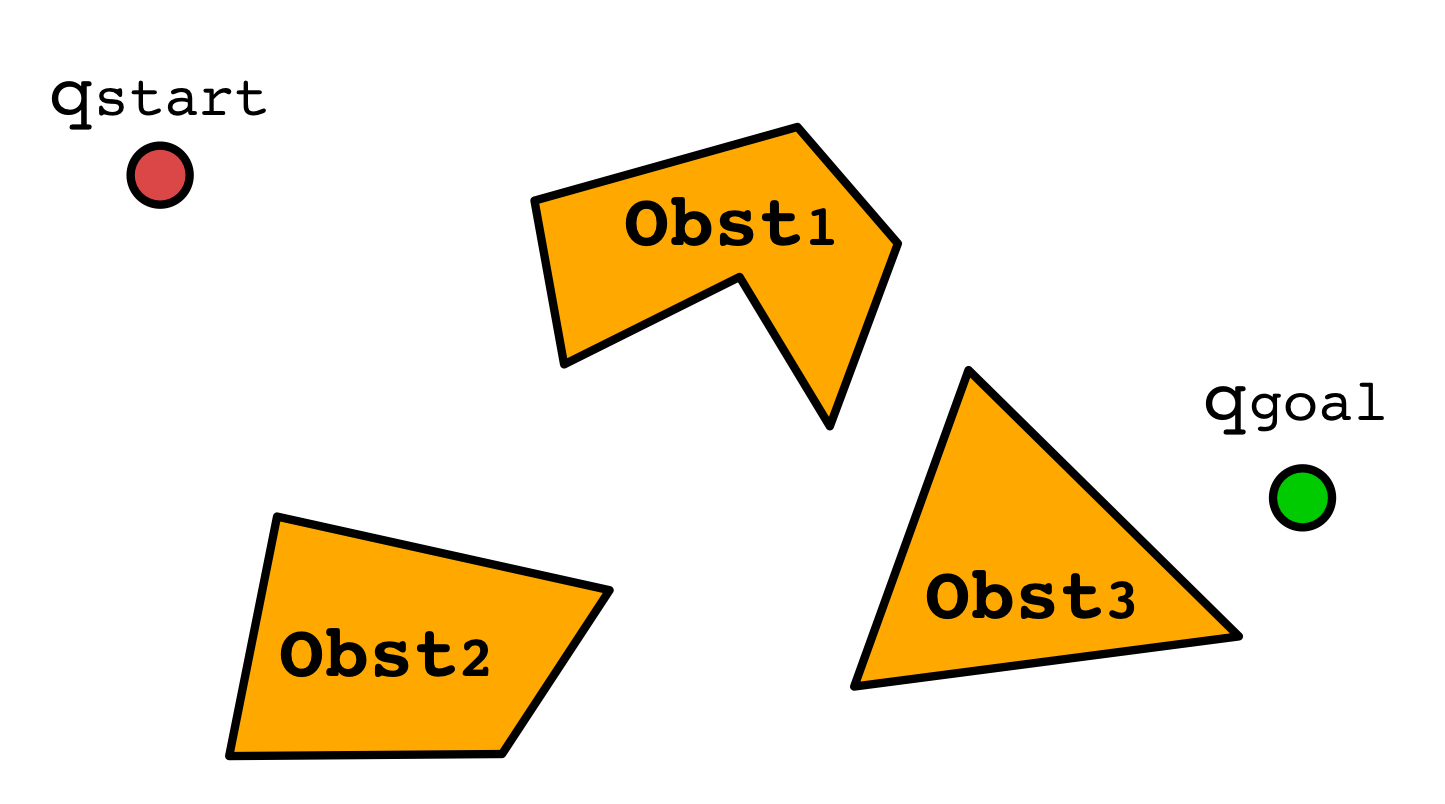
\includegraphics[width=.45\linewidth]{VisibilityGraph1}} \quad
    \subfloat[]
    {\label{fig:VisibilityGraph2}%
     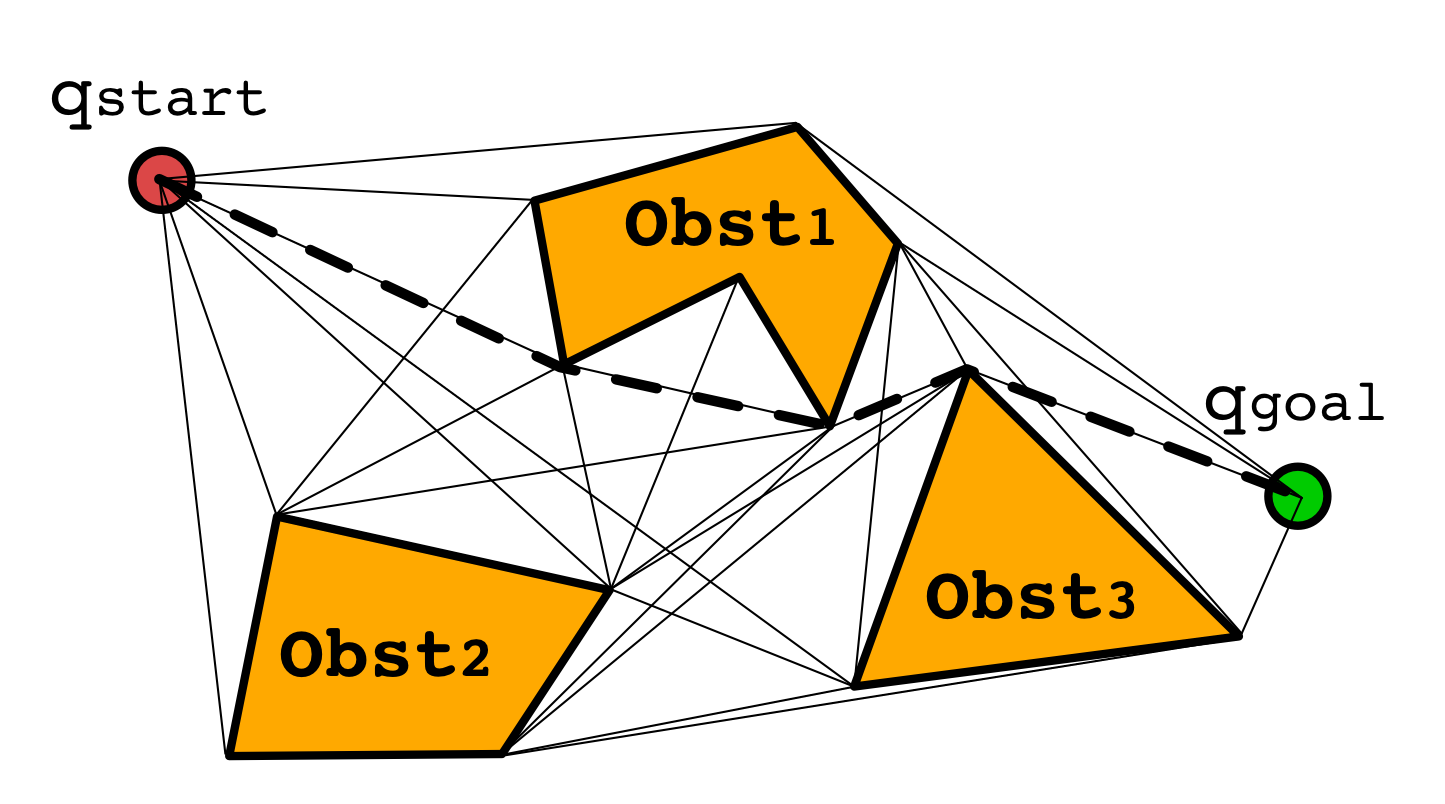
\includegraphics[width=.45\linewidth]{VisibilityGraph2}}
\caption[Example of a visibility graph.]
{Example of a visibility graph.
\protect \subref{fig:VisibilityGraph1} A 2D C-Space that contains polygonal
obstacles, a start configuration, and a goal configuration.
\protect \subref{fig:VisibilityGraph2} A roadmap is built by connecting any
possible combination of two vertices without colliding with the obstacles. The
start-to-goal query is solve using a graph search method.}
\label{fig:Visibility-Graph}
\end{figure}

\begin{algorithm}[htbp]
	\DontPrintSemicolon

	\SetKwFunction{addNodes}{addNodes}
	\SetKwFunction{getVertices}{getVertices}
	\SetKwFunction{getNumNodes}{getNumNodes}
	\SetKwFunction{findStraightLine}{findStraightLine}
	\SetKwFunction{isCollisionFree}{isCollisionFree}
	\SetKwFunction{addEdge}{addEdge}

	\KwIn{\\
	$q_{start}$: Start configuration.\\
	$q_{goal}$: Goal configuration.\\
	World: $n$ Obstacles.}
	
	\KwOut{\\
	Roadmap ($\mathcal{RM}$): Visibility Graph(VG) = $(V, E)$.}
	
	\Begin{
		$V=\{ \, \}$\;
		$E=\{ \, \}$\;
		\For{$ i=1:n$}{
	 		$V$.\addNodes{$Obst(i)$.\getVertices{}}\;
	 	}
	 	
	 	\For{$ i=1:$V$.\getNumNodes{}$}{
	 		\For{$ j=1:$V$.\getNumNodes{}$ and $j\neq i$}{
	 			$v_i\leftarrow$ $V(i)$\;
	 			$v_j\leftarrow$ $V(j)$\;
	 			$e_{ij}\leftarrow$ \findStraightLine{$v_i,v_j$}\;
	 			\If{\isCollisionFree{$e_{ij}$}}{
	 				$E$.\addEdge{$e_{ij}$}\;
 				}
	 		}
	 	}
 	}
 \caption{Visibility Graph}
 \label{alg:Visibility-Graph}
\end{algorithm}

\subsection{Generalized Voronoi Diagrams}

Another alternative to build a roadmap for path/motion planning is the \ac{GVD}.
The \ac{GVD} is defined for a set of points called \textit{sites}; given a
particular site, the set of points closest to it is called a \textit{Voronoi
region}. Finally, the Voronoi diagram is the set of points that are equidistant
to at least two sites~\cite{Aurenhammer1991}. In path/motion planning
applications, the \ac{GVD} defines the sets of points equidistant to at least
two obstacles. This means that the sites are the center of the obstacles to be
avoided, and the edges correspond to the possible channels that maximize the
distance to the obstacles~\cite{Choset2005}. Figure~\ref{fig:VoronoiDiagram}
displays an example of a planar \ac{GVD}.

\begin{figure}[htbp]
	\centering
	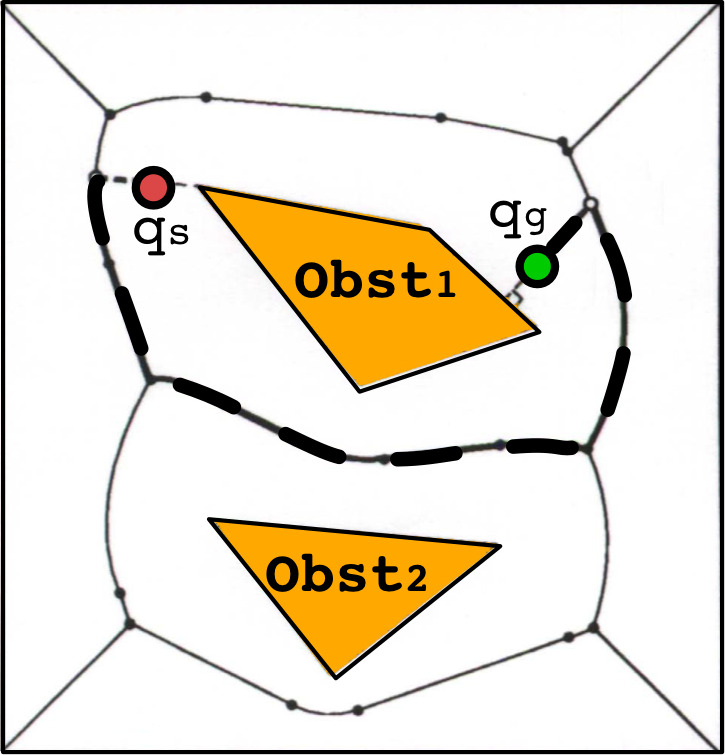
\includegraphics[width=.35\linewidth]{VoronoiDiagram}
\caption[Example of a voronoi diagram.]
{Example of a Voronoi diagram}	
\label{fig:VoronoiDiagram}
\end{figure}

% ----------------------- another section  ------------------------
% \section{Cell Decomposition}
% 
% Resolution completeness ?

%  \hl{Next, we consider a different type of representation of the free space
%  called an exact cell decomposition. These structures represent the free space by the union
% of simple regions called cells. The shared boundaries of cells often have a
% physical meaning such as a change in the closest obstacle or a change in line of
% sight to surrounding obstacles. Two cells are adjacent if they share a common
% boundary. An adjacency graph, as its name suggests, encodes the adjacency
% relationships of the cells, where a node corresponds to a cell and an edge
% connects nodes of adjacent cells.
% 
% Assuming the decomposition is computed, path planning with a cell decomposition
% is usually done in two steps: first, the planner determines the cells that
% contain the start and goal, respectively, and then the planner searches for a
% path within the adjacency graph. Note that the adjacency graph could serve as a
% roadmap of the free space as well. Therefore, mapping can be achieved by
% incrementally constructing the adjacency graph.
% 
% Cell decompositions, however, distinguish themselves from other methods in that
% they can be used to achieve coverage. A coverage path planner determines a path
% that passes an effector (e.g., a robot, a detector, etc.) over all points in a
% free space. Since each cell has a simple structure, each cell can be covered
% with simple motions such as back-and-forth farming maneuvers; once the robot
% visits each cell, coverage is achieved. In other words, coverage can be reduced
% to finding an exhaustive walk through the adjacency graph. Sensor-based coverage
% is achieved by simultaneously covering an unknown space and constructing its
% adjacency graph.
% 
% The most popular cell decomposition is the trapezoidal decomposition [356]. This
% decomposition relies heavily on the polygonal representation of the planar
% configuration space. A more general class of decompositions, which are termed
% Morse Decompositions [12], allow for representations of nonpolygonal and
% nonplanar spaces. Morse decompositions are based on ideas from Canny's roadmap
% work. We then consider a broader class of decompositions which includes those
% based on visibility constraints. One such decomposition serves as a basis for
% the pursuit/evasion problem which is introduced section 6.3. [Choset]
% 
% Cell decomposition refers to any method that partitions the free configuration
% space into a set of smaller cells [49]. Once the decompostion has been done, a
% connectivity graph can be built, where the cells are the nodes, and cells that
% share a common edge are connected in the graph. 
% 
% Cell decompositions are classified as either exact, semi-approximate, or
% approximate [49]. Within the cell decomposition methods, the major differences
% are generally based on how to generate the cells and what shape they should be.
% Pioneering work in this field was done by Acar and Choset. The Boustophedeon
% cell decomposition is first introduced in [48] and is based on previous work by
% Canny and Lin [43]. The cell decomposition is generated by determining critical
% points in the workspace where the connectivity of a slice, or 1-D line, of the
% free space changes as it is swept across the workspace. This is expanded in [1,
% 2] to include a method in which critical points can be detected online and the
% decomposition is referred to as a Morse decomposition. The connectivity of the
% cells is represented by the Reeb graph. In [3], the approach is applied to a
% terrestrial demining task where the robot is able to detect and exploit the
% pattern of the mines to search more efficiently. In [4], the algorithm is
% extended to apply to a robot whose sensor swath is larger than the platform
% footprint. In this approach, two heuristics are combined: one for coverage of
% wide open spaces based on Boustrophedon search, and one for constricted areas
% which is based on the GVD. 
% 
% Once the cell decomposition is made, a graph is generated where each cell
% represents a node in the tree and adjacent cells are connected with an edge. As
% mentioned, this type of decomposition is most useful for achieving coverage, but
% start-to-goal planning can be done by reducing each cell to one or a few points.
% In Fig. 2.10 each cell has been reduced to its centroid. The centroids of cells
% in the figure are denote by black dots. The blue lines represent the critical
% slices. Note that every critical slice is tangent to an obstacle but cannot
% penetrate an obstacle. As per the earlier figures, the obstacles are shown in
% red. The path found by connecting centroids is shown as the yellow line. Note
% that in this simplistic case, a suboptimal path is generated because of the
% reduction of the cells to only their centroids. [Paull13]}

% \begin{figure}[htbp]
% 	\centering
% 	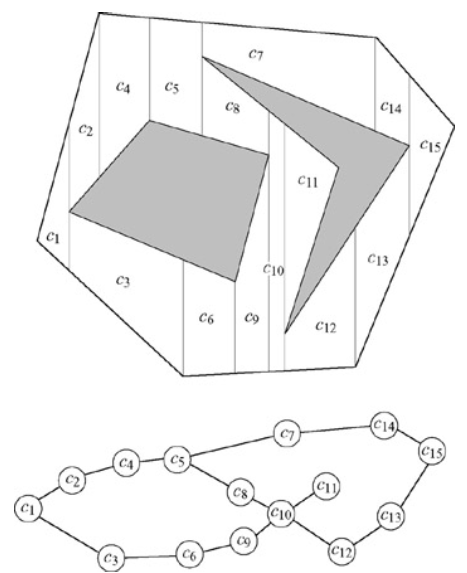
\includegraphics[width=.45\linewidth]{Cell-Decomposition} \quad
% 	\caption{\hl{Cell-Decomposition}}
% 	\label{fig:Cell-Decomposition}
% \end{figure}

% ----------------------- another section  ------------------------
\section{Sampling-based Algorithms}
\label{sec:SamplingBasedAlg}

Some of the methods presented in previous sections, such as potential fields,
roadmaps, and cell decomposition, require an explicit representation of
$\mathcal{C}_{free}$ in order to find a collision-free path from a start
configuration to a goal configuration. Nonetheless, there are some situations in
which building such a representation is not possible or is computationally
intractable, for instance when dealing with high-dimensional configuration
spaces. For those cases, sampling-based methods have been demonstrated to be
effective.

Firstly developed during the 90's, \textit{sampling-based algorithms} are an
alternative approach that aims to create a sampled (discrete) representation of
\ac{C-Space} that captures the connectivity of the regions of
$\mathcal{C}_{free}$. These methods exploit the fact that, while explicitly
building $\mathcal{C}_{free}$ is expensive, checking a given configuration for
collisions can be done quickly. To build such a discrete representation, they
firstly generate random samples $q_{r_i}$ from \ac{C-Space}, which are checked
for collision in order to ensure that $q_{r_i} \in \mathcal{C}_{free}$.
Secondly, they interconnect the random and collision-free configurations, thus
establishing different routes (paths) to solve single or multiple start-to-goal
queries. This two-stage (sampling and connecting) approach that uses a collision
checking routine to validate samples, also allows generalizing the path/motion
planning problem. This is done by separating the algorithm from the specific
geometric representation of the environment.

However, there is one important characteristic to be considered when using
sampling-based algorithms. Contrary to the methods mentioned previously,
sampling-based algorithms weaken the completeness guarantee, which means that
they are not capable of notifying if a solution exists.
Nonetheless, given that many of these methods are based on random sampling,
which is dense with probability one~\cite{LaValle2006}, this also implies that
with enough points (samples), if a solution exists then the probability of
finding it converges to one.
In other words, if the algorithm runs for a sufficient amount of time, it will
find a solution if there is one. This property is called \textit{probabilistic
completeness}~\cite{Kavraki1996,Barraquand1997,Kavraki1998}.

These characteristics have led sampling-based algorithms to be considered the
state-of-the-art approach for solving various path/motion planning problems.
Albeit there are several methods and variants used nowadays, it is possible to
identify those that, at the time, were pioneers and the most relevant ones. This
section presents such methods and classifies them according to their capability
to solve single or multiple start-to-goal queries.

\subsection{Multiple-query Methods}

As it was explained in Section~\ref{sec:Roadmaps}, roadmaps are data structures
that contain all feasible routes that can be used more than once to solve
multiple start-to-goal queries. Likewise, there is a sampling-based method
called \ac{PRM} that creates a graph attempting to represent the connectivity of
$\mathcal{C}_{free}$. \ac{PRM} was developed simultaneously at
Stanford~\cite{Kavraki1994,Kavraki1994a} and Utrecht~\cite{Overmars1994}, and
was jointly presented in 1996~\cite{Kavraki1996}.

Nowadays, \ac{PRM} is one of the most representative sampling-based algorithms.
It is mainly composed of a \textit{preprocessing phase} and a \textit{query
phase}. During the first phase, the algorithm builds a roadmap, or undirected
graph $G=(V,E)$. The set of nodes $(V)$ contains $n$ collision-free samples
$q_{r_i}$ (\ie $q_{r_i} \in \mathcal{C}_{free}$) that are randomly obtained from
an uniform distribution\footnote{Uniform distribution is the basic form to
obtain the random samples, at least in the basic version of the algorithm.
Other distributions have been used in some extensions of the original method.}.
The set of edges $(E)$ corresponds to the collision-free paths from each node
$q_{r_i}$ to its $k$ closest nodes $q_{r_j}$; the connecting paths are
calculated by a local planner that checks them for collisions.
Algorithm~\ref{alg:PRM-Preprocessing-Phase} presents the pseudocode for the
\textit{preprocessing phase}.

\begin{algorithm}[htbp]
	\DontPrintSemicolon

	\SetKwFunction{generateRandomConf}{generateRandomConf}
	\SetKwFunction{addNode}{addNode}
	\SetKwFunction{getNodes}{getNodes}
	\SetKwFunction{getClosestNodes}{getClosestNodes}
	\SetKwFunction{findPath}{findPath}
	\SetKwFunction{isCollisionFree}{isCollisionFree}
	\SetKwFunction{addEdge}{addEdge}

	\KwIn{\\
	$n$: Number of nodes of the roadmap.\\
	$k$: Number of closest nodes to attempt connection.\\
	$\mathcal{C}$: \ac{C-Space}}
	
	\KwOut{\\
	Probabilistic roadmap ($PRM$): G = $(V, E)$.}
	
	\Begin{
		$V=\{ \, \}$\;
		$E=\{ \, \}$\;
		\While{$|V|< n$}{
			$q_{rand}=\mathcal{C}.$\generateRandomConf{}\;
			\If{$\mathcal{C}.$\isCollisionFree{$q_{rand}$}}{
	 			$V$.\addNode{$q_{rand}$}\;
 			}
	 	}
	 	
	 	\For{$q_{r_i}\in V$.\getNodes{}}{
	 		\For{$q_{r_j}\in \,\mathcal{C}.$\getClosestNodes{$q_{r_i}, k$}}{
 	 			$e_{ij}\leftarrow$ \findPath{$q_{r_i},q_{r_j}$}\;
	 			\If{$\mathcal{C}.$\isCollisionFree{$e_{ij}$}}{
	 				$E.$\addEdge{$e_{ij}$}\;
 				}
 	 		}
	 	}
 	}
 \caption{PRM, preprocessing phase}
 \label{alg:PRM-Preprocessing-Phase}
\end{algorithm}

Once the roadmap (graph) has been built, the \textit{query phase} attempts to
find a collision-free path between the provided $q_{start}$ and $q_{goal}$. To
do so, \ac{PRM} tries to connect $q_{start}$ and $q_{goal}$ to their $k$ closest
nodes in the graph $G$. If the connections are successful, a search-based method
(\eg A*, Dijkstra, etc.) attempts to find the shortest path over the graph. If
the connections for $q_{start}$ and $q_{goal}$ to the graph are not possible, or
if the search-based algorithm fails to find a solution path for the query, it
does not necessarily mean that a solution does not exist. As explained above,
most sampling-based methods, including \ac{PRM}, are probabilistic complete,
which means that more time may be required to find a solution, if there is one.
In this case, it would imply that the number of nodes $n$ have to be increased,
as that will generate a more dense probabilistic roadmap.

An important number of variants and extensions have been proposed to deal with
different situations in which the originally proposed \ac{PRM} may
fail~\cite{Choset2005},~\cite{LaValle2006}. A typical example includes a
workspace that creates a \ac{C-Space} with narrow passages. In such a case, a
common approach would be oversampling the regions of interest (\eg narrow
passages), thus increasing the probability of finding a solution path. Other
extensions that have served as a base for the work developed throughout this
thesis, will be discussed in Section~\ref{sec:ExtensionsApplications}.
Finally, Figure~\ref{fig:PRM} depicts \ac{PRM} solving a start-to-goal query in
a \ac{2D} scenario for a point-like robot.

\begin{figure}[htbp]
	\centering
	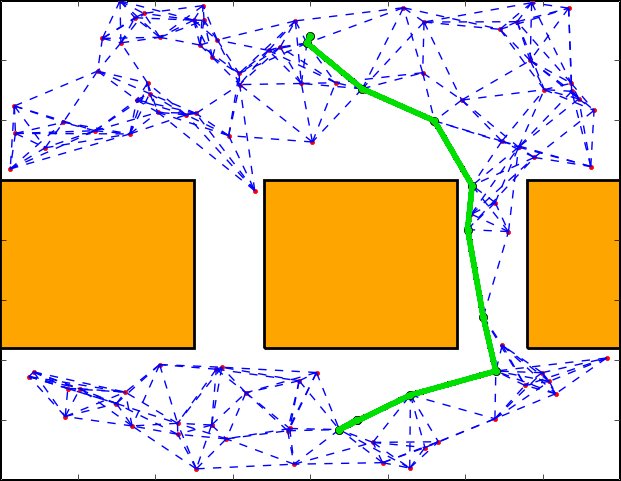
\includegraphics[width=.55\linewidth]{PRM} \quad
\caption[Example of a probabilistic roadmap (PRM) used to solve a start-to-goal
query.]
{Example of a probabilistic roadmap (PRM) used to solve a start-to-goal query.
The PRM was built with $100$ random samples, which were attempted to connect to
their $6$ nearest neighbors.}
\label{fig:PRM}
\end{figure}

\subsection{Single-query Methods}

There is another group of sampling-based algorithms that is devoted to solving a
single start-to-goal query. Such methods conduct an incremental search, which in
most cases is achieved by expanding a tree of randomly sampled configurations.
The search is generally biased to finding a solution path for one particular
start-to-goal query, rather than attempting to completely represent the
connectivity of $\mathcal{C}_{free}$. These methods are \textit{unidirectional}
when a single tree is expanded from $q_{start}$ until reaching $q_{goal}$ or
vice versa. Or, they are \textit{bidirectional} if two trees are expanded, one
from $q_{start}$ and other from $q_{goal}$, until both trees meet at a common
point. Choosing $q_{start}$ or $q_{goal}$ as the tree's root depends on the
specific problem and scenario, since there can be situations in which expanding
from the goal is easier (less constrained) that doing it from the start
configuration. There are different sampling-based single-query methods, however,
this section presents a brief review of those considered the most relevant.

\subsubsection{Randomized Path Planner (RPP)}

Section~\ref{sec:PotenFields} presented an approach for guiding a robot from its
current position towards the goal position, by following the negative gradient
of an artificial potential field. As mentioned there, one of the main
disadvantages of this approach is that the vehicle can get trapped in a local
minimum that may not correspond to the specified goal. In order to deal with
such situations, Barraquand and Latombe proposed in 1990 the randomized path
planner (\ac{RPP})~\cite{Barraquand1990,Barraquand1991}, which uses the strategy
of potential fields, but also incorporates random walks to escape local minima.
\ac{RPP} is commonly acknowledged as the first randomized algorithm. Albeit
\ac{RPP} has proved to be successful in many applications, it may fail when
coping with narrow passages.

\subsubsection{The Ariadne's Clew Algorithm (ACA)}

Presented in 1993, \ac{ACA} builds a tree from $q_{start}$ by interleaving the
\textit{exploration} of the \ac{C-Space} and the \textit{search} of a connection
between the tree and $q_{goal}$~\cite{Bessiere1993,Mazer1998}. During the
exploration, the algorithm places a random collision-free configuration as far
as possible from the others, therefore guaranteeing resolution completeness. New
configurations are selected by using genetic optimization methods. These
correspond to those from which a connection to $q_{goal}$ is attempted. The main
drawback of this approach is that the exploration of the \ac{C-Space} is
computationally expensive and also requires some parameter tuning.

\subsubsection{Expansive-Spaces Tree (EST)}

Proposed by David Hsu \etal in 1997,
\ac{EST}~\cite{Hsu1997,Hsu1999,Hsu2000,Hsu2002} is a single-query method that
incrementally builds a tree over the \ac{C-Space} by interleaving its
\textit{construction} and \textit{expansion}. In contrast to what occurs with
\ac{PRM} that computes a roadmap attempting to represent the whole
$\mathcal{C}_{free}$, \ac{EST} tries to sample the region of $\mathcal{C}$ that
is relevant in order to solve the specific start-to-goal query. To do so, during
the \textit{construction} phase the algorithm selects the node $q$ to be
extended in a way that prioritizes less explored regions, and then it randomly
samples a configuration $q_{rand}$ around $q$. Then, using a local planner,
\ac{EST} calculates the path that connects $q$ and $q_{rand}$. In case that both
$q_{rand}$ and the calculated path are proved collision-free, they will be added
to the tree, thus \textit{expanding} it.

\subsubsection{Rapidly-exploring Random Tree (RRT)}
\label{sec:RRT}

Within the group of sampling-based single-query algorithms, there is one method
that is considered the state-of-the-art, which has been extended, modified and
applied to a wide range of applications. This method is known as \ac{RRT} and
it was firstly presented by Steven LaValle in 1998~\cite{LaValle1998}.
\ac{RRT} is a tree-based algorithm that has different properties such as rapid
exploration of the \ac{C-Space}, probabilistic completeness, ease of
implementation, just to mention some. In 1999, LaValle and Kuffner formally
presented the \ac{RRT} as a path/motion planning method capable of dealing with
both geometric and motion constraints. They also proposed a greedy approach to
decrease the time required to find a solution by interleaving a random growing
of the tree with a biased growing towards the
goal~\cite{LaValle1999,LaValle2000,LaValle2001}. They later proposed a
bidirectional version called RRT-Connect that extends the basic concept by
constructing two \acp{RRT} towards each other~\cite{Kuffner2000}.

Similar to \ac{ACA} and \ac{EST}, the basic \ac{RRT} algorithm is mainly
composed of two main procedures, \textit{sample} and \textit{extend}.
Algorithm~\ref{alg:SampleRRT} presents the first of them, where the tree is
incrementally built until a stop condition occurs; such a condition can either
be finding a feasible path that reaches the goal close enough, or that a maximum
number of iterations has been completed. In each iteration, the \ac{RRT}
algorithm attempts to extend the tree towards a randomly sampled configuration
$q_{rand}$. For doing so, the second procedure described in
Algorithm~\ref{alg:ExtendRRT} finds $q_{near}$, which is the nearest
configuration to $q_{rand}$ in the tree (line~\ref{alg_line:findNearestGeom}).
Then, a local planner calculates a path of length $\delta$ from $q_{near}$
towards $q_{rand}$ (line~\ref{alg_line:ExtendRRTGeom}); if the path is proved
collision-free, the algorithm generates a new configuration $q_{new}$, which
together with the calculated path are added to the tree
(lines~\ref{alg_line:addNodeGeom}-\ref{alg_line:addEdgeGeom}). A typical growth
process of an \ac{RRT} algorithm can be clearly observed in
Figure~\ref{fig:RRT-Expansion}, where no goal has been specified and the tree
attempts to explore uniformly the \ac{C-Space}.
Figure~\ref{fig:RRT-Solve-Query} depicts the \ac{RRT} algorithm solving a
start-to-goal query.

\begin{algorithm}[htbp]
	\DontPrintSemicolon

	\SetKwFunction{stopCondition}{stopCondition}
	\SetKwFunction{initTree}{initTree}
	\SetKwFunction{generateRandomConf}{generateRandomConf}
	\SetKwFunction{extendRRT}{extendRRT}
	\SetKwFunction{addNode}{addNode}
	
	\KwIn{\\ 
	$q_{start}:$ Start configuration. \\ 
	$q_{goal}:$ Goal configuration.\\
	$\mathcal{C}$: \ac{C-Space}.}
	
 	\KwOut{\\ 
 	Rapidly-exploring Random Tree ($RRT$): T = $(V, E)$.}
 	
	\Begin{
		$V=\{ \, \}$\;
		$E=\{ \, \}$\;
		$V$.\addNode{$q_{start}$}\;
		\While{not \stopCondition{$T,goal$}}{
			$q_{rand}=\mathcal{C}.$\generateRandomConf{}\;
	 		\extendRRT{$T,q_{rand}$}\;
		}
	}
\caption{sampleRRT}
\label{alg:SampleRRT}
\end{algorithm}

\begin{algorithm}[htbp]
\DontPrintSemicolon

	\SetKwFunction{calcNewConf}{calcNewConf}
	\SetKwFunction{findNearestNeighbor}{findNearestNeighbor}
	\SetKwFunction{addNewNode}{addNewNode}
	\SetKwFunction{addNewEdge}{addNewEdge}
	
	\KwIn{\\ 
	$T$: an RRT.\\ 
	$q_{rand}$: configuration towards which RRT will be extended.\\
 	$\mathcal{C}$: \ac{C-Space}.}
	\KwOut{\\ Result after attempting to extend.}
	\Begin{
	 	$q_{near}\leftarrow T.$\findNearestNeighbor{$q_{rand}$}\;\label{alg_line:findNearestGeom}
	 	$q_{new}, collision\leftarrow$\calcNewConf{$q_{near},q_{rand},\delta$}\;\label{alg_line:ExtendRRTGeom}
	 	\If{$collision = FALSE$} { 
	 		V.\addNewNode{$q_{new}$}\;\label{alg_line:addNodeGeom}
	 		E.\addNewEdge{$q_{near},q_{new}$}\;\label{alg_line:addEdgeGeom}
	 		\KwRet{$\text{ADVANCED}$}\label{lin_alg:Adva}
  		}
  		\Else{
  			\KwRet{$\text{TRAPPED}$}\label{lin_alg:Trapp}
  		}
 	}
\caption{extendRRT}
\label{alg:ExtendRRT}
\end{algorithm}

\begin{figure}[htbp]
    \myfloatalign
    \subfloat[RRT expansion]
    {\label{fig:RRT-Expansion}
    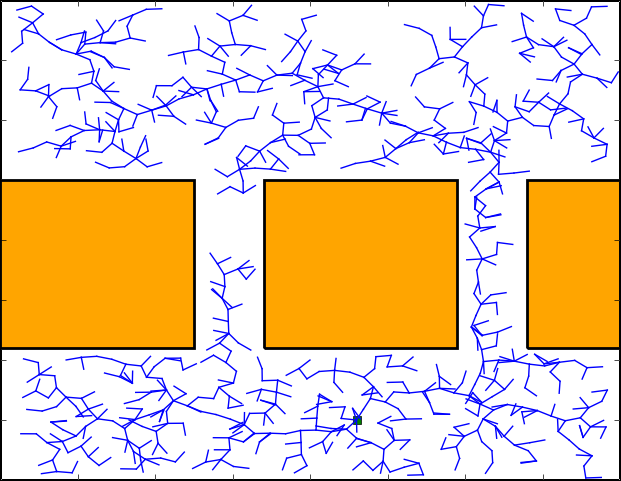
\includegraphics[width=.45\linewidth]{RRT-Expansion}} \quad
    \subfloat[RRT solving a query]
    {\label{fig:RRT-Solve-Query}%
     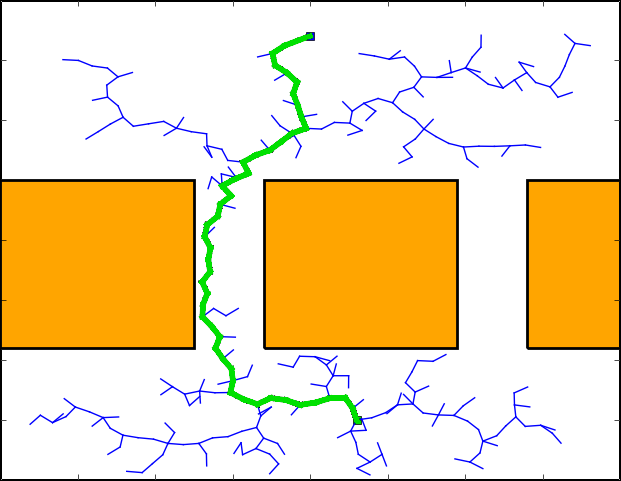
\includegraphics[width=.45\linewidth]{RRT-Solve-Query}}
\caption[Example of a rapidly-exploring random tree (RRT).]
{Example of a rapidly-exploring random tree (RRT) in a 2D workspace. 
\protect \subref{fig:RRT-Expansion} The uniform and rapid exploration of the
C-Space is one of the main characteristics.
\protect \subref{fig:RRT-Solve-Query} The expansion of the tree stops once a
solution has been found.}
\label{fig:RRT}
\end{figure}

\subsection{Optimal Planning}
\label{sec:SamplOptimalPlan}

At least in their original formulation, sampling-based algorithms do not
guarantee that the calculated path is optimal with respect to a specified cost
function. However, more recent contributions have attempted to cope with this
situation. In 2010, Jaillet \etal presented the \ac{T-RRT}, which calculates a
low-cost path that follows valleys and saddle points in a costmap established
over the \ac{C-Space}~\cite{Jaillet2010}. To achieve this, it verifies the
quality of the path by using the minimal work criterion. Its key principle is
that positive variations of the cost function can be seen as forces acting
against motion, and thus producing mechanical work. Contrasted to a standard
\ac{RRT} algorithm implementation, an additional transition validation is
performed, which accepts or rejects new potential configurations before adding
them into the solution tree.

Nonetheless, the state-of-the-art sampling-based method for calculating optimal
paths is the \ac{RRT*}. In 2010, Karaman and Frazzoli firstly introduced the
\ac{RRT*} algorithm and its concept of asymptotic optimality. This property
states that the total cost of the solution, measured by a user-defined function,
decreases as the number of samples increases~\cite{Karaman2010a}. In this
approach, new configurations are connected to the closest and best
configuration, \ie the one that guarantees a minimum cost. Furthermore, an
additional step of sample reconnection allows improving costs to surrounding
configurations (see Algorithm~\ref{alg:ExtendRRTstar}). This concept was later
extended by the same authors to the \ac{PRM} in~\cite{Karaman2011}, where they
formally presented the \ac{RRT*} and PRM* algorithms. Similar extensions have
been done to other RRT-based algorithms as \ac{T-RRT} and its respective T-RRT*
version~\cite{Devaurs2016}. A typical growth process of an \ac{RRT*} algorithm
can be clearly observed in Fig.~\ref{fig:RRTstar}.

\begin{algorithm}[htbp]
    \DontPrintSemicolon

	\SetKwFunction{buildRRT}{buildRRT}
	\SetKwFunction{calculatePath}{calculatePath}
	\SetKwFunction{findNearestNeighbor}{findNearestNeighbor}
	\SetKwFunction{addNewNode}{addNewNode}
	\SetKwFunction{addNewEdge}{addNewEdge}
	\SetKwFunction{findNearestNeighbors}{findNearestNeighbors}
	\SetKwFunction{findMinCost}{findMinCost}
	\SetKwFunction{reconnectNearNeighbors}{reconnectNearNeighbors}
	\SetKwFunction{findInput}{findInput}
	
	\KwIn{\\
	$T$: tree of collision-free configurations.\\
	$q_{rand}$: state towards which the tree will be extended.\\
 	$\mathcal{C}$: C-Space.}
	\KwOut{\\ 
	Result after attempting to extend.}
	\Begin{
	 	$q_{near}\leftarrow T.$\findNearestNeighbor{$q_{rand}$}\;
	 	$q_{new}, collision\leftarrow$\calcNewConf{$q_{near},q_{rand},\delta$}\;%label{alg_line:ExtendRRTGeom}
	 	\If{$collision = FALSE$} {
  			\addNewNode{$T,q_{new}$}\;
  			$Q_{near}\leftarrow$\findNearestNeighbors{$T,q_{new}$}\;\label{lin_alg:FindNearNeighbors}
  			$q_{min\_cost}\leftarrow$\findMinCost{$T,Q_{near},q_{new}$}\;\label{lin_alg:FindMinCost}
  			\addNewEdge{$T,q_{min\_cost},q_{new}$}\;\label{lin_alg:AddNewEdge}
  			\reconnectNearNeighbors{$T,Q_{near},q_{new}$}\;\label{lin_alg:ReconnNearNeighbors}
  			\KwRet{$\text{ADVANCED}$}\;%\label{lin_alg:Adva}
  		}
  		\Else{
  			\KwRet{$\text{TRAPPED}$}\;%\label{lin_alg:Trapp}
  		}
 	}
\caption[extendRRT*]{extendRRT*}
\label{alg:ExtendRRTstar}
\end{algorithm}


\begin{figure}[htbp]
    \myfloatalign
    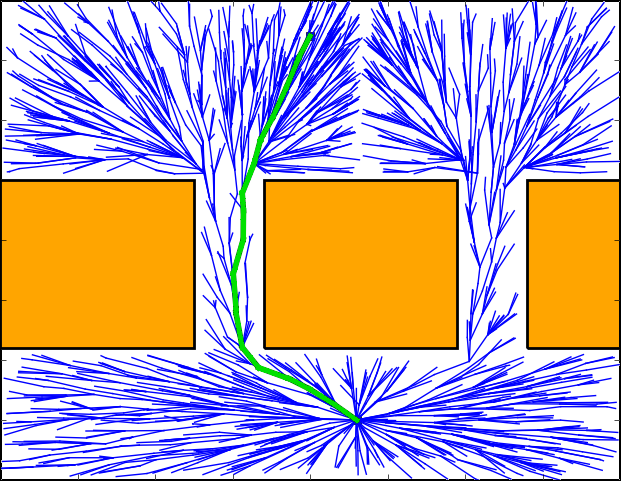
\includegraphics[width=.55\linewidth]{RRTStar-Expansion}
\caption[Example of an asymptotic optimal rapidly-exploring random tree (RRT*).]
{Example of an asymptotic optimal rapidly-exploring random tree (RRT*) in a 2D
workspace. The RRT* preserves the uniform and rapid exploration of the C-Space
as the standard RRT; however, it can be observed how the additional reconnection
step reshapes the tree branches. The expansion of the tree does not stop once a
solution has been found. Instead, it keeps improving the solution until either a
maximum number of iterations or a maximum time has been reached.}
\label{fig:RRTstar}
\end{figure}

% \begin{algorithm}[htbp]
% 	\dontprintsemicolon
% 	\SetKwFunction{findNearestNeighbor}{findNearestNeighbor}
% 	\SetKwFunction{findInput}{findInput}
% 	\SetKwFunction{calcNewConf}{calcNewConf}
% 	\SetKwFunction{addNewNode}{addNewNode}
% 	\SetKwFunction{addNewEdge}{addNewEdge}
% 	\SetKwFunction{findNearestNeighbors}{findNearestNeighbors}
% 	\SetKwFunction{findMinCost}{findMinCost}
% 	\SetKwFunction{reconnectNearNeighbors}{reconnectNearNeighbors}
% 	
%  	\KwIn{\\ $T$: configurations tree (RRT).\\
%  			  $q_{rand}$: state which RRT will be attempted to extend to.\\}
%  	\KwOut{\\ Result after attempting extension. \\
%  			  $q_{new}$: New configuration if succeeded.}
%  	
%  	\Begin{
%   		$q_{near}\leftarrow$\findNearestNeighbor{$T,q_{rand}$}\;
%   		$u_{near\_rand}\leftarrow$\findInput{$T,q_{near},q_{rand}$}\;\label{lin_alg:FindInputRRT}
%   		$q_{new}, collision\leftarrow$\calcNewConf{$q_{near},u_{near\_rand}$}\;
%   		\If{{\bf not} $collision$} { 
%   			\addNewNode{$T,q_{new}$}\;
%   			$Q_{near}\leftarrow$\findNearestNeighbors{$T,q_{new}$}\;\label{lin_alg:FindNearNeighbors}
%   			$q_{min\_cost}\leftarrow$\findMinCost{$T,Q_{near},q_{new}$}\;\label{lin_alg:FindMinCost}
%   			\addNewEdge{$T,q_{min\_cost},q_{new}$}\;\label{lin_alg:AddNewEdge}
%   			\reconnectNearNeighbors{$T,Q_{near},q_{new}$}\;\label{lin_alg:ReconnNearNeighbors}
%   			\KwRet{$\text{ADVANCED}$}\label{lin_alg:Adva}
%   		}
%   		\Else{
%   			\KwRet{$\text{TRAPPED}$}\label{lin_alg:Trapp}
%   		}
%  }
%  \caption{extendRRT$(T,q_{rand})$}
%  \label{alg:ExtendRRT}
% \end{algorithm}

% \cite{Ferguson2006}
% \cite{Li2002}
% 
% \cite{Bruce2002}, \cite{Stentz1995}, \cite{Carsten2006}, \cite{Leven2002},
% \cite{Barraquand1990}, \cite{Shvalb2013}, \cite{Valencia2012}, \cite{Mora2013},
% \cite{Karaman2011}, \cite{Salzman2013}, \cite{Muller2011}, \cite{Zhu2013},
% \cite{Poppinga2011}, \cite{Li2010}, \cite{Ardiyanto2011}, \cite{Dobson2013},
% \cite{Sucan2008}, \cite{Howard2014}, \cite{Ladd2005}, \cite{Ghosh2008},
% \cite{Xue2009}, \cite{Dolgov2010}, \cite{Smith2010}, \cite{Likhachev2009},
% \cite{Dolgov2008}, \cite{Aoude2013}, \cite{Maki2007}, \cite{Vannoy2008},
% \cite{Quinlan1994}, \cite{Kuwata2009}, \cite{Karaman2011}, \cite{Tsianos2007},
% \cite{Masehian2008}, \cite{Dobson2012,Dobson2014}, \cite{Thrun2006},
% \cite{Kewlani2009}, \cite{Kim2009}
% 
%  
% 
% However, one of them, a graph-based approach known as
% \textit{\ac{RRG}}~\cite{Karaman2009}, attempts to minimize a cost function.
% That method has been modified in order to guarantee an asymptotic optimality as
% is known as
% \textit{\ac{RRT*}}~\cite{Karaman2010,Karaman2010,Karaman2011,Karaman2011}

% ----------------------- another section  ------------------------
\section{Extensions and Applications}
\label{sec:ExtensionsApplications}

Most of the aforementioned methods have been widely used in real-world
applications not only with manipulator arms, but also with different aerial,
terrestrial and aquatic robotic systems. For doing so, some of these methods
have been extended and adapted according to the specific applications'
requirements. Considering the problem and objectives stated for this thesis in
Chapter~\ref{ch:introduction}, this section presents a brief review of the most
relevant extensions and applications of path/motion planning algorithms, which
have permitted conducting autonomous missions under both motion and online
computation constraints.

% ----------------------- subsection  ------------------------
\subsection{Planning Feasible Paths}
\label{sec:motion_constraints_review}

As explained in Section~\ref{sec:PlannUnderConst}, planning under motion
(differential) constraints has to do with considering the limits of the feasible
system's maneuvers. These are described by a set of differential equations,
generally expressed as $\dot{q}=f\left(q,u\right)$ (where $q$ and $\dot{q}$ are
the system state and its first derivative, respectively, and $u$ is the control
input). A large body of research has been dedicated to the development and
improvement of different approaches attempting to solve planning problems that
include this kind of constraints.

When Donald \etal formally introduced the problem of kinodynamic motion
planning\footnote{Kinodynamic motion planning alternatively refers to motion
planning under motion or differential constraints.}, they proposed the use of
dynamic programming to find the shortest path in a directed graph using
\ac{DFS}. In this case, the graph represents a discretization of
$\mathcal{C}_{free}$; the edges correspond to trajectory segments obtained after
applying an acceleration $a$ (bounded according to the system's capabilities)
for a period of time $\tau$ (determined by the algorithm)~\cite{Donald1993}.

Other variants of grid-based methods, such as A*, have been also used with
similar strategies for discretizing $\mathcal{C}_{free}$. In terrestrial
vehicles, for example, the most remarkable contributions were a result of the
DARPA Grand Challenge~\cite{Thrun2006}\footnote{The DARPA Grand Challenge is a
competition of autonomous vehicles, funded by the Defense Advanced Research
Projects Agency (DARPA).}. In one of those works, Likhachev and Ferguson used a
multi-resolution lattice state space (a $\mathcal{C}_{free}$ discretization),
where states represent configurations, and connections between them represent
feasible paths (\ie those that consider kinematic constraints).
Then, one A* variant (called AD*) would find paths over the
lattice~\cite{Likhachev2009}. Similarly, Dolgov \etal presented an approach in
which $\mathcal{C}_{free}$ is also discretized and paths are found by running
another A* variant (Hybrid-State A*). This is guided by two heuristics, one that
considers the vehicle's non-holonomic constraints and a second one that computes
the Euclidean distance. This approach also connects the states (configurations)
by restricting the control inputs according to the feasible (doable) maneuvers
of a car-like system, which are expressed by non-holonomic (kinematic)
constraints~\cite{Dolgov2008,Dolgov2010}.

% In all these grid-based approaches, the main drawback is given by the
% $\mathcal{C}_{free}$ discretization, which establishes a finite set of possible
% maneuvers, thus limiting the number of possible solution paths. As occurs with
% geometric path planning approaches, the availability of a solution depends on
% the grid resolution and, in this case, on the number of maneuvers considered
% according to the motion constraints.

In what concerns sampling-based methods, \ac{EST} and \ac{RRT} algorithms were
initially conceived to cope with motion constraints~\cite{Hsu2002,LaValle2001}.
In their original versions, the differential equation of motion is used to
generate new nodes (states) during the \textit{expansion} of the tree (\eg in
Algorithm~\ref{alg:ExtendRRT}, line 3)\footnote{While tree and graph nodes are
generally referred to as configurations in geometric path planning, in
kinodynamic motion planning they are commonly called states. However, this
latter term has been indistinctly used by some authors to refer to them in
either case.}. Figure~\ref{fig:PlannConst} depicts two sampling-based
algorithms: \ac{RRT*} and \ac{RRT} in the process of solving a start-to-goal
query in a \ac{2D} workspace under both geometric and motion constraints.

\begin{figure}[htbp] \myfloatalign
	\subfloat[Geometric Constraints] {\label{fig:PlannGeomConstr_}
    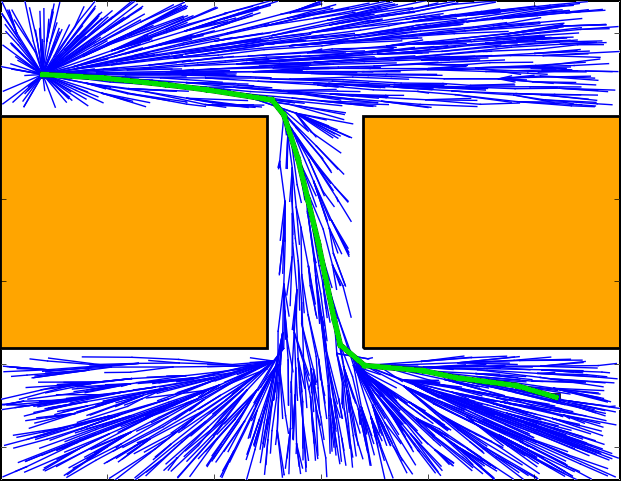
\includegraphics[width=.4\linewidth]{PlannGeomConstr}} \quad
    \subfloat[Differential Constraints] {\label{fig:PlannDiffConstr}
    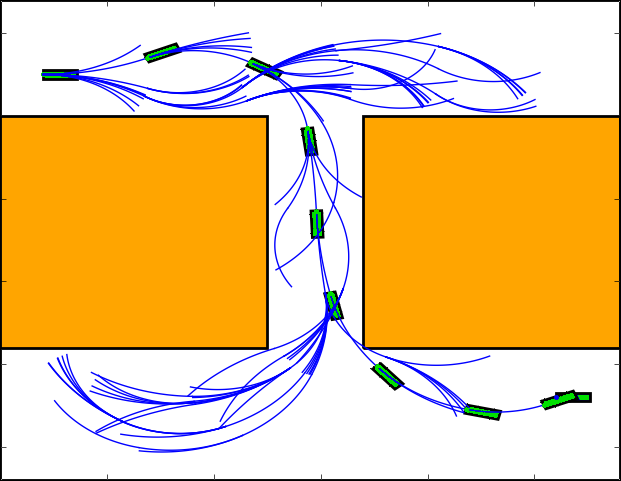
\includegraphics[width=.4\linewidth]{PlannDiffConstr}}
\caption[Comparison between start-to-goal query solutions under geometric and
differential constraints over a 2D workspace.]
{Start-to-goal query solution in a \ac{2D} workspace, where obstacles appear in
orange, free space in white, and the tree of collision-free configurations in
blue. The solution (in green) is calculated by
\protect \subref{fig:PlannGeomConstr_} an \ac{RRT*} algorithm under geometric
constraints for a point-like system $\left(\mathcal{C} = \mathbb{R}^{2}\right)$,
and
\protect \subref{fig:PlannDiffConstr} an \ac{RRT} algorithm under differential
constraints for a car-like system $\left(\mathcal{C} = \mathbb{R}^2 \times
\mathcal{S} \right)$.}
\label{fig:PlannConst}
\end{figure}

There are several successful applications based on this approach. In terrestrial
vehicles, one of the most relevant application was presented by Kuwata \etal
during The DARPA Urban Challenge. They proposed an approach known as
\ac{CL-RRT}, which not only considers the vehicle's motion model, but also
includes the controller's dynamic behavior~\cite{Kuwata2009}. Another
interesting application was done with aerial systems, in which M\"uller \etal
proposed to use an A* for globally finding the collision-free path which, at the
same time, guides an \ac{RRT} algorithm expanded under differential constraints.
This latter guarantees finding paths that meet the system's motion
constraints~\cite{Muller2011}.

% ----------------------- subsection  ------------------------
\subsection{Online Path/Motion Planning}

As discussed in Chapter~\ref{ch:introduction}, potential and new applications
for \acp{AUV} involve navigating unknown or undiscovered environments that
require endowing the vehicles with the capability of (re)planning online while,
at the same time, they explore the environment. There are different extensions
that can contribute to achieving this requirement, however this section focuses
on two of them. The first is the \textit{anytime} computation, a characteristic
incorporated to different kind of algorithms, including both search-based and
sampling-based methods. The second refers to \textit{lazy collision checking}, a
strategy specifically used with sampling-based methods. These two
characteristics have served as a basis for the proposed approach of this thesis.

% ----------------------- subsubsection  ------------------------
\subsubsection{Anytime Planning Algorithms}

In some situations finding a definite path to solve a start-to-goal query in a
finite and deterministic period of time is not possible. It may occur either
because of the complexity of the task (\ie more computation time is required) or
because vehicles deal with partially known or dynamic environments. In either
case, a common approach is to use an \textit{anytime} algorithm that is capable
of providing the best partial solution when the available time is
over~\cite{Zilberstein1995},\cite{Dean1988}. The most relevant and well-known
planning algorithms have been extended based on this strategy.

Likhachev \etal have studied search-based algorithms, including their extensions
for \textit{anytime} computation. They presented the \ac{ARA*}, a variant that
rapidly calculates a suboptimal path to the goal using a loose bound, which is
later tightened to progressively improve the path~\cite{Likhachev2003}. While
this approach obtains a fast solution, it also permits improving it if
additional time is available. Nonetheless, this approach is useful when
full and accurate information about the environment is available, otherwise it
may require recalculating the whole path if the environment changes. For those
cases, \ie when coping with dynamic environments, it is better to use an
incremental search-based method as \ac{D*}, which allows locally repairing
(replanning) the path when new information of the environment is provided (see
Section~\ref{sec:D-star}). However, in its original version, \ac{D*} lacks the
\textit{anytime} property. In order to improve \ac{D*}'s characteristics,
Likhachev \etal also presented the \ac{AD*}. This is a variant that not only
replans if required, but also improves simultaneously the available solution
path~\cite{Likhachev2005}. A detailed discussion of these \textit{anytime}
search-based algorithms is provided in~\cite{Likhachev2008}.
Some applications for vehicles that not only require online/anytime computation,
but also navigate under motion constraints are also presented
in~\cite{Likhachev2009}.

In the case of sampling-based methods there are also different extensions for
\textit{anytime} computation. Belghith et. al, for example, proposed the
\ac{FADPRM}, which is an approach that combines both: a standard \ac{PRM} for
constructing the roadmap and an \ac{AD*} for finding a solution path. This
latter one extends the original \ac{PRM} by permitting not only \textit{anytime}
calculation, but also a progressive improvement of the resulting path. An
important characteristic of this approach is the possibility to establish zones
with different values of desirability that allow the sampling strategy to be
influenced in order to generate less awkward (inefficient and not smooth)
paths~\cite{Belghith2006}. A similar approach presented by van den Berg
\etal uses \ac{PRM} to represent the static portion of \ac{C-Space} and an
\ac{AD*} to deal with the dynamic elements~\cite{VandenBerg2006}.

On the other hand, and because of its incremental nature, randomized tree-based
methods, such as \ac{RRT} algorithm, are more commonly used for applications in
partly known or dynamic environments, where online and \textit{anytime}
computation is required. Ferguson \etal proposed an anytime RRT-based algorithm
that calculates an initial path and its cost using the standard \ac{RRT}, thus
ensuring that a first solution is found in the shortest time possible. Then, a
modified \ac{RRT} algorithm iteratively generates a series of new solutions that
are guaranteed to have a lower cost. The algorithm executes until a stop
condition is reached, \eg when the best available solution path needs to be
provided~\cite{Ferguson2006,Ferguson2007}. Other RRT variants as \ac{RRT*} were
also formulated as \textit{anytime} algorithms~\cite{Karaman2011a}.

% Online:
% \cite{Stentz1995}, \cite{Bruce2002}, \cite{Koenig2002}, \cite{Jaillet2004},
% \cite{Maki2009}, \cite{Dolgov2008}, \cite{Kewlani2009}, \cite{Kuwata2009},
% \cite{Likhachev2009}, \cite{Dolgov2010}, \cite{Ardiyanto2011},
% \cite{Muller2011}, \cite{Aoude2013}, \cite{Fulgenzi2009}
% Petti and Fraichard~\cite{Petti2005} presented a tree-based \ac{PMP}, which
% uses limited time slots to obtain updated models of the environment with
% predictions of moving obstacles in order to recalculate the best partial plan.
% First extensions of basic algorithms to support online replanning
% D*~\cite{Stentz1995}, \cite{Koenig2002}, PRM~\cite{Leven2002,Jaillet2004}
% 
% \cite{Likhachev2003}, \cite{Likhachev2005}, \cite{Belghith2006},
% \cite{Karaman2011}, \cite{VandenBerg2006}, \cite{Ferguson2006},
% \cite{Ferguson2007}, \cite{Salzman2013}, \cite{Perez2011},
% \cite{Guibas2009}, \cite{Hornung2013}, \cite{Karaman2010},
% \cite{Likhachev2009}, \cite{Fulgenzi2009}, \cite{Aoude2013},
% \cite{Vannoy2008}, \cite{Karaman2011}, \cite{Jaillet2010},
% \cite{Elbanhawi2014}, \cite{Kurniawati2008}, \cite{Hatton2013}

% ----------------------- subsubsection  ------------------------
\subsubsection{Lazy Collision Checking}
\label{sec:lazy_collision_check}

Even though \ac{PRM} was originally intended for multi-query applications,
Bohlin and Kavraki presented a modified version known as Lazy PRM, which
minimizes the execution time by reducing the quantity of collision checking
callbacks when solving a specific (single) query~\cite{Bohlin2000,Bohlin2001}.
This variant builds a roadmap just as a standard \ac{PRM} does, but it assumes
that all the nodes (configurations) and edges (paths between configurations) are
collision-free, leaving the collision detection to the final stage, \ie when it
must find the shortest path between an initial and a final configuration. If a
collision is found, the associated nodes and edges are discarded (eliminated)
and a new short path is calculated. The authors also suggested an optional
\textit{enhancing roadmap} step when collisions are indeed detected. This
consists in including more samples around the discarded nodes.

This strategy of delaying the collision detection is known as \textit{lazy
collision checking}, and has been used in different applications, especially
those with online computation requirements. Bekris and Kavraki, for instance,
proposed and validated a tree-based planning framework for terrestrial vehicles,
where the states validity is only checked once a path between the start and the
goal configuration has been found~\cite{Bekris2007}. Another example is the one
presented by Vahrenkamp et al., where this strategy was used to speed up the
motions calculation for humanoid robots (with many degrees of freedom, \ie high
dimensional \ac{C-Space})~\cite{Vahrenkamp2007}.

Finally, it is important to note that \textit{lazy collision checking} has
served as a base for one of the extensions proposed and used in this thesis,
which will be explained in detail in Chapter~\ref{ch:plann_online}.

% ----------------------- another section  ------------------------
\section{Path/Motion Planning for AUVs}
\label{sec:StateOfTheArtPlannAUV}

An important aspect to consider when comparing the path/motion planning
approaches for \acp{AUV} is their application. Based on this, the different
contributions can be classified into two main categories. The first group
gathers those applications that require \acf{CPP} techniques, which are commonly
applied to guide \acp{AUV} over survey tasks. The most common examples within
this group include coverage missions used for creating detailed bathymetric
maps of the seabed~\cite{Fang2010, Galceran2012, Galceran2013b, Galceran2013d},
detecting potential targets (such as underwater mines~\cite{Stack2003,
Williams2010}), and inspecting artificial structures (such as in-water ship
hulls~\cite{Englot2010, Hover2012, Hollinger2013, Englot2013}), as well as
natural marine formations~\cite{Galceran2014,Galceran2014b}.

A common characteristic in all these approaches is that the planner is provided
with preliminary information of the target area or structure (see
Fig.~\ref{fig:CPP-App}). This may include its location and shape. Based on this,
the \ac{CPP} algorithm defines a survey path that, in some cases, is reshaped or
refined online according to the data obtained during the mission execution. This
characteristic implies that most of the computation is done offline, \ie before
conducting the mission. Most recent work presented by Vidal \etal proposes a
novel approach to conduct inspection tasks without preliminary information of
the target. Results are, however, still limited to \ac{2D} motions (at a
constant depth)~\cite{Vidal2017}.

\begin{figure}[htbp]
    \myfloatalign
    \subfloat[Coverage path over of a natural formation. Image credit: Galceran
    \etal\cite{Galceran2013b}]
    {\label{fig:CPP-NaturalFormation}
    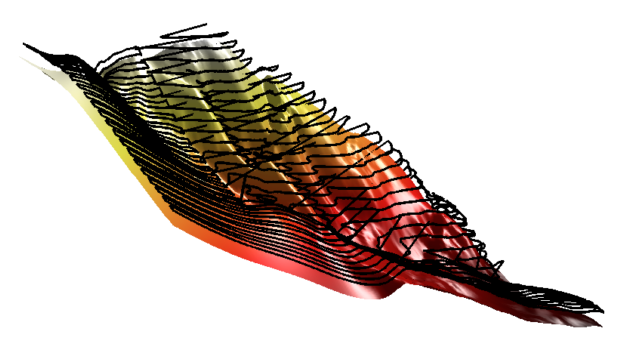
\includegraphics[width=.5\linewidth]{CPP-NaturalFormation}} \\
    \subfloat[Coverage path of a ship hull. Image credit: Hover
    \etal\cite{Hover2012,Englot2013}] 
    {\label{fig:CPP-ShipHull}%
     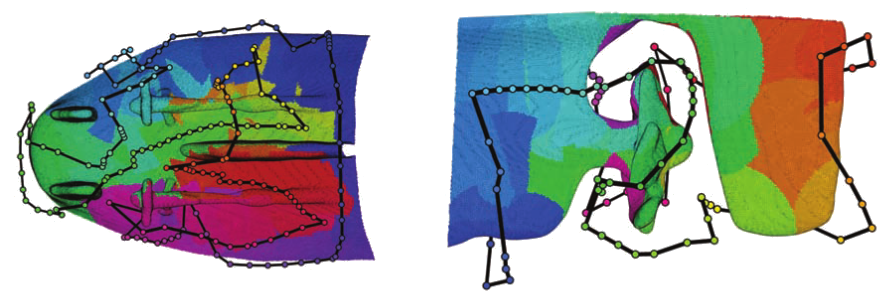
\includegraphics[width=.90\linewidth]{CPP-ShipHull}}
\caption[Coverage path planning (CPP) applications.]
{Coverage path planning (CPP) algorithms are normally used to plan routes to
inspect different kind of structures. In most of these applications the planner
has preliminary information. This may include a 2D/3D map of the area or
structure to be inspected.}
\label{fig:CPP-App}
\end{figure}

The second group of \ac{AUV} applications, on the other hand, gathers those that
are focused on safely and efficiently guiding the vehicle from one initial
position to a specified goal. For doing so, different strategies, such as those
explained throughout previous sections, have been applied to underwater
vehicles. In fact, these start-to-goal methods are commonly used as low-level
motion planners required for the aforementioned coverage applications. The work
presented throughout this thesis seeks to make contributions to this group of
start-to-goal applications, therefore it is important to identify the main
characteristics between the different approaches used.

\subsection{Start-to-goal Path/Motion Planning for AUVs}

One characteristic to consider in a start-to-goal planner for \acp{AUV}, and yet
not an obvious one, is the capability of conducting \ac{2D} and \ac{3D} motions.
Although \acp{AUV} operate in \ac{3D} workspaces, in a significant number of
applications the vehicles navigate either at a constant altitude or at a
constant depth~\cite{Petillot2001,Poppinga2011,Soulignac2011,McMahon2016}, thus
simplifying considerably the motion planning problem. There are, however, some
contributions that have presented alternatives in modelling and planning \ac{3D}
(and therefore \ac{2D}) \ac{AUV} motions.

From the approaches that address \ac{3D} motions, the available contributions
have made use of different approaches such as potential
fields~\cite{Warren1990,Sequeira1994}, genetic
algorithms~\cite{Sugihara1997,Alvarez2004,Hong-jian2004}, as well as
sensor-based~\cite{Ying2000,Houts2012},
grid-based~\cite{Carroll1992,Sequeira1994,Kim2012a}, and sampling-based
methods~\cite{Caldwell2010,Poppinga2011,McMahon2016}. However, in some of these
situations, the vehicle operates in open sea areas, where they do not usually
have to deal with obstacles, narrow passages, or high-relief environments. This
kind of constraints corresponds to the new and potential \ac{AUV} applications
presented in Chapter~\ref{ch:introduction}.
% In such situations, the planner must be capable of safely guiding the \ac{AUV}
% through unexplored environments, which requires to meet online computation
% limitations while considering the vehicle's motion capabilities.

%\begin{figure}[htbp]
%    \myfloatalign
%    \subfloat[Glider sinusoidal-like vertical motion. Image credit: Thompson
%    \etal\cite{Thompson2010}]
%    {\label{fig:GlidersMissions3D}
%    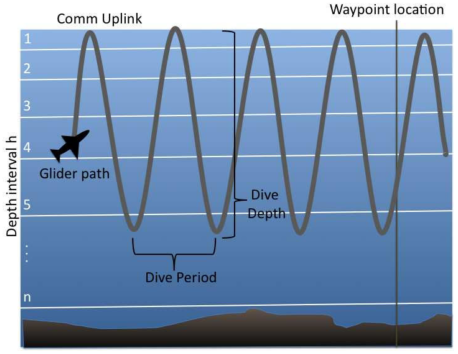
\includegraphics[width=.48\linewidth]{GlidersMissions3D}} \quad
%    \subfloat[Glider one-month-long mission. Image credit: Smith
%    \etal\cite{Smith2010}] 
%    {\label{fig:GlidersMissionsTop}%
%     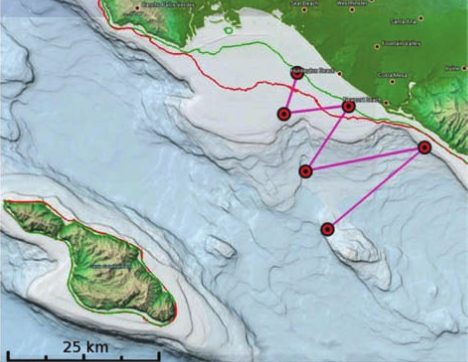
\includegraphics[width=.48\linewidth]{GlidersMissionsTop}}
%\caption[Examples of underwater gliders missions.]
%{\protect \subref{fig:GlidersMissions3D} Due to their propulsion mechanisms,
%underwater gliders normally follow sinusoidal-like trajectories.
%\protect \subref{fig:GlidersMissionsTop} They conduct long-term missions
%and operate in open sea and obstacle-free areas.}
%\label{fig:GlidersMissions}
%\end{figure}

\subsection{Online Motion Planning for AUVs through Unexplored Environments}

New \ac{AUV} applications require a path/motion planner to safely guide the
vehicle through unexplored and challenging environments. This implies meeting
online computation limitations while, at the same time, considering the
vehicle's motion capabilities. Little research on this area, especially for
underwater vehicles, has been addressed. In what concerns to generating \ac{AUV}
feasible paths, \ie those that meet the motion constraints, a first group
includes those approaches that use sensor-based methods either to navigate
through unknown underwater environments~\cite{Ying2000}, or to follow the
terrain shape of a given bathymetric map~\cite{Houts2012} (see
Fig.~\ref{fig:SensorBasedConstrainedAUV}). In both cases, the vehicle is assumed
to be equipped with a forward-looking sonar to reactively avoid collisions. Such
maneuvers are calculated by a local planner that meets the \ac{AUV}'s kinematics
or dynamics. An important characteristic of this kind of approach is the lack of
global knowledge of the environment (\ie a map is not incrementally built),
which can cause the vehicle to get trapped in complex scenarios.

\begin{figure}[htbp]
    \myfloatalign
    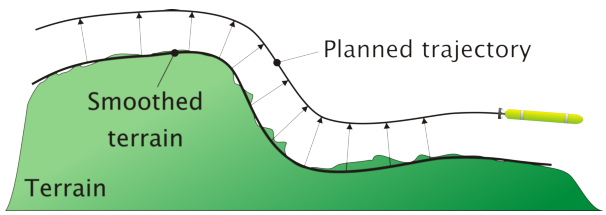
\includegraphics[width=.85\linewidth]{SensorBasedConstrainedAUV}
\caption[Sensor-based planning for AUVs under motion constraints.]
{Sensor-based planning for AUVs under motion constraints. The vehicle trajectory
can be either preplanned or incrementally calculated to maintain a desired
distance from the terrain. The resulting trajectory is fit to satisfy
curvature constraints that approximate the AUV motion constraints. Image credit:
Houts \etal\cite{Houts2012,Houts2014}.}
\label{fig:SensorBasedConstrainedAUV}
\end{figure}

A similar reactive approach establishes a set of inequality constraints that
describes the obstacles as convex regions contained in the
\ac{C-Space}~\cite{Petillot2001}. The initial configuration is treated
as the starting point of a nonlinear search, where the goal configuration is
assumed to be a unique global minimum of the objective function. The
start-to-goal query is then solved as an optimization problem, in which a local
planner takes into account the vehicles' constraints. This strategy was one of
the first online obstacle avoidance approaches for underwater vehicles; it used
a real-world dataset of acoustic images obtained by a \ac{ROV} equipped with a
multibeam forward-looking sonar. Its validity was demonstrated by guiding a
simulated \ac{ROV}. However, the capability of simultaneous mapping (detection)
and planning online was not established.

A formulation that represents obstacles as convex regions has likewise been
used either to represent obstacles detected online, which triggers collision
avoidance maneuvers~\cite{Qu2009}, or to approximate the terrain shape that must
be followed by the vehicle~\cite{Murthy2010}. In both cases, the low-level
controller attempts to generate feasible trajectories by using the
\ac{AUV} kinematic equations and spline-based interpolation techniques,
respectively. However, the main drawback of these approaches is the difficulty
in creating a convex representation of complex obstacles.

Another common strategy used in some of the aforementioned methods, is trying to
get as close as possible to a path that can be followed by an \ac{AUV}. Pêtrès
et al., for instance, proposed a \ac{FM}-based approach to find collision-free
paths, which are smoothed by a cost function that contains kinematic and
curvature constraints~\cite{Petres2007} (see
Fig.~\ref{fig:CostFunctionConstrainedAUV}). Likewise, another example based on
\acp{GA} finds a valid route to the goal by using \ac{B-spline} curves, thus
seeking to generate more feasible trajectories for \acp{AUV}~\cite{Cheng2010}.

\begin{figure}[htbp]
    \myfloatalign
    \subfloat[]
    {\label{fig:CostFunctionConstrainedAUV-a}
    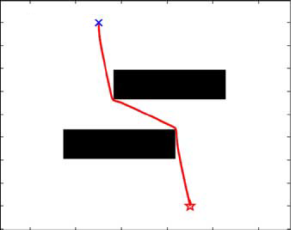
\includegraphics[width=.3\linewidth]{CostFunctionConstrainedAUV-a}} \quad
    \subfloat[] 
    {\label{fig:CostFunctionConstrainedAUV-b}%
     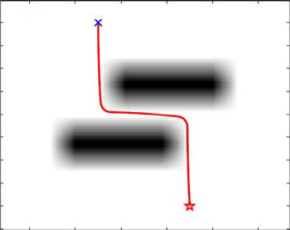
\includegraphics[width=.3\linewidth]{CostFunctionConstrainedAUV-b}} \quad
     \subfloat[] 
    {\label{fig:CostFunctionConstrainedAUV-c}%
     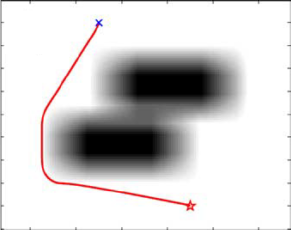
\includegraphics[width=.3\linewidth]{CostFunctionConstrainedAUV-c}}
\caption[FM-based planning for AUVs under motion constraints.]
{Start-to-goal query that is solved by a FM-based method. The solution path is
smoothed by a cost function to approximate the AUV motion constraints.
\protect \subref{fig:CostFunctionConstrainedAUV-a} The initial optimal path.
\protect \subref{fig:CostFunctionConstrainedAUV-b} The effect after smoothing the
path.
\protect \subref{fig:CostFunctionConstrainedAUV-c} The use of the cost function
can merge the obstacles, thus discarding possible solutions. Image credit:
Pêtrès \etal\cite{Petres2007}.}
\label{fig:CostFunctionConstrainedAUV}
\end{figure}

Unlike the previous group of sensor-based approaches, the second group of path
planning methods for motion-constrained \acp{AUV} uses grid-based approaches.
Sequeira and Ribeiro, for example, presented a two-layer framework that is
composed of a \ac{HLP} and a \ac{LLP}~\cite{Sequeira1994}. The \ac{HLP} creates
a visibility graph using the information of the known obstacles, sea currents,
and specified waypoints of the mission. Furthermore, the energy required to move
between the graph nodes corresponds to the edge weights. The global and optimal
geometric route to the goal is then found by Dijkstra's algorithm. Finally, in
order to calculate the vehicle's maneuvers between the different solution
segments, the \ac{LLP} uses an \ac{AFP}. This way the total artificial force
includes a \ac{3D} double integrator that takes into account the \ac{AUV} motion
constraints. There are other similar two-layer approaches, where the global path
planning problem is tackled with a grid-based method, and the local motion
planning deals with the \ac{AUV} constraints~\cite{Arinaga1996} (see
Fig.~\ref{fig:GridBasedLocalConstrAUV}). The main disadvantage of line of works
is that the grid-based layer generally requires \textit{a priori} information of
the environment, \eg a navigation map.

\begin{figure}[htbp]
    \myfloatalign
    \subfloat[]
    {\label{fig:GridBasedLocalConstrAUV-a}
    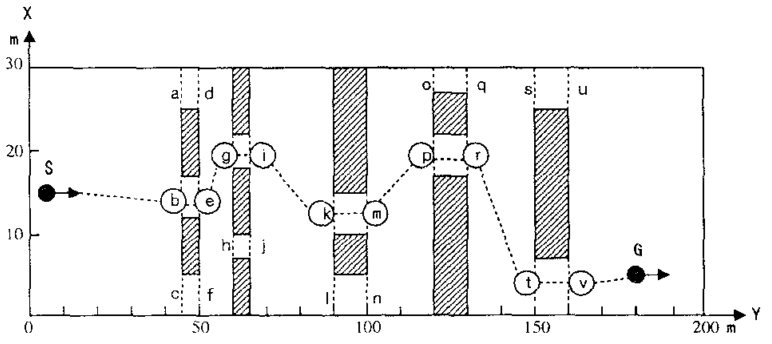
\includegraphics[width=.55\linewidth]{GridBasedLocalConstrAUV-a}} \quad
    \subfloat[] 
    {\label{fig:GridBasedLocalConstrAUV-b}
     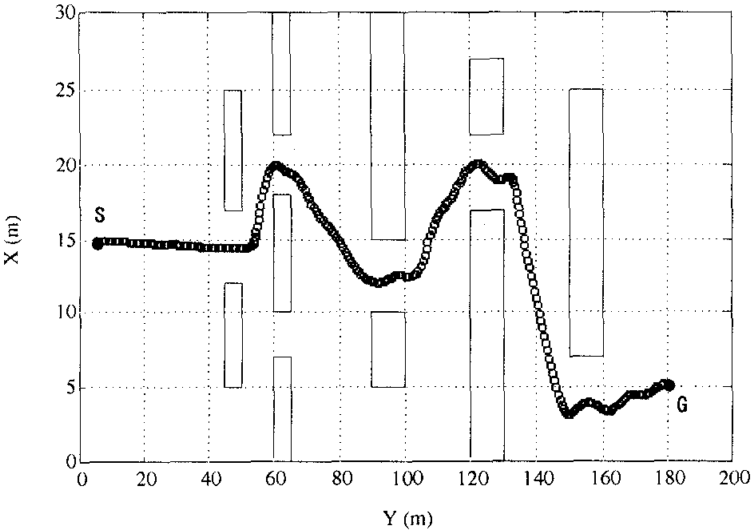
\includegraphics[width=.4\linewidth]{GridBasedLocalConstrAUV-b}}
\caption[Combination of a grid-based planning method and a local planner
to include the AUV motion constraints.]
{\protect \subref{fig:GridBasedLocalConstrAUV-a} Global motion planning solved
by a grid-based method, \protect \subref{fig:GridBasedLocalConstrAUV-b} which is
adjusted by a local planner that takes into consideration the AUV motion
constraints. Image credit: Arinaga \etal\cite{Arinaga1996}.}
\label{fig:GridBasedLocalConstrAUV}
\end{figure}

A third group of recent contributions includes those that use sampling-based
planning algorithms. The most common approach builds a tree of collision-free
configurations, which are obtained by integrating the differential equation that
describes the \ac{AUV} dynamic behavior~\cite{Tan2004,Caldwell2010,Heo2013}.
This strategy was briefly introduced in
Section~\ref{sec:motion_constraints_review}, but its use with a torpedo-shaped
\ac{AUV} will be explained in more detail in
Chapter~\ref{ch:motion_constratins}.

Finally, there is another concept for generating feasible paths. It consists in
utilizing the Dubins curves~\cite{Dubins1957}, which establishes a set of six
maneuvers (RSR, RSL, LSR, LSL, RLR, LRL, where R states for Right, L for Left,
and S for straight) to connect two configurations $q_i,q_j \in \mathcal{C} =
SE(2)$. These curves correspond to time-optimal trajectories for car-like
vehicles. Albeit they have been used for trajectory
generation~\cite{Wehbe2014,Cao2016}, they are also useful in the context of this
thesis.
% , as it will be explained in more detail in
% Section~\ref{sec:2d_motion_constratins}.

% Finally, there is a geometric alternative to generate feasible paths for
% motion-constrained \acp{AUV}. It consists in utilizing the Dubins
% paths~\cite{Dubins1957}, which establishes a set of six maneuvers (RSR, RSL,
% LSR, LSL, RLR, LRL, where R states for Right, L for Left, and S for straight) to
% connect two configurations $q_i,q_j \in \mathcal{C} = SE(2)$.  These paths
% correspond to time-optimal trajectories for car-like vehicles, and they have
% also been used more recently with some underwater
% vehicles~\cite{Wehbe2014,Cao2016}. However, in this latter case, the Dubins
% paths have worked more as a trajectory planner, rather than a path planner with
% online obstacle avoidance capabilities. Further discussion of Dubins maneuvers
% and their use with \acp{AUV} will be presented throughout
% Section~\ref{sec:2d_motion_constratins}.

% \begin{figure}[htbp]
%     \myfloatalign
%     \subfloat[]
%     {\label{fig:Dubins3DGlidersConstrAUV-a}
%     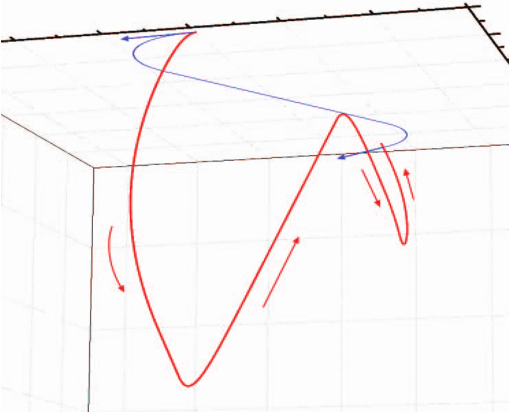
\includegraphics[width=.45\linewidth]{Dubins3DGlidersConstrAUV-a}} \quad
%     \subfloat[] 
%     {\label{fig:Dubins3DGlidersConstrAUV-b}
%      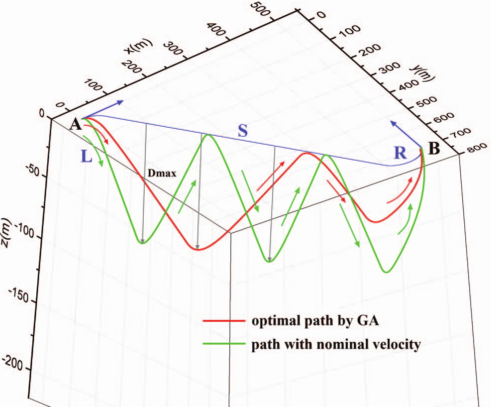
\includegraphics[width=.45\linewidth]{Dubins3DGlidersConstrAUV-b}}
% \caption[Glider trajectory planner combining the Dubins curves and
% sinusoidal-like vertical motion.]
% {\protect \subref{fig:Dubins3DGlidersConstrAUV-a} Glider trajectory planner that
% combines the Dubins curves and the sinusoidal-like vertical motion.
% \protect \subref{fig:Dubins3DGlidersConstrAUV-b} A genetic algorithm calculates
% the optimal trajectory for a glider that moves in obstacle-free environment.
% Image credit: Cao \etal\cite{Cao2016}.}
% \label{fig:Dubins3DGlidersConstrAUV}
% \end{figure}

% \subsection{Online Mapping and Path/Motion Planning}
Another characteristic required for the new \ac{AUV} applications is the
capability of mapping and planning safe paths, simultaneously and online, as the
environment is incrementally explored. Apart from the already explained work by
Petillot et al., which in fact does not demonstrate online mapping and planning
capacity~\cite{Petillot2001}, Maki \etal~proposed an online motion planning
method that uses landmarks to guide an \ac{AUV}. Nonetheless, their approach does not
permit replanning and, furthermore, results were obtained in a controlled
environment (\ie in a water tank)~\cite{Maki2007}.

\section{Summary}

This chapter has presented an extensive review of the most common path/motion
planning approaches, and those that have been used with underwater vehicles.
Table~\ref{table:SummaryPlanningMethdos} presents a summary of such methods and
their characteristics. It is important to bear in mind that the intended
applications for \acp{AUV}, discussed in Chapter~\ref{ch:introduction}, must
meet online computation constraints in order to deal with unexplored
environments. This implies that time complexity and anytime computation are
important requirements. The following chapters will present the extension of
some of these approaches, and their successful use in some of the intended
applications introduced in Chapter~\ref{ch:introduction}.

\begin{table}[htbp]
\begin{center}
\begin{tabular}{ l c c c c }
  \hline
  \hline
  Method & Completeness & Optimality & Time Complexity & Anytime \\ \hline \hline
  \multicolumn{5}{c}{\textbf{Search-based}}\\ \hline
  Dijkstra & Yes$^{a}$ & Yes & $O(n^2)^{a}$ & No \\ \hline
  A* & Yes & Yes & $O(b^d)^{b}$ & No$^b$ \\ \hline
  \multicolumn{5}{c}{\textbf{Potential fields}}\\ \hline
  \makecell[l]{Potent. \\ Funct.} & No$^c$ & Locally & $O(1)$ & Yes
  \\ \hline \multicolumn{5}{c}{\textbf{Roadmaps}}\\ \hline
  \makecell[l]{Visibility \\Graphs} & Yes & Yes$^d$ & $O(n^2)^d$ & No \\ \hline
  \multicolumn{5}{c}{\textbf{Sampling-based}}\\ \hline
  \makecell[l]{PRM +\\ Dijkstra} & Prob. Compl. & Asymp. Opt. & $O(n^2)^e$ &
  No \\
  \hline RRT & Prob. Compl. & No & $O(n \log n)^e$ & Yes \\ \hline
  RRT* & Prob. Compl. & Asymp. Opt. & $O(n \log n)^e$ & Yes \\ \hline
%   1 & 2 & 3 \\ \hline
%   4 & 5 & 5  \\ \hline
%   7 & 8 & 9 \\ \hline
\end{tabular}
\end{center}
\caption[Path/motion planning methods.]
{Path/motion planning methods. $^{a}$ Complete for bounded \ac{C-Space}, where n
is the number of nodes in the graph. $^{b}$ The number of nodes expanded is
exponential in the depth of the solution, where \textit{b} is the branching
factor (the average number of successors per state); ARA* provides a mechanism
for anytime computation by reusing previous solutions. $^c$ requires full
knowledge of the \ac{C-Space}, suffers form local minima. $^d$ Optimal with
respect to the traveled distance; where $n$ is the number of points defining
obstacles. $^e$ Number of sampled configurations.}
\label{table:SummaryPlanningMethdos}
\end{table}



% ---------------------------------------------------------------------------
% ----------------------- end of thesis sub-document ------------------------
% ---------------------------------------------------------------------------
%\cleardoublepage
%% this file is called up by thesis.tex content in this file will be fed into the
% main document

% : ----------------------- name of chapter  -------------------------
\chapter{Planning Constant-Depth Paths under AUV Motion Constraints}
\label{ch:motion_constratins}
% top level followed by section, subsection


% : ----------------------- paths to graphics ------------------------

% change according to folder and file names
\ifpdf
    \graphicspath{{3_motion_constraints/figures/PNG/}{3_motion_constraints/figures/PDF/}{3_motion_constraints/figures/}}
\else
    \graphicspath{{3_motion_constraints/figures/EPS/}{3_motion_constraints/figures/}}
\fi

% : ----------------------- contents from here ------------------------

% As explained in Section~\ref{sec:motion_constraints_review}, planning problems
% for robotic systems can be categorized in one of the two groups:
% \begin{inparaenum}[1)] \item path planning, which refers to those problems that
% only consider geometric constraints, and \item motion planning for those that
% also consider the kinematic and/or dynamic aspects of the system.
% \end{inparaenum}
% However, some authors use the latter term to refer to either
% group~\cite{Sucan2011},~\cite{LaValle2006}. Throughout this thesis, both terms
% are used interchangeably, nonetheless there will be a special emphasis when
% referring to the motion constraints involved, since they have been a determining
% aspect in meeting the proposed objectives.

Recent and potential applications for \acp{AUV} mentioned in
Chapter~\ref{ch:introduction} establish most of the motion planner requirements,
such as online computation, motion in \ac{3D} workspaces, and navigation along
unexplored environments in close-proximity to nearby obstacles. All these
constraints can be met with sampling-based planning methods. Particularly for
navigating in close-proximity, one desired characteristic is being able to
calculate feasible motions that take into account the \ac{AUV}
capabilities. This allows minimizing unexpected vehicle trajectories when
attempting to follow the calculated path. In this respect, this chapter firstly
explains the equations of motion used to approximate the \ac{2D} (at a constant
depth) vehicle behavior for motion-planning purposes. Secondly, it explains two
different approaches to integrate such equations into the motion planner.
Lastly, it presents and discusses the results obtained with both approaches in a
simulated environment.

\section{2D First-Order Motion Model}
\label{sec:2d_kinematic_model}

As occurs with any mechanical system, \ac{AUV} motions can be formulated with
kinematic and dynamic models. The former ones describe the geometry of motion by
relating the system positions and velocities. Dynamic models, on the other
hand, not only include the system kinematics, but also take into account the
forces and torques that generate the motions. This latter kind of model is
generally employed for designing robust controllers, however, their high
computational cost makes them an inappropriate approach for the scenarios
proposed in this thesis, which require an online (re)planning behavior. The
associated overhead is especially true when using sampling-based planning
methods, where all configurations are generated by evolving the system, \ie
performing numerical integration of the equation of motion. Alternatively, a
kinematic model provides a less accurate approximation for the vehicle's motion
constraints, but it also allows additional computation time that can be
dedicated to finding better collision-free paths.

In order to establish which kinematic model must be used, it is necessary to
understand the vehicle motion capabilities and the possible test scenarios. In
some \ac{AUV} applications, a first valid approximation is to assume that the
vehicle navigates at a constant depth (see
Sec.~\ref{sec:StateOfTheArtPlannAUV}). Furthermore, if the vehicle is a
torpedo-shaped \ac{AUV}, usually, it will only be able to changing its direction
of motion by moving forward/backward. In the case of the Sparus~II \ac{AUV}, the
vehicle is equipped with two back thrusters that allow it to spin over. However,
it is still not capable of conducting lateral motion. Therefore, it is correct
to affirm that the vehicle is subject to a motion constraint along its y-axis
(see Fig.~\ref{fig:RefFramesAUV2D}).

As explained in Chapter~\ref{ch:introduction}, motion or differential
constraints can be expressed as a set of differential equations in the general
form $\dot{q}=f\left(q,u\right)$, where $q$ and $\dot{q}$ are the system state
and its first derivative, respectively, and $u$ is the control input.
Having this in mind, and considering the aforementioned constraints when
navigating at a constant depth, a non-holonomic and torpedo-shaped \ac{AUV} can
be represented as a simple car-like vehicle, with a first-order motion model
defined as follows:

\begin{equation}
\label{eq:KinEqAUV2D}
	\begin{bmatrix}
		\dot{x}\\
		\dot{y}\\
		\dot{\psi}\\
	\end{bmatrix}=
	\begin{bmatrix}
		v\ cos\left(\psi\right) \\
		v\ sin\left(\psi\right)\\
		w\\
	\end{bmatrix}
	\text{,}
\end{equation}

where $q=\left[x, y, \psi\right]^T$ corresponds to the system state that
includes its \ac{2D} position and orientation with respect to an inertial
reference frame, and $\dot{q}=\left[\dot{x}, \dot{y}, \dot{\psi}\right]^T$ is
the first time derivative that depends on the state itself and the control
inputs, \ie linear/surge speed ($v$) and turning rate ($w$). From
Eq.~\eqref{eq:KinEqAUV2D}, it can be concluded that the \ac{C-Space} of a
torpedo-shaped \ac{AUV} is $\mathcal{C} = SE(2) = \mathbb{R}^2 \times SO(2) =
\mathbb{R}^2 \times \mathcal{S}$. Figure~\ref{fig:RefFramesAUV2D} depicts the
inertial frame, the body-fixed frame, and the different variables (positions and
velocities) contained in~\eqref{eq:KinEqAUV2D}.

\begin{figure}[htbp]
	\centering
	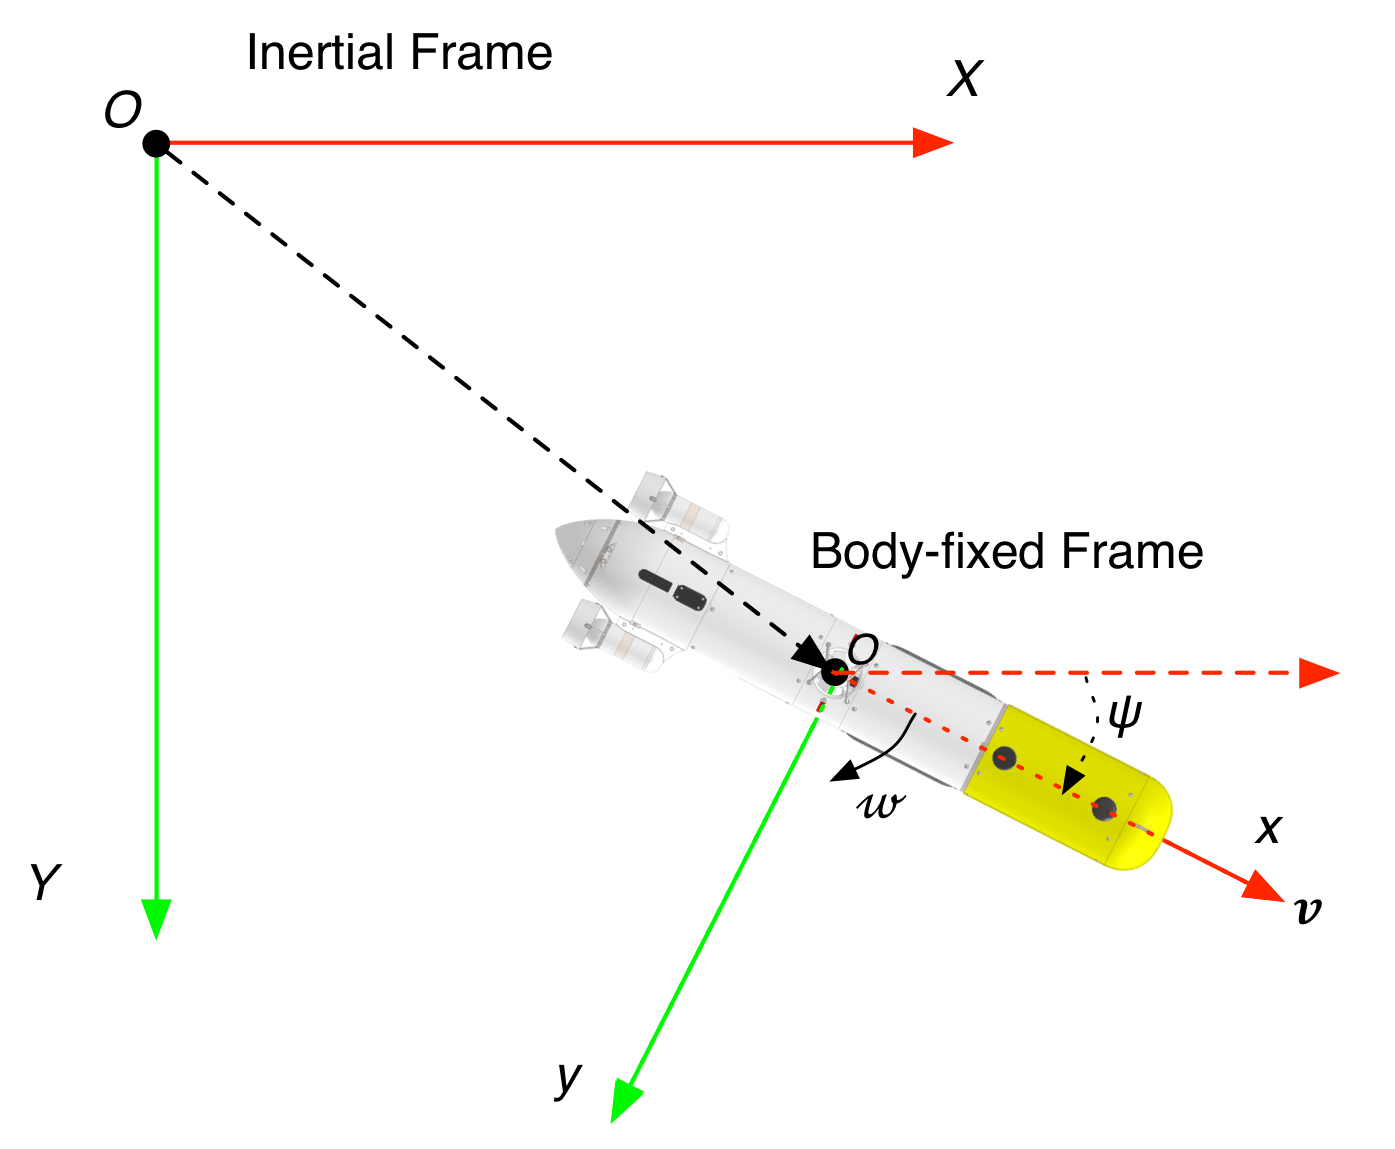
\includegraphics[width=.7\linewidth]{RefFramesAUV2D} \quad
	\caption[Top view of the Sparus~II AUV, including the inertial and body-fixed
	frames, and the 2D vehicle state and control variables.]
	{Top view of the Sparus~II AUV, including the inertial and body-fixed
	frames, and the 2D vehicle state and control variables.}
	\label{fig:RefFramesAUV2D}
\end{figure}

Once the constraints have been established through the corresponding
differential equations, the next step is to define an appropriate strategy to
generate feasible motions that meet such constraints. The following
sections present two different approaches, which use sampling-based algorithms
to calculate such kind of motions for a torpedo-shaped \ac{AUV} that navigates
at a constant depth.

\section{Motion Planning by Using Differential Equations}
\label{sec:expan_2d_diff_eq}

% Although some of the classical grid-based methods have addressed the problem of
% planning motions under differential constraints (see
% Sec.~\ref{sec:motion_constraints_review}), those approaches establish a grid
% over the \ac{C-Space} and define a finite set of possible maneuvers, thus
% reducing the number of viable solutions. On the other hand, 
Sampling-based algorithms, especially the \ac{RRT}~\cite{LaValle2001} and its
variants, have proved to efficiently explore the \ac{C-Space} while taking all
the motion constraints into account. Furthermore, there are other
characteristics such as the incremental search behavior, which allows these
methods to continuously (re)plan the solution path as the vehicle moves through
unexplored environments (see Chapter~\ref{ch:plann_online}). All this together
makes an \ac{RRT}-based algorithm the appropriate approach for the intended
\ac{AUV} applications.

As explained in Section~\ref{sec:RRT}, the \ac{RRT} algorithm builds a single
tree that is rooted at an initial state (configuration), which is incrementally
expanded towards uniformly randomly \textit{sampled} states\footnote{There
exists another RRT variant called RRT-Connect that grows two trees, one from the
start state and another one from the goal state. However, this is not possible
when dealing with motion constraints, since merging both trees at a common
configuration may become computationally intractable~\cite{Kuffner2000}.}. This
procedure is the same as the one initially presented in
Algorithm~\ref{alg:SampleRRT}, being this a particular case where a random state
corresponds to $q_{rand}\in SE(2)$, as explained before. In order to
\textit{extend} the tree towards $q_{rand}$ while meeting the vehicle's motion
constraints, new collision-free motions (states) are obtained by integrating the
vehicle's equation of motion, such as Eq.~\eqref{eq:KinEqAUV2D}. In such a case,
instead of using Algorithm~\ref{alg:ExtendRRT}, the tree expansion can be
rewritten as shown in Algorithm~\ref{alg:ExtendRRTDiffConstr}. This procedure
firstly requires finding the state $q_{near}$, that is the nearest to $q_{rand}$
(line~\ref{alg_line:findNearest}). This can be done by using a weighted metric
to calculate the distance between configurations. Such a metric combines the
translation component, calculated as the Euclidean distance, and the orientation
component, calculated as the smallest orientation
difference~\cite{Choset2005,LaValle2006}.

\begin{algorithm}[htbp]
\DontPrintSemicolon

	\SetKwFunction{calcNewState}{calcNewState}
	\SetKwFunction{findNearestNeighbor}{findNearestNeighbor}
	\SetKwFunction{addNewNode}{addNewNode}
	\SetKwFunction{addNewEdge}{addNewEdge}
	\SetKwFunction{findInput}{findInput}
	
	\KwIn{\\ 
	$T$: tree of collision-free configurations.\\ 
	$q_{rand}$: configuration towards which the tree will be extended.\\
 	$\mathcal{C}$: \ac{C-Space}.}
	\KwOut{\\ Result after attempting to extend.}
	\Begin{
	 	$q_{near}\leftarrow T.$\findNearestNeighbor{$q_{rand}$}\;\label{alg_line:findNearest}
	 	$u_{near\_ to\_rand}\leftarrow$\findInput{$T,q_{near},q_{rand}$}\;\label{alg_line:findInput}
	 	$q_{new}, collision\leftarrow$\calcNewState{$q_{near},u_{near\_to\_rand},\Delta t$}\;\label{alg_line:calNewState}
	 	\If{$collision = FALSE$} {\label{alg_line:ifCollision} 
	 		V.\addNewNode{$q_{new}$}\;
	 		E.\addNewEdge{$q_{near},q_{new}$}\;\label{alg_line:addNewEdge}
	 	}
 	}
\caption[extendRRT when dealing with motion constraints.]
{extendRRT (when dealing with motion constraints)}
\label{alg:ExtendRRTDiffConstr}
\end{algorithm}

Once the nearest motion has been found in the tree, the next step is to
calculate the control input $u_{near\_ to\_rand}=\left[v, w\right]$ that has to
be applied in order to change the vehicle state from $q_{near}$ towards
$q_{rand}$ (line~\ref{alg_line:findInput}). With an \ac{RRT} algorithm under
geometric constraints the tree is iteratively expanded a geometric distance
$\epsilon$ (see Algorithm~\ref{alg:ExtendRRT},
line~\ref{alg_line:ExtendRRTGeom}), in the case of an \ac{RRT} algorithm under
motion constraints the tree is expanded by applying an input $u$ for a period of
time $\Delta t$ (line~\ref{alg_line:calNewState}).

In some \ac{AUV} applications, a common assumption is that the vehicle navigates
at a constant surge speed $v$, but can vary its turning rate $w$ up to a maximum
value $w_{max}$. This means that calculating the input $u$ is limited to firstly
establishing a constant $v$ that will be used along the mission, and then
computing a valid value for $w$ that meets the vehicle motion constraints. There
are different approaches that permit calculating $u$. Two alternatives, also
presented by LaValle and Kuffner~\cite{LaValle2001}, are either to randomly
sample the control space, or to test a number of possible inputs and then select
the one that generates the state $q_{new}$ that is closest to $q_{rand}$. The
implementation used in a first stage of this thesis is based on a combination of
both approaches.

In such an implementation, instead of testing a large number of different
turning rates $w$, a set of five possible values is established as
follows: $w_{control_i} \in \left\{-w_{max}, -\frac{w_{max}}{2}, 0,
\frac{w_{max}}{2}, w_{max}\right\}$. These values, in turn, define a
set of four sub-intervals over the control space:
%
$\{[-w_{max}, -\frac{w_{max}}{2}],$ $[-\frac{w_{max}}{2}, 0],
[0, \frac{w_{max}}{2}], [\frac{w_{max}}{2}, w_{max}]\}$.
%
Then, using Eq.~\eqref{eq:KinEqAUV2D} with $q_{near}$ as the starting state, each
$u_i = \left[v, w_{control_i}\right]$ is applied for a period of time $\Delta t$
to generate five different states $q_{control_i}$. Having them, it is possible
to estimate which of the four sub-intervals may contain a control input that
leads the tree expansion from $q_{near}$ closer to $q_{rand}$. The final value
of $w_{rand}$ is obtained by sampling a random turning rate over the chosen
sub-interval. This procedure avoids discretizing the control space, which would
imply the loss of the random exploration of the \ac{C-Space}, an important
property of the original algorithm. Figure~\ref{fig:ControlInputSampling}
presents the main concept of the control input selection.

\begin{figure}[htbp]
	\centering
	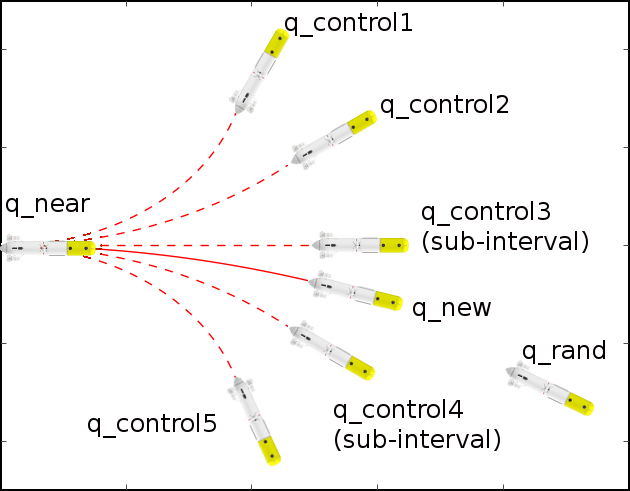
\includegraphics[width=.6\linewidth]{ControlInputSampling} \quad
	\caption[Control input selection for expanding an RRT under the differential
	equation.]
	{Control input selection. Tree is expanded from $q_{near}$ towards
	$q_{rand}$. To do so, an interval of possible turning rates ($q_{control\_i}$)
	are evaluated. This permits defining a sub-interval from which the control
	input is sampled randomly, and is applied to generate the new state
	$q_{new}$.}
	\label{fig:ControlInputSampling}
\end{figure}

The remaining of the \textit{extend} procedure
(Algorithm~\ref{alg:ExtendRRTDiffConstr}) calculates the new state $q_{new}$
(line~\ref{alg_line:calNewState}). This is done by integrating
Equation~\eqref{eq:KinEqAUV2D} while using the final sampled input $u_{near\_
to\_rand} = \left[v, w_{rand}\right]$. Finally, if $q_{new}$ is proved to be
collision-free, it is added and connected to the tree
(lines~\ref{alg_line:ifCollision}-\ref{alg_line:addNewEdge}).
Figure~\ref{fig:RRTDiffConstr} depicts an example of an \ac{RRT} algorithm that
solves a start-to-goal query under these motion constraints.

\begin{figure}[htbp]
    \myfloatalign
    \subfloat[]
    {\label{fig:RRTDiffConstrStep1}
    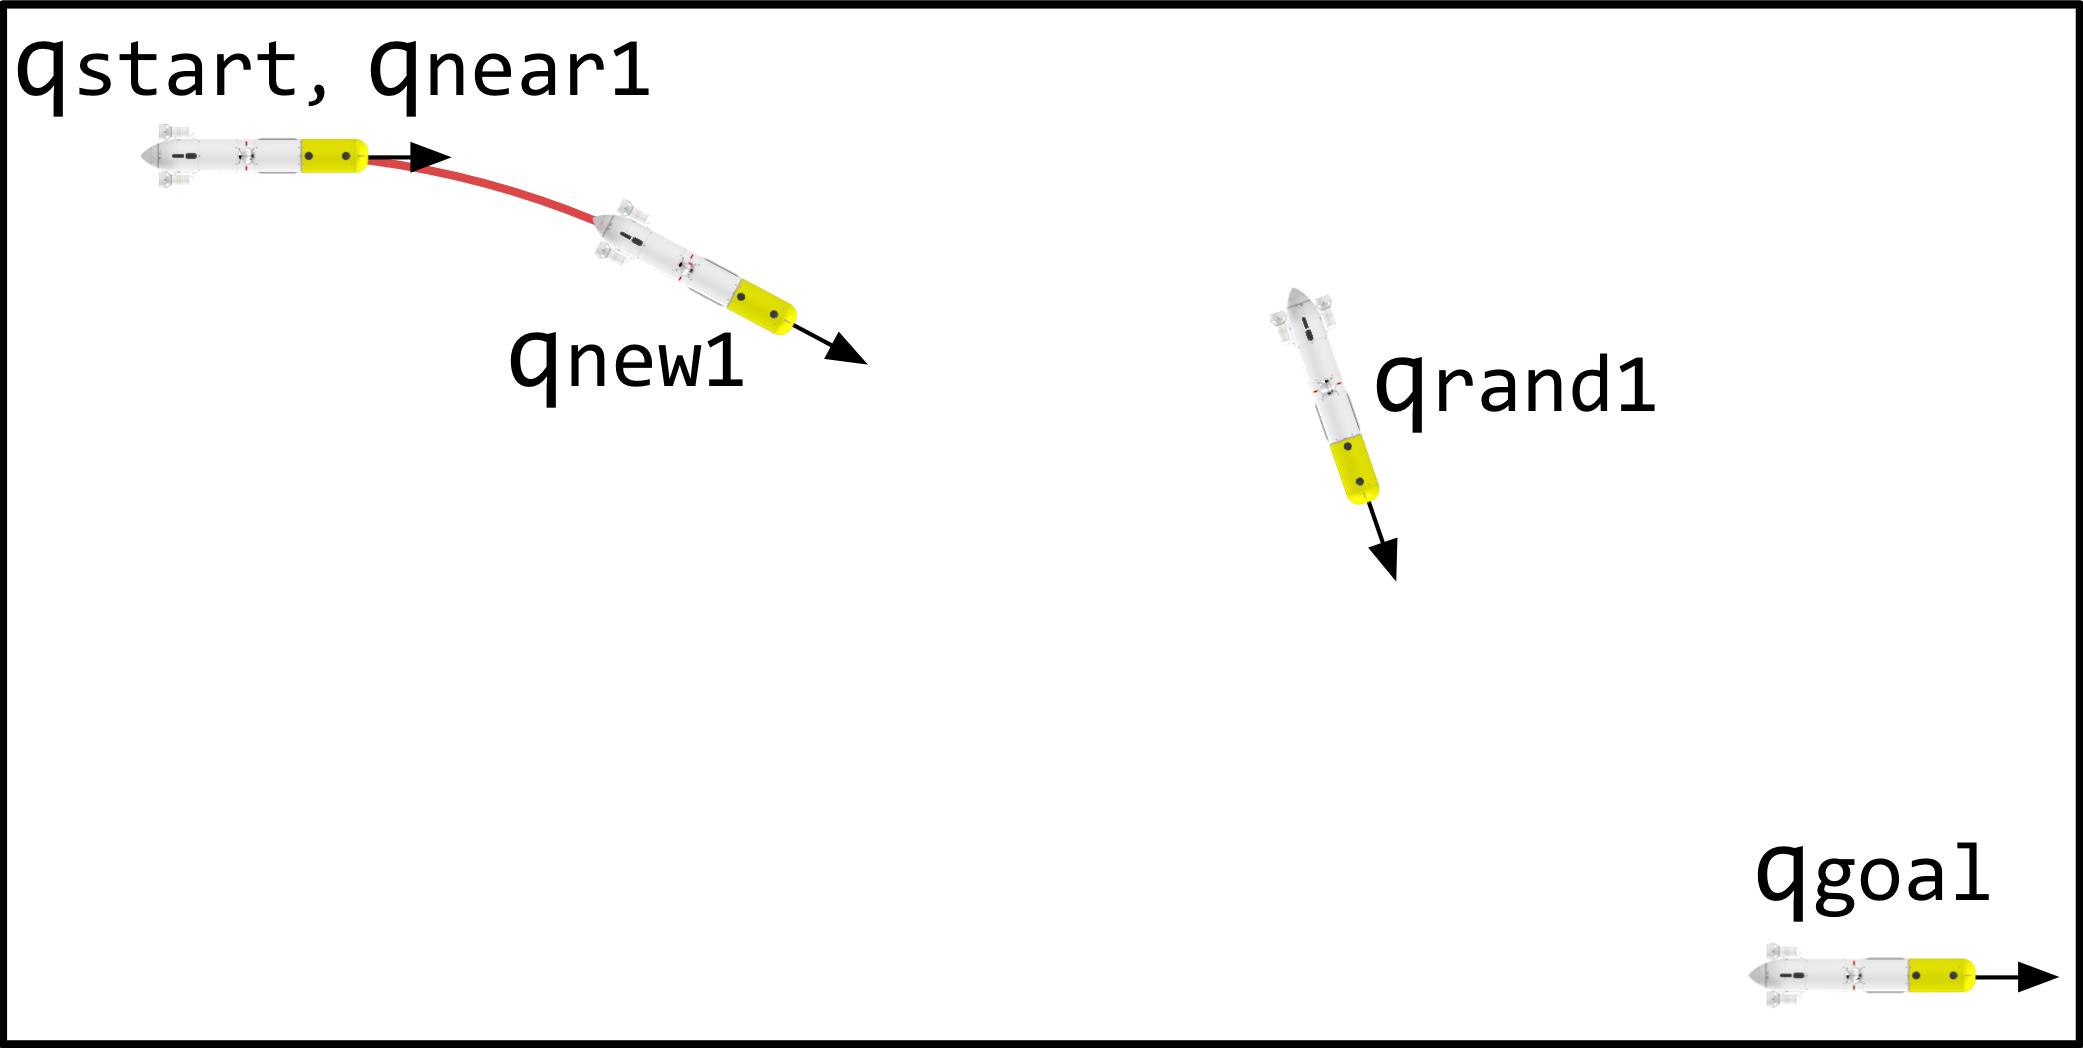
\includegraphics[width=.42\linewidth]{ExpansionRRTDiff-a}} \quad
    \subfloat[]
    {\label{fig:RRTDiffConstrStepi}%
     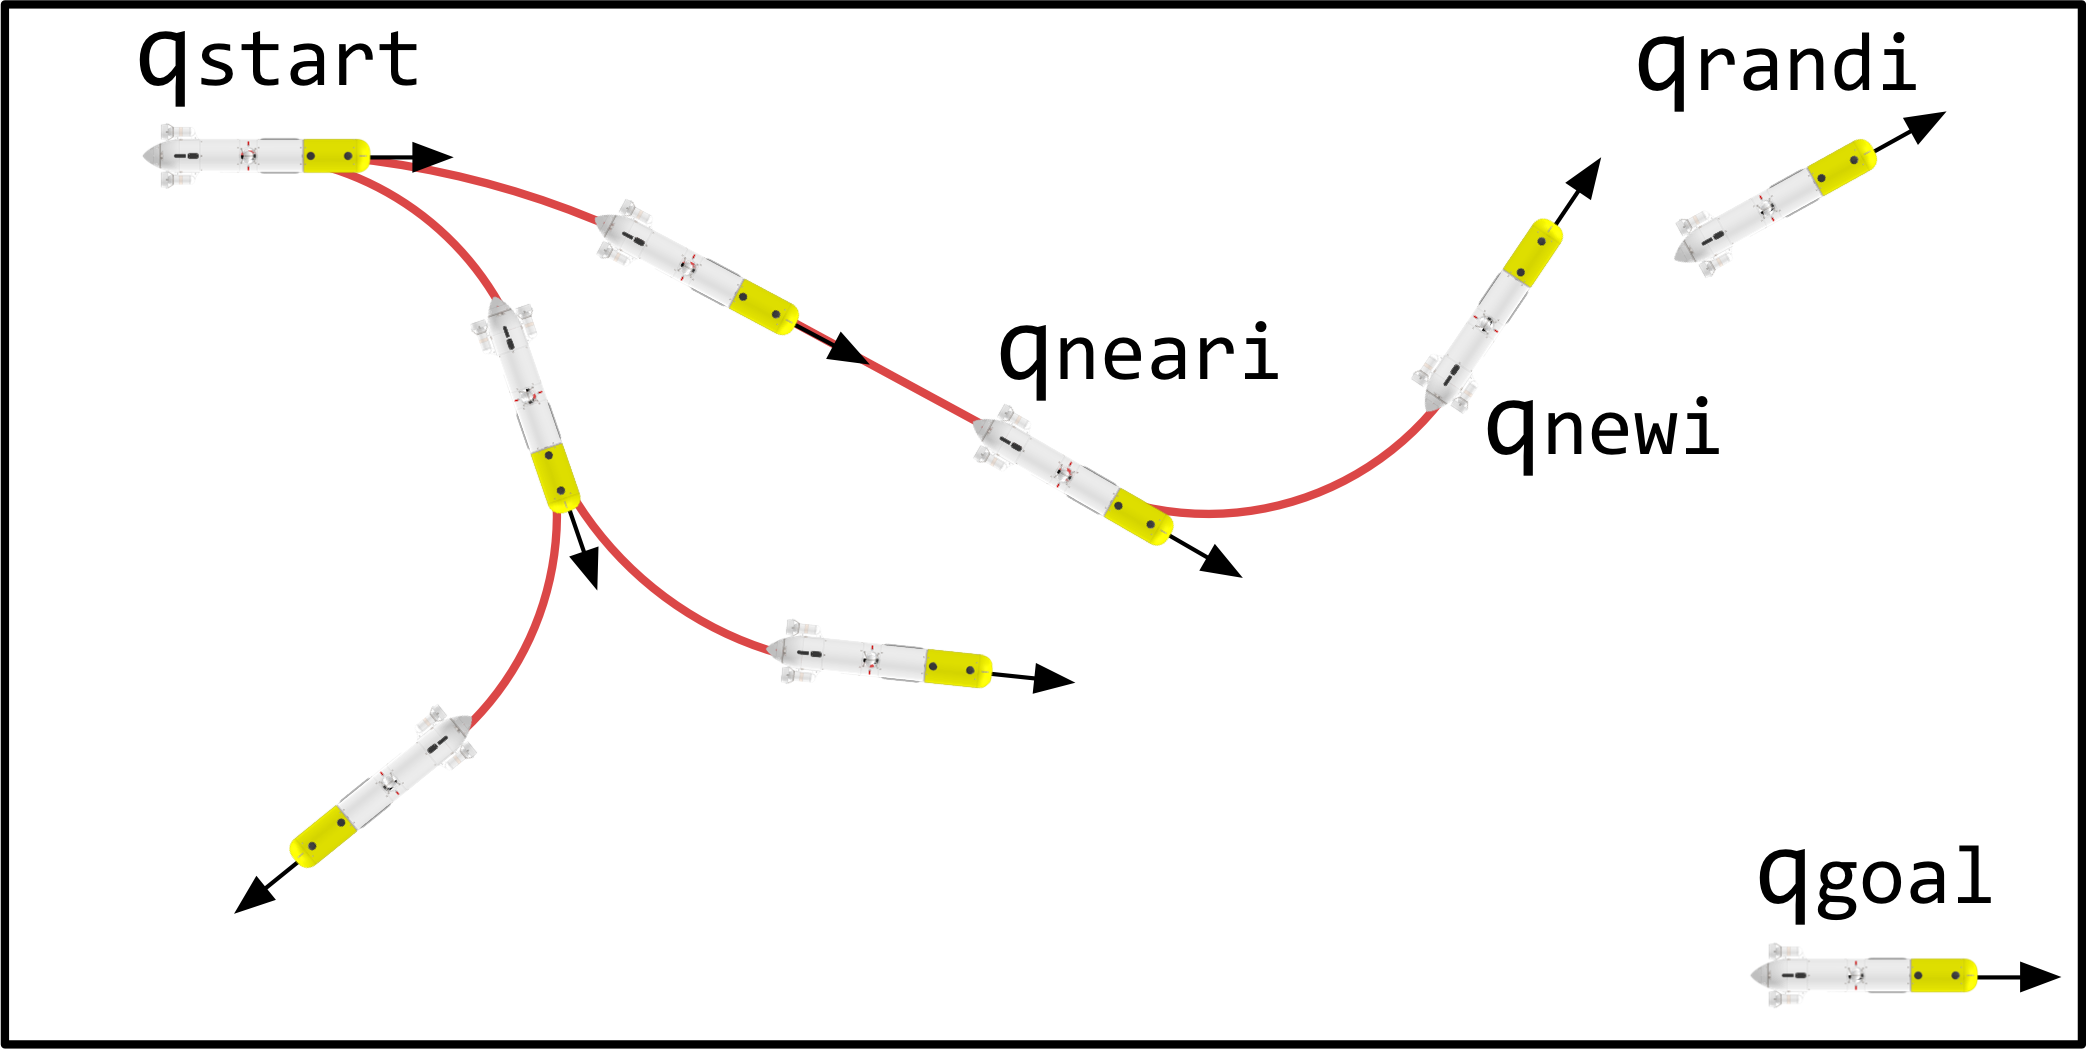
\includegraphics[width=.42\linewidth]{ExpansionRRTDiff-b}} \quad
    \subfloat[]
    {\label{fig:RRTDiffConstrComplete}
    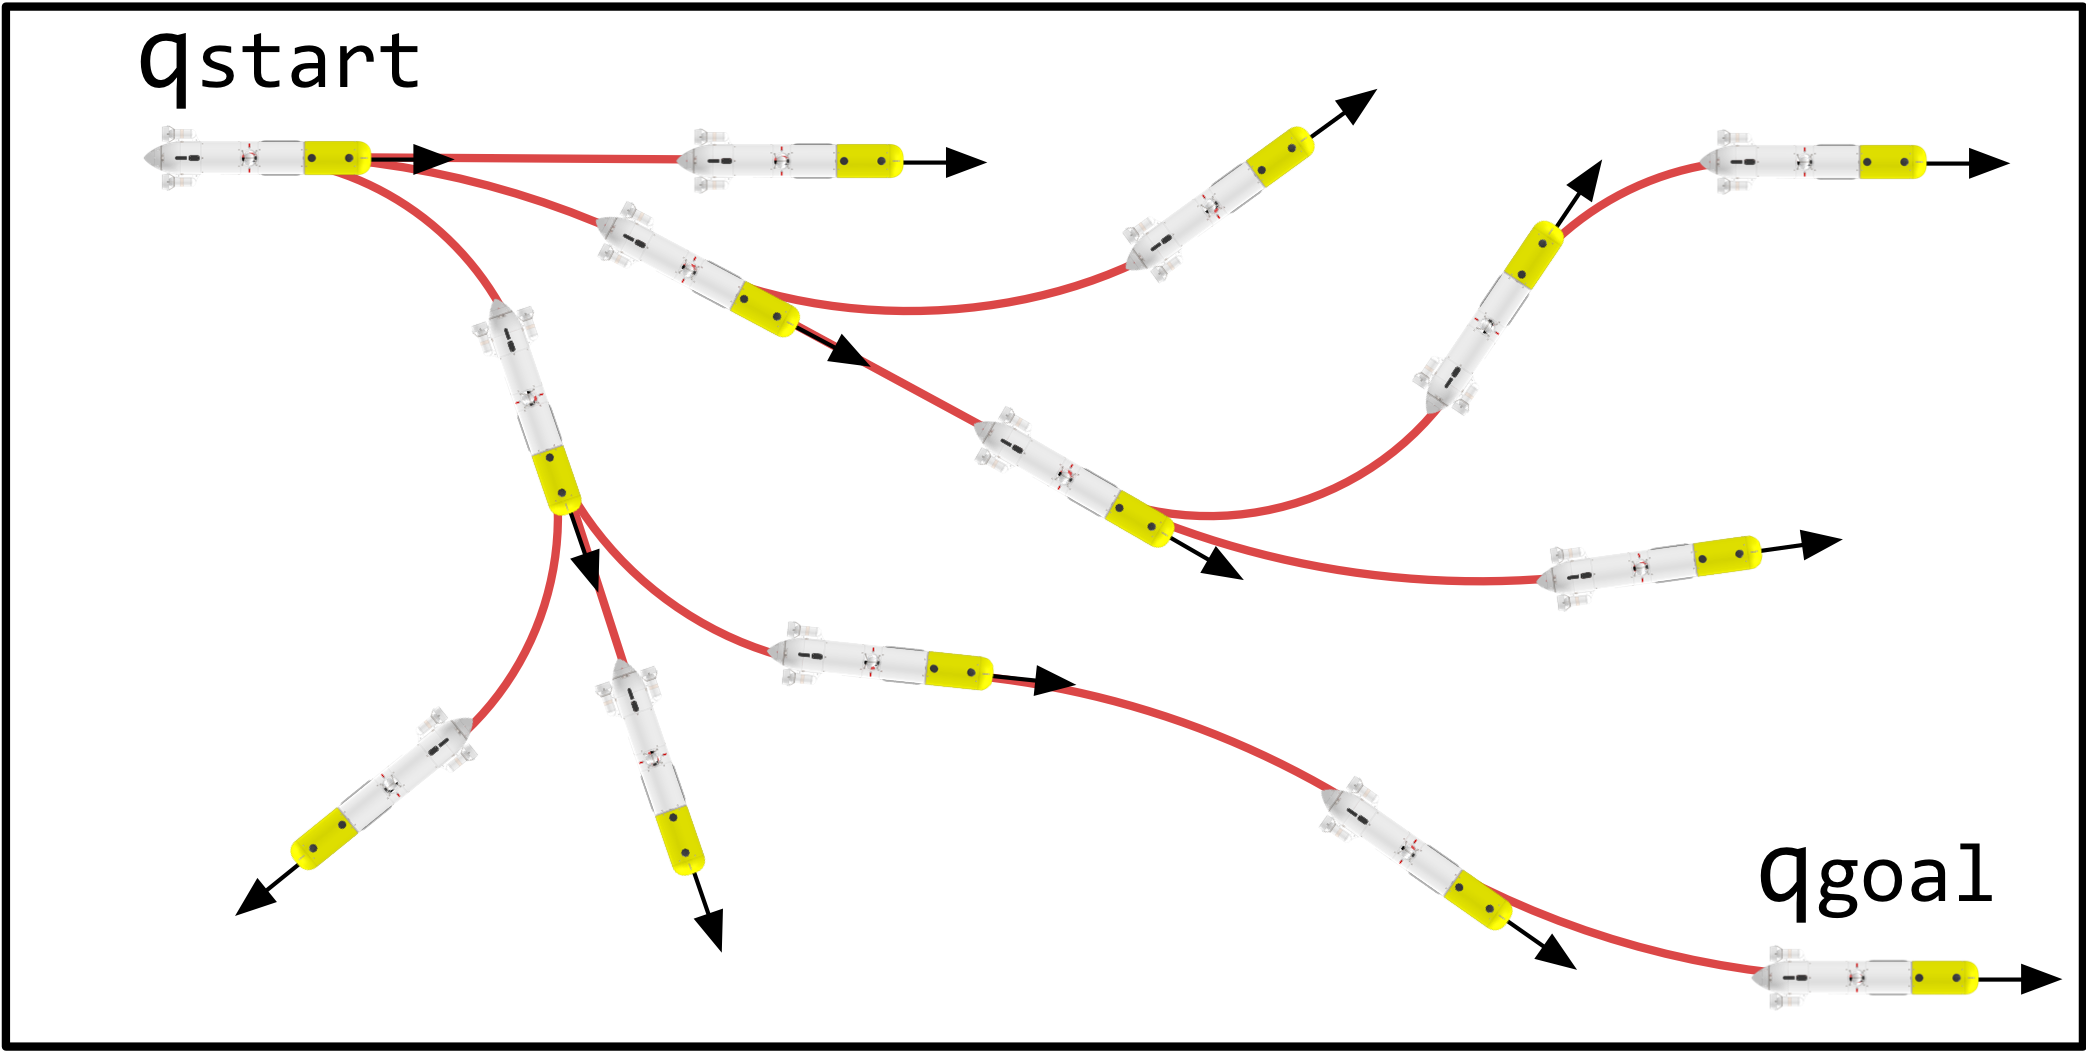
\includegraphics[width=.42\linewidth]{ExpansionRRTDiff-c}}
\caption[Start-to-goal query solution by expanding an RRT algorithm that
considers the differential constraints of a car-like system.]
{Tree expansion of an \ac{RRT} algorithm that considers the differential
constraints described by Equation~\eqref{eq:KinEqAUV2D}.
\protect \subref{fig:RRTDiffConstrStep1} Given the start and goal states, a
first random sample is used to generate the first expansion of the tree
($q_{new}$).
\protect \subref{fig:RRTDiffConstrStepi} The expansion $i^{th}$ of the tree.
\protect \subref{fig:RRTDiffConstrComplete} A feasible path has been found from
the start to the goal state.}
\label{fig:RRTDiffConstr}
\end{figure}

%\cleardoublepage

\section{Motion Planning by Using Dubins Curves}
\label{sec:expan_2d_dubins}

There are several examples where a purely geometric path is first computed, and
then it is transformed into a path that is appropriate for the considered
vehicle. For example, Yang \etal used an \ac{RRT} algorithm to find a route of
collision-free waypoints, which is interpolated with a cubic B\'ezier
spiral~\cite{Yang2008}. This seeks to convert the initial route into a smooth
and feasible path for an \ac{UAV}. As another example, Kuwata \etal proposed to
expand an \ac{RRT} by considering not only the vehicle dynamics, but also its
controller behavior~\cite{Kuwata2009}.

There are other \ac{RRT}-based approaches that have been proposed to generate
feasible paths for aerial and terrestrial vehicles. In one of those approaches,
for instance, a geometric \ac{RRT} algorithm finds a route of collision-free
waypoints, which are interpolated with a cubic B\'ezier spiral. This seeks to
convert the initial route into a smooth and feasible path for an
\ac{UAV}~\cite{Yang2008}. In another approach that is closer to the one
presented in the previous section, an \ac{RRT} algorithm is expanded by
considering not only the vehicle dynamics, but also its controller
behavior~\cite{Kuwata2009}.

Nonetheless, all those approaches, including the one presented in the previous
section, have a major drawback; they do not guarantee optimality for any metric.
It is a common characteristic of most sampling-based methods, at least in their
original form. This issue could be critical in underwater applications, which
may require optimizing different criteria such as visibility (for gathering
information), vehicle autonomy, or even the safety associated with a path when
navigating in close-proximity to nearby obstacles.

As explained in Section~\ref{sec:SamplOptimalPlan}, one option to cope with this
situation is to use the \ac{RRT*} algorithm, which is a variant that
incorporates the asymptotic optimality property~\cite{Karaman2011}.
Its main difference with respect to other \ac{RRT}-based methods, is a routine
that checks if reconnecting new state's nearest nodes improves their associated
cost. This implies that the probability of obtaining an optimal path converges
to 1 over time. (see Algorithm~\ref{alg:ExtendRRTstar}). For doing this, the
\ac{RRT*} algorithm requires a steering function that permits calculating such
states (nodes) reconnection. In the case of systems under motion constraints,
having such a function implies calculating the required input to dynamically
evolve the system from a given state to a desired one. However, defining this
function requires solving a two-point boundary value problem, which is in
general a very difficult problem.

For the purposes of this thesis, as an alternative to defining a steering
function, it is possible to adopt the Dubins vehicle model~\cite{Dubins1957}.
Dubins geometrically demonstrated that, for a system that is only capable of
traveling forward and with a constraint on the curvature of the path, the
shortest path to connect any two configurations (states) $q_i,q_j \in SE(2)$,
when no obstacles are present, can be obtained analytically by the combination
of circular arcs and straight lines. Using three possible maneuvers as input,
left (L), straight (S) or right (R), Dubins curves define six possible
combinations: RSR, RSL, LSR, LSL, RLR, LRL. For a Dubins vehicle, at least one
of these characterizes the optimal (shortest) trajectory between two states (see
Fig.~\ref{fig:DubinsPathsExample}).

\begin{figure}[htbp]
    \myfloatalign
    \subfloat[RSL]
    {\label{fig:DubinsRSL}
    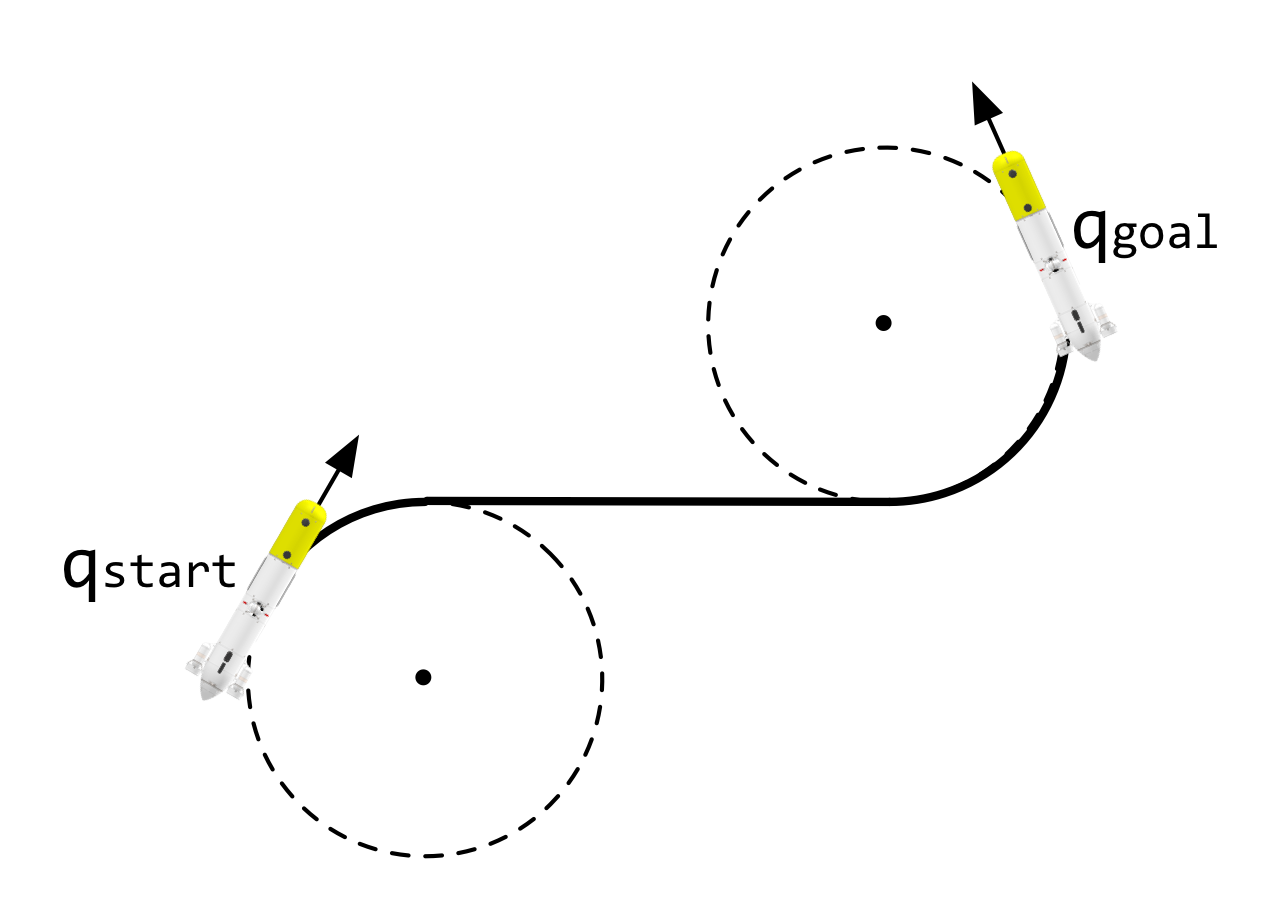
\includegraphics[width=.45\linewidth]{DubinsRSL}} \quad
%     \subfloat[RSR]
%     {\label{fig:DubinsRSR}%
%      \includegraphics[width=.45\linewidth]{DubinsRSR}}\\%\quad
%     \subfloat[RLR]
%     {\label{fig:DubinsRLR}
%     \includegraphics[width=.35\linewidth]{DubinsRLR}} \qquad
    \subfloat[LRL]
    {\label{fig:DubinsLRL}%
     \includegraphics[width=.33\linewidth]{DubinsLRL}}
\caption[Examples of Dubins curves.]
{Examples of Dubins curves}
\label{fig:DubinsPathsExample}
\end{figure}

These constrained maneuvers are commonly used to describe feasible trajectories
for different ground, aerial, and underwater vehicles such as a torpedo-shaped
\ac{AUV}. For this latter case, Equation~\eqref{eq:KinEqAUV2D} describes an
\ac{AUV} that navigates at constant depth and with a constant surge speed $v$,
where the maximum turning rate $w_{max}$ establishes the minimum turning radius
$r_{min}$ for a Dubins vehicle. For both arcs and straight lines, this means
that for any given position $(x,y)$ over the path, its tangent angle corresponds
to the \ac{AUV} heading $(\psi)$, thus completing the state information
$q=[x,y,\psi]$.

This alternative formulation for the \ac{AUV} motion constraints can be used
with incremental search methods such as the \ac{RRT} variants. In such a case,
the control input $u_{near\_ to\_rand}$, required to evolve the system from
$q_{near}$ to $q_{rand}$ (Algorithm~\ref{alg:ExtendRRTDiffConstr},
line~\ref{alg_line:findInput}), can be replaced with Dubins curves (see
Fig.~\ref{fig:ExpansionRRTDubins}). Furthermore, it is important to note that
Dubins curves also work as a steering function, thus permitting to generate
near-optimal paths with an \ac{RRT*} algorithm.
Figure~\ref{fig:ReconnectionRRTstarDubins} depicts an example of how this
approach is used for reconnecting configurations near to $q_{new}$, thus
improving their associated cost. In this example the cost is assumed to be the path
length. Further details about Dubins curves are found in
%Appendix~\ref{appx:dubins_curves} and
references~\cite{Dubins1957},\cite{Shkel2001}.

\begin{figure}[htbp]
    \myfloatalign
    \subfloat[]
    {\label{fig:ExpansionRRTDubins-a}
    \includegraphics[width=.42\linewidth]{ExpansionRRTDubins-a}} \quad
    \subfloat[]
    {\label{fig:ExpansionRRTDubins-b}%
     \includegraphics[width=.42\linewidth]{ExpansionRRTDubins-b}} \\
    \subfloat[]
    {\label{fig:ExpansionRRTDubinsComplete}
    \includegraphics[width=.42\linewidth]{ExpansionRRTDubinsComplete}}
\caption[Start-to-goal query solution by expanding an RRT algorithm with Dubins
curves.] {Tree expansion of an \ac{RRT} algorithm that uses the Dubins curves.
\protect \subref{fig:RRTDiffConstrStep1} Given the start and goal states, a
first random sample is used to generate the first expansion of the tree
($q_{new}$).
\protect \subref{fig:ExpansionRRTDubins-b} The expansion $i^{th}$ of the tree.
\protect \subref{fig:RRTDiffConstrComplete} A feasible path has been found from
the start to the goal state.}
\label{fig:ExpansionRRTDubins}
\end{figure}

\begin{figure}[htbp]
    \myfloatalign
    \subfloat[]
    {\label{fig:ReconnectionRRTstarDubins-a}
    \includegraphics[width=.5\linewidth]{ReconnectionRRTstarDubins-a}} \quad
    \subfloat[]
    {\label{fig:ReconnectionRRTstarDubins-b}%
     \includegraphics[width=.5\linewidth]{ReconnectionRRTstarDubins-b}} \quad
    \subfloat[]
    {\label{fig:ReconnectionRRTstarDubins-c}
    \includegraphics[width=.5\linewidth]{ReconnectionRRTstarDubins-c}}
\caption[RRT* algorithm reconnection using Dubins curves as steering function.]
{\ac{RRT*} algorithm reconnection using Dubins curves as steering function.
\protect \subref{fig:ReconnectionRRTstarDubins-a} Once a new configuration
$q_{new}$ has been obtained, 
\protect \subref{fig:ReconnectionRRTstarDubins-b} the \ac{RRT*} algorithm checks
if the nearest configurations to $q_{new}$ can be reconnected.
\protect \subref{fig:ReconnectionRRTstarDubins-c} If such a reconnection
decreases the cost associated with the nearest configurations, the new paths are
created while discarding the previous ones. This allows to progressively
improves the solution path.}
\label{fig:ReconnectionRRTstarDubins}
\end{figure}

Finally, in order to fully understand the aforementioned approaches, next
section presents solutions for different start-to-goal queries that have been
obtained using both geometric and motion constraints. Moreover, it also proves
the advantages of using Dubins curves instead of using a standard \ac{RRT}
algorithm by integrating Equation~\eqref{eq:KinEqAUV2D}.

\section{Results}

The main motivation behind the research presented throughout this thesis was the
need to plan more accurate motions that permit an \ac{AUV} to operate in
environments that are more complex. As explained in the Introduction, this
manuscript is organized in different chapters, each presenting the incremental
development of a motion planning framework that endows \acp{AUV} with such
capabilities. Therefore, the results presented and discussed in this section not
only tackled one of the proposed objectives, but largely established the
starting point for the rest of this research.

Having said that, the rest of this section seeks to prove the importance of
taking motion constraints into consideration when using non-holonomic \acp{AUV}.
To do so, simulation results present the Sparus~II \ac{AUV} conducting different
missions that were planned under both geometric and differential constraints. In
all cases, the vehicle navigated at a constant depth in a pre-explored
environment, \ie the obstacles and their locations were known.

\subsection{Conducting Missions under Geometric Constraints}

One simple alternative for planning paths for an \ac{AUV} that operates at
constant depth could be to approximate the vehicle to a point-like system, where
each configuration $q = [x,y] \in \mathbb{R}^2$. In such a case, an \ac{RRT*}
algorithm could generate (near) optimal paths if enough computing time is
provided. Figure~\ref{fig:PlannGeomConstr} depicts the solution path for a
start-to-goal query calculated for a point-like system using the \ac{RRT} and
the \ac{RRT*} algorithms, both under geometric constraints. However, in both
cases there are situations in which the path is so close to the obstacles that
it could lead to a collision if any real (non-point-like) vehicle would actually
try to follow the path. To prevent this, a simple solution is to increase either
the size of the obstacle or the size of the vehicle when checking for
collisions~\cite{Choset2005}.

\begin{figure}[htbp]
    \myfloatalign
    \subfloat[Solution obtained by an \ac{RRT}]
    {\label{fig:PlannGeomRRTScen2}%
     \includegraphics[width=.45\linewidth]{PlannGeomRRTScen2}}\quad
    \subfloat[Solution obtained by an \ac{RRT*}]
    {\label{fig:PlannGeomRRTstarScen2}%
     \includegraphics[width=.45\linewidth]{PlannGeomRRTstarScen2}}
\caption[Comparison between start-to-goal query solutions obtained by an RRT and
an RRT* algorithms over a 2D workspace.]
{Start-to-goal query solution for a point-like system using both \protect
\subref{fig:PlannGeomRRTScen2} the \ac{RRT} and \protect
\subref{fig:PlannGeomRRTstarScen2} the \ac{RRT*} algorithms. The simulated
scenario is composed of a series of polygonal obstacles presented in orange, the
safe or collision-free space in red, the tree branches in blue, and the solution
path in green.}
\label{fig:PlannGeomConstr}
\end{figure}

Nonetheless, even if the shape checked for collision is enlarged, it does not
guarantee that a vehicle can accurately follow the path.
Figure~\ref{fig:PlannGeomRRTstarQueries} depicts this situation in a simulated
scenario composed of two obstacles that create a narrow passage. In this
scenario, two different start-to-goal queries were defined in such a way that
required the solution path to be amidst the obstacles. Such paths were
calculated by an \ac{RRT*} algorithm under geometric constraints. In both cases,
a simulated Sparus~II \ac{AUV} attempted to follow the path, however new risky
situations appeared when conducting turning maneuvers. This occurred because the
planner, over $\mathcal{C}=\mathbb{R}^2$, does not consider the vehicle motion
limits (constraints) but, instead, it assumes the capability of instantaneously
changing the vehicle direction of motion. It is also important to highlight that
despite the fact that the executions of the missions were collision-free, the
\ac{AUV} surge speed and turning rate could have been established in a way that
would have made the vehicle collide with the obstacles.

\begin{figure}[htbp]
    \myfloatalign
%     \subfloat[\ldots.]
%     {\label{fig:PlannGeomRRTstarQ1Sol}
%     \includegraphics[width=.45\linewidth]{PlannGeomRRTstarQ1Sol}} \quad
%     \subfloat[\ldots]
%     {\label{fig:PlannGeomRRTstarQ2Sol}%
%      \includegraphics[width=.45\linewidth]{PlannGeomRRTstarQ2Sol}}\\
    \subfloat[Query 1]
    {\label{fig:PlannGeomRRTstarQ1Miss}
    \includegraphics[width=.45\linewidth]{PlannGeomRRTstarQ1Miss}} \quad
    \subfloat[Query 2]
    {\label{fig:PlannGeomRRTstarQ2Miss}%
     \includegraphics[width=.45\linewidth]{PlannGeomRRTstarQ2Miss}}
\caption[Simulation of the Sparus~II AUV attempting to follow a solution path
calculated by an RRT* under geometric constraints.]
{Simulated environment composed of two obstacles that create a narrow passage.
Two different start-to-goal query solutions that were calculated by an \ac{RRT*}
algorithm under geometric constraints are shown in green. A simulated Sparus~II
\ac{AUV} attempted to follow the paths, however the resulting vehicle trajectory
(in light blue) differs from the one calculated, thus leading to risky
situations when conducting turning maneuvers.}
\label{fig:PlannGeomRRTstarQueries}
\end{figure}

\subsection{Conducting Missions under Motion Constraints}

As explained along previous sections, a more appropriate formulation to limit
unexpected vehicle trajectories when following a path is to use a planner that
incorporates motion constraints. In such a case, the planner must not only
specify the position and orientation, but also use the vehicle equation of
motion.
% Figure~\ref{fig:PlannGeomDiffConstr}, for instance, depicts a situation in which
% using this formulation results decisive for planning doable motions for a
% unicycle-like vehicle.
% 
% \begin{figure}[htbp]
%     \myfloatalign
%     \subfloat[Solution obtained by an \ac{RRT*}.]
%     {\label{fig:PlannGeomRRTstarScen3}
%     \includegraphics[width=.45\linewidth]{PlannGeomRRTstarScen3}} \quad
%     \subfloat[Solution obtained by an \ac{RRT}.]
%     {\label{fig:PlannConstRRTScen3}%
%      \includegraphics[width=.45\linewidth]{PlannConstRRTScen3}}
%     \caption{Start-to-goal query solutions that were obtained by \protect
%     \subref{fig:PlannGeomRRTScen2} an \ac{RRT*} under geometric constraints for
%     a point-like system, and \protect \subref{fig:PlannConstRRTScen3} an
%     \ac{RRT} under motion constraints that uses the unicycle equation of
%     motion.}
%     \label{fig:PlannGeomDiffConstr}
% \end{figure}
For the particular case of a torpedo-shaped \ac{AUV}, this chapter explained two
alternatives to incorporate Eq.~\eqref{eq:KinEqAUV2D} into the motion planner.
In order to compare the approaches, both were used to solve the same
start-to-goal queries presented in Fig.~\ref{fig:PlannGeomRRTstarQueries}. For
the first alternative, Figures~\ref{fig:PlannKinodRRTQ1Miss}
and~\ref{fig:PlannKinodRRTQ2Miss} depict a simulated Sparus~II \ac{AUV}
following solution paths that were calculated by an \ac{RRT} algorithm that
mathematically integrates Eq.~\eqref{eq:KinEqAUV2D}. In this case, the \ac{RRT}
algorithm does not provide any guarantee for optimality.

\begin{figure}[htbp]
    \myfloatalign
    \subfloat[RRT: Query 1]
    {\label{fig:PlannKinodRRTQ1Miss}
    \includegraphics[width=.45\linewidth]{PlannKinodRRTQ1Miss}} \quad
    \subfloat[RRT: Query 2]
    {\label{fig:PlannKinodRRTQ2Miss}%
     \includegraphics[width=.45\linewidth]{PlannKinodRRTQ2Miss}}\\
   \subfloat[RRT* with Dubins: Query 1]
    {\label{fig:PlannDubinsRRTstarQ1Miss}
    \includegraphics[width=.45\linewidth]{PlannDubinsRRTstarQ1Miss}} \quad
    \subfloat[RRT* with Dubins: Query 2]
    {\label{fig:PlannDubinsRRTstarQ2Miss}%
     \includegraphics[width=.45\linewidth]{PlannDubinsRRTstarQ2Miss}}
\caption[Simulation of the Sparus~II AUV attempting to follow a solution path
calculated by an RRT and RRT* under motion constraints.]
{Simulated environment composed of obstacles that create narrow
passages. Sparus~II \ac{AUV} follows the calculated paths. 
\protect \subref{fig:PlannKinodRRTQ1Miss}, \protect
\subref{fig:PlannKinodRRTQ2Miss} Two different start-to-goal query solutions
that were calculated by an \ac{RRT} algorithm under motion constraints are shown
in green. In this case, the \ac{RRT} algorithm does not provide any guarantee
for optimality.
\protect \subref{fig:PlannDubinsRRTstarQ1Miss}, \protect
\subref{fig:PlannDubinsRRTstarQ2Miss} The same start-to-goal queries were
solved by an \ac{RRT*} algorithm with Dubins curves as steering function.
Solutions are shown in green.}
\label{fig:PlannKinodRRTQueries}
\end{figure}

% \begin{figure}[htbp]
%     \myfloatalign
% %     \subfloat[\ldots.]
% %     {\label{fig:PlannKinodRRTQ1Sol}
% %     \includegraphics[width=.45\linewidth]{PlannKinodRRTQ1Sol}} \quad
% %     \subfloat[\ldots]
% %     {\label{fig:PlannKinodRRTQ2Sol}%
% %      \includegraphics[width=.45\linewidth]{PlannKinodRRTQ2Sol}}\\
%     \subfloat[Query 1]
%     {\label{fig:PlannKinodRRTQ1Miss}
%     \includegraphics[width=.45\linewidth]{PlannKinodRRTQ1Miss}} \quad
%     \subfloat[Query 2]
%     {\label{fig:PlannKinodRRTQ2Miss}%
%      \includegraphics[width=.45\linewidth]{PlannKinodRRTQ2Miss}}
% \caption[Simulation of the Sparus~II AUV attempting to follow a solution path
% calculated by an RRT under motion constraints.]
% {Simulated environment composed of obstacles that create narrow passages.
% Two different start-to-goal query solutions that were calculated by an \ac{RRT}
% algorithm under motion constraints are shown in green. A simulated Sparus~II
% \ac{AUV} followed the paths. In this case, the \ac{RRT} algorithm does
% not provide any guarantee for optimality.}
% \label{fig:PlannKinodRRTQueries}
% \end{figure}

The second alternative uses the \ac{RRT*} algorithm and the Dubins curves, which
work as a steering function equivalent to Eq.~\eqref{eq:KinEqAUV2D}.
Figures~\ref{fig:PlannDubinsRRTstarQ1Miss}
and~\ref{fig:PlannDubinsRRTstarQ2Miss} depict how, with this approach, the
simulated Sparus~II \ac{AUV} follows (near) optimal paths of minimal length.
Although this latter approach generates better and more feasible solution paths,
there are also some risky states; these were generated because the planner tried to
provide the shortest paths, which were close to nearby obstacles. This
specific issue about the safety of the resulting path is addressed in detail in
Chapter~\ref{ch:plann_online}.

% \begin{figure}[htbp]
%     \myfloatalign
% %     \subfloat[\ldots.]
% %     {\label{fig:PlannKinodRRTQ1Sol}
% %     \includegraphics[width=.45\linewidth]{PlannKinodRRTQ1Sol}} \quad
% %     \subfloat[\ldots]
% %     {\label{fig:PlannKinodRRTQ2Sol}%
% %      \includegraphics[width=.45\linewidth]{PlannKinodRRTQ2Sol}}\\
%     \subfloat[Query 1]
%     {\label{fig:PlannDubinsRRTstarQ1Miss}
%     \includegraphics[width=.45\linewidth]{PlannDubinsRRTstarQ1Miss}} \quad
%     \subfloat[Query 2]
%     {\label{fig:PlannDubinsRRTstarQ2Miss}%
%      \includegraphics[width=.45\linewidth]{PlannDubinsRRTstarQ2Miss}}
% \caption[Simulation of the Sparus~II AUV attempting to follow a solution path
% calculated by an RRT* algorithm with Dubins curves as steering function.]
% {Simulated environment composed of two obstacles that create a narrow passage.
% Two different start-to-goal query solutions that were calculated by an \ac{RRT*}
% algorithm with Dubins curves as steering function are shown in green. A simulated
% Sparus~II \ac{AUV} followed the near optimal paths.}
% \label{fig:PlannDubinsRRTstarQueries}
% \end{figure}

A final remark about the content of this chapter is the fact that all cases
assume an \ac{AUV} that navigates at a constant depth. Even though this
assumption is valid in several applications, there are others, however, that
require to vary the vertical position of the vehicle. For this reason, the next
chapter covers the extension of this latter approach (using Dubins curves) for
dealing with \ac{3D} workspaces.

% \subsubsection{Non Optimal Motions using the RRT}
% \subsubsection{Optimal Motions using the RRT*}

% ---------------------------------------------------------------------------
%: ----------------------- end of thesis sub-document ------------------------
% ---------------------------------------------------------------------------


%\cleardoublepage
%% this file is called up by thesis.tex
% content in this file will be fed into the main document

%: ----------------------- name of chapter  -------------------------
\chapter{Planning 3D Motions for Torpedo-shaped and Propeller-driven AUVs}
\label{ch:planning_3D} %
% top level followed by section, subsection


%: ----------------------- paths to graphics ------------------------

% change according to folder and file names
\ifpdf
    \graphicspath{{4_planning_3D/figures/PNG/}{4_planning_3D/figures/PDF/}{4_planning_3D/figures/}}
\else
    \graphicspath{{4_planning_3D/figures/EPS/}{4_planning_3D/figures/}}
\fi

%: ----------------------- contents from here ------------------------

Although there is an important number of \ac{AUV} applications in which the
vehicle navigates at a constant altitude or depth, and therefore a \ac{2D}
path/motion planning approach is valid, there are other scenarios in which the
vehicle is required to conduct \ac{3D} motions (see
Chapters~\ref{ch:introduction}~and~\ref{ch:state_of_the_art}).
Chapter~\ref{ch:motion_constratins} presented two alternative approaches to plan
collision-free paths, which take into account the motion constraints of a
torpedo-shaped \ac{AUV}. While both approaches are limited to plan \ac{2D}
paths, the one that uses Dubins curves also allows to obtain near-optimal
solutions.

In order to define a correct strategy for planning \ac{3D} \ac{AUV} paths, it is
necessary to firstly establish the specific vehicle type, and then to understand
its main motion characteristics. Underwater gliders, for instance, always
require \ac{3D} motion planners and controllers, especially if considered their
propulsion mechanism and the kind of trajectories they follow (see
Chapter~\ref{ch:introduction}, Fig.~\ref{fig:GliderAUV}). However, given that
they operate in open sea areas, these vehicles do not usually have to deal with
obstacles, narrow passages, or high-relief environments. Instead, their motion
planners are more focused on coping with external perturbations such as ocean
currents, which may deviate the glider from the desired trajectory. This makes
that, in most cases, motion planning becomes a trajectory planning problem,
which must consider the ocean forecast in order to minimize the effect of such
perturbations~\cite{Smith2010,Thompson2010}.

Propeller-driven \acp{AUV}, on the other hand, are equipped with thrusters that
increase their maneuverability for \ac{2D} and \ac{3D} motions. This chapter
discusses the \ac{3D} first-order model, which approximately describes the
kinematic behavior of a torpedo-shaped and propeller-driven \ac{AUV}. It also
analyses the motion constraints involved, and how they can be included into a
extended version of the Dubins curves approach presented in the previous
chapter.

\section{3D First-Order Motion Model}

For \ac{3D} motions, six different variables specify the vehicle's position
and orientation, which means that the \ac{C-Space} is $\mathcal{C} = SE(3) =
\mathbb{R}^3 \times SO(3)$ (see Fig.~\ref{fig:RefFramesAUV3D}). Dynamic models,
which normally consider all the $6$ variables, have also been used in some
\ac{AUV} path-planning applications~\cite{Ying2000,Wehbe2014}. Nonetheless, and
as it has been already mentioned, their high computational cost make them an
inappropriate alternative for the scenarios proposed in this thesis.

As occurs with \ac{2D} \ac{AUV} motions, there exist different kinematic models
that could be used for describing \ac{3D} motions. They mainly vary according to
the \ac{AUV} motion mechanism and its corresponding constraints. Two different
cases will be explained in the following sections, one of which has been
employed for planning collision-free paths for the Sparus~II \ac{AUV}.

\begin{figure}[htbp]
	\centering
	\includegraphics[width=.9\linewidth]{RefFramesAUV3D} \quad
\caption[Perspective view of the Sparus~II AUV, including the inertial and
body-fixed frames, and the 6D vehicle state and control variables.]
{Perspective view of the Sparus~II AUV, including the inertial and
body-fixed frames, and the 6D vehicle state and control variables.}
\label{fig:RefFramesAUV3D}
\end{figure}

\subsection{Vertical Motion Constraints}

As explained in Section~\ref{sec:2d_kinematic_model}, a torpedo-shaped and
propeller-driven \ac{AUV} that conducts \ac{2D} motions, is generally subject to
differential (motion) constraints. These constraints prevent the vehicle from
laterally moving by only allowing it to turn while moving forward or backward,
or to spin over when it is equipped with two back thrusters, for example as
occurs with the Sparus~II. When analysing \ac{3D} motions for this kind of
vehicles, such limitations must be combined with those imposed by the mechanism
that permits the vehicle ascending and descending.

Since the \ac{AUV} volume remains constant during a mission, it is necessary to
increase the downward force in order to make the vehicle vary its
navigation depth. For doing so, there are different submerging mechanisms that
can be classified into two groups. \begin{inparaenum}[1)]
\item Those vehicles with only one propulsion force in the back, which
must be distributed into forward and downward components. This can be done
either with inner ballast systems or with external foreplanes.
\item Those vehicles with two propulsion forces, one for forward motion, and an
independent one for submerging, which is commonly generated by one or more
vertical thrusters.
\end{inparaenum}

From the kinematics perspective, both groups generate different kind of motion
constraints. The former group's vehicles descend and ascend with a non-zero
pitch angle. In this case, the maximum surge speed and the pitch angles
establish the maximum descending and ascending speeds. The second group's, on
the other hand, are normally designed and trimmed for diving with a near-zero
pitch angle. In this case, the maximum descending and ascending speeds are
determined by the vertical thruster(s) specifications. In both cases, the
vehicles are normally equipped with additional aft planes to generate turning
maneuvers, and to minimize the vehicle roll. These two approaches result into
different mathematical equations that describe the vehicle kinematics.

% \begin{figure}[htbp]
% \myfloatalign
%     \subfloat[Descending With Pitch.]
%     {\label{fig:DescendingWithPitch}%
%      \includegraphics[width=.45\linewidth]{DescendingWithPitch}} \quad
%     \subfloat[Descending Without Pitch]
%     {\label{fig:DescendingWithoutPitch}
%     \includegraphics[width=.45\linewidth]{DescendingWithPitch}}
% \caption{\hl{Descending}.}
% \label{fig:DescendingPitch}
% \end{figure}

\subsection{Mathematical Formulation}

A torpedo-shaped \ac{AUV} with non-zero pitch vertical motion, can be
kinematically described with a 6-\ac{DOF} model as follows~\cite{Wadoo2010}:

\begin{equation}
\label{eq:Full6DOFKinEqAUV3D}
\begin{split}
	\begin{bmatrix}
		\dot{x}\\
		\dot{y}\\
		\dot{z}\\
		\dot{\phi}\\ 
		\dot{\theta}\\
		\dot{\psi}\\
	\end{bmatrix} & =
	\begin{bmatrix}
		cos\left(\psi\right)cos\left(\theta\right) & 0 & 0 & 0\\
		sin\left(\psi\right)cos\left(\theta\right) & 0 & 0 & 0\\
		-sin\left(\theta\right) & 0 & 0 & 0\\
		0 & 1 & sin\left(\phi\right)tan\left(\theta\right) & cos\left(\phi\right)tan\left(\theta\right)\\
		0 & 0 & cos\left(\phi\right) & -sin\left(\phi\right)\\
		0 & 0 & sin\left(\phi\right)sec\left(\theta\right) & cos\left(\phi\right)sec\left(\theta\right)\\
	\end{bmatrix}
	\begin{bmatrix}
		v\\
		w_x\\
		w_y\\
		w_z\\
	\end{bmatrix}\\
	& = \begin{bmatrix}
		v\ cos\left(\psi\right)cos\left(\theta\right)\\
		v\ sin\left(\psi\right)cos\left(\theta\right)\\
		-v\ sin\left(\theta\right)\\
		w_x + w_y\ sin\left(\phi\right)tan\left(\theta\right) +
		w_z\ cos\left(\phi\right)tan\left(\theta\right)\\
		w_y\ cos\left(\phi\right) -w_z\ sin\left(\phi\right)\\
		w_y\ sin\left(\phi\right)sec\left(\theta\right) + w_z\ cos\left(\phi\right)sec\left(\theta\right)\\
	\end{bmatrix}
	\text{,}
\end{split}
\end{equation}

where $q=\left[x, y, z, \phi, \theta, \psi\right]^T$ corresponds to the system
state that includes its \ac{3D} position and orientation with respect to an
inertial reference frame, and $\dot{q}=\left[\dot{x}, \dot{y}, \dot{z}, \dot{\phi},
\dot{\theta}, \dot{\psi}\right]^T$ is the first time derivative that depends on
the state itself and the control inputs, \ie linear/surge speed ($v$) and
turning rates around the different vehicle axis ($w_x, w_y, w_z$). Here the
vehicle is subject to two non-holonomic constraints, which are established
on the linear velocities along the vehicle $y$ and $z$ directions.This full
kinematic model presented in Eq.~\eqref{eq:Full6DOFKinEqAUV3D}, has been used in
trajectory planning applications~\cite{Qu2009}. However, it can also be
simplified if the vehicle is assumed to maintain a near-zero roll angle ($\phi
\approx 0$):

\begin{equation}
\label{eq:Full5DOFKinEqAUV3D}
\begin{split}
	\begin{bmatrix}
		\dot{x}\\
		\dot{y}\\
		\dot{z}\\
		\dot{\theta}\\
		\dot{\psi}\\
	\end{bmatrix} & = \begin{bmatrix}
		v\ cos\left(\psi\right)cos\left(\theta\right)\\
		v\ sin\left(\psi\right)cos\left(\theta\right)\\
		-v\ sin\left(\theta\right)\\
		w_y\\
		w_z\ cos\left(\phi\right)sec\left(\theta\right)\\
	\end{bmatrix}
\end{split}
\end{equation}

On the other hand, torpedo-shaped and propeller-driven \acp{AUV} with near-zero
pitch motion ($\theta \approx 0$), \ie those with an independent propulsion
force for vertical motion, must be described with a different kinematic model as
follows:

\begin{equation}
\label{eq:Full5DOFKinVertMot}
\begin{split}
	\begin{bmatrix}
		\dot{x}\\
		\dot{y}\\
		\dot{z}\\
		\dot{\phi}\\ 
		\dot{\psi}\\
	\end{bmatrix} & =
	\begin{bmatrix}
		cos\left(\psi\right) & 0 & 0 & 0 & 0\\
		sin\left(\psi\right) & 0 & 0 & 0 & 0\\
		0 & 1 & 0 & 0 & 0\\
		0 & 0 & 1 & 0 & 0\\
		0 & 0 & 0 & sin\left(\phi\right) & cos\left(\phi\right)\\
	\end{bmatrix}
	\begin{bmatrix}
		v\\
		d\\
		w_x\\
		w_y\\
		w_z\\
	\end{bmatrix}\\
	& = \begin{bmatrix}
		v\ cos\left(\psi\right)\\
		v\ sin\left(\psi\right)\\
		d\\
		w_x\\
		w_y\ sin\left(\phi\right) + w_z\ cos\left(\phi\right)\\
	\end{bmatrix}
	\text{,}
\end{split}
\end{equation}

where, once again, $q=\left[x, y, z, \phi, \psi\right]^T$ corresponds to the
system state that includes its position and orientation with respect to an
inertial reference frame. Furthermore, $\dot{q}=\left[\dot{x}, \dot{y}, \dot{z},
\dot{\phi}, \dot{\psi}\right]^T$ is the first time derivative that depends on
the state itself and the control inputs, which in this case are the linear
speeds (surge and  heave $(v, d)$) and the turning rates ($w_x, w_z$). Here the
vehicle is subject to one non-holonomic constraint, which is established on the
linear velocity along the vehicle $y$ direction.
Equation~\eqref{eq:Full5DOFKinVertMot} can also be simplified if the vehicle is
assumed to maintain a near-zero roll angle ($\phi \approx 0$):

\begin{equation}
\label{eq:Full4DOFKinVertMot}
\begin{split}
	\begin{bmatrix}
		\dot{x}\\
		\dot{y}\\
		\dot{z}\\ 
		\dot{\psi}\\
	\end{bmatrix} & =
	\begin{bmatrix}
		v\ cos\left(\psi\right)\\
		v\ sin\left(\psi\right)\\
		d\\
		w\\
	\end{bmatrix}
	\text{,}
\end{split}
\end{equation}

which can be written in the form $\dot{q}=f\left(q,u\right)$, where $q=\left[x,
y, z, \psi\right]^T$, $\dot{q}=\left[\dot{x}, \dot{y}, \dot{z},
\dot{\psi}\right]^T$, and the control input $u=\left[v, d, w\right]^T$ that
corresponds to the surge speed ($v$), the heave speed ($d$), and the rate of
turn ($w$).

\section{Tree Expansion using Dubins Curves for 3D Motions}

Different authors have used Eq.~\eqref{eq:Full4DOFKinVertMot} to generate
\ac{3D} motions for torpedo-shaped and propeller-driven \acp{AUV}. For instance,
Heo \etal presented an approach to build a tree of collision-free and feasible
configurations, over which a final path is found with the A*
algorithm~\cite{Heo2013}. The tree expansion is done by directly integrating
Eq.~\eqref{eq:Full4DOFKinVertMot}, similarly as it was explained in
Sec.~\ref{sec:expan_2d_diff_eq}. However, although A* finds the best solution
over the available paths, it requires an estimate of the cost to the goal, and
this may be hard to obtain, especially in partially known environments.

An alternative to find better \ac{3D} solution paths is to use the \ac{RRT*}
algorithm, however it requires a steering function for improving the
configurations connections (see Sec.~\ref{sec:SamplOptimalPlan}).
Section~\ref{sec:expan_2d_dubins} introduced the use of the Dubins curves as a
steering function for \ac{2D} paths, which can also be extended to
\ac{3D} motions. To do so, let us consider the \ac{AUV} has an independent
propulsion force for its vertical motion, and therefore its kinematics can be
described with Eq.~\eqref{eq:Full4DOFKinVertMot}. In this case, it is possible
to affirm that the motion in the horizontal plane can be decoupled from the
heave (vertical) motion. This allows to directly deal with the former component
as stated in Chapter~\ref{ch:motion_constratins}, while treating the latter
component as an additional constraint over an extended \ac{C-Space},
$\mathcal{C} = SE(2) \times \mathbb{R}$. This motion separation is not new for
underwater vehicles, since it has also been done for dynamic models
formulations~\cite{Miskovic2010}.

On this basis, the path between two states for the \ac{3D} decoupled kinematics
of our vehicle is the one that connects their components in the horizontal plane
using Dubins curves, and their vertical components with a linear interpolation.
The vertical motion must have a gradient no greater that the maximum
ascending/descending \ac{AUV} speed, thus meeting the vehicle motion
capabilities. In order to complete the steering function required by the
\ac{RRT*} algorithm, it is also necessary to establish a metric $\rho$ that
allows determining the distance between two states. In this case, one
alternative is to combine the lengths of the horizontal and the vertical paths
as:

% \begin{figure}[htbp]
% \myfloatalign
%     \subfloat[Shortest3DPath.]
%     {\label{fig:Shortest3DPath1}%
%      \includegraphics[width=.45\linewidth]{Shortest3DPath}} \quad
%     \subfloat[Shortest3DPath]
%     {\label{fig:Shortest3DPath2}
%     \includegraphics[width=.45\linewidth]{Shortest3DPath}}
% \caption{\hl{Shortest3DPath}.}
% \label{fig:Shortest3DPath}
% \end{figure}

\begin{equation}
\label{eq:CombinedLengthMetric}
	\rho\left( q_i, q_j \right) = \rho_h\left( q_i, q_j \right) + \rho_v\left( q_i,
	q_j \right)
	\text{,}
\end{equation}

\noindent where the first term corresponds to sum of the $n$ Dubins sectors
lengths, which are required to connect $q_i$ and $q_j$ in the horizontal plane,
and the second term corresponds to the distance in the heave (vertical) motion:

\begin{equation}
%\label{eq:CombinedLengthMetric}
	\rho_v\left( q_i, q_j \right) = \left | q_{iz} - q_{jz} \right|
\end{equation}

All this together, \ie the mathematical formulation, the use of the Dubins
curves over a $4D$ space, and the corresponding metrics for calculating
distances between different configurations, establish an alternative approach to
calculate \ac{3D} motions for torpedo-shaped \acp{AUV} under motion constraints.
Note that in the \ac{3D} case, we no longer have an analytical solution for the
shortest path between two poses. However, under the assumption that the \ac{AUV}
moves with a constant surge speed, the \ac{RRT*} algorithm will, with the
distance metric defined above, converge on the shortest path that satisfies the
descent speed constraint. The next section presents different simulation tests
that seeks to prove the validity of this approach.

\section{Results}

This section presents and discusses simulations of the Sparus~II \ac{AUV}
conducting \ac{3D} start-to-goal missions in different scenarios. Similarly as
it was done in the previous chapter, the solution paths have been calculated
under both geometric and differential constraints, in order to better understand
the importance of considering the \ac{AUV} motion capabilities when navigating
in complex environments. In all cases, the environment was assumed to be
pre-explored, \ie a map of the surroundings was available.

\subsection{Conducting 3D Missions under Geometric Constraints}

As it was explained before, Sparus~II is a torpedo-shaped \ac{AUV} equipped with
an independent vertical thruster that allows decoupling the horizontal and
vertical motions. This means that the vehicle is capable of descending or
ascending without needing to move forward or backward. For example, if a
start-to-goal query is defined as $q_{start} = [x_0, y_0, z_0, \psi_0]$ and
$q_{goal} = [x_0, y_0, z_0+depth, \psi_0]$, and the planner only takes into
account geometric constraints, the solution path should be one that connects
both configurations with a straight descent trajectory (see
Fig.~\ref{fig:S2StraightDescentWithoutPitch}).

\begin{figure}[htbp]
	\centering
	\includegraphics[width=.53\linewidth]{S2StraightDescentWithoutPitch}
\caption[3D Start-to-goal query that requires a straight descent trajectory.]
{Start-to-goal query that is defined as  $q_{start} = [x_0, y_0, z_0,
\psi_0]$ and $q_{goal} = [x_0, y_0, z_0+depth, \psi_0]$. The solution path (in
green) is calculated only taking into account geometric constraints, and
requires the AUV to follow a straight descent trajectory (in light blue).}
\label{fig:S2StraightDescentWithoutPitch}
\end{figure}

Let us define now a start-to-goal query where $q_{start} = [x_0, y_0,
z_0, \psi_0]$ and $q_{goal} = [x_0+distance, y_0, z_0+depth, \psi_0]$, which
means that the vehicle must conduct forward and vertical motions simultaneously.
Furthermore, let us assume that the vehicle is required to navigate at a constant
surge speed ($v$), as occurs in several \ac{AUV} applications. Under such
constraints, the time required to travel the horizontal distance can be
calculated as $t_h = \frac{distance}{v}$, while the descending speed ($d$) can
be adjusted up to a maximum value ($d_{max}$), which can be calculated as $d =
\frac{depth}{t_h}$. This kind of tasks could also be tackled with geometric
constraints, however there may be situations in which the resulting path cannot
be followed by the \ac{AUV}. For example, if $t_h$ allows enough time to descend
the desired vertical distance, \ie $d <= d_{max}$, the vehicle will successfully
complete the task, otherwise it may not reach the desired depth (see
Fig.~\ref{fig:S2DescentConstraint}).

\begin{figure}[htbp]
    \myfloatalign
    \subfloat[Successful query]
    {\label{fig:S2DescentConstraintValid}
    \includegraphics[width=.45\linewidth]{S2DescentConstraintValid}} \quad
    \subfloat[Unsuccessful query]
    {\label{fig:S2DescentConstraintNoValid}%
     \includegraphics[width=.45\linewidth]{S2DescentConstraintNoValid}}
\caption[3D Start-to-goal query that requires forward and vertical motion.]
{Start-to-goal queries that are defined as $q_{start} = [x_0, y_0,
z_0, \psi_0]$ and $q_{goal} = [x_0+distance, y_0, z_0+depth, \psi_0]$. The
solution path (in green) is calculated only taking into account geometric
constraints, and requires the AUV to conduct forward and vertical motion
(in light blue). The Sparus~II is assumed to have a constant surge speed
$v=0.6m/s$, and a maximum descending speed $d_{max}=0.2m/s$.
\protect \subref{fig:S2DescentConstraintValid} Successful query with
$distance=20m$ and $depth=6m$.
\protect \subref{fig:S2DescentConstraintNoValid} Unsuccessful query
with $distance=10m$ and $depth=6m$.}
\label{fig:S2DescentConstraint}
\end{figure}

Previous examples did not require the \ac{AUV} to change its position along the
sway direction, and therefore a constant orientation was assumed during the
mission. Nonetheless, real missions, especially those intended for this thesis,
present more challenging scenarios. In such cases, the vehicle probably needs
not only to vary its vertical position, but also to change its orientation in
order to conduct turning maneuvers.

Figure~\ref{fig:S2PlannOffBlocksRRTstarGeom3D} depicts a test scenario that is
composed of two blocks ($12m \times 12m \times 8m$), which are separated by a
passage of $4m$. Over this simulated environment, a start-to-goal query solution and its
execution are presented, where $q_{start} = [x_0, y_0, z_0]$ and $q_{goal} =
[x_1, y_1, z_1]$, which means that the orientation was not taken into account.
The \ac{3D} solution path was calculated using an \ac{RRT*} algorithm under
geometric constraints, and it was followed by the simulated Sparus~II. It can be
observed that, although the change of depth did not require a descending speed
greater than the vehicle capabilities (\ie $d<d_{max}$), the vehicle followed a
trajectory that was not initially planned, especially when conducting turning
maneuvers. This was mainly due to the fact that the planner did not consider the
vehicle's motion constraints. Next sections will demonstrate how the use of the
extended \ac{3D} Dubins curves approach, explained before, can overcome these
situations.

\begin{figure}[htbp]
    \myfloatalign
    \subfloat[Query top view]
    {\label{fig:S2PlannOffBlocksRRTstarGeom3D_top}
    \includegraphics[width=.65\linewidth]{S2PlannOffBlocksRRTstarGeom3D_top}} \quad
    \subfloat[Query front view]
    {\label{fig:S2PlannOffBlocksRRTstarGeom3D_front}
    \includegraphics[width=.65\linewidth]{S2PlannOffBlocksRRTstarGeom3D_front}} \quad
    \subfloat[Query back view]
    {\label{fig:S2PlannOffBlocksRRTstarGeom3D_back}%
     \includegraphics[width=.65\linewidth]{S2PlannOffBlocksRRTstarGeom3D_back}}
\caption[Simulation of the Sparus~II AUV attempting to follow a 3D solution path
calculated by an RRT* under geometric constraints.]
{Simulated environment composed of two blocks ($12m \times 12m \times 8m$),
where a start-to-goal query is defined as $q_{start} = [x_0, y_0, z_0]$ and $q_{goal} =
[x_1, y_1, z_1]$. The solution path (in green) is calculated only taking into
account geometric constraints. A simulated Sparus~II AUV attempted to follow the
path, however the resulting trajectory (in light blue) differs from the one
calculated, thus leading to risky situations when conducting turning maneuvers.}
\label{fig:S2PlannOffBlocksRRTstarGeom3D}
\end{figure}


\subsection{Conducting 3D Missions under Motion Constraints}

The previous section presented as a first example, a simulated task in which the
Sparus~II \ac{AUV} was required to conduct a vertical motion while attempting to
maintain its orientation invariant (see
Fig.~\ref{fig:S2StraightDescentWithoutPitch}). Let us now assume that the vehicle
has to solve the same task, \ie a start-to-goal query defined as $q_{start} =
[x_0, y_0, z_0, \psi_0]$ and $q_{goal} = [x_0, y_0, z_0+depth, \psi_0]$; but
this time the vehicle has to navigate with a constant surge speed $v$ and a
descending speed up to a maximum value $d_{max}$. Under such constraints, the
motion planner must find a solution that combines turning and descending
maneuvers to reach the final position and orientation. This problem can be
solved with the extended Dubins curves approach that has been explained
throughout previous sections. One possible solution, where the vehicle
circumnavigates while descending to reach the desired depth and orientation, can
be observed in Fig.~\ref{fig:CircDescDubinsRRTstar3D}. Furthermore, this
solution is near-optimal under the assumption of a constant surge speed.


\begin{figure}[htbp]
    \myfloatalign
    \subfloat[Query top view]
    {\label{fig:CircDescDubinsRRTstar3D_Top}
    \includegraphics[width=.45\linewidth]{CircDescDubinsRRTstar3D_Top}} \quad
    \subfloat[Simulation top view]
    {\label{fig:CircDescDubinsRRTstar3D_Top_}%
     \includegraphics[width=.45\linewidth]{CircDescDubinsRRTstar3D_Top_}}\\
%      \subfloat[CircDescDubinsRRTstar3D 41]
%     {\label{fig:CircDescDubinsRRTstar3D_41}
%     \includegraphics[width=.45\linewidth]{CircDescDubinsRRTstar3D_41}} \quad
%     \subfloat[CircDescDubinsRRTstar3D 41]
%     {\label{fig:CircDescDubinsRRTstar3D_41_}%
%      \includegraphics[width=.45\linewidth]{CircDescDubinsRRTstar3D_41_}}\\
     \subfloat[Query perspective view]
    {\label{fig:CircDescDubinsRRTstar3D_11}
    \includegraphics[width=.45\linewidth]{CircDescDubinsRRTstar3D_11}} \quad
    \subfloat[Simulation perspective view]
    {\label{fig:CircDescDubinsRRTstar3D_11_}%
     \includegraphics[width=.45\linewidth]{CircDescDubinsRRTstar3D_11_}}
\caption[3D Start-to-goal query that requires circumnavigating while descending
to reach the desired depth and orientation.]
{Start-to-goal query that is defined as $q_{start} = [x_0, y_0, z_0, \psi_0]$
and $q_{goal} = [x_0, y_0, z_0+depth, \psi_0]$. The AUV is assumed to navigate
at a constant surge speed $v$, and a descending speed up to $d_{max}$. The
solution path (in green) is calculated with an RRT* that uses the extended
Dubins curves, which incorporate the vehicle 3D motion capabilities. The
simulated Sparus~II successfully describes a helical trajectory (in light blue)
that follows the calculated path.}
\label{fig:CircDescDubinsRRTstar3D}
\end{figure}

Figure~\ref{fig:S2PlannOffBlocksRRTstarDubins3D} presents the same test scenario
composed of two blocks separated by a narrow passage used in the previous
section. Similarly as occurred in the simulation presented in
Fig.~\ref{fig:S2PlannOffBlocksRRTstarGeom3D}, the start-to-goal query requires
the vehicle to completely change its \ac{3D} position, but this time it also
specifies the desired \ac{AUV} heading. This task, for which the vehicle is also
under the surge and descending speeds constraints mentioned before, consists
of a $q_{start} = [x_0, y_0, z_0, \psi_0]$ and a $q_{goal} = [x_1, y_1, z_1,
\psi_1]$. This time the resulting vehicle trajectory coincides with the planned
path, even when conducting turning maneuvers.

\begin{figure}[htbp]
    \myfloatalign
    \subfloat[Query top view]
    {\label{fig:S2PlannOffBlocksRRTstarDubins3D_top}
    \includegraphics[width=.65\linewidth]{S2PlannOffBlocksRRTstarDubins3D_top}} \quad
    \subfloat[Query front view]
    {\label{fig:S2PlannOffBlocksRRTstarDubins3D_front}
    \includegraphics[width=.65\linewidth]{S2PlannOffBlocksRRTstarDubins3D_front}} \quad
    \subfloat[Query back view]
    {\label{fig:S2PlannOffBlocksRRTstarDubins3D_back}%
     \includegraphics[width=.65\linewidth]{S2PlannOffBlocksRRTstarDubins3D_back}}
\caption[Simulation of the Sparus~II AUV attempting to follow a 3D solution path
calculated by an RRT* that uses the extended Dubins curves approach.]
{Simulated environment composed of two blocks ($12m \times 12m \times 8m$),
where a start-to-goal query is defined as $q_{start} = [x_0, y_0, z_0, \psi_0]$ and
$q_{goal} = [x_1, y_1, z_1, \psi_1]$. The solution path (in green) is calculated
by an RRT* that uses the extended Dubins curves approach. A simulated Sparus~II
AUV describes a trajectory (in light blue), which does not differ significantly
from the one calculated, even when conducting turning maneuvers.}
\label{fig:S2PlannOffBlocksRRTstarDubins3D}
\end{figure}

Finally, in order to completely assess the extended Dubins approach for \ac{3D}
motions, Figure~\ref{fig:S2PlannOffSeamountRRTstDubins3D} depicts a
start-to-goal mission in a high-relief environment. The requested query has been
defined in such a way, that any solution path would require the \ac{AUV} to
conduct turning, ascending and descending maneuvers. The resulting path and its
corresponding execution by the simulated Sparus~II \ac{AUV} was successful, thus
completely proving the presented approach capabilities.

There are, however, some aspects that have to be addressed in order to make this
approach really useful for the proposed applications. The first of them is that
the intended usage scenarios involve generally unexplored spaces, which means
that a map is not available. A second aspect is the safety of the vehicle, which
can be compromised when navigating in close proximity to the obstacles. These
and other aspects, as well as the different strategies proposed to cope with
them, will be discussed in detail in the next chapter.

\begin{figure}[htbp]
    \myfloatalign
    \subfloat[]
    {\label{fig:S2PlannOffSeamountRRTstDubins3D_Top}
    \includegraphics[width=.45\linewidth]{S2PlannOffSeamountRRTstDubins3D_Top}} \quad %\\
%      \subfloat[]
%     {\label{fig:S2PlannOffSeamountRRTstDubins3D_A}
%     \includegraphics[width=.45\linewidth]{S2PlannOffSeamountRRTstDubins3D_A}} \quad
    \subfloat[]
    {\label{fig:S2PlannOffSeamountRRTstDubins3D_B}%
     \includegraphics[width=.45\linewidth]{S2PlannOffSeamountRRTstDubins3D_B}}\\
     \subfloat[]
    {\label{fig:S2PlannOffSeamountRRTstDubins3D_C}
    \includegraphics[width=.45\linewidth]{S2PlannOffSeamountRRTstDubins3D_C}} \quad
    \subfloat[]
    {\label{fig:S2PlannOffSeamountRRTstDubins3D_D}%
     \includegraphics[width=.45\linewidth]{S2PlannOffSeamountRRTstDubins3D_D}}
\caption[Simulation of the Sparus~II AUV attempting to follow a 3D solution path
in a high-relief environment. The path is calculated by an RRT* that uses the
extended Dubins curves approach.]
{High-relief simulated environment composed of multiple seamounts, where a
start-to-goal query is defined as $q_{start} = [x_0, y_0, z_0, \psi_0]$ and
$q_{goal} = [x_1, y_1, z_1, \psi_1]$. A simulated Sparus~II AUV describes a
trajectory (in light blue), which attempts following a solution path that. This
path is calculated by an RRT*, which uses the extended Dubins curves approach.}
\label{fig:S2PlannOffSeamountRRTstDubins3D}
\end{figure}

% ---------------------------------------------------------------------------
%: ----------------------- end of thesis sub-document ------------------------
% ---------------------------------------------------------------------------


%\cleardoublepage
%% this file is called up by thesis.tex
% content in this file will be fed into the main document

%: ----------------------- name of chapter  -------------------------
\chapter{Framework for Online Motion Planning in Unexplored Environments}
\label{ch:plann_online}
% top level followed by section, subsection


%: ----------------------- paths to graphics ------------------------

% change according to folder and file names
\ifpdf
    \graphicspath{{5_planning_online/figures/PNG/}{5_planning_online/figures/PDF/}{5_planning_online/figures/}}
\else
    \graphicspath{{5_planning_online/figures/EPS/}{5_planning_online/figures/}}
\fi

%: ----------------------- contents from here ------------------------

New and potential \ac{AUV} applications that were presented in
Chapter~\ref{ch:introduction}, establish most of the requirements and objectives
for this thesis. One of them, and probably the most relevant, is the necessity
of incrementally building a map of the surroundings, while simultaneously
(re)planning the collision-free path to the goal. This characteristic would
allow the vehicle to navigate through unexplored environments, as well as to
overcome part of the navigation inaccuracy.

In order to endow an \ac{AUV} with these capabilities, this chapter presents a
motion planning framework, which solves start-to-goal queries online for an
\ac{AUV} that operates in unexplored environments. The framework is composed of
three functional modules. \begin{inparaenum}[1)]
\item A \textit{mapping} module that builds an occupancy map of the
environment using on-board perception sensors.
\item A \textit{planning} module that generates safe (collision-free) and
feasible paths online.
\item A \textit{mission handler} that works as a high-level coordinator that
exchanges information with the other two modules and the \ac{AUV} controllers.
\end{inparaenum}
Figure~\ref{fig:ModulesPlannFramework} depicts the proposed framework, and how
its functional modules are connected to one another. The following sections will
explain in detail each of these modules.

\begin{figure}[htbp]
	\centering
	\includegraphics[width=.8\linewidth]{PlanningFramework} \quad
\caption[Framework for online AUV motion planning.]
{Framework for online AUV motion planning.}
\label{fig:ModulesPlannFramework}
\end{figure}

\section{Mission Handler}

The first functional module that constitutes the path/motion planning framework
is the \textit{mission handler}. This module is in charge of controlling and
coordinating the other modules \mbox{(\textit{mapping} and \textit{planning})}.
It also verifies whether the \ac{AUV} is prepared to start solving and
conducting a task. To do so, this module communicates with other functional
modules in the vehicle to verify both that navigation data is correctly being
generated, and that the vehicle low-level controllers are not conducting any
safety maneuvers. After completing this initial checking stage, the
\textit{mission handler} starts requesting waypoints from the \textit{planning}
module, which, after being received, are adapted and sent to the vehicle
low-level controllers. This module is also responsible for cancelling any
ongoing waypoint if it is notified by the \textit{planning} module. This latter
situation will be explained in the following sections.

\section{Module for Incremental and Online Mapping}
\label{sec:MappingModule}

The \textit{mapping} module incrementally builds a representation of the
environment. To do so, it uses data that can be obtained from different kinds of
perception sensors such as multibeam sonars, mechanically scanned profiling
sonars, echosounders, etc. These sensors provide range information about nearby
obstacles that, combined with the vehicle's position and orientation, allows
establishing the free and occupied space with respect to an inertial coordinate
frame. In order to represent this data, this module uses an octree-based
framework called Octomap~\cite{Hornung2013}. This representation has three main
characteristics that efficiently model such volumetric information.

The first characteristic is the probabilistic state representation. This allows
not only to modify the map when updated environment information is available,
but also protects it from noisy measurements. This latter feature is possible
because the state of a particular position over the map considers previous
information, and calculates its new value according to probabilistic functions.
The second characteristic is the capacity of representing unexplored areas,
which can be relevant for guiding the planner over the exploration of unknown
environments. The last characteristic allows an Octomap to be enlarged or
extended as demanded in a computationally efficient way.

Figure~\ref{fig:SantFeliuBlocksOctomap} shows a breakwater structure, which is
located in the harbor of Sant Feliu de Gu\'ixols (Spain), and its representation
with an Octomap that has been built using real-world multibeam sonar data
obtained by a surface vessel. This is one of the test environments used during
the development of this work for both simulated and real-world trials. Results
presented in Chapters~\ref{ch:motion_constratins}~and~\ref{ch:planning_3D}, for
instance, used a virtual scenario and the corresponding Octomap that are based
on this breakwater structure (see Fig.~\ref{fig:CollisionCheck}).

\begin{figure}[htbp]
\myfloatalign
    \subfloat[Breakwater structure]
    {\label{fig:SantFeliuPort}
     \includegraphics[width=.45\linewidth]{SantFeliuPort}} \quad
    \subfloat[Representation with an Octomap]
    {\label{fig:ConcreteBlocksOctomap}
    \includegraphics[width=.45\linewidth]{ConcreteBlocksOctomap}}
\caption[Harbor of Sant Feliu de Gu\'ixols (Spain). Aerial view of the
breakwater structure, and a representation of the area with an Octomap.]
{Harbor of Sant Feliu de Gu\'ixols (Spain).
\protect \subref{fig:SantFeliuPort} Aerial view of the breakwater structure.
\protect \subref{fig:ConcreteBlocksOctomap} Octomap representation that has been
created with real-world data acquired with a multibeam sonar.}
\label{fig:SantFeliuBlocksOctomap}
\end{figure}

In order to determine if the vehicle is or would be under collision in a certain
position, the Octomap has to be verified in an equivalent volume that contains
the vehicle. To do so, all voxels within such a volume have to be considered as
non-occupied. This validation can be simplified by representing the \ac{AUV}
volume with one solid such as a cylinder or a hexahedron (see
Fig.~\ref{fig:CollisionCheck}). This collision checking routine between an
Octomap and a solid can be efficiently performed by the \ac{FCL}~\cite{fcl}.

\begin{figure}[htbp]
\myfloatalign
    \subfloat[]
    {\label{fig:CollisionCheckCylinder}
     \includegraphics[width=.45\linewidth]{CollisionCheckCylinder}} \quad
    \subfloat[]
    {\label{fig:CollisionCheckCube}
    \includegraphics[width=.45\linewidth]{CollisionCheckCube}}
\caption[Collision checking using Octomaps.]
{Collision checking using Octomaps is done by evaluating the Octomap voxels that
contain the equivalent volume of the AUV. In order to simplify this validation
routine, the AUV volume can be represented by a solid such as a \protect
\subref{fig:CollisionCheckCylinder} cylinder or a \protect
\subref{fig:CollisionCheckCube} hexahedron.}
\label{fig:CollisionCheck}
\end{figure}

\section{Module for (Re)Planning Paths Online}

The third functional module of the proposed framework is the \textit{planning}
module, which is in charge of calculating a collision-free and feasible path for
the \ac{AUV}. For doing so, this module receives a query that is specified with
a start configuration ($q_{start}$) and a goal configuration ($q_{goal}$), and
other parameters, such as the available computing time and the minimum valid
distance to the goal. Furthermore, given that the vehicle navigates in an
unexplored (or unknown) environment, this module must continuously verify and
repair (if necessary) the path from the current vehicle configuration to
$q_{goal}$. In order to calculate a path under such constraints, this module
contains a modified implementation of the \ac{RRT*} algorithm.

This \ac{RRT*} variant not only permits to progressively improve the solution,
but it has also been extended to safely navigate while efficiently replanning
the path as the environment is incrementally explored. Our extensions include an
optimization function that combines collision risk and path length; a strategy
to avoid unnecessary and expensive state checking routines; and the reuse of the
last best known solution as a starting point for an anytime planning approach.
These new characteristics are presented and explained in detail in the following
sections.

\subsection{Planning Safe Paths using Risk Functions}
\label{sec:RiskFunctions}

Conducting underwater missions with \acp{AUV} is a challenging task, especially
when the vehicle is kinematically constrained, as it was explained in
Chapters~\ref{ch:motion_constratins}~and~\ref{ch:planning_3D}. However,
including motion constraints to the path planner may not suffice to
minimize the risk of colliding with nearby obstacles. This is especially true
when the vehicle is exposed to external perturbations, which do not permit the
\ac{AUV} to accurately follow the calculated path.
Figure~\ref{fig:GeomRRTstarDubPathLeng_Rviz}, for instance, shows a feasible
path, \ie one that considers the vehicle motion constraints. However, as the
solutions are only asymptotically optimized with respect to their length, they
lead the vehicle close to nearby obstacles, especially in turning maneuvers.

\begin{figure}[htbp]
	\centering
	\includegraphics[width=.45\linewidth]{GeomRRTstarDubPathLeng_Rviz}
\caption[A start-to-goal query solution using an RRT* algorithm with Dubins
curves.]
{A start-to-goal query solution that was calculated by an \ac{RRT*} algorithm
with Dubins curves as steering function. The solution path requires the vehicle
to move close to nearby obstacles when conducting turning maneuvers.}
\label{fig:GeomRRTstarDubPathLeng_Rviz}
\end{figure}

Bearing this in mind, the objective would be now to extend the planner to not
only plan feasible paths, but also to attempt to minimize the risk of colliding
with the surroundings. To accomplish this, one alternative is to provide an
optimization objective to the planner that combines the length and the safety
of the path. The following sections present different approaches to achieve
this.

\subsubsection{Path Length + Clearance}

A first and straightforward option is to maintain a minimum safe distance, or
clearance, to the obstacles. For doing so, it is necessary to establish a
weighted metric that combines path length and clearance in order to minimize
detrimental effects in the path quality. This allows us to define the associated
cost of each configuration when planning with an \ac{RRT*} algorithm. However,
this approach has two main drawbacks, its high computational cost and the need to
correctly specify weights to obtain a balanced metric, which is a non-trivial
problem~\cite{Tsianos2007}.

\subsubsection{Risk Zones}

Including clearance calculation is especially expensive for sampling-based
path/motion planning methods, since it has to be performed for each sampled
configuration and its intermediate steps when connecting to the others (\eg
\ac{RRT*} algorithm expansion). One alternative is to heuristically establish
risk zones around the vehicle, as shown in Fig.~\ref{fig:RiskZones}.

\begin{figure}[htbp]
	\centering
	\includegraphics[width=.6\linewidth]{RiskZones}
\caption[Sparus~II AUV navigating between two obstacles and a visual
representation of the risk zones around the vehicle.]
{Sparus~II \ac{AUV} navigating between two obstacles (black). An example of the
risk zones around the vehicle, and how the risk decreases as moves away from the
vehicle can be observed (red means high risk, while blue low risk).}
\label{fig:RiskZones}
\end{figure}

The red and blue zones represent the collision and the non-risk zones,
respectively, while the others (orange, yellow and green) have associated
decreasing risk values as collisions move away from the vehicle position.
Therefore, the risk associated with a given configuration $q$, can be
represented by Eq.~\eqref{eq:risk}, where $n$ is the number of zones,
$zone_{i-1}$ is closer than $zone_{i}$ to the collision zone,
$risk_{i-1}>risk_{i}>\ldots>risk_{n}>1$.

\begin{align} 
	\label{eq:risk}
	Risk(q)=
	\begin{cases}
		risk_1, & if\ Collision(zone_1)\\
		risk_2, & if\ Collision(zone_2)\\
		\ldots, & \ldots\\
		risk_n, & if\ Collision(zone_n)\\
		1, & if\ not\ Collision(any\ zone)\\
	\end{cases}
	\notag\\
	q=[x,y,z,\psi]^T
\end{align}

In order to combine this function with the path length, the total accumulated
cost associated with each configuration is calculated as the integral of risk
with respect to distance, as presented in Eq.~\eqref{eq:cost}. Such a cost
function not only combines the risk and the length associated with a path, but
it also establishes the optimization criterion required in order to plan feasible
and safe paths. A visual comparison between paths calculated using only the path
length and the those with risk zones can be observed in
Fig.~\ref{fig:GeomRRTstarSafe}.

\begin{equation}
	\label{eq:cost}
	Cost(q)=\int_{0}^{q} Risk(q)\, \mathrm{d}q	
\end{equation}

% Finally, it is important to highlight that checking for collision from the inner
% to the outer zone, for a limited number of zones, is computationally more
% efficient than calculating position clearance. This is especially true when the
% environment is not described with a simplified representation (\eg convex
% obstacles), where distance to obstacles can be rapidly calculated, but
% instead a more detailed representation is used (\eg Octomaps).

\begin{figure}[htbp]
\myfloatalign
    \subfloat[]
    {\label{fig:GeomRRTstarDubPathLeng}
     \includegraphics[width=.45\linewidth]{GeomRRTstarDubPathLeng}} \quad
    \subfloat[]
    {\label{fig:GeomRRTstarDubPathLengRiskZones}
    \includegraphics[width=.45\linewidth]{GeomRRTstarDubPathLengRiskZones}}
\caption[Start-to-goal queries' solutions obtained by RRT* with Dubins curves.
Optimization criteria comparison between path length and risk zones.]
{\protect\subref{fig:GeomRRTstarDubPathLeng} RRT* expansion for a start-to-goal query using Dubins curves with path length as cost criterion.
\protect\subref{fig:GeomRRTstarDubPathLengRiskZones} RRT* expansion with
risk zones cost criterion. It is worth noting that the resulting path is far
from corners in turning maneuvers and attempts to stay in the middle of the
corridor when navigating between two obstacles.}
\label{fig:GeomRRTstarSafe}
\end{figure}

\subsubsection{Risk Vectors} 

The previous approach attempts to penalize those configurations close to nearby
obstacles by specifying a risk value, which depends on the affected zone.
However, another alternative is to limit such evaluation to the directions
defined by the possible maneuvers of the vehicle at the considered time. To do
this, let us define three vectors in the straight and lateral motion directions.
Now, instead of checking for complete zones, only points along those vectors
will be checked for collision, assigning risk values with the same principle as
done with risk zones, \ie moving away from the vehicle decreases the risk (see
Fig.~\ref{fig:RiskDirectionVectors}). This approach is here called \textit{risk
vectors}. It is computationally a less expensive alternative, given that
checking collision for single points is more efficient than doing the check for
zones (multiple points), especially when using of Octomaps to represent the
environment.

\begin{figure}[htbp]
	\centering
	\includegraphics[width=.6\linewidth]{RiskDirectionVectors} 
\caption[Sparus~II AUV navigating between two obstacles and a visual
representation of the risk vectors zones around the vehicle.]
{Sparus~II \ac{AUV} navigating between two obstacles (black). An example of the
risk vectors, and how the risk decreases as moves away from the vehicle can be
observed (red means high risk, while blue low risk).}
\label{fig:RiskDirectionVectors}
\end{figure}

Both the risk zones and the risk vectors have also been extended for \ac{3D}
motions. In the case of the risk zones, the areas around the vehicle become
volumetric shapes of increasing size (\eg rectangular prisms, or cylinders),
whereas with the risk vectors it is enough to add the corresponding vectors for
the vertical motion (see Fig.~\ref{fig:3DRiskZonesVectors}). These alternatives
to quantify the risk associated with a path have been evaluated and compared
with each other. The results of this analysis will be discussed in
Sec.~\ref{sec:PlanningOnlineResults}.

\begin{figure}[htbp]
\centering
    \subfloat[3D risk zones.]
    {\label{fig:3DRiskZones}
     \includegraphics[width=.45\linewidth]{3DRiskZones}} \quad
    \subfloat[3D risk vectors.]
    {\label{fig:3DRiskVectors}
    \includegraphics[width=.45\linewidth]{3DRiskVectors}}
\caption[Extension of risk zones and risk vectors for 3D motions.]
{Extension of risk zones and risk vectors for 3D motions.}
\label{fig:3DRiskZonesVectors}
\end{figure}

\subsection{Opportunistic State Checking}
\label{sec:OportStateCheck}

Previous sections presented the estimation of the risk associated with a path,
which is the first main characteristic of the proposed framework and its
\textit{planning} module. This section, on the other hand, introduces the second
characteristic that seeks to optimize the computation time in missions where the
environment is incrementally explored.

When conducting an autonomous mission without initial information of the
surroundings, the \ac{AUV} is required to incrementally map and continuously
(re)plan collision-free paths according to its partial knowledge of the
environment. Because of this, and assuming the \textit{planning} module uses a
sampling-based method such as the \ac{RRT*} algorithm, an important number of
configurations (sampled or obtained after expanding the tree) are located in
unexplored regions of the environment. In these situations, it is not only
impossible but also unnecessary to attempt to determine if a configuration is at
risk of collision. In order to compensate this, one alternative is to assume as
safe (collision-free and minimum risk) any configuration that is out of the
explored area. This can be efficiently determined when using Octomaps (as
explained in Section~\ref{sec:MappingModule}). This strategy, proposed in this
thesis, is called \textit{opportunistic state checking}, and is inspired by the
\textit{lazy collision checking} (which was explained in
Sec.~\ref{sec:lazy_collision_check}).

Figure~\ref{fig:OpportStateCheck} depicts a simulation where the explored and
free regions of the map are presented in light blue, the occupied ones are
presented in purple, and the rest correspond to unexplored areas. With this
visualization, it is possible to observe the importance of avoiding checking for
collision of those configurations that are located in undiscovered regions.
Section~\ref{sec:PlanningOnlineResults} will show different tests that
demonstrate the advantages of using this strategy.

\begin{figure}[htbp]
\myfloatalign
    \subfloat[]
    {\label{fig:OpportStateCheck1}
     \includegraphics[width=.45\linewidth]{OpportStateCheck1}} \quad
    \subfloat[]
    {\label{fig:OpportStateCheck2}
    \includegraphics[width=.45\linewidth]{OpportStateCheck2}}
\caption[Opportunistic state checking. An important number of configurations
are located in unexplored regions.]
{Sparus II AUV conducting an autonomous mission in the simulated
breakwater structure scenario without an initial map.
\protect\subref{fig:OpportStateCheck1} The explored region, presented in light
blue, expands as the vehicle moves towards the goal. It is important to notice
that a significant part of the tree (dark blue) is located in unexplored areas
of the workspace. \protect\subref{fig:OpportStateCheck2} Those branches are
initially assumed as safe (collision-free) until the corresponding region is
explored, thus avoiding unnecessary collision-checking routines~computation.}
\label{fig:OpportStateCheck}
\end{figure}

In this incremental mapping and planning approach, the tree expansion is
periodically interleaved with updating the map, and such parts initially assumed
as safe must be verified and discarded if found under collision as the vehicle
explores the environment (a situation that can also be observed in
Fig.~\ref{fig:OpportStateCheck}). The next section describes and analyses two
alternative mechanisms to check and reshape the tree.

\subsection{Reuse of the Last Best Known Solution}
\label{sec:ReuseLastBestKnownSol}

This section presents the \textit{reuse of the last best known solution}, which
is the third main characteristic of the proposed framework and its
\textit{planning} module. Such a strategy allows an incremental and tree-based
path planner, such as the \ac{RRT*} algorithm, to replan or reshape the solution
path according to the new environment information perceived during the mission.
However, in order to fully understand the benefits associated with this
strategy, this section firstly explains another alternative that was initially
used, but later discarded due to its high computational cost.

\subsubsection{Pruning the Tree for Anytime Computation}

One alternative for dealing with partially known environments is to grow a
single tree of collision-free configurations (as any \ac{RRT} variant does),
while periodically pruning the tree. This process allows discarding those
branches that result under collision after updating the map, thus obtaining a
valid solution at \textit{anytime} that is requested. This strategy has been
used with approaches based on the \ac{RRT}~\cite{Bekris2007} and the
\ac{RRT*}~\cite{Karaman2011a}. At a first stage of this thesis, the
\textit{planning} module used a modified \ac{RRT*} algorithm that was based on
this pruning approach.

Like other \ac{RRT}-based algorithms, the initially used variant consisted of
two procedures, \texttt{sample} and \texttt{extend} (see Sec.~\ref{sec:RRT}).
However, the former one had two main modifications (see
Algorithm~\ref{alg:SampleAnytimeRRT}). The first one was intended to correct the
tree according to the new elements discovered in the environment. To do so, and
before sampling new configurations, the \texttt{updateTree} procedure traversed
the tree using a \ac{DFS} algorithm to check if any node or edge was under
collision (line~\ref{lin_alg:UpdateTree}). If a new collision was detected, the
corresponding subtree (\ie those branches with nodes or edges under collision)
was discarded. However, if the tree root was one of the nodes under collision,
or if the path from the current vehicle configuration to the root was not
feasible, the \textit{planning module} informed the \textit{mission handler} to
cancel the current path followed by the controller, and then it started again
planning a new path from the current vehicle position. This latter situation
occurred because the tree root always corresponded to the configuration (or
position) that the vehicle was moving towards.

The purpose of the second modification in the \texttt{sample} procedure was to
make the \ac{RRT*} behave as an \textit{anytime} algorithm. To do this, if the
new configuration $q_{new}$ resulted from the tree expansion met the specified
minimum distance to the goal (line~\ref{lin_alg:CondSolRRT}), it was added to a
list of possible solutions (line~\ref{lin_alg:AddSolRRT}). Furthermore, if the
\textit{mission handler} had requested a new waypoint after concluding the tree
expansion, and there was at least one available solution stored in the list
(line~\ref{lin_alg:CondReqRRT}), the planner selected the solution with the
minimum associated cost, sent the \textit{mission handler} the configuration
connected to the root of that solution (line~\ref{lin_alg:SendWpRRT}), and
pruned the tree in such a way that the configuration sent became the new tree
root (line~\ref{lin_alg:PruneRRT}). During this \textit{pruning} process,
subtrees connected to the former root (excepting the one that corresponds to the
new root) were discarded. The \texttt{extend} procedure, on the other hand, remained
as originally proposed in~\cite{Karaman2011}.

\begin{algorithm}[H]
	\DontPrintSemicolon
	\SetKwFunction{updateTree}{updateTree}
	\SetKwFunction{sampleConf}{sampleConf}
	\SetKwFunction{extendRRT}{extendRRT*}
	\SetKwFunction{updateBestSolution}{updateBestSolution}
	\SetKwFunction{dist}{dist}
	\SetKwFunction{getBestSolution}{getBestSolution}
	\SetKwFunction{sendWaypoint}{sendWaypoint}
	\SetKwFunction{pruneTree}{pruneTree}

	\KwIn{\\ 
	$q_{start}:$ Start configuration. \\
	$q_{goal}:$ Goal configuration.\\
	$\mathcal{C}$: \ac{C-Space}.}
	
 	\Begin{
 		\updateTree{}\;\label{lin_alg:UpdateTree} 
 		\While{not $stop\_condition$}{
  			$q_{rand}\leftarrow$\sampleConf{}\label{lin_alg:SampleRRT}\;
  			$result,q_{new}\leftarrow$\extendRRT{$T,q_{rand}$}\;\label{lin_alg:ExtendRRT}
  			\If{$result \neq \text{TRAPPED}$} {
  				\If{\dist{$q_{new}, q_{goal}$} $< \epsilon_{goal}$
  				}{\label{lin_alg:CondSolRRT}
  				 	\updateBestSolution{$q_{new}$}\;\label{lin_alg:AddSolRRT}
  					$solution\_found\leftarrow true$\;
  				}
  			}
 		}
 		\If{$solution\_found$ and $wp\_req$} {\label{lin_alg:CondReqRRT}
 			$result\_path\leftarrow$\getBestSolution{}\;\label{lin_alg:GetBestRRT}
			$new\_root\leftarrow result\_path[1]$\;
			\sendWaypoint{$new\_root$}\;\label{lin_alg:SendWpRRT}
			\pruneTree{$new\_root$}\;\label{lin_alg:PruneRRT}
		}
 	}
    \caption{SampleAnytimeRRT*}
    \label{alg:SampleAnytimeRRT}
\end{algorithm}
\vspace{6pt}

To illustrate the behavior of this tree-pruning strategy when simultaneously
mapping and planning collision-free paths, Figure~\ref{fig:RRTstarPruning}
depicts a simulation of the Sparus~II \ac{AUV} conducting a mission in an
environment that resembles the breakwater structure presented in
Fig.~\ref{fig:SantFeliuBlocksOctomap}. The mission consisted in a start-to-goal
query that required navigating from one side of the series of blocks (obstacles)
to the other (see Fig.~\ref{fig:RRTstarPruning4}). In this case, the vehicle was
assumed to have a mechanically scanning profiler with a perception distance of
$20 m$. The tree, that was generated by the modified \ac{RRT*} algorithm, is
presented in dark blue, while the path to the goal is drawn in red, and the path
to the current waypoint appears in yellow.

The whole environment was initially unexplored and was incrementally mapped as
the \ac{AUV} navigated towards the goal. When the vehicle started the mission,
and no obstacle had been detected, the waypoint sent to the \ac{AUV} controllers
\mbox{(the tree root)} coincided with the goal, since a straight path to it was
feasible (see Fig.~\ref{fig:RRTstarPruning1}). This situation persisted even
when obstacles had been detected, as long as the path from the vehicle
position to the goal was collision-free (see Fig.~\ref{fig:RRTstarPruning2}).
However, when such a straight path was not possible, the planner replanned
(reshaped) the path from the vehicle's current position (see
Figs.~\ref{fig:RRTstarPruning3},~~\ref{fig:RRTstarPruning4}).


\begin{figure}[htbp]
\myfloatalign
    \subfloat[]
    {\label{fig:RRTstarPruning1}
     \includegraphics[width=.45\linewidth]{RRTstarPruning4}} \quad
    \subfloat[]
    {\label{fig:RRTstarPruning2}
    \includegraphics[width=.45\linewidth]{RRTstarPruning1}} \\
    \subfloat[]
    {\label{fig:RRTstarPruning3}
     \includegraphics[width=.45\linewidth]{RRTstarPruning2}} \quad
    \subfloat[]
    {\label{fig:RRTstarPruning4}
    \includegraphics[width=.45\linewidth]{RRTstarPruning3}}
\caption[Sparus~II AUV conducting a mission in the simulated
breakwater structure using the pruning tree approach.]
{Sparus~II \ac{AUV} conducting a mission in the simulated breakwater structure
\protect\subref{fig:RRTstarPruning1}, where it incrementally maps the
environment \protect\subref{fig:RRTstarPruning2},
\protect\subref{fig:RRTstarPruning3} and (re)plans a collision-free path to the
goal \protect\subref{fig:RRTstarPruning4}. The tree of configurations is
presented in dark blue, the path to the goal in red, the path to the current
waypoint in yellow, and the vehicle's trajectory in green.}
\label{fig:RRTstarPruning}
\end{figure}

\subsubsection{Reuse of the Last Best Known Solution for Anytime Computation}

The previously explained approach used a tree of configurations that is
periodically traversed, checked and pruned as the vehicle moves and explores the
environment. The main objective was to preserve the information about
collision-free areas and known paths, while discarding those that become
invalid. One alternative for not conserving the whole tree, is to use the
\textit{last best known solution} as the remainder of the path calculated in the
previous planning cycle, which starts at the point that the vehicle will reach
at the next execution cycle (see
Fig.~\ref{fig:ReuseLastBestKnownSolutionState}). 

In this iterative and \textit{anytime} computation scheme, using the last
solution to start a new planning cycle implies not only a new valid solution
according to an updated map, but also one that is at least as optimal as the
previous one. This also permits to eliminate time-consuming pruning routines by
avoiding checking subtrees, in which many of their configurations have probably
become invalid because of the \textit{opportunistic state checking} explained
before.

\begin{figure}[htbp]
\myfloatalign
    \subfloat[]
    {\label{fig:ReuseLastBestKnownSolutionState1}
     \includegraphics[width=.43\linewidth]{ReuseLastBestKnownSolutionState1}} \quad
    \subfloat[]
    {\label{fig:ReuseLastBestKnownSolutionState2}
    \includegraphics[width=.43\linewidth]{ReuseLastBestKnownSolutionState2}} \\
    \subfloat[]
    {\label{fig:ReuseLastBestKnownSolutionState3}
    \includegraphics[width=.43\linewidth]{ReuseLastBestKnownSolutionState3}}
     \quad
    \subfloat[]
    {\label{fig:ReuseLastBestKnownSolutionState4}
    \includegraphics[width=.43\linewidth]{ReuseLastBestKnownSolutionState4}}
\caption[Reuse of the last best known solution.]
{Reuse of the last best known solution. This strategy allows reusing the
previous solution path for every new planning cycle, instead of checking and
pruning the whole tree. This guarantees having valid solutions that are at
least as good as the previous one.}
\label{fig:ReuseLastBestKnownSolutionState}
\end{figure}

\section{Pipeline for Online Planning Feasible and Safe Paths}
\label{sec:PipelineOnlPlanFeasSafePaths}

Previous sections have presented three new features: an optimization function
that combines collision risk and path length; a strategy to avoid unnecessary
and expensive state checking routines; and the reuse of the last best known
solution as a starting point for an anytime planning approach. These features
endow an \ac{AUV} with the capability to simultaneously map and plan feasible
and safe paths online through unexplored environments. In order to fully
understand how such characteristics work together,
Algorithm~\ref{alg:PlanningFramework} presents the execution pipeline to
incrementally solve a start-to-goal query. This pipeline has allowed conducting
autonomous missions for the intended \ac{AUV} applications. For this reason, the
newly proposed features represent the main contributions to the
\textit{planning} module presented in this chapter.

In Algorithm~\ref{alg:PlanningFramework}, the main input parameters to solve a
query are the start and goal configurations (position and orientation). To
initialize the incremental solving routine, the \ac{RRT*} algorithm is selected
as the planner that computes paths for a Dubins (or extended \ac{3D} Dubins)
vehicle, set an empty list as the \textit{last best known solution}, and define
$q_{new\_start}$ as the starting configuration that will change as the vehicle
conduct the mission
(lines~\ref{lin_alg:dubins_st_sp}-\ref{lin_alg:initial_start}).
To incrementally find a path to the goal (line~\ref{lin_alg:main_loop}), a main
loop requests an updated version of the map (Octomap,
lines~\ref{lin_alg:ReqUpdatedMap}-\ref{lin_alg:SetUpdatedMap}), informs the
planner to start from \textit{last best known solution}
(line~\ref{lin_alg:start_from}), uses the planner to find or improve the path
(line~\ref{lin_alg:solve_query}), and gets the solution
(line~\ref{lin_alg:get_solution}). At this point, the planner has provided a
valid path that must be as optimal as the previous one, except that it has
produced a longer but safer path. Before concluding a planning cycle, the
incremental solving routine checks if a replanning maneuver has been requested.
This would imply that the \textit{mission handler} has detected that the path
from the current configuration to the last \ac{WP} sent to the \ac{AUV}
controllers is not feasible, and might lead the vehicle to a collision, thus
requiring that a new path should be found from the current configuration (see
lines~\ref{lin_alg:replan_first}-\ref{lin_alg:replan_last}).
Finally, if a new \ac{WP} is required, the last $q_{new\_start}$ will be sent to
the \textit{mission handler}
(lines~\ref{lin_alg:req_new_wp1}-\ref{lin_alg:req_new_wp2}).

It is important to note that even if the previous (\textit{last best known})
solution is not in collision with an updated version of the map, the
\textit{planning} module will reuse it as a starting point
(line~\ref{lin_alg:start_from}), in order to attempt to improve such existing
solution during a new planning cycle (lines~\ref{lin_alg:solve_query}
and~\ref{lin_alg:get_solution}).

\begin{algorithm}[htbp]
	\DontPrintSemicolon
	\SetKwFunction{RRTstar}{RRT*}
	\SetKwFunction{reqUpdatedMap}{reqUpdatedMap}
	\SetKwFunction{updateMap}{updateMap}
	\SetKwFunction{startFrom}{startFrom}
	\SetKwFunction{solve}{solve}
	\SetKwFunction{getSolution}{getSolution}
	\SetKwFunction{sendWP}{sendWP}
	\SetKwFunction{pop}{pop}
	\SetKwFunction{getCurrentConf}{getCurrentConf}

	\KwIn{\\ 
	$q_{start}$: Start configuration.\\
	$q_{goal}$: Goal configuration.}
% 	\KwOut{\\ $T$: an RRT that contains the collision-free path (if found).}

 	\Begin{
 		$planner\leftarrow\RRTstar{}$\;\label{lin_alg:dubins_st_sp}
 		$last\_best\_known\_solution\leftarrow\{\}$\;\label{lin_alg:initial_solution}
 		$q_{new\_start}\leftarrow q_{start}$\;\label{lin_alg:initial_start}
 		\While{not $stop\_condition$}{\label{lin_alg:main_loop}
 			$map \leftarrow$\reqUpdatedMap{}\;\label{lin_alg:ReqUpdatedMap}
 			$planner.\updateMap{map}$\;\label{lin_alg:SetUpdatedMap}
 			$planner.\startFrom{last\_best\_known\_solution}$\;\label{lin_alg:start_from}
 			$planner.$\solve{$q_{new\_start},q_{goal}$}\;\label{lin_alg:solve_query}
 			$last\_best\_known\_solution\leftarrow
 			planner.$\getSolution{}\;\label{lin_alg:get_solution}
 			\If{$replanning\_requested$} {\label{lin_alg:replan_first}
 				$q_{new\_start}\leftarrow \getCurrentConf{}$\;
 				$last\_best\_known\_solution\leftarrow\{\}$\;\label{lin_alg:replan_last}
 				}
  			\ElseIf{$new\_waypoint\_requested$} {\label{lin_alg:req_new_wp1}
  				\sendWP{$last\_best\_known\_solution$.\pop{}}\;\label{lin_alg:req_new_wp2}
  			}
 		}
 	}
 \caption{incSolveStart2Goal$\left(q_{start},q_{goal}\right)$}
 \label{alg:PlanningFramework}
\end{algorithm}

\section{Results}
\label{sec:PlanningOnlineResults}

In order to validate the proposed path/motion planning framework, this section
presents simulation and real-world trials of the Sparus~II \ac{AUV} conducting
autonomous missions in the breakwater structure scenario. This structure is
located in the external and open area of a harbor, and it is composed
 of a series of concrete blocks of $14.5m$ long and $12m$ width, separated by a
four-meter gap with an average depth of $7m$ (see
Fig.~\ref{fig:SantFeliu_Blocks}). In this scenario, start and goal
configurations were located in opposite sides, so that the Sparus~II \ac{AUV}
had to move amidst the concrete blocks. All queries were defined to conduct
missions at a constant depth, thus the motion was restricted to a \ac{2D} task.


\begin{figure}[htbp]
	\centering
	\includegraphics[width=.85\linewidth]{BreakwaterStructureGoogleMaps} 
\caption[Satellite image of the breakwater structure that is composed of a
series of concrete blocks.] 
{Breakwater structure composed of a series of concrete blocks ($14.5m$ long and
$12m$ width, separated by a four-meter gap) in Sant Feliu de Gu\'ixols in
(Spain). Image credit: Map data \copyright 2017 Google.}
\label{fig:SantFeliu_Blocks}
\end{figure}

For these tests, the vehicle was equipped with a mechanically-scanning profiling
sonar to perceive and detect the surroundings. The sonar was located to cover a
scan sector in the horizontal plane along the vehicle's direction of motion.
From the software perspective, the Sparus~II used the
\ac{COLA2}~\cite{Palomeras2012}, a control architecture fully integrated with
the \ac{ROS}. This software architecture also makes use of the \ac{OMPL} that
offers a convenient framework that can be adapted to specific planning
problems~\cite{Sucan2012}. Further details about the vehicle hardware and
software characteristics can be found in Appendix~\ref{appx:exp_platform}.

\subsection{Comparison of Risk Functions}

Before evaluating the framework's capabilities over unexplored environments,
this section firstly assesses and establishes the best alternative to estimate the
risk associated with a path. This analysis is done over a fully known and mapped
scenario. Once this has been determined, tests over an unexplored environment
prove the advantages of using the \textit{opportunistic state check} strategy.
Then, with this strategy, additional tests compares both the
\textit{pruning} tree and the \textit{reuse of the last best known solution}
approaches, thus allowing to demonstrate the latter one is the most efficient
alternative for reaching an anytime computation approach.

\subsubsection{Evaluation of the Risk Functions over Fully Mapped Environments}

For these initial tests, an Octomap of the surroundings was assumed to be
available \textit{a priori}. Over this map, different start-to-goal queries were
solved by using the alternatives to estimate the risk presented in
Sec.~\ref{sec:RiskFunctions}. Figure~\ref{fig:CompareRiskFunctionsTasks} depicts
some examples of the solutions paths obtained. It can be observed how the path
maintains a safe distance from nearby obstacles (areas in purple), in contrast
to what occurs when only path length criterion was considered (see
Fig.~\ref{fig:GeomRRTstarDubPathLeng_Rviz}).

\begin{figure}[htbp]
\myfloatalign
    \subfloat[Task1]
    {\label{fig:GeomRRTstarDubRiskFunctT1}
     \includegraphics[width=.45\linewidth]{GeomRRTstarDubRiskFunctT1}} \quad
    \subfloat[Task2]
    {\label{fig:GeomRRTstarDubRiskFunctT2}
    \includegraphics[width=.45\linewidth]{GeomRRTstarDubRiskFunctT2}}
\caption[Start-to-goal queries' solutions using an RRT* algorithm with Dubins
curves and risk functions. The solution paths maintain a safe distance from nearby
obstacles.]
{Start-to-goal queries' solutions using an \ac{RRT*} algorithm with Dubins
curves and risk functions. The solution paths maintain a safe distance from nearby
obstacles (areas in purple).}
\label{fig:CompareRiskFunctionsTasks}
\end{figure}

Although all of the proposed approaches to estimate risk of the path can
generate similar results, their associated computation times differ
considerably. Figure~\ref{fig:CompareRiskFunctions} presents the average
computation time required to solve $Task1$ and $Task2$
(Fig.~\ref{fig:CompareRiskFunctionsTasks}) by each approach. It can be observed
that using only the \textit{path length} is clearly the least expensive method,
while \textit{path length + clearance} and \textit{risk vectors} are the most
and least expensive, respectively, when including the risk of the path. For
this reason, the best alternative when dealing with explored (mapped)
environments is the \textit{risk vectors} approach.

\begin{figure}[htbp]
	\centering
	\includegraphics[width=.8\linewidth]{CompareRiskFunctions} 
\caption[Average computation time required by the planner when using different
alternatives to estimate the risk associated with a path.] 
{Average computation time, over 20 runs, required to solve $Task1$ and $Task2$
(Fig.~\ref{fig:CompareRiskFunctionsTasks}) using different approaches to include
risk of the path as the optimization criterion.}
\label{fig:CompareRiskFunctions}
\end{figure}

\subsubsection{Evaluation of the Risk Functions over Unknown Environments} 

From Fig.~\ref{fig:CompareRiskFunctions}, it can be concluded that the best
computational alternative to include the risk associated with a path is the
\textit{risk vectors} approach. However, when dealing with unexplored
environments, \ie exploring while mapping incrementally, this approach may cope
with situations in which partial information of the environment does not permit
to estimate correctly the risk. In turning maneuvers, for instance, if an
obstacle is located in the lateral motion direction, and it is not completely
represented in the map so that the \textit{risk vectors} does not coincide with
the available partial information, this approach will indicate the configuration
as safe, while the \textit{risk zones} will estimate correctly the risk. For
this reason, the best alternative when dealing with unexplored (unknown)
environments is the \textit{risk zones} approach.

\subsection{Opportunistic State Checking and its Benefits}

Although planning feasible and safe paths using \textit{risk zones} is
considerably faster than calculating clearance explicitly (see
Fig.~\ref{fig:CompareRiskFunctions}), having calculation times in the order of
seconds may become into a limitation when coping with online computation
limitations. Section~\ref{sec:OportStateCheck} introduced the
\textit{opportunistic state checking} strategy as one of the mechanisms that can
contribute to overcome this situation. To validate its efficiency, a
start-to-goal query was solved and simulated multiple times, but now without
assuming any previous map of the breakwater structure scenario (see
Fig.~\ref{fig:MappingPlanningOpportRisk}).

\begin{figure}[htbp]
\myfloatalign
    \subfloat[]
    {\label{fig:Sparus2-InitialPos-UWSim}
     \includegraphics[width=.45\linewidth]{Sparus2-InitialPos-UWSim}} \quad
    \subfloat[]
    {\label{fig:MappingPlanningOpportRisk1}
    \includegraphics[width=.45\linewidth]{MappingPlanningOpportRisk1}} \\
    \subfloat[]
    {\label{fig:MappingPlanningOpportRisk2}
    \includegraphics[width=.45\linewidth]{MappingPlanningOpportRisk2}}
     \quad
    \subfloat[]
    {\label{fig:MappingPlanningOpportRisk3}
    \includegraphics[width=.45\linewidth]{MappingPlanningOpportRisk3}}
\caption[Sparus~II solving a start-to-goal query in an equivalent virtual
scenario of the breakwater structure without an initial map.]
{\protect\subref{fig:Sparus2-InitialPos-UWSim} Sparus~II initial position for
different start-to-goal queries in an equivalent virtual scenario of the
breakwater structure.~\protect\subref{fig:MappingPlanningOpportRisk1}~Sparus~II
starts a mission by submerging to a specified depth. It then maps and solves a
start-to-goal query simultaneously.
\protect\subref{fig:MappingPlanningOpportRisk2} Equipped with a scanning
profiler, it incrementally builds a representation of the environment, while
continuously reshaping the solution
path,~\protect\subref{fig:MappingPlanningOpportRisk3} to finally approach to the
specified goal configuration.}
\label{fig:MappingPlanningOpportRisk}
\end{figure}

The solutions for the query presented in
Fig.~\ref{fig:MappingPlanningOpportRisk} were obtained with and without using
the \textit{opportunistic state checking} strategy. Albeit in both cases the
framework succeeded in conducting the task,
Fig.~\ref{fig:CompareCompTimeOpportRiskCheck} demonstrates that without it
almost $80\%$ of the total computation time is dedicated to risk checking
routines over the whole mission. In the opposite scenario, \ie using
\textit{opportunistic state checking}, its associated computation time increases
as the environment is progressively explored, but even so, it does not consume
such a percentage of computation time, not even at the end of the mission. This
is especially noticeable when a mission does not require exploring and mapping
completely the environment. Therefore, the use of the proposed mechanism affects
not only the time required to find a solution, since it permits a better tree
expansion (\ie more states, see Fig.~\ref{fig:CompareNodesOpportRiskCheck}), but
also improves the workspace exploration and the path quality.
%  given by the
% asymptotic optimality of the algorithm.

\begin{figure}[htbp]
\myfloatalign
    \subfloat[]
    {\label{fig:CompareCompTimeOpportRiskCheck}
     \includegraphics[width=.45\linewidth]{CompareCompTimeOpportRiskCheck}} \quad
    \subfloat[]
    {\label{fig:CompareNodesOpportRiskCheck}
    \includegraphics[width=.45\linewidth]{CompareNodesOpportRiskCheck}}
\caption[Incidence of \textit{Opportunistic State Checking} approach when
solving a start-to-goal query.]
{Incidence of \textit{Opportunistic State Checking} approach when
solving query presented in Fig.~\ref{fig:MappingPlanningOpportRisk}.
\protect\subref{fig:CompareCompTimeOpportRiskCheck} if configurations located in
undiscovered areas are not assumed as safe, risk checking routines require
almost $80\%$ of computation time during the whole mission. Otherwise, it will
increase progressively as the environment is explored.
\protect\subref{fig:CompareNodesOpportRiskCheck} consequently, if a high
percentage of computing power is dedicated to risk checking, the number of tree
nodes (states) will remain low during the whole mission, thus limiting the tree
expansion and path quality.}
\label{fig:CompareOpportRiskCheck}
\end{figure}

\subsection{Anytime Computation for Solving Start-to-goal Queries in Unexplored
Environments}

Section~\ref{sec:ReuseLastBestKnownSol} presented a \textit{pruning} tree scheme
and the \textit{reuse of the last best known solution}. Both are alternative
replanning approaches to make the framework capable of providing valid solutions
at \textit{anytime}. In order to prove the latter one is the best option, the
execution pipeline presented in Sec.~\ref{sec:PipelineOnlPlanFeasSafePaths} has
been used with both approaches to run different simulations and real-world
in-water trials.

\subsubsection{Simulation Results} 

Two different simulated scenarios were used to compare the \textit{anytime}
computation approaches. The first of them is the breakwater structure mentioned
in previous sections (see
Figs.~\ref{fig:SantFeliuBlocksOctomap},~\ref{fig:SantFeliu_Blocks}). Over this
scenario, two different start-to-goal queries were tested (see
Fig.~\ref{fig:TestsBlocksScenario}). After executing $10$ times these missions,
it was observed that the number of successful attempts is greater and the mean
of replanning maneuvers (over the total successful missions) is smaller when
\textit{reusing the last best known solution} with \textit{opportunistic state
checking}, than those obtained with the \textit{pruning} tree scheme (see
Tables~\ref{table:TestsBlocksScenario} and \ref{table:TestsCanyonScenario}).
Such replanning maneuvers correspond to situations where the calculated path was
unfeasible, thus requiring a new valid path.

\begin{figure}[htbp]
\myfloatalign
    \subfloat[Task1, pruning the tree]
    {\label{fig:BlocksScenarioTest1OldFram}
     \includegraphics[width=.4\linewidth]{BlocksScenarioTest1OldFram}} \quad
    \subfloat[Task2, pruning the tree]
    {\label{fig:BlocksScenarioTest2OldFram}
    \includegraphics[width=.4\linewidth]{BlocksScenarioTest2OldFram}} \\
    \subfloat[Task1, reuse last best solution]
    {\label{fig:BlocksScenarioTest1NewFram}
    \includegraphics[width=.4\linewidth]{BlocksScenarioTest1NewFram}}
     \quad
    \subfloat[Task2, reuse last best solution]
    {\label{fig:BlocksScenarioTest2NewFram}
    \includegraphics[width=.4\linewidth]{BlocksScenarioTest2NewFram}}
\caption[Comparison of the \textit{anytime} computation approaches when solving
start-to-goal queries without an initial map.]
{Comparison of the \textit{anytime} computation approaches when solving
start-to-goal queries with the \textit{pruning-tree} scheme and the
\textit{reuse of the last best known solution} approaches. The number of
replanning maneuvers are equivalent to the number of cancelled \acp{WP} (circles
in red).}
\label{fig:TestsBlocksScenario}
\end{figure}

The second test scenario resembles a natural environment composed of rocky
formations, which create an underwater canyon (see
Figs.~\ref{fig:RocksScenarioUWSim1},~\ref{fig:RocksScenarioUWSim2}). Over it,
one start-to-goal query was defined in a way that the vehicle was required to
travel through the canyon (see
Figs.~\ref{fig:RocksScenarioTest1OldFram},~\ref{fig:RocksScenarioTest1NewFram}).
Once again, it was observed that the number of successful attempts is greater
and the mean of replanning maneuvers is smaller in the case of \textit{reusing
the last best known solution} with \textit{opportunistic state checking} (see
Tables~\ref{table:TestsBlocksScenario} and \ref{table:TestsCanyonScenario}).

\begin{figure}[htbp]
\myfloatalign
    \subfloat[Sea rocks scenario]
    {\label{fig:RocksScenarioUWSim1}
     \includegraphics[width=.45\linewidth]{RocksScenarioUWSim1}} \quad
    \subfloat[Navigating through the canyon]
    {\label{fig:RocksScenarioUWSim2}
    \includegraphics[width=.45\linewidth]{RocksScenarioUWSim2}} \\
    \subfloat[Pruning the tree]
    {\label{fig:RocksScenarioTest1OldFram}
    \includegraphics[width=.45\linewidth]{RocksScenarioTest1OldFram}}
     \quad
    \subfloat[Reuse last best solution]
    {\label{fig:RocksScenarioTest1NewFram}
    \includegraphics[width=.45\linewidth]{RocksScenarioTest1NewFram}}
\caption[Comparison of the \textit{anytime} computation approaches when solving
start-to-goal queries without an initial map over a simulated natural-like
environment.]
{Comparison of the \textit{anytime} computation approaches when solving
start-to-goal queries with the \textit{pruning-tree} scheme and the
\textit{reuse of the last best known solution} approaches. The simulated
scenario resembles a natural-like environment. The number of replanning
maneuvers are equivalent to the number of cancelled
\acp{WP} (circles in red).}
\label{fig:TestsRocksScenario}
\end{figure}


%\begin{landscape}

\begin{table}[htbp]
\begin{center}
\begin{tabular}{c|c|c|c|c|} 
\cline{2-5} & \multicolumn{4}{ c| }{Virtual Scenario1: Breakwater Structure (Fig.~\ref{fig:TestsBlocksScenario})} \\
\cline{2-5} & \multicolumn{2}{ c| }{Task1 (10 attempts)} & \multicolumn{2}{ c| }{Task 2 (10 attempts)} \\
\cline{2-5} & \# Successful & Mean replan. & \# Successful & Mean replan.\\
            & attempts      & maneuvers       & attempts      & maneuvers \\
\cline{1-5} \multicolumn{1}{ |c| }{\makecell{Pruning \\Tree}} & $7$ & $8.85$ & $7$ & $6.42$ \\
\cline{1-5} \multicolumn{1}{ |c| }{\makecell{Reuse \\Last Sol.}} & $10$ & $0.3$
& $9$ & $0.1$ \\
\cline{1-5} 
\end{tabular}
\end{center}
\caption[Comparison of the \textit{anytime} computation approaches when solving
start-to-goal queries without an initial map. The test scenario was a
simulated version of a breakwater structure .]
{Comparison of solving the task shown in Fig.~\ref{fig:TestsBlocksScenario} 
using \textit{pruning-tree} scheme and the \textit{reuse of the last best known
solution}. The second one proves to be the best alternative with:
1) the increase in the number of successful attempts, 2) the decrease of the
mean of replanning maneuvers over the total successful missions. This latter
implies that the vehicle had to deal with less risky situations, since a
replanning maneuver supposes that the vehicle was being led to a possible
collision.}
\label{table:TestsBlocksScenario}
\end{table}


\begin{table}[htbp]
\begin{center}
\begin{tabular}{c|c|c|} 
\cline{2-3} & \multicolumn{2}{ c| }{Virtual Scenario2: Sea Rocks (Fig.~\ref{fig:TestsRocksScenario})} \\
\cline{2-3} & \multicolumn{2}{ c| }{Task 3 (10 attempts)} \\
\cline{2-3} & \# Successful & Mean of replan. \\
            & attempts & maneuvers \\
\cline{1-3} \multicolumn{1}{ |c| }{Pruning Tree} & $6$ & $6.6$ \\
\cline{1-3} \multicolumn{1}{ |c| }{Reuse Last Sol.} & $7$ & $1.14$\\
\cline{1-3} 
\end{tabular}
\end{center}
\caption[Comparison of the \textit{anytime} computation approaches when solving
start-to-goal queries without an initial map. The test scenario was a simulated
natural-like environment.]
{Comparison of solving the task shown in Fig.\ref{fig:TestsRocksScenario} using
\textit{pruning-tree} scheme and the \textit{reuse of the last best known
solution}. As shown also in Table~\ref{table:TestsBlocksScenario}, reusing the
last best solution proves to be the best alternative.}
\label{table:TestsCanyonScenario}
\end{table}

%\end{landscape}

\subsubsection{Real-world Results}

After testing the planning framework in simulation, in-water trials were
conducted in the real-world breakwater structure scenario (see
Figs.~\ref{fig:SantFeliuBlocksOctomap},~\ref{fig:SantFeliu_Blocks}). The
Sparus~II \ac{AUV} performed the autonomous missions with a constant surge speed
$u=0.5m/s$ and a maximum turning rate $r_{max}=0.3rad/s$.
Figure~\ref{fig:BlocksRealWorldTests} presents the \ac{AUV} trajectory after
conducting one of such missions, which consisted in solving a start-to-goal
query that required the vehicle to navigate between two concrete blocks of the
breakwater structure. Here again both approaches, \ie the one using a tree
\textit{prunning} scheme and the one \textit{reusing the last best known
solution} with \textit{opportunistic state checking}, were used to solve the
task. 

Figures~\ref{fig:RealWOnReplannRRTStar}~and~\ref{fig:RealWorldNewFramework}
prove how replanning maneuvers decreased when \textit{reusing the last best
known solution}, just as it was expected from simulation results. Apart from
visual results, it is also worth to mention that number of successful attempts
were considerably higher when reusing previous solutions, $7$ over $13$, while
experiments with a tree pruning strategy only succeeded $2$ times of $5$.

\begin{figure}[htbp]
\myfloatalign
    \subfloat[Pruning the tree]
    {\label{fig:RealWOnReplannRRTStar}
     \includegraphics[width=.45\linewidth]{RealWorldOldFramework-2}} \quad
    \subfloat[Reuse last best solution]
    {\label{fig:RealWorldNewFramework}
    \includegraphics[width=.45\linewidth]{RealWorldNewFramework-2}}
\caption[Real-world trial to compare the \textit{anytime} computation approaches
when solving start-to-goal queries without an initial map. The test scenario
was the breakwater structure.]
{Real-world trial to compare the \textit{anytime} computation approaches
when solving start-to-goal queries without an initial map. The test scenario
was the breakwater structure where the Sparus~II had to navigate amongst two
concrete blocks to move from one side to the other of the breakwater structure.}
\label{fig:BlocksRealWorldTests}
\end{figure}

% ---------------------------------------------------------------------------
%: ----------------------- end of thesis sub-document ------------------------
% ---------------------------------------------------------------------------


%\cleardoublepage
%% this file is called up by thesis.tex
% content in this file will be fed into the main document

%: ----------------------- name of chapter  -------------------------
\chapter{Results in Real-World Scenarios}
\label{ch:applications} % top level followed by section,
% subsection


%: ----------------------- paths to graphics ------------------------

% change according to folder and file names
\ifpdf
    \graphicspath{{6_applications/figures/PNG/}{6_applications/figures/PDF/}{6_applications/figures/}}
\else
    \graphicspath{{6_applications/figures/EPS/}{6_applications/figures/}}
\fi

%: ----------------------- contents from here ------------------------

Previous chapters presented different strategies and extensions that, all
together, seek to endow an \ac{AUV} with the capabilities required to succeed in
the applications presented in Chapter~\ref{ch:introduction}. The final result is
a framework that incrementally builds an Octomap of the surroundings and,
simultaneously, plans a collision-free path to move through an initially
undiscovered environment. To accomplish this, the framework not only considers
the motion constraints involved (thoroughly explained in
Chapters~\ref{ch:motion_constratins},~\ref{ch:planning_3D}), but also uses
the \textit{risk zones} to establish an optimization function for combining the
length and the risk associated with the solution path (see
Sec.~\ref{sec:RiskFunctions}). Furthermore, while the framework is expanding the
tree to find a solution path, it \textit{opportunistically checks} the sampled
states and iteratively \textit{reuses the last best known solution}. This allows
to efficiently replan (reshape) the path in order to deal with the partial
knowledge of the environment (see
Secs.~\ref{sec:OportStateCheck},~\ref{sec:ReuseLastBestKnownSol}).

This chapter presents an extensive evaluation of the proposed framework. This
includes simulation and in-water trials that were carried out in different
real-world scenarios. Such experiments were mainly conducted with the Sparus~II
\ac{AUV}, but some of them also involved the AsterX \ac{AUV}\footnote{Hardware
and software details for both vehicles can be found in
Appendix~\ref{appx:exp_platform}.}. The experiments are separated into four
different scenarios:
\begin{inparaenum}[1)]
\item planning constant-depth paths to move through artificial marine
structures;
\item planning constant-depth paths to move through natural marine
formations;
\item planning variable-depth paths to move through confined marine
environments; and 
\item the autonomous survey replanning for gap filling and target inspection.
\end{inparaenum}
The following sections will discuss in detail the results obtained for each of
these scenarios.

\section{Planning AUV Paths in Artificial Marine Structures}

Nowadays, there are a wide range of man-made marine constructions, going from
large commercial harbors to offshore platforms. These artificial structures
often have a regular and known shape, which could be used to preplan
trajectories to travel through them. However, as it was explained in
Chapter~\ref{ch:introduction}, there are different factors such as low
visibility and limited navigation accuracy, which make it difficult to correctly
follow such precalculated paths. The online path/motion planning framework
proposed in this thesis seeks to contribute overcoming these limitations.

An example of this kind of structures is the breakwater mentioned in previous
sections (see Fig.~\ref{fig:BreakwaterStructureUWsim}). In this scenario, a test
mission could be one that makes an \ac{AUV} to move amidst the concrete blocks.
In order to do so, the origin for the \ac{NED} inertial system is defined by a
latitude-longitude coordinate, which can be obtained from Google Maps
\copyright. Likewise, a start-to-goal query can be specified, in such a way that
the \ac{AUV} is required to traverse the blocks from the outer to the inner
area, and vice versa. Once the origin, the start configuration and the goal
configuration have been selected, it is necessary to define a workspace
representation or map, where the collision checking routines can be done. This
latter is needed in the case of solving the query with a sampling-based
approach, otherwise a discrete or full description of the \ac{C-Space} may be
required instead.


\begin{figure}[htbp]
\myfloatalign
    \subfloat[Satellite view. Image credit: Map data \copyright 2017 Google.]
    {\label{fig:BreakwaterStructureSatelliteView}
     \includegraphics[width=.70\linewidth]{BreakwaterStructureSatelliteView}}
     \\%\quad
    \subfloat[]
    {\label{fig:BreakwaterStructureInternal}
    \includegraphics[width=.45\linewidth]{BreakwaterStructureInternal}} \quad
    \subfloat[]
    {\label{fig:BreakwaterStructureUWsim}
    \includegraphics[width=.45\linewidth]{BreakwaterStructureUWsim}}
\caption[Test scenario of an artificial marine structure.]
{Test scenario of an artificial marine structure. 
\protect \subref{fig:SantFeliuPort} Harbor of Sant Feliu de Gu\'ixols in
Catalonia (Spain), where a breakwater structure composed of concrete blocks is
demarcated.
\protect \subref{fig:BreakwaterStructureInternal} Close proximity view of the
concrete blocks. \protect \subref{fig:BreakwaterStructureUWsim} Virtual
environment for simulations over \ac{UWSim}.}
\label{fig:BreakwaterStructure}
\end{figure}

As mentioned in previous chapters, an Octomap of the area can be used for
collision-checking purposes. Assuming the environment as explored, the Octomap
could be either one built from real data (see
Fig.~\ref{fig:ConcreteBlocksOctomap}) or one synthetically created (see
Fig.~\ref{fig:S2PlannOffBlocksRRTstarGeom3D}). Then, a collision-free, feasible
and safe path could be calculated over such a known map. Simulations of
this kind, \ie using an existing map, were presented in
Chapters~\ref{ch:motion_constratins}~and~\ref{ch:planning_3D}. However, before
conducting any real-world autonomous mission, the Sparus~II \ac{AUV} was
teleoperated at surface while traversing the concrete blocks. This allowed to
verify the map consistency with respect to the GPS data (see
Fig.~\ref{fig:S2TeleopConcrBlocks}).

\begin{figure}[htbp]
\myfloatalign
% 	\subfloat[]
%     {\label{fig:S2BetweenConcrBlocks}
%     \includegraphics[width=.45\linewidth]{S2BetweenConcrBlocks}}\\%\quad
%     \subfloat[Satellite view. Image credit: Map data \copyright 2017 Google.]
%     {
    \label{fig:BreakwaterStructureGPSError}
     \includegraphics[width=.55\linewidth]{BreakwaterStructureGPSError}
%      }
\caption[Sparus~II AUV is teleoperated at surface in the breakwater structure
scenario.] 
{Sparus~II AUV was teleoperated at surface in the breakwater structure scenario.
% \protect \subref{fig:S2BetweenConcrBlocks} The vehicle, demarcated in red,
% moves between two concrete blocks. \protect
% \subref{fig:BreakwaterStructureGPSError} 
Although the Sparus~II did not collide
during the teleoperated mission, GPS data (in red) shows a vehicle trajectory
under collision with and even over the concrete blocks. Satellite view. Image
credit: Map data \copyright 2017 Google.}
\label{fig:S2TeleopConcrBlocks}
\end{figure}

Figure~\ref{fig:S2TeleopConcrBlocks} highlights one of the main limitations of
assuming the environment as previously known and mapped. Even if the \ac{AUV} is
teleoperated at surface, which allows to continuously obtain GPS fixes, there is
an error associated with the GPS that can range from one to two meters. This
magnitude of error is especially critical when navigating in narrow passages,
such as the four-meter gaps between the concrete blocks. Furthermore, if the
vehicle submerges, the position estimation error will also accumulate the
navigation drift associated with the \acf{DR} system. 

An alternative to conduct the intended mission could be the use of an \ac{USBL}
system, which would contribute to minimize the navigation error. Nonetheless,
this option requires a surface vessel that follows the \ac{AUV} along the
mission, something that is not feasible in this scenario. Considering all this,
an alternative approach is to use the framework proposed in this thesis.

As explained before, the framework requires that the vehicle is equipped with
exteroceptive sensors. These sensors allow detecting the surroundings to create
a map online. For this scenario, a set of four echosounders and one
mechanical-scanning imaging sonar were located within the vehicle payload
(front) area, all of them pointing in the horizontal plane (see
Fig.~\ref{fig:S2EchosMicronPayloadConf}). Three of the echosounders were
separated by $45^o$, with the central one looking forward and parallel to the
vehicle's direction of motion, while the fourth one was perpendicular to the
central one (see Fig.~\ref{fig:S2PayloadEchosMicron}). As for the imagining
sonar, it was setup to cover a scan sector in the vehicle's direction of motion
(see Fig.~\ref{fig:S2PayloadDirEchos}). Since both sensors cover the horizontal
plane, missions with this configuration were executed at a constant depth. For
more details about the complete Sparus~II's hardware configuration, the
interested reader is referred to Appendix~\ref{appx:exp_platform}.


\begin{figure}[htbp]
\myfloatalign
	\subfloat[]
    {\label{fig:S2PayloadEchosMicron}
     \includegraphics[width=.65\linewidth]{S2PayloadEchosMicron}}\\%\quad
	\subfloat[]
    {\label{fig:S2PayloadDirEchos}
    \includegraphics[width=.65\linewidth]{S2PayloadDirEchos}}
\caption[Exteroceptive sensors configuration for the Sparus~II AUV to
conduct autonomous missions in the breakwater structure.] 
{Exteroceptive sensors configuration for the Sparus~II AUV to
conduct autonomous missions in the breakwater structure.
\protect \subref{fig:S2PayloadEchosMicron} The vehicle was equipped with four
echosounders and one mechanical-scanning imaging sonar, all of them pointing in
the horizontal plane. \protect \subref{fig:S2PayloadDirEchos} Top view,
echosounders beams direction and imagining sonar scan sector.}
\label{fig:S2EchosMicronPayloadConf}
\end{figure}

During the first simulation and in-water trials conducted over this test
scenario, the Sparus~II \ac{AUV} only used the echosounders to perceive the
environment. Nevertheless, the four echosounders beams were insufficient to
rapidly establish the validity of the path along the direction of motion, which
triggered multiple replanning maneuvers. Although the vehicle was capable of
finding a solution path, it did required multiple attempts to complete one
full successful mission. Furthermore, this limitation generated unexpected and
non-desired trajectories. An example of this was already presented in
Chapter~\ref{ch:plann_online}, Fig.~\ref{fig:RealWOnReplannRRTStar}.

In order to avoid the aforementioned situations, the Sparus~II used both the
echosounders and the mechanical-scanning imaging sonar to incrementally build
the map. For each beam position within the scan sector, the imaging sonar
provided an array of intensities. From these intensity values, those that were
over a specified threshold represented the obstacles detected. Once those values
had been identified, they were transformed into ranges or distances to the
obstacles. However, since the imaging sonar has a vertical beamwidth of $35^o$,
the maximum range was limited to $10m$ to avoid false-positive detections from
the sea bottom. The echosounders, on the other hand, were setup with a maximum
range of $20m$, since they have a smaller beamwidth of $10^o$ (see
Appendix~\ref{appx:exp_platform}).

This payload configuration was used in different sea trials, and allowed the
vehicle to traverse the breakwater structure with great repeatability. To prove
this latter, the Sparus~II conducted missions that included multiple and
successive start-to-goal queries. Figure~\ref{fig:S2ConcrBlocksMultS2G} depicts
one of these missions. For safety reasons, the vehicle was connected to surface
with a wireless access point buoy that allowed us to monitor the mission and
abort it in case of detecting an unexpected behavior (see
Fig.~\ref{fig:S2BetweenConcrBlocksAutonomous}). For this mission, the
Sparus~II navigated with a constant surge speed $u=0.5m/s$, a maximum turning
rate $r_{max}=0.3rad/s$, and at a constant depth of $2m$. 

The mission was composed of three different and consecutive start-to-goal
queries, and assumed the environment as unexplored. Both the \ac{NED} reference
frame origin and the different goals coordinates when obtained from Google Maps
\copyright~2017. For the first query, the vehicle was initially in the inner
area of the breakwater structure, and the goal was a coordinate in the outer
area. Hence, the only possible solution path required the \ac{AUV}
to navigate through one of the four-meter gaps (see
Fig.~\ref{fig:S2BlocksMultS2GQ1}). The second query was set back in the inner
area but in a different coordinate, thus requiring to move through to one of the
gaps once again (see Fig.~\ref{fig:S2BlocksMultS2GQ2}). Likewise, the third and
last query was defined to conclude the mission in the outer area
(see Figs.~\ref{fig:S2BlocksMultS2GQ3},~\ref{fig:S2BlocksMultS2GQ4}).

\begin{figure}[htbp]
\myfloatalign
	\subfloat[]
    {\label{fig:S2BetweenConcrBlocksAutonomous}
     \includegraphics[width=.60\linewidth]{S2BetweenConcrBlocksAutonomous}}\\%\quad
	\subfloat[]
    {\label{fig:S2BlocksMultS2GQ1}
    \includegraphics[width=.45\linewidth]{S2BlocksMultS2GQ1}}\quad
    \subfloat[]
    {\label{fig:S2BlocksMultS2GQ2}
    \includegraphics[width=.45\linewidth]{S2BlocksMultS2GQ2}}\\%\quad
	\subfloat[]
    {\label{fig:S2BlocksMultS2GQ3}
    \includegraphics[width=.45\linewidth]{S2BlocksMultS2GQ3}}\quad
    \subfloat[]
    {\label{fig:S2BlocksMultS2GQ4}
    \includegraphics[width=.45\linewidth]{S2BlocksMultS2GQ3_}}\\%\quad
    \subfloat[]
    {\label{fig:S2BlocksMultS2GGoogleMaps}
    \includegraphics[width=.45\linewidth]{S2BlocksMultS2GGoogleMaps}}
\caption[The Sparus II AUV using the path/motion planning framework to navigate
through a breakwater structure without a preliminary map of the surroundings.]
{The Sparus II \ac{AUV} used the path/motion planning
framework to navigate through a breakwater structure without a preliminary
map of the surroundings.
\protect \subref{fig:S2BetweenConcrBlocksAutonomous} The vehicle is submerged
and is moving autonomously amidst two concrete blocks.
\protect \subref{fig:S2BlocksMultS2GQ1}, \protect
\subref{fig:S2BlocksMultS2GQ2}, \protect \subref{fig:S2BlocksMultS2GQ3},
\protect \subref{fig:S2BlocksMultS2GQ4} The mission required traversing the
breakwater structure multiple times by solving successive start-to-goal
queries.
\protect \subref{fig:S2BlocksMultS2GGoogleMaps} The vehicle trajectory is drawn
in light blue, while the map built with the imaging sonar data is presented in
purple. This information is overlapped with a satellite image (Google Maps
\copyright~2017).}
\label{fig:S2ConcrBlocksMultS2G}
\end{figure}

Along the mission, the Sparus~II did not surface to obtain GPS fixes.
Figure~\ref{fig:S2BlocksMultS2GGoogleMaps} depicts the vehicle trajectory and
the Octomap built overlapped with a satellite imagine of the breakwater structure.
Although the Octomap is coherent with respect to the real-world structure, there
are some differences due to the accumulation of navigation error. Yet this did
not prevent the \ac{AUV} from completing successfully the mission.

To further discuss potential applications,
Figure~\ref{fig:Breakwater3DReconstruction} depicts a photo-realistic \ac{3D}
model of the area traveled by the Sparus~II during the mission presented above.
In this particular mission, the \ac{AUV} used a stereo optical camera, which
gathered additional data from the surroundings. Such information was used to
create a more detailed survey of the area after concluding the mission. Other
missions may include sensors to measure different variables of interest, such as
biological, chemical, as well as bathymetric information. For more details about
these \ac{3D} reconstructions, the interested reader is referred
to~\cite{Hernandez2016,Hernandez2016a}.

\begin{figure}[htbp]
\myfloatalign
	\subfloat[]
    {\label{fig:Breakwater3DReconstruction2}
    \includegraphics[width=.85\linewidth]{Breakwater3DReconstruction2}}\\
	\subfloat[]
    {\label{fig:Breakwater3DReconstruction3}
     \includegraphics[width=.4\linewidth]{Breakwater3DReconstruction3}}\quad
	\subfloat[]
    {\label{fig:Breakwater3DReconstruction4}
    \includegraphics[width=.4\linewidth]{Breakwater3DReconstruction4}}
% 	\subfloat[]
%     {\label{fig:Breakwater3DReconstruction1}
%      \includegraphics[width=.80\linewidth]{Breakwater3DReconstruction1}}\\%\quad
\caption[3D reconstruction built from images gathered along the autonomous
mission presented in Fig.~\ref{fig:S2ConcrBlocksMultS2G}.] 
{\protect \subref{fig:3Drecon_top} Top-down view of the textured 3D model built
with the images gathered along the mission shown in
Fig.~\ref{fig:S2ConcrBlocksMultS2G}.
\protect \subref{fig:Breakwater3DReconstruction3},\protect
\subref{fig:Breakwater3DReconstruction4} 3D views of the corridors or gaps
between the concrete blocks.}
\label{fig:Breakwater3DReconstruction}
\end{figure}

\section{Planning AUV Paths in Natural Marine Formations}

Although the mission in the breakwater structure represents a valid
application example, it is also true that the obstacles in it, \ie the concrete
blocks, have regular shapes. Their vertical walls, for instance, were correctly
detected by a mechanical-scanning imaging sonar, despite its great beamwidth.
Natural environments, on the other hand, present less regular and more
challenging scenarios. Therefore and in order to prove the proposed framework
under different conditions, the Sparus~II also conducted autonomous missions
over a real-world natural environment. The testing area is also located in Sant
Feliu de Gu\'ixols (Spain), and contains rocky formations that create an
underwater canyon (see Fig.~\ref{fig:RockyFormationCanyon}).


\begin{figure}[htbp]
\myfloatalign
    \subfloat[Satellite view. Image credit: Map data \copyright 2017 Google.]
    {\label{fig:RockyFormationCanyonSatelliteView}
     \includegraphics[width=.60\linewidth]{RockyFormationCanyonSatelliteView}}
     \\%\quad
    \subfloat[]
    {\label{fig:RockyFormationCanyonInner}
    \includegraphics[width=.45\linewidth]{RockyFormationCanyonInner}} \quad
    \subfloat[]
    {\label{fig:RockyFormationCanyonOuter}
    \includegraphics[width=.45\linewidth]{RockyFormationCanyonOuter}}
\caption[Test scenario of a natural marine formation.]
{The test scenario consists of rocky formations.
\protect \subref{fig:RockyFormationCanyonSatelliteView} They create an
underwater canyon that can be observed in the satellite image.
\protect \subref{fig:RockyFormationCanyonInner} From the inner area (\ie from
the coastline towards the open sea) the canyon can be clearly observed.
\protect \subref{fig:RockyFormationCanyonOuter} From the outer area the canyon
can be observed in the left.}
\label{fig:RockyFormationCanyon}
\end{figure}

For this scenario, the Sparus~II \ac{AUV} used a mechanic-scanning profiling
sonar, which has a smaller beamwidth of $1-2^o$ (see
Appendix~\ref{appx:exp_platform}). This sensor, which covered the horizontal
plane, permitted not only to perceive the obstacles shape with more accuracy,
but also to set a higher maximum range without being affected by false-positive
detections from the bottom. The \ac{AUV} was also equipped with a set of three
GoPro\texttrademark{} Hero 4 Black edition cameras. They were used to gather the
optical images required to create a \ac{3D} reconstruction of the surroundings.
The cameras were positioned systematically to ensure the highest possible
coverage, where two of them were placed in a downward configuration at an angle
of $20^o$, while the third camera was positioned forward looking at $40^o$ (see
Fig.~\ref{fig:S2ProfCamsPayloadConf}).

\begin{figure}[htbp]
\myfloatalign
	\subfloat[]
    {\label{fig:S2PayloadProfilerCameras}
     \includegraphics[width=.47\linewidth]{S2PayloadProfilerCameras}}\quad
	\subfloat[]
    {\label{fig:S2PayloadProfCamsReal}
    \includegraphics[width=.47\linewidth]{S2PayloadProfCamsReal}}
\caption[Exteroceptive sensors configuration for the Sparus~II AUV to conduct
autonomous missions in the underwater canyon.]
{Exteroceptive sensors configuration for the Sparus~II AUV to conduct autonomous
missions in the underwater canyon.
\protect \subref{fig:S2PayloadProfilerCameras} The vehicle was equipped with
three GoPro\texttrademark{} Hero 4 Black edition cameras and one
mechanical-scanning profiling sonar.
\protect \subref{fig:S2PayloadProfCamsReal} Real-world vehicle's payload.}
\label{fig:S2ProfCamsPayloadConf}
\end{figure}

In order to inspect the underwater canyon and the surroundings, two different
start-to-goal queries were established by extracting GPS coordinates from Google
Maps \copyright. The first query required the Sparus~II \ac{AUV} to traverse the
canyon towards the shore. The second query goal was chosen on the outside of the
rocky formation in such a way that the vehicle had to circumnavigate the outer
rock. Furthermore, after completing the second query, the first query was
executed again until the vehicle overlapped its initial trajectory in the
canyon. This allowed us to verify the navigation consistency and to close the
imaging acquisition loop, thus improving the reconstruction results. As the
profiling sonar covered the horizontal plane, the mission had to be conducted at
a constant depth.

Figure~\ref{fig:SPARUS-Canyon-Scenario} depicts one of the inspection missions
conducted at $3m$ of depth in the underwater canyon. The Sparus~II not only
created a map of a complex and unexplored environment, but also planned a
collision-free path simultaneously and incrementally. The map and the vehicle
trajectory are shown overlapped with a satellite image. In the initial part of the
mission, \ie when the vehicle traverses the canyon for the first time, the map
coincides with the satellite image (see
Fig.~\ref{fig:S2CanyonMultS2GQ1_2}); however, disparities can be
clearly observed after some time (see
Figs.~\ref{fig:S2CanyonMultS2GQ2},~d). Such differences are due to
the accumulation of error in the navigation system that depends on the \ac{DVL},
which may provide incorrect data when navigating over rocks, as occurred in this
test scenario. Despite this situation, the vehicle succeeded in conducting the
mission because both the map and the path are created online, which permits
correcting or adjusting them even when moving in previously visited areas (see
Fig.~\ref{fig:S2CanyonMultS2GQ3} when accessing the canyon for a
second time).

\begin{figure}[htbp]
\myfloatalign
   	\subfloat[]{
		\label{fig:S2CanyonMultS2GQ1_1}
   		\includegraphics[width=.45\linewidth]{S2CanyonMultS2GQ1_1}}\quad
   	\subfloat[]{
		\label{fig:S2CanyonMultS2GQ1_2}
   		\includegraphics[width=.45\linewidth]{S2CanyonMultS2GQ1_2}}\\
   	\subfloat[]{
		\label{fig:S2CanyonMultS2GQ2}
   		\includegraphics[width=.45\linewidth]{S2CanyonMultS2GQ2}}\quad
   	\subfloat[]{
		\label{fig:S2CanyonMultS2GQ3}
   		\includegraphics[width=.45\linewidth]{S2CanyonMultS2GQ3}}
\caption[The Sparus II AUV using the path/motion planning framework to navigate
through an underwater canyon without a preliminary map of the surroundings.]
{The Sparus II \ac{AUV} used the path/motion planning framework to navigate
through an underwater canyon without a preliminary map of the surroundings.
\protect \subref{fig:S2CanyonMultS2GQ1_1}, \protect
\subref{fig:S2CanyonMultS2GQ1_2} The first start-to-goal query required
the Sparus~II traversing an underwater canyon.
\protect \subref{fig:S2CanyonMultS2GQ2} For the second query, the vehicle
circumnavigated the outer rock. 
\protect \subref{fig:S2CanyonMultS2GQ3} The AUV partially repeated the
first start-to-goal query in order to close the loop and to obtain overlapped
images. Vehicle trajectory and Octomap overlap a satellite image (Map
data \copyright 2017 Google).}
\label{fig:SPARUS-Canyon-Scenario}
\end{figure}

In this kind of explorations, the data that is gathered along the mission can be
used to create a more detailed survey of the area. In this particular
mission, for instance, the images were extracted and were used to build a
photo-realistic \ac{3D} model, which is depicted in
Figure~\ref{fig:3Drecon_top}. This \ac{3D} reconstruction allows us to better
understand complex environments by generating arbitrary user-defined views (see
Figs~\ref{fig:3D_reconstruction_texture}b--d). For more details about these
\ac{3D} reconstructions, the interested reader is referred
to~\cite{Hernandez2016,Hernandez2016a}.

\begin{figure}[htbp]
\myfloatalign
	\subfloat[]{
		\label{fig:3Drecon_top}
   		\includegraphics[width=.9\linewidth]{3D_topdown_marked.png}}\\
   	\subfloat[]{
		\label{fig:3Drecon_arb_A}
   		\includegraphics[width=.43\linewidth]{3D_canyon.png}}\quad
   	\subfloat[]{
		\label{fig:3Drecon_arb_B}
   		\includegraphics[width=.43\linewidth]{3D_outside.png}}\\
   	\subfloat[]{
		\label{fig:ReconCamType_tex_zoom}
   		\includegraphics[width=.5\linewidth]{camType_tex_zoom.png}}
\caption[3D reconstruction built from images gathered along the autonomous
mission presented in Fig.~\ref{fig:SPARUS-Canyon-Scenario}.]
{\protect \subref{fig:3Drecon_top} Top-down view of the textured 3D model with
marked areas additionally depicted in magenta, orange and blue, which
correspond to generated views of:
\protect \subref{fig:3Drecon_arb_A} the underwater canyon; 
\protect \subref{fig:3Drecon_arb_B} the external side of the underwater rocky
formation; \protect \subref{fig:ReconCamType_tex_zoom} underwater rocks.}
\label{fig:3D_reconstruction_texture}
\end{figure}

Finally, in order to understand the complexity associated with this mission,
Figure~\ref{fig:SPARUS-Overlapped-Trajectories} presents a visual comparison
between the vehicle's trajectory, estimated by its \ac{DR} system, and the
cameras' trajectory, estimated during the reconstruction (green and red,
respectively). While both trajectories have a similar shape, it can be clearly
observed how the one derived from the cameras is more realistic according to the
rock observed in the surface (the rocky formation does not create a vertical
wall, which means that the vehicle may have moved further from the visible part
of the rock when navigating at $3m$ deep), while the one estimated by the
\ac{AUV}'s dead-reckoning system seems to be colliding with the rock. This
latter situation is mainly due to the accumulation of errors in the navigation
system, as it was already mentioned before.

\begin{figure}[htbp]
\myfloatalign
	\includegraphics[width=.6\linewidth]{SPARUS-Real-Canyon-Scenario5}
\caption[Comparison between the vehicle trajectory estimated by the DR system
and the one estimated with the cameras' images.]
{Vehicle trajectory (green) calculated by its dead-reckoning system and the
cameras trajectory (red) estimated by the image-based reconstruction. Both
trajectories are shown overlapped with a satellite image of the test scenario (Map
data \copyright 2017 Google).}
\label{fig:SPARUS-Overlapped-Trajectories}
\end{figure}

\section{Planning AUV Paths in Confined Natural Environments}
\label{sec:caves_experiments}

The experiments that have been presented until now involved the Sparus~II
navigating at a constant depth. However, there are other scenarios in which the
\ac{AUV} must modify its vertical position in order to complete the intended
mission. In such cases, one of the main limitations from the mapping and
path-planning perspective is the capability to build online a \ac{3D} map of the
surroundings. As explained in Sec.~\ref{sec:MappingModule}, Octomaps offer an
efficient alternative to represent volumetric environment information. Such data
can be gathered from a wide range of sensors such as echosounders,
profiling/imaging sonars, and multibeam sonars.

One example of a mission that require a \ac{3D} path/motion planner is to move
through confined natural environments (\eg underwater caves and tunnels). This
kind of scenarios present all sort of limitations, including the impossibility
of having either a support surface ship to correct the \ac{AUV} navigation
through an \ac{USBL} system, or even a wireless access point buoy for monitoring
the correct mission execution. Other technical aspects that make more difficult
to conduct autonomous missions in these environments, include the navigation
error associated with incorrect data provided by the \ac{DVL} when traveling
over rocky surfaces.

In dealing with this latter aspect, Mallios \etal presented the exploration of
an underwater caves complex (see Fig.~\ref{fig:CavesSatellite}), in which a
diver guided the Sparus \ac{AUV} to gather environment acoustic
information~\cite{Mallios2015}. To do so, the vehicle was equipped with two
mechanically scanning imaging sonars to cover the horizontal and vertical
planes. Such data was used to prove a scan-matching algorithm over a \acf{SLAM}
framework, which allows reducing and bounding the \ac{AUV} navigation error.
This survey provides an extensive dataset that includes not only the sonars' raw
data, but also a detailed meshed map (see
Fig.~\ref{fig:Caves3DMesh})~\cite{Mallios2015,Mallios2017}. This latter one was
obtained by using the \ac{SDNC} algorithm~\cite{Campos2013}. For more details
about this survey, the interested reader is referred to the cited references.

\begin{figure}[htbp] %  figure placement: here, top, bottom, or page
\centering
	\includegraphics[width=.7\linewidth]{CavesSatellite}
\caption[Satellite image of the underwater caves complex ``Coves de Cala
Viuda''.]
{Satellite image of the dataset area. The underwater caves complex ``Coves de
Cala Viuda'' is located in the L'Escala, Spain (Lat: 42.10388, Lon: 3.18255). It
consists of three single-branch caves and several tunnels. Their approximate
positions are marked with dotted white lines.
Image credit: Mallios \etal 2015~\cite{Mallios2015, Mallios2017}}
\label{fig:CavesSatellite}
\end{figure}

All this together is nowadays considered a significant step towards the
exploration of these kinds of environments. Nonetheless, there are still other
aspects that must be tackled in order to conduct this kind of missions fully
autonomous. This thesis contributes to coping with some of those aspects. The
proposed framework, for instance, seeks to endow \acp{AUV} with additional
capabilities that will allow to replace the diver's guidance in a near future.
To prove these capabilities, this section presents a simulated mission over the
meshed map of the cave complex. The mission consisted in solving six consecutive
start-to-goal queries, where the Sparus~II was not provided with any preliminary
environment information, thus requiring to incrementally map and (re)plan the
path to the goals. Figure~\ref{fig:Caves3DMesh} depicts the meshed map and the
approximate locations of six different query goals.

\begin{figure}[htbp] %  figure placement: here, top, bottom, or page
\centering
	\includegraphics[width=.95\linewidth]{Caves3DMesh}
\caption[The underwater caves complex ``Coves de Cala Viuda''. Meshed map
constructed using the SNDC algorithm.]
{The underwater caves complex ``Coves de Cala Viuda''. Meshed map using the SNDC
algorithm~\cite{Campos2013}. Image credit: Mallios \etal
2015~\cite{Mallios2015}. Over the map, the approximate locations of six
different goals have been marked in black.}
\label{fig:Caves3DMesh}
\end{figure}

In order to conduct this test mission, the meshed map was added into \ac{UWSim}
as a \ac{3D} simulation environment (see Fig.~\ref{fig:CavesUWSim}). To perceive
the surroundings, the \ac{AUV}'s payload was assumed to be equipped with an
additional link capable of rotating $120^o$ around the vehicle's $z$ axis.
Over this link, a forward-looking multibeam sonar was mounted. The sonar had
$240$ beams distributed over a total aperture of $120^o$ around the vehicle's
$x$ axis. With this payload configuration, the simulated Sparus~II was capable
of gathering \ac{3D} range data of the environment along its direction of
motion.

\begin{figure}[htbp] %  figure placement: here, top, bottom, or page
\centering
	\includegraphics[width=.8\linewidth]{CavesUWSim}
\caption[The underwater caves complex ``Coves de Cala Viuda'' added into UWSim
as a 3D simulation environment.]
{The underwater caves complex ``Coves de Cala Viuda'' added into \ac{UWSim} as a
\ac{3D} simulation environment.}
\label{fig:CavesUWSim}
\end{figure}

At the beginning of the mission, the simulated Sparus~II was located at the
origin of the \ac{NED} reference system and oriented towards the north, \ie
$q_{start} = [0.0, 0.0, 0.0, 0.0]$. The first start-to-goal query was defined to
guide the \ac{AUV} closer to the caves complex location. This required setting
$q_{goal_1} = [20.0, 0.0, 12.0, 0.0]$. From this latter position, the second
query sought to explore the first and biggest single-branch cave. This meant
navigating through and until the end of the cave, which required setting
$q_{goal_2} = [18.0, 55.0, 8.0, 1.57]$. For these queries, the planner limited
the vehicle to navigate at a constant surge speed $v=0.5m/s$, a maximum
ascending speed $d_{ascend}=0.2m/s$, and a maximum descending speed
$d_{descend}=0.18m/s$. Figure~\ref{fig:CavesMultS2G_Q2} depicts part of the
execution of these two queries, including the \ac{AUV} trajectory, the
calculated path, and the goals.

\begin{figure}[htbp]
\myfloatalign
	\subfloat[Vehicle trajectory, calculated path, goals, and Octomap]{
		\label{fig:CavesMultS2G_Q2_RViz}
   		\includegraphics[width=.70\linewidth]{CavesMultS2G_Q2_RViz}}\\
   	\subfloat[Sparus~II approaching the entrance of the first cave]{
		\label{fig:CavesMultS2G_Q2_UWSim}
   		\includegraphics[width=.70\linewidth]{CavesMultS2G_Q2_UWSim}}
\caption[Simulated mission in the caves complex. First and second start-to-goal
queries.] 
{Simulated mission in the caves complex. The first start-to-goal query guided
the \ac{AUV} closer to the complex location. The second query required the
vehicle to navigate through the first single-branch cave. In \protect
\subref{fig:CavesMultS2G_Q2_RViz} The vehicle trajectory appears in light blue,
and the remaining of the calculated path in yellow.}
\label{fig:CavesMultS2G_Q2}
\end{figure}

From the second query's goal configuration, a third query was defined to take
the Sparus~II closer to the second single-branch cave's entrance, \ie
$q_{goal_3} = [80.0, 25.0, 16.0, 0.23]$. To accomplish this part of the mission,
the \ac{AUV} not only had to find a way out of the first cave, but also had to
traverse a tunnel that connects the entrances of both single-branch caves.
For this query, the planner limited the vehicle to navigate at a constant surge
speed $v=0.3m/s$, while keeping the previous maximum ascending/descending speeds
($d_{ascend}=0.2m/s$ and $d_{descend}=0.18m/s$). This decrease of $v$ permitted
the vehicle to conduct maneuvers with a smaller turning radius, especially
required to leave the first cave. Figure~\ref{fig:CavesMultS2G_Q3} depicts part
of the execution of this query.

\begin{figure}[htbp]
\myfloatalign
	\subfloat[Vehicle trajectory, calculated path, goals, and Octomap]{
		\label{fig:CavesMultS2G_Q3_RViz}
   		\includegraphics[width=.70\linewidth]{CavesMultS2G_Q3_RViz}}\\
   	\subfloat[Sparus~II traversing the underwater tunnel]{
		\label{fig:CavesMultS2G_Q3_UWSim}
   		\includegraphics[width=.70\linewidth]{CavesMultS2G_Q3_UWSim}}
\caption[Simulated mission in the caves complex. Third start-to-goal query.]
{Simulated mission in the caves complex. The third start-to-goal query guided
the \ac{AUV} to the second single-branch cave's entrance. In \protect
\subref{fig:CavesMultS2G_Q3_RViz} the vehicle trajectory appears in light blue,
and the remaining of the calculated path in yellow. This query required the
vehicle not only to find a way out of the first cave, but also to traverse a
tunnel that connects the entrances of both single-branch caves.}
\label{fig:CavesMultS2G_Q3}
\end{figure}

Once the Sparus~II \ac{AUV} had crossed the tunnel, the fourth query was defined
to navigate through and until the end of the second single-branch cave, \ie
$q_{goal_4} = [60.0, 87.0, 9.0, 1.82]$. To do so, the speed constrains were kept
as established for the previous query. Once this was accomplished, the fifth
query was set to guide the \ac{AUV} close to a third cave's entrance; this meant
$q_{goal_5} = [82.0, 47.0, 17.0, 0.0]$. This latter query required the planner
to find a way out of the second cave, which is considerably narrower than the
first one. To cope with this latter situation, the planner used a lower surge
speed, $v=0.1m/s$, which allowed the vehicle to turn back with a smaller turning
radius. Figure~\ref{fig:CavesMultS2G_Q4_Q5} depicts part of the execution of
these two queries.

\begin{figure}[htbp]
\myfloatalign
	\subfloat[Sparus~II traversing the second cave]{
		\label{fig:CavesMultS2G_Q4_RViz}
   		\includegraphics[width=.70\linewidth]{CavesMultS2G_Q4_RViz}}\\
   	\subfloat[Sparus~II on its way back to the third cave's entrance]{
		\label{fig:CavesMultS2G_Q5_RViz}
   		\includegraphics[width=.70\linewidth]{CavesMultS2G_Q5_RViz}}
\caption[Simulated mission in the caves complex. Fourth and fifth start-to-goal
queries.] 
{Simulated mission in the caves complex.
\protect \subref{fig:CavesMultS2G_Q4_RViz} The fourth start-to-goal query
required the vehicle to navigate through the second single-branch cave. 
\protect \subref{fig:CavesMultS2G_Q5_RViz} The fifth query was defined to guide
the vehicle close to a third cave's entrance. This required the planner to find
a way out of the cave. In both images, the vehicle trajectory appears in light
blue, and the remaining of the calculated path in yellow.}
\label{fig:CavesMultS2G_Q4_Q5}
\end{figure}

Finally, Figure~\ref{fig:CavesMultS2G} presents different views of the whole
mission execution, where both the vehicle trajectory and the Octomap built along
the mission can be observed.

% \begin{figure}[htbp]
% \myfloatalign
% 	\subfloat[]{
% 		\label{fig:CavesMultS2G_Q5_RViz}
%    		\includegraphics[width=.70\linewidth]{CavesMultS2G_Q5_RViz}}\\
%    	\subfloat[]{
% 		\label{fig:CavesMultS2G_Q5_UWSim}
%    		\includegraphics[width=.70\linewidth]{CavesMultS2G_Q5_UWSim}}
% \caption[.]
% {.}
% \label{fig:CavesMultS2G_Q5}
% \end{figure}

% \begin{figure}[htbp]
% 	\myfloatalign
%    	\includegraphics[width=.70\linewidth]{CavesMultS2G_Q6_RViz}
% \caption[.]
% {.}
% \label{fig:CavesMultS2G_Q6}
% \end{figure}

\begin{figure}[htbp]
\myfloatalign
	\subfloat[Top view]{
		\label{fig:CavesMultS2G_TopMap}
   		\includegraphics[width=.47\linewidth]{CavesMultS2G_TopMap}}\quad
   	\subfloat[Top view]{
		\label{fig:CavesMultS2G_TopTraj}
   		\includegraphics[width=.47\linewidth]{CavesMultS2G_TopTraj}}\\
   	\subfloat[Perspective front view]{
		\label{fig:CavesMultS2G_FrontMap}
   		\includegraphics[width=.47\linewidth]{CavesMultS2G_FrontMap}}\quad
   	\subfloat[Perspective front view]{
		\label{fig:CavesMultS2G_FrontTraj}
   		\includegraphics[width=.47\linewidth]{CavesMultS2G_FrontTraj}}\\
   	\subfloat[Perspective back view]{
		\label{fig:CavesMultS2G_BackMap}
   		\includegraphics[width=.47\linewidth]{CavesMultS2G_BackMap}}\quad
   	\subfloat[Perspective back view]{
		\label{fig:CavesMultS2G_BackTraj}
   		\includegraphics[width=.47\linewidth]{CavesMultS2G_BackTraj}}
\caption[Simulated mission in the caves complex. Whole mission execution.]
{Simulated mission in the caves complex. The whole mission was composed of six
start-to-goal queries that were executed consecutively.}
\label{fig:CavesMultS2G}
\end{figure}

Figure~\ref{fig:CavesMultS2G} presented a mission in an environment that has
been created from a real-world dataset. This test not only evaluates all the
aspects that have been covered throughout this thesis, but also represents a
clear advance towards fully autonomous inspections. However and as it was
mentioned before, there are still some technical aspects that have to be further
developed in order to successfully conduct in-water trials. Some of these
aspects will be analysed and discussed in the next chapter.

\section{Gap Filling and Potential Target Inspection}

The experiments presented in the previous sections have attempted to prove the
capabilities of the proposed path/motion planning framework. But as it was also
mentioned before, in order to make some of these kind of missions a reality,
there are still additional technical aspects that have to be tackled. For this
reason, some of the framework's validation tests have been limited to conduct
simulations over real-world datasets. One example of this is the capability to
plan feasible \ac{3D} paths, which was evaluated with the exploration of
confined natural environments. In order to complement the validation of this
feature, this section presents another experiment that has been carried out with
the AsterX \ac{AUV}.

In most of the current operational and commercial \acp{AUV}, a mission plan is
generally defined in advanced by an operator. Such a mission seeks to cover a
predefined area from a constant and safe altitude. To do so, the mission
commonly consists of the path to be followed and a series of payload commands.
These commands establish when and where sensors must acquire different data
along the specific route. Therefore, the nature of the data mainly depends on
the mission objectives, as well as the sensors installed in the vehicle, \eg
sonars, optical cameras and even physico-chemical sensors.

In this approach of covering a predefined area, the preplanned route is
generally not modified during the survey. Instead, the objective is to sweep the
area in order to detect and localize potential targets, which can include
geological formations~\cite{Galceran2012}, shipwrecks~\cite{Gracias2013}, and
other artificial or natural underwater structures~\cite{Escartin2013}. A common
approach in this kind of missions is to conduct a first exhaustive survey, and
then extract and analyse the gathered data to program a second and more specific
survey. This latter one attempts to obtain more details about the potential
targets, as well as to cover possible gaps resulted during the first
exploration. However, this two-survey strategy can be inefficient, since it
requires establishing a communication link between the \ac{AUV} and its operator
(located in the mother ship) for retrieving the data and reprogramming a new
mission. This is particularly unnecessary in modern \acp{AUV} with long-term
autonomy.

Aiming to overcome some of the aforementioned limitations, one alternative is to
endow an \ac{AUV} with a mission planner, or high-level controller, that extends
its decision-making capabilities. This additional control layer must allow the
vehicle not only to conduct predefined surveys, but also to autonomously detect
and inspect potential subareas of interest without the need of resurfacing. To
do so, the \ac{AUV} is assumed to be equipped with a looking-downward
multibeam sonar, which gathers data from the sea bottom along the initial
mission. This data can be then automatically processed onboard in order to
detect anomalies and gaps, which are marked as regions that require further
inspection, thus enlarging the original survey. In the case of anomalies (\ie
objects that protrude above the surrounding seafloor), the vehicle must conduct
closer explorations; while in the case of gaps, it must complete covering the
area that was initially defined.

To implement this approach over a particular \ac{AUV}, it is necessary to first
understand its control architecture. In what concerns the AsterX, it is composed
of three main functional blocks (see Appendix~\ref{appx:exp_platform},
Fig.~\ref{fig:HighLevelControArch}): 1) the low-level controller, or
\textit{frontseat}, which runs over QNX; 2) the high-level controller, or
\textit{backseat}, which runs over \acf{ROS}; and 3) the \textit{payload}
controller\footnote{For more details, the interest readers are encouraged to
look into Appendix~\ref{appx:exp_platform}}. Having this in mind, the proposed
mission planner can be developed within the \textit{backseat}, which allows
including different specialized processes, or nodes as referred to in
\ac{ROS}. Figure~\ref{fig:BackseatDiagram} depicts the \textit{backseat}
controller together with the required nodes. It is also important to notice that
these nodes not only are capable of exchanging information between each other,
but also can externally communicate with the \textit{frontseat} and payload
controllers.

The first of these nodes is called the \textit{target/gap detector}, and it uses
the multibeam data gathered along the initial survey to detect targets
(anomalies) and gaps. The second and central node is called \textit{mission
handler}, and it receives a list of the targets and gaps' positions. Around
these positions, this node establishes subareas of interest. The third node is
the \textit{path planner}, and it is based on the \textit{planning} module
presented in Chapter~\ref{ch:plann_online}. This node calculates \ac{3D}
feasible paths to approach and conduct further exploration or coverage of the
subareas of interest. Finally, once the planner has provided the paths, the
\textit{mission handler} send them to the \textit{path-tracking controller}.
This latter node generates the corresponding \textit{frontseat} controller
setpoints.

\begin{figure}[htbp] %  figure placement: here, top, bottom, or page
\centering
	\includegraphics[width=.7\linewidth]{BackseatDiagram}
\caption[Main modules of the \textit{backseat} controller.]
{Main modules of the \textit{backseat} controller}
\label{fig:BackseatDiagram}
\end{figure}

An important aspect of the \textit{path planner} used for this experiment is
the necessity to take into account the vehicle motion constraints involved.
Apart from those constraints associated with a torpedo-shaped \ac{AUV}, the
AsterX can also be limited to navigate at a constant surge speed. This leaves the
turning rate as the variable that determines the \ac{AUV} turning radius.
This formulation coincides with the approach presented in the
Chapter~\ref{ch:motion_constratins}, thus allowing the use of the
\textit{planning} module presented in Chapter~\ref{ch:plann_online}. In order to
validate this new one-survey approach, the AsterX \ac{AUV} conducted a
real-world inspection by using its \textit{backseat} controller with the
functional nodes mentioned before. Figure~\ref{fig:AsterXDeployment} depicts
the deployment of the \ac{AUV} before starting the mission.

\begin{figure}[htbp]
\myfloatalign
	\subfloat[]{
		\label{fig:AsterXDeployment1}
   		\includegraphics[width=.45\linewidth]{AsterXDeployment1}}\quad
   	\subfloat[]{
		\label{fig:AsterXDeployment2}
   		\includegraphics[width=.45\linewidth]{AsterXDeployment2}}\\
   	\subfloat[]{
		\label{fig:AsterXDeployment3}
   		\includegraphics[width=.45\linewidth]{AsterXDeployment3}}
\caption[AsterX AUV deployment from its mother ship.]
{AsterX AUV deployment from its mother ship L'Europe}
\label{fig:AsterXDeployment}
\end{figure}

The mission consisted in detecting and navigating in close proximity to a plane
wreck that is located in the bay of La Ciotat, France. Although the approximate
location was known, it was not considered accurate enough to send the vehicle
closer. Before starting the mission, the AsterX was programmed to follow a
predefined coverage survey of the area of interest. To do so, the \ac{AUV}
navigated at $10m$ deep and with a constant surge speed of $1.5m/s$.
This initial survey was defined within the \textit{frontseat} controller, which,
once completed this first part, handed over the control of the \ac{AUV} to the
\textit{backseat}. Once the \textit{backseat} was informed, it guided the
vehicle over a straight line trajectory while keeping the same speed and safe
altitude. This maneuver was conducted while the \textit{target/gap detector}
processed the multibeam data to detect the potential targets and gaps, if any of
them exist. Figure~\ref{fig:AsterXMission1} depicts the area of interest, the
initial survey, and the potential target and gaps detected from the multibeam
data.


\begin{figure}[htbp] %  figure placement: here, top, bottom, or page
\centering
	\includegraphics[width=.7\linewidth]{AsterXMission1_}
\caption[Potential target and gaps detected after completing the
initial survey with the AsterX AUV.]
{Potential target and gaps detected after completing the initial survey with the
AsterX AUV. It can be observed the area of interest in black, the AUV trajectory
in green, the area covered with multibeam sonar with light grey, and two gaps
and one potential target in white.}
\label{fig:AsterXMission1}
\end{figure}

After the \textit{detector} provided the locations of the potential targets and
gaps, the \textit{path planner} calculated a complementary \ac{3D} trajectory to
both explore the potential targets and cover the gaps. For the former case, the
planner calculated a path $15m$ over than highest point detected in the
target. For the latter case, the planner defined paths to cover the gaps at the
deep of the initial survey, \ie $10m$ for this particular mission. As the
extended mission required navigating at different altitudes, the \textit{planner}
calculated \ac{3D} paths that met the ascending and descending motion
constraints, as it was explained in Chapter~\ref{ch:planning_3D}. Once this
calculation was complete, the whole path was sent to \textit{path-tracking
controller}. Figure~\ref{fig:AsterXMission2} depicts the extended mission to
navigate over the potential target and to cover the gaps.

\begin{figure}[htbp] %  figure placement: here, top, bottom, or page
\centering
	\includegraphics[width=.7\linewidth]{AsterXMission2_}
\caption[Path planned to further cover the potential target and gaps with the
AsterX AUV.] 
{Path planned to further cover the potential target and gaps with the
AsterX AUV. It can be observed the new extended mission in yellow. Although the
view is from the top, the path is 3D since it requires different altitudes to
inspect targets and to cover gaps.}
\label{fig:AsterXMission2}
\end{figure}

As mentioned in the beginning of this section, this experiment allows further
proving the capability of planning \ac{3D} \ac{AUV} paths by using the approach
proposed in this thesis. Figure~\ref{fig:AsterXMission3} depicts how the AsterX
\ac{AUV} further inspected the target by following a calculated path. To do so,
the vehicle descended to a specify altitude with respect to the detected anomaly
(target), while conducting turning maneuvers. Both horizontal and vertical
motions met the vehicle motion capabilities. Finally,
Figure~\ref{fig:AsterXMission4} shows the final \ac{AUV} trajectory after
completing the whole mission. It can be observed how the vehicle not only
traveled over the target, but also covered the gaps.

\begin{figure}[htbp] %  figure placement: here, top, bottom, or page
\centering
	\includegraphics[width=.7\linewidth]{AsterXMission3_}
\caption[The AsterX AUV approaches to further inspect a potential target.]
{The AsterX AUV approaches to further inspect a potential target. The vehicle
trajectory is presented in green, while the calculated path appears in yellow.}
\label{fig:AsterXMission3}
\end{figure}

\begin{figure}[htbp] %  figure placement: here, top, bottom, or page
\centering
	\includegraphics[width=.7\linewidth]{AsterXMission4_}
\caption[The AsterX AUV completed the mission by inspecting the potential
target and covering the gaps from the initial survey.] 
{The AsterX AUV completed the mission by inspecting the potential
target and covering the gaps from the initial survey. It can be observed the
area of interest in black, the AUV trajectory in green, the area covered with
multibeam sonar with light grey.}
\label{fig:AsterXMission4}
\end{figure}

% ---------------------------------------------------------------------------
%: ----------------------- end of thesis sub-document ------------------------
% ---------------------------------------------------------------------------


%\cleardoublepage
%% this file is called up by thesis.tex
% content in this file will be fed into the main document

\chapter{Conclusions}\label{ch:conclusions} % top level followed by section,
% subsection


% ----------------------- paths to graphics ------------------------

% change according to folder and file names
\ifpdf
    \graphicspath{{7_conclusions/figures/PNG/}{7_conclusions/figures/PDF/}{7_conclusions/figures/}}
\else
    \graphicspath{{7_conclusions/figures/EPS/}{7_conclusions/figures/}}
\fi


% ----------------------- contents from here ------------------------


\section{Summary of Completed Work}

This thesis has addressed the problem of 

\section{Review of Contributions}

\section{Future Work}



%\include{multiToC} % <--- just debug stuff, ignore for your documents
% ********************************************************************
% Backmatter
%*******************************************************
\appendix
%\renewcommand{\thechapter}{\alph{chapter}}
\cleardoublepage

\part*{Appendix}
% this file is called up by thesis.tex
% content in this file will be fed into the main document

%: ----------------------- name of chapter  -------------------------
\chapter{Experimental Platforms}
% top level followed by section, subsection
\label{appx:exp_platform}
%: ----------------------- paths to graphics ------------------------

% change according to folder and file names
\ifpdf
    \graphicspath{{A_experimental_platform/figures/PNG/}{A_experimental_platform/figures/PDF/}{A_experimental_platform/figures/}}
\else
    \graphicspath{{A_experimental_platform/figures/EPS/}{A_experimental_platform/figures/}}
\fi



The experimental validation of the framework proposed in this thesis has
involved two \acp{AUV}. While most of those tests were conducted with the
Sparus~II \ac{AUV}, the experiments that proved one of the framework
capabilities were done with the AsterX \ac{AUV}. The following sections explain
the main software and hardware aspects of both vehicles.

\section{Sparus II AUV}

The Sparus~II is a torpedo-shaped \ac{AUV} with hovering capabilities, which has
been designed and developed at the
\ac{CIRS}\footnote{\href{http://cirs.udg.edu/}{CIRS} is part of the \ac{ViCOROB}
in Girona (Spain)}. The vehicle is rated for depths up to $200 m$, and is
equipped with three thrusters; two of them are located in the back, and are used
for motion on the horizontal plane; the third one is located in the middle, and
is dedicated to vertical motion. This implies that the \ac{AUV} can be actuated
in surge, heave and yaw \ac{DOF}. Furthermore, the Sparus~II is equipped with a
navigation sensor suite that includes a pressure sensor, a \acf{DVL}, an
\acf{IMU} and a GPS to receive position fixes while at surface. 

The Sparus~II \ac{AUV} also has communication devices such as an acoustic modem
for underwater communication with other vehicles or surface stations (\eg by
using an \ac{USBL} system), and a Wi-Fi antenna that can be used when the
\ac{AUV} is at surface. Moreover, the vehicle includes a configurable payload
area in the front, which contains a set of exteroceptive sensors to perceive and
detect the surroundings. This latter group of sensors can be modified according
to the mission's requirements, and may include optical cameras, single-beam
echosounders, mechanical-scanning (profiler and imaging) sonars, multibeam
sonars, etc. Figure~\ref{fig:Sparus2FullViews} depicts different views of the
Sparus~II \ac{AUV}, including one where a possible payload configuration can be
observed.


\begin{figure}[htbp]
    \myfloatalign
    \subfloat[Sparus~II in a water tank at \ac{CIRS}]
    {\label{fig:Sparus2FullReal}%
     \includegraphics[width=.65\linewidth]{Sparus2FullReal}}\\
    \subfloat[Top view]
    {\label{fig:Sparus2FullTop}
    \includegraphics[width=.65\linewidth]{Sparus2FullTop}} \\%\quad
    \subfloat[Bottom view]
    {\label{fig:Sparus2FullBottom}%
     \includegraphics[width=.65\linewidth]{Sparus2FullBottom}}\\
    \subfloat[Lateral view]
    {\label{fig:Sparus2FullLateral}
    \includegraphics[width=.65\linewidth]{Sparus2FullLateral}}\\ %\quad
    \subfloat[3D view]
    {\label{fig:Sparus2Full3D}%
     \includegraphics[width=.65\linewidth]{Sparus2Full3D}}
    \caption[Sparus~II AUV: top, bottom, lateral and 3D views, and its hardware
    elements.] 
    {Sparus~II AUV: top, bottom, lateral and 3D views. Different hardware parts
    can be observed, including the thrusters (1,2), the acoustic modem (3), the
    Wi-Fi and GPS (4), as well as interoceptive and exteroceptive sensors such
    as the DVL (5), side-scan sonar (6), mechanically-scanning imaging sonar
    (7), single-beam echosounders (8), multibeam sonar (9), and an optical
    camera (10).}
    \label{fig:Sparus2FullViews}
\end{figure}

In what software concerns, the Sparus~II \ac{AUV} is controlled through the
\acf{COLA2}~\cite{Palomeras2012}, which is a control architecture that is
completely integrated with the \acf{ROS}. Besides operating aboard real robots,
\ac{COLA2} can interact with the \acf{UWSim}~\cite{Prats2012}, which can import
\ac{3D} environment models and simulate the vehicle's sensors and dynamics with
high fidelity. Furthermore, the use of \ac{ROS} allows to easily integrate third
party tools, such as the \acf{OMPL} that offers a convenient framework that can
be adapted to specific path/motion planning problems~\cite{Sucan2012}.

% \begin{figure}[htbp]
% 	\centering
% 	\includegraphics[width=.85\linewidth]{MicronAperture} 
% 	\caption{\hl{Micron} Aperture.}
% 	\label{fig:MicronAperture}
% \end{figure}

\section{AsterX AUV}

The AsterX is a torpedo-shaped \ac{AUV} from the \acf{Ifremer}. This vehicle is
based on the Explorer~3000 \ac{AUV}, which is built by \ac{ISE}, from Canada.
The vehicle is rated for depths up to $3000 m$, and is equipped with one back
propulsion motor, three aft steering planes, and two fore planes. Similarly as
the Sparus~II, AsterX is equipped with a navigation sensor suite that includes a
pressure sensor, a \ac{DVL}, an \ac{IMU} and a GPS to receive position fixes
while at surface. It also has an acoustic modem, and a Wi-Fi antenna. This
\ac{AUV} also includes a modular payload area in the front, which may carry
different sensors, \eg a multibeam sonar. Figure~\ref{fig:AsterXFullViews}
depicts the AsterX \ac{AUV} at sea surface, and a schematic with its main inner
hardware devices distribution.

\begin{figure}[htbp]
    \myfloatalign
    \subfloat[AsterX \ac{AUV} at sea surface during in-water trials]
    {\label{fig:AsterXFullReal}%
     \includegraphics[width=.65\linewidth]{AsterXFullReal}}\\
%     \subfloat[Top view]
%     {\label{fig:AsterXFullTop}
%     \includegraphics[width=.65\linewidth]{AsterXFullTop}} \\%\quad
    \subfloat[Lateral view]
    {\label{fig:AsterXFullLateral}
    \includegraphics[width=.65\linewidth]{AsterXFullLateral}}\\ %\quad
    \caption[AsterX AUV at sea surface and its lateral view with a description of the
    different hardware elements.]
    {AsterX AUV at sea surface and its lateral view with a description of the
    different hardware elements.}
    \label{fig:AsterXFullViews}
\end{figure}

On the other hand, the AsterX's software architecture is composed of
three main functional blocks (see Fig.~\ref{fig:HighLevelControArch}).  Firstly,
the \ac{AUV} low-level controller, also referred as \textit{frontseat}, guides
the vehicle using the \ac{ACE} middleware. This controller is executed over QNX
operating system, thus guaranteeing real-time computation constraints.
Furthermore, this functional block also handles the vehicle's navigation and
safety routines. Secondly, the \textit{backseat} controller extends the
vehicle's capabilities and applications by easing the implementation of
high-level routines, such as algorithms for path/motion planning, path-tracking,
and docking. These routines can directly send low-level control setpoints. This
functional block has its own dedicated computer that works under the \ac{ROS}
(over Linux). Finally, the \textit{payload} controller acts as a bidirectional
interface between the interoceptive and exteroceptive sensors, and, on the other
hand, both the \textit{frontseat} and \textit{backseat} controllers.

\begin{figure}[htbp] %  figure placement: here, top, bottom, or page
\centering
	\includegraphics[width=.7\linewidth]{AsterX-Software-Architecture}
\caption[AsterX AUV software architecture.]
{AsterX \ac{AUV} software architecture}
\label{fig:HighLevelControArch}
\end{figure}


% \include{Chapters/Chapter0A}
%********************************************************************
% Other Stuff in the Back
%*******************************************************
\cleardoublepage%********************************************************************
% Bibliography
%*******************************************************
% work-around to have small caps also here in the headline
\manualmark
\markboth{\spacedlowsmallcaps{\bibname}}{\spacedlowsmallcaps{\bibname}} % work-around to have small caps also
%\phantomsection 
\refstepcounter{dummy}
\addtocontents{toc}{\protect\vspace{\beforebibskip}} % to have the bib a bit from the rest in the toc
\addcontentsline{toc}{chapter}{\tocEntry{\bibname}}
\label{app:bibliography}

\printbibliography
% \bibliographystyle{plain}
% \bibliography{PhDThesis}

% \printbibliography[title=Bibliography,nottype=online]
% \printbibliography[title=Webography,type=online]
% \cleardoublepage%*******************************************************
% Declaration
%*******************************************************
\refstepcounter{dummy}
\pdfbookmark[0]{CERTIFICAT DE DIRECCIO DE TESI}{Certificat de Direccio de Tesi}
\chapter*{Certificat de Direcció de Tesi}
\thispagestyle{empty}

Dr. Pere Vilà Talleda and Dr. Lluís Fàbrega Soler, del Departament 
d’Arqui-tectura i Tecnologia de Computadors de la Universitat de Girona,

\bigskip

DECLAREM:

\bigskip

\noindent Que el treball titulat \textit{Word-Metric-based Greedy Routing for Cayley Graphs}, que presenta \myName per a l’obtenció
del títol de doctor, ha estat realitzat sota la nostra direcció i que compleix els requisits
per poder optar a Menció Internacional.

\bigskip

I, perquè així consti i tingui els efectes oportuns, signem aquest
document.

\bigskip
 
\noindent\textit{Girona, Juliol 2018}

\smallskip

\begin{flushright}
    \begin{tabular}{m{5cm} m{1.5cm} m{5cm}}
        \\ \cline{1-1} \cline{3-3}
        \centering\mySupervisor& &\centering\myOtherSupervisor \\
    \end{tabular}
\end{flushright}

% \cleardoublepage\pagestyle{empty}

\hfill

\vfill


\pdfbookmark[0]{Colophon}{colophon}
\section*{Colophon}
This document was typeset using the typographical look-and-feel \texttt{classicthesis} developed by Andr\'e Miede. 
The style was inspired by Robert Bringhurst's seminal book on typography ``\emph{The Elements of Typographic Style}''. 
\texttt{classicthesis} is available for both \LaTeX\ and \mLyX: 
\begin{center}
\url{https://bitbucket.org/amiede/classicthesis/}
\end{center}
Happy users of \texttt{classicthesis} usually send a real postcard to the author, a collection of postcards received so far is featured here: 
\begin{center}
\url{http://postcards.miede.de/}
\end{center}
 
\bigskip

\noindent\finalVersionString

%Hermann Zapf's \emph{Palatino} and \emph{Euler} type faces (Type~1 PostScript fonts \emph{URW
%Palladio L} and \emph{FPL}) are used. The ``typewriter'' text is typeset in \emph{Bera Mono}, 
%originally developed by Bitstream, Inc. as ``Bitstream Vera''. (Type~1 PostScript fonts were made 
%available by Malte Rosenau and
%Ulrich Dirr.)

%\paragraph{note:} The custom size of the textblock was calculated
%using the directions given by Mr. Bringhurst (pages 26--29 and
%175/176). 10~pt Palatino needs  133.21~pt for the string
%``abcdefghijklmnopqrstuvwxyz''. This yields a good line length between
%24--26~pc (288--312~pt). Using a ``\emph{double square textblock}''
%with a 1:2 ratio this results in a textblock of 312:624~pt (which
%includes the headline in this design). A good alternative would be the
%``\emph{golden section textblock}'' with a ratio of 1:1.62, here
%312:505.44~pt. For comparison, \texttt{DIV9} of the \texttt{typearea}
%package results in a line length of 389~pt (32.4~pc), which is by far
%too long. However, this information will only be of interest for
%hardcore pseudo-typographers like me.%
%
%To make your own calculations, use the following commands and look up
%the corresponding lengths in the book:
%\begin{verbatim}
%    \settowidth{\abcd}{abcdefghijklmnopqrstuvwxyz}
%    \the\abcd\ % prints the value of the length
%\end{verbatim}
%Please see the file \texttt{classicthesis.sty} for some precalculated 
%values for Palatino and Minion.
%
%    \settowidth{\abcd}{abcdefghijklmnopqrstuvwxyz}
%    \the\abcd\ % prints the value of the length





%********************************************************************
% Game Over: Restore, Restart, or Quit?
%*******************************************************
\end{document}
% ********************************************************************